%Preamble ~~~~~~~~~~~~~~~~~~~~~~~~~~~~~~~~~~~~~~~~~~~~
\documentclass{book}
\makeindex  %mendex RiichiBook1.idx
% Font
\usepackage{pie2e}  % Printing mahjong tiles (from the piemf package)
\usepackage[T1]{fontenc}
\usepackage[utf8]{inputenc}
\usepackage{blindtext,tgpagella,textcomp,amsmath,tipa,lipsum,eurosym}
% graphic commands
\usepackage[usenames,dvipsnames]{xcolor}
\usepackage{graphicx, graphics,color,wrapfig,tikz} 
\usepackage[abs]{overpic}
\usepackage[dvipdfmx]{pict2e}
\usepackage[dvipdfmx,colorlinks=true, urlcolor={blue!50!blue}, citecolor={blue!50!blue}, linkcolor={MyBlue}]{hyperref}

% To remove page numbers from TOC
%\let\Contentsline\contentsline
%\renewcommand\contentsline[3]{\Contentsline{#1}{#2}{}}
%\makeatletter
%\renewcommand{\@dotsep}{10000} 
\makeatother

% Space, Header, section structure
\setcounter{tocdepth}{1} %\setcounter{secnumdepth}{1}
\usepackage{fancyhdr}
\usepackage[hang,bottom]{footmisc}
\usepackage{setspace,placeins,sectsty,appendix,makeidx,psfrag,lscape,bxascmac,verbatim,multicol}
\setlength{\footskip}{30pt}
%Adjust the paper size to Kindle
\usepackage[14pt]{extsizes}
\usepackage[paperwidth=13.5cm, paperheight=17.25cm, top=0.5cm, bottom = .5cm, left=0.5cm, right = 0.5cm]{geometry}
\special{papersize=13.5cm,17.25cm}
% customizing section titles
\usepackage{titlesec}
\partfont{\raggedright\mdseries\scshape}
\titleformat{\chapter}[display]{\bf\LARGE}{\vspace{-50pt}Chapter \thechapter}{.1em}{}
\titlespacing{\chapter}{0pt}{10pt}{20pt}
\titleformat{\section}[block]{\large\bfseries\filcenter}{\fbox{\thesection}}{1em}{}
\titlespacing{\section}{0pt}{10pt}{10pt}
\titleformat{\subsection}{\bf}{\thesubsection}{1em}{}
\titlespacing{\subsection}{0pt}{10pt}{2pt}
\titleformat{\subsubsection}{\bf\it}{}{0em}{}
\titlespacing{\subsubsection}{0pt}{10pt}{5pt}
% Table & figure
\usepackage{tabularx, tabulary, booktabs, dcolumn, threeparttable, longtable, multirow,colortbl,wallpaper,floatflt,caption}
%\usepackage{float} \floatstyle{plaintop} \restylefloat{table}
% Define Colors
\definecolor{MyBlue}{RGB}{5,113,176} \definecolor{MyRed}{RGB}{202,0,32}
\definecolor{MyGreen}{RGB}{77,175,74}
% Font for Japanese terms
\newcommand{\jap}{\tt}
% Mahjong tile display
\newenvironment{pierei}{\center \huge }{\endcenter}
\newcommand{\bp}{\begin{pierei}}
\newcommand{\ep}{\end{pierei}}
\newenvironment{mj}[1]{\begin{equation} #1}{\end{equation}}
\newcommand{\bmj}{\begin{mj}{\text}}
\newcommand{\emj}{\end{mj}}
% Red Five
\def\rfs{{\color{red!75!black} \chiwusuo}} \def\rfd{{\color{red!75!black} \chiwutong}} \def\rfw{{\color{red!75!black} \chiwuwan}}
% List styles
\newcommand{\be}{\begin{enumerate}} \newcommand{\ee}{\end{enumerate}}
\newcommand{\bq}{\begin{quote}} \newcommand{\eq}{\end{quote}}
\newcommand{\bd}{\begin{description}} \newcommand{\ed}{\end{description}}
\newcommand{\bi}{\begin{itemize}} \newcommand{\ei}{\end{itemize}}
\newcommand{\bii}{\begin{itemize}\itemsep1.25em}
\newcommand{\bit}{\begin{itemize}\itemsep2.5em}
\def\i{\item} \def\sep{0.5em}
% Space
\def\vspl{\vspace{20pt}} \def\vsp{\vspace{10pt}} \def\vsps{\vspace{5pt}}
\def\vsptile{\vspace{-18pt}} 
% Document information
\title{Riichi Book}
\author{Daina Chiba}
\newcommand{\thetitle}{Riichi Book I: A Mahjong Strategy Primer for European Players}
\newcommand{\theversion}{3.0}
\newcommand{\thedate}{\today}



%Text from here ~~~~~~~~~~~~~~~~~~~~~~~~~~~~~~~~~~~~~~~~~~~~

\begin{document}

% Front Matter ~~~~~~~~~~~~~~~~~~~~~~~~~~~~~~~~~~~~~~~~~~~~
\frontmatter
\pagenumbering{roman}

% Cover Page 1 ~~~~~~~~~~~~~~~~~~~~~~~~~~~~~~~~~~~~~~~~~~~~
\thispagestyle{empty}
\ThisULCornerWallPaper{1}{figs/cover6.jpg} %2m

\newgeometry{left=.5cm,bottom=0.1cm,right=1cm}

\begin{flushleft}

\vspace*{.27\paperheight}

\begin{spacing}{2.5}
\textcolor{White}{\fontsize{1.9cm}{3.6em}\scshape Riichi Book I}\\
{\large A Mahjong Strategy Primer\\for European Players}
\end{spacing}

\vspace*{.08\paperheight}
\hfill {\large Daina Chiba}

\end{flushleft}

\restoregeometry

% Title Page ~~~~~~~~~~~~~~~~~~~~~~~~~~~~~~~~~~~~~~~~~~~~
\pagebreak
\onehalfspacing

\begin{flushright}

\vspace*{.18\paperheight}

\begin{spacing}{3}
{\LARGE Riichi Book I}\\
{\normalsize A Mahjong Strategy Primer for European Players}
\end{spacing}

\vspace*{.11\textheight} 

%Version \theversion\\
Version {\large\wan{6}}\\

\vspace*{.07\textheight} 

{\large
Daina Chiba\\
}

\vfill

\end{flushright}

\pagebreak

% Copyright ~~~~~~~~~~~~~~~~~~~~~~~~~~~~~~~~~~~~~~~~~~~~
\pagebreak
\thispagestyle{empty}

\noindent
{\small
Copyright \copyright ~2016 Daina Chiba.\\
Permission is granted to copy, distribute, and/or modify this document
under the terms of the Creative Commons Attribution NonCommercial 3.0 Unported License, available at \url{http://goo.gl/R9sy}.

\vspace{.2in}
\noindent
Cover photo \copyright ~2015 Katar\'{i}na M\'{o}zov\'{a}, Courtesy of Riichi Mahjong Slovakia. 

\vspace{.2in}

\noindent
The original form of this book is \LaTeX\ source code.  Compiling this
\LaTeX\ source has the effect of generating a device-independent
representation of a manuscript. The \LaTeX\ source for this book is available from 
\url{http://riichi.dynaman.net/}.

\vfill
\noindent
{\large\bf About the Author}\\

\noindent
{\bf Daina (pronounced like ``diner'') Chiba} is a political scientist and an applied statistician working as a lecturer at University of Essex in England. 
He has been playing riichi mahjong for almost 20 years. 
He can be reached at \href{mailto:daina.chiba@gmail.com}{\tt daina.chiba@gmail.com}.
} % end small


% Preface ~~~~~~~~~~~~~~~~~~~~~~~~~~~~~~~~~~~~~~~~~~~~
\pagebreak

\let\cleardoublepage\clearpage
%~~~~~~~~~~~~~~~~~~~~~~~~~~~~~~~~~~~~~~~~~~~~~~~~~
% Riichi Book 1, Preface
%~~~~~~~~~~~~~~~~~~~~~~~~~~~~~~~~~~~~~~~~~~~~~~~~~
\thispagestyle{empty}

\chapter{Preface}

When I moved to England in 2013, I was pleasantly surprised to learn that riichi mahjong (modern Japanese mahjong) is quite popular in Europe. In the past two years, I have had the pleasure of playing riichi in London, Guildford, Kent, Oxford, Aachen, Copenhagen,\\ Prague, and Vienna, along with players from Austria, China, Czech Republic, Denmark, Estonia, Finland, France, Germany, Italy, Japan, the Netherlands, Poland, Russia, Slovakia, Sweden, the UK, and the United States. 

\bigskip
European players have been remarkably successful in organizing tournaments open to anyone who plays the game. These tournaments --- held at least once a month somewhere in Europe --- are run by local mahjong players in each country under the auspices of the European Mahjong Association (EMA).\footnote{\url{http://mahjong-europe.org/}} \index{european@EMA}
Founded in 2005, EMA has been doing a fantastic job in maintaining common rule sets,%
\footnote{EMA's official rule book for riichi mahjong is available online at \url{http://mahjong-europe.org/docs/riichi_EN.pdf} (last revised in 2012). At the time of writing this book, EMA is in the process of revising the rule book. 
Explanations of EMA rules in this book are based on the revised rules. New rules will come into effect from April, 2016.
}
keeping a player ranking system, and doing many other useful things to promote the playing of mahjong across Europe. 

\bigskip
Although I have come across a few good players in Europe, I came to realize that a lot of players here are not very well-versed in the basic principles of competitive mahjong strategies. Of course, playing competitively is not the only way to enjoy the game.
I am also not claiming that I know the magic formula to win because there is no such thing. Nevertheless, there is a set of basic principles worth learning for any aspiring players. I believe the level of sophistication among European players could be much improved if these principles are more widely shared. Unfortunately, however, learning resources currently available for non-Japanese audience are somewhat limited.\footnote{There are already a few English books for beginners. There are also several excellent blog posts on technical details about mahjong strategies. However, there appears to be a huge gap between these two sets of resources. Introductory books do not cover strategies extensively, whereas blog posts tend to be too advanced even for intermediate players.}

\bigskip
I have thus decided to write a book on riichi mahjong strategies for European players, primarily with beginners and intermediate players in mind. I then ended up splitting the book into two volumes; Book I is intended for beginners and intermediate players ({\jap tenhou} rank of 四段 or below), while Book II is meant for more advanced players. The two books are \emph{not} intended for complete novices who do not know how to play riichi mahjong.\footnote{If you want to learn how to play riichi, I'd recommend Barr (2009).} The target reader is anyone who has played riichi mahjong before and wants to improve their skills further. 
\index{Barr@Barr, Jenn}

\bigskip
I have three main goals in preparing these books. First, I will introduce a set of English terminology of riichi mahjong. 
``In beginning was Word,'' scripture tells us. Knowing the names of particular tile combinations, situations, and strategies will allow us to be conscious about them and to be able to talk about them with our fellow players after the game. 

\bigskip
My second goal is to introduce the principles of tile efficiency. 
Book I and Book II both cover tile efficiency, but at different levels. Book I offers an introduction to tile efficiency, covering very basic mechanisms only. I plan to cover more advanced materials in Book II. 
My third goal is to introduce a set of simple strategies regarding critical judgements such as whether or not to call {\jap riichi}, whether to push or to fold, and whether or not to meld.

\bigskip
A lot of the materials covered in the books were introduced to me through the writings of a notable Japanese mahjong player and manga author, Masa\-yuki Kata\-yama. Mr.~Kata\-yama is an accomplished Riichi player and arguably the best mahjong manga author in the world. Some of the strategies introduced here are unabashedly stolen from Mr. Kata\-yama's masterpiece manga storybook $Uta\-hime$ $Obaka\-miiko$ (『打姫\-オバカ\-ミーコ』). 
I strongly encourage you to read it yourself if you read Japanese, although I realize that you would not be reading my book if you understood Japanese.
\index{Katayama@Katayama, Masayuki}

\bigskip
Another Japanese author whose work has been influential in the writing of Book I is Makoto Fukuchi. Mr. Fukuchi is also a distinguished Riichi player and the best-selling author of mahjong strategy books. A part of the exposition of the five-block method in Chapter \ref{ch:five}~is based on Mr.~Fukuchi's skillful explanation in his books. \index{Fukuchi@Fukuchi, Makoto}

\bigskip
I am also indebted to a lot of friends I have acquainted with through mahjong in Europe. Philipp Martin has read an early draft of the book and provided me with valuable comments and encouragement. I am also grateful to Gemma Sakamoto, who has been hosting a monthly mahjong get-together in London. 
Finally, my thanks go to Ian Fraser, one of the founders of the UK Mahjong Association. 
Without the efforts of Ian and his team, I would not have been able to get to know so many fellow players in the UK and in Europe.

\bigskip
The cover photo (\copyright~Katar\'{i}na M\'{o}zov\'{a}) is from the 2015 Bratislava Riichi Open Tournament. I thank Katar\'{i}na and Riichi Mahjong Slovakia (especially Matej Laba\v{s}) for giving me their permission to use it.


\vfill

\hfill Daina Chiba\\
\hfill London, UK\\
\hfill 10 January, 2016\\
\hfill (updated on 17 August, 2016)

\section*{Plan of the book}

To improve your mahjong skills, you need not only to learn the theories but also to practice what you learn by playing lots of games, preferably with players who are stronger than yourself. Before the advent of online mahjong platforms, however, doing so was not very easy if you live outside of Japan. 

\bigskip
Thanks to the recent development of online mahjong platforms, it is now feasible for you to play hundreds or thousands of games with serious opponents while living outside of Japan. On these websites, you can easily find fellow players to play with 24/7. Most platforms keep the record of all the games players have played, and a replay function would allow you to reflect on your past plays. You can also take a look at player statistics data, which gives you important clues as to what skills you need to work on.  

\bigskip
I thus recommend you practice mahjong skills by playing online while you study the strategy principles with this book. You do not need to wait until you finish reading everything covered in the book before you start playing. Go ahead and play games first, then come back to the book and study the relevant parts of the book. 

\bigskip

This book is divided into four parts. Part \ref{part:online} provides an introduction to an online mahjong platform called {\jap tenhou} (天鳳). The website is in Japanese, but I will walk you through the account registration process and show you how to play games in Chapter \ref{ch:tenhou}. There already exist several excellent online resources that explain how to play {\jap tenhou}, including:
\bi \itemsep-.5em
\i Complete Beginner's Guide to Online Mahjong (Osamuko)
\vspace{-10pt} \index{Osamuko}
	\bi
	\i[] \url{http://goo.gl/F5sJvO}
	\ei
\i Playing Online: Tenhou (Reach Mahjong of New York)
	\bi \i[] \url{http://goo.gl/Oc1eNe} \ei
\ei
If you have already read either of the two before, you can skip Chapter \ref{ch:tenhou} of this book, for there is not much new information there for you. Chapter \ref{ch:tenhou2} explains some advanced features of {\jap tenhou}, which you can also skip when you read this book for the first time.

\bigskip
Parts \ref{part:tile} and \ref{part:strat} are the ``meat'' of the book. 
Part \ref{part:tile} covers basic tile efficiency theories that allow you to maximize the speed and/or hand value of your hand. After introducing basic terminology in Chapter \ref{ch:basic}, I discuss the five-block method in Chapter \ref{ch:five} and provide some tips on how to pursue several {\jap yaku} in Chapter \ref{ch:yaku}. 
Part \ref{part:strat} covers strategy principles, including score calculation methods (Chapter \ref{ch:scores}), {\jap riichi} judgement (Chapter \ref{ch:riichi}), defense judgement (Chapter \ref{ch:defense}), melding judgement (Chapter \ref{ch:call}), and so called ``grand strategies'' to win a game (Chapter \ref{ch:grand}). 
Finally, Appendices include a chapter on etiquettes for offline playing (Chapter \ref{ch:manners}) and another chapter on further readings (Chapter \ref{ch:read}). 

\bigskip
Numbers and letters shown {\color{MyBlue} in this color} as well as each entry in the Contents section below are hyperlinked; clicking on one will take you to the pertinent page. I omit page numbers to save space, but each page is given an implicit page number that a PDF reader (such as the Kindle app) would recognize. Each entry in the Index section at the end of the book also refers to such implicit page numbers. 




% Table of Contents ~~~~~~~~~~~~~~~~~~~~~~~~~~~~~~~~~~~~~~~~~~~~

{\hypersetup{linkcolor={black}}
	\tableofcontents
	%\listoftables
}

\newpage

\pagenumbering{arabic}
\mainmatter

%~~~~~~~~~~~~~~~~~~~~~~~~~~~~~~~~~~~~~~~~~~~~~~~~~
%			Part 1: online
%~~~~~~~~~~~~~~~~~~~~~~~~~~~~~~~~~~~~~~~~~~~~~~~~~

\part{Playing Riichi Online} \label{part:online}

%~~~~~~~~~~~~~~~~~~~~~~~~~~~~~~~~~~~~~~~~~~~~~~~~~
% riichi Book 1, Chapter 1: Online
%~~~~~~~~~~~~~~~~~~~~~~~~~~~~~~~~~~~~~~~~~~~~~~~~~

\chapter{Introduction to {\jap Tenhou} (天鳳)} \label{ch:Tenhou}
\thispagestyle{empty}

\section{Why play online?}

Playing mahjong online is an excellent way to practice your mahjong skills. You don't need any mahjong equipment to play; you don't need to coordinate with your mahjong friends to find the time and place that work for all four of you. You can simply open your computer and access one of many online mahjong platforms. As long as you have an internet connection, you can play mahjong any time, anywhere, and for any length of time. 

\bigskip
Another advantage of online playing is that you can easily keep the record of your playing history and obtain detailed statistics from all the games you play. Analyzing these statistics will help you identify what skill sets you need to work on. You can also show your game record to your friends and ask for their opinions about particular choices you've made in a game. 

\begin{wrapfigure}{r}{50mm}
\vspace{-20pt}
\begin{center}

\includegraphics[width=.43\textwidth,clip]{figs/Tenhou_logo_raw_wb}
\end{center}
\vspace{-20pt}
\end{wrapfigure}

\bigskip

天鳳 ({\jap Tenhou}) is arguably the most popular online mahjong platform in the world. As of December, 2015, there are over three hundred thousands active players on {\jap Tenhou}.\footnote{To be exact, it has 304,534 active players and 3,566,353 registered players as of 20 December, 2015.} A lot of professional mahjong players from Japan now play {\jap Tenhou}. There are also some {\jap Tenhou} players who have later become professional after practicing their skills on {\jap Tenhou}. It has become a common understanding among players in Japan that your rank and rating on {\jap Tenhou} are one of the most reliable indicators of your mahjong skill levels. 
To get you started, this chapter explains how to set up an account on {\jap Tenhou} and provides a basic operation manual.

\section{Setting up an account}
One of the challenges for European players in setting up an account on {\jap Tenhou} would be that almost everything is written in Japanese. However, you will only need a minimal level of Japanese to get by, and this chapter will walk you through the process. 

%\newpage
\bigskip

\noindent First, go to the {\jap Tenhou} webpage (\url{http://tenhou.net/}). 

\begin{center}

\includegraphics[width=.7\textwidth,clip]{figs/tenhou0.jpg}
\end{center}

%\bigskip

\noindent Scroll down and click either the PLAY button (to play in a pop-up window) or a link just below the button (to play in the current window) that reads \underline{このウィンドウで開く}.

\vspace{40pt}

%\begin{center}
\begin{overpic}[width=.7\textwidth,clip]{figs/tenhou1.jpg}
\linethickness{3pt}
\put(260,65){\color{MyRed} \vector(-2,-1){35}}
\put(230,78){\color{MyRed}\small Click here to play}
\put(265,65){\color{MyRed}\small in a pop-up}
\put(265,50){\color{MyRed}\small window.}
\put(260,18){\color{MyRed} \vector(-1,0){35}}
\put(240,27){\color{MyRed}\small Click this link to}
\put(265,13){\color{MyRed}\small play in the}
\put(240,0){\color{MyRed}\small current window.}
\end{overpic}
%\end{center}

\bigskip
%\newpage

Then, on the next page (either in a pop-up window or in the current window), you'll see something like the following: 

\begin{center}
\begin{overpic}[width=.8\textwidth,clip]{figs/tenhou3.jpg}
\linethickness{1pt}
\put(120,-5){\color{MyRed} \vector(0,1){17}}
\put(170,-5){\color{MyRed} \vector(0,1){17}}
\put(60,-13){\color{MyRed} Flash version}
\put(160,-13){\color{MyRed} Web version}
\end{overpic}
\end{center}

\bigskip

The bottom line will initially read LOADING... / 再読み込み, but in a few seconds it will change into >>Flash版サーバに接続 | Web版$\beta$サーバに接続. Then, click on the Flashサーバに接続 link if you are accessing from a flash-capable device such as your PC; alternatively, click on the Web版$\beta$サーバに接続 link if you are accessing from a smart phone or tablet. 
If it doesn't change into >>Flash版サーバに接続 | Web版$\beta$サーバに接続 within 10 seconds or so, you may want to click on the 再読み込み link right next to LOADING, which will prompt the browser to reload the page. 
Clicking on either of the Flash/Webサーバに接続 links will take you to the log-in entrance of {\jap Tenhou}. Explanations below are based on the Flash version. 

\bigskip

\begin{center}
\begin{overpic}[width=.8\textwidth,clip]{figs/tenhou4.jpg}
\linethickness{2pt}
\put(70,-10){\color{MyRed}\vector(0,1){30}}
\put(30,-20){\color{MyRed} \small Registration}
\put(120,-10){\color{MyRed} \vector(0,1){30}}
\put(110,-20){\color{MyRed} \small ID field (likely to be blank at first)}
\end{overpic}
\end{center}

%\vspace{10pt}

\bigskip
When you first visit this page, the ID field right next to the 新規ID登録 button is likely to be blank, as shown in the picture above. This is because you haven't registered an account. 
In order to create an account, click on the 新規ID登録 (New ID Registration) button on the left. 

\begin{center}
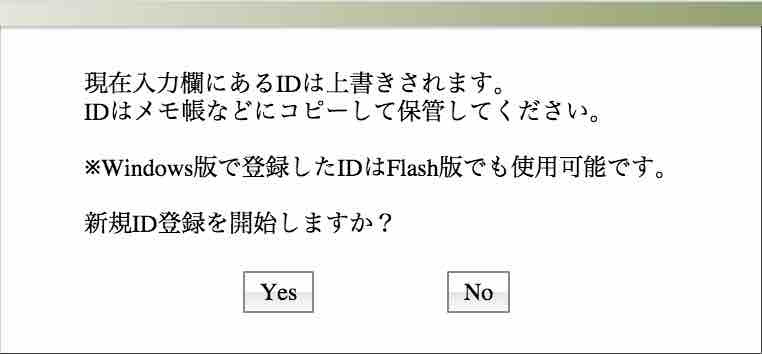
\includegraphics[width=.6\textwidth,clip]{figs/tenhou5.jpg}
\end{center}

A pop-up message will show up, warning you that whatever ID that is currently shown in the ID field (if any) will be overwritten with a new ID and that you may want to copy and paste the current ID (if any) into some text file or similar. Do so if you do see an old ID in the ID field, just to be safe. If the ID field is blank, just click the Yes button, which will open yet another pop-up message. 

\begin{center}
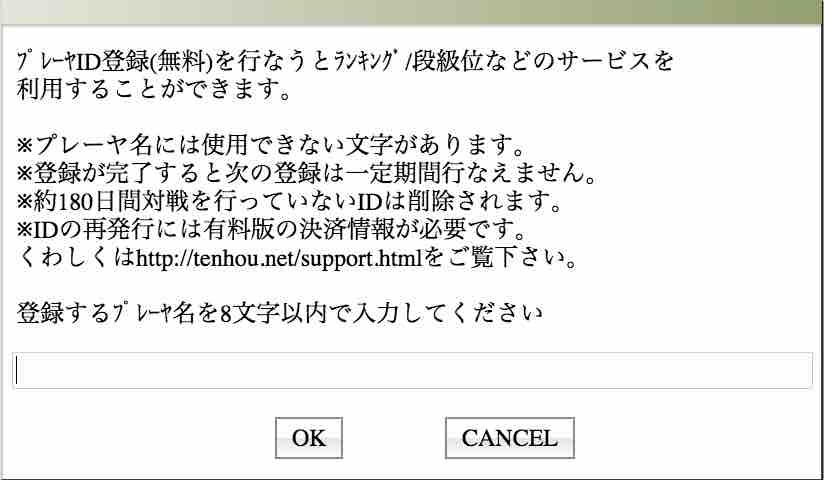
\includegraphics[width=.6\textwidth,clip]{figs/tenhou6.jpg}
\end{center}

\noindent It is telling you the following:
\bi \itemsep0.1em
\i You can create a player ID for free, and doing so is necessary if you want to earn a rank ({\jap kyuu / dan}) and rating. 
\i Some characters or character combinations are not allowed in player names.
\i Once you register, you cannot register another account for a given period (7 days).
\i If you don't play for 180 days, your ID may be deleted.
\i A player name must have 1-8 characters.
\ei

Type in a player name you'd like to have (8 characters or fewer) into the blank field at the bottom and click OK. 
You cannot change your player name later, so choose wisely. If the player name you type in is already taken by another player, it gives you an error message, as follows:

%\begin{wrapfigure}{r}{60mm}
\begin{center}
\begin{overpic}[width=.5\textwidth,clip]{figs/tenhou8.jpg}
\put(10,0){\color{MyRed} This player name is taken.}
\end{overpic}
\end{center}
%\vspace{-10pt}
%\end{wrapfigure}

Click OK, and type in another name. If successful, you'll see a new message asking you to confirm that you want to register an account with the player name provided. 

\begin{center}
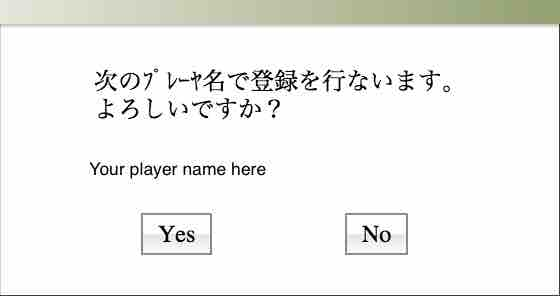
\includegraphics[width=.55\textwidth,clip]{figs/tenhou9.jpg}
\end{center}

%\bigskip

\noindent Click Yes and you'll see another message as follows:
\begin{center}
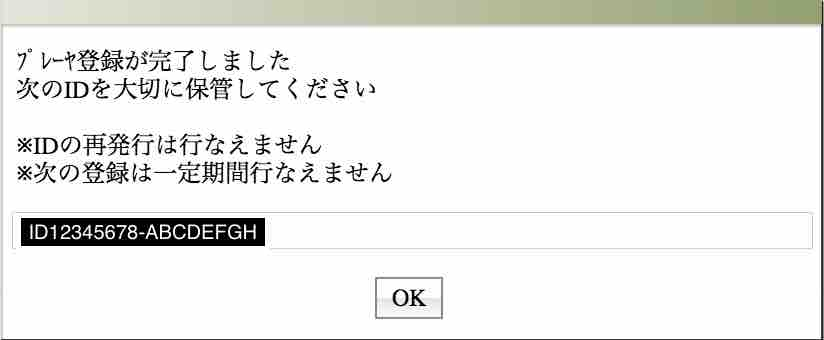
\includegraphics[width=.8\textwidth,clip]{figs/tenhou10.jpg}
\end{center}

The 19-digit alpha-numeric code that starts with ``ID'' (shown in white on a black background) is your unique player ID (it is ID12345678-ABCDEFGH in the picture above). I suggest you save your ID in a text file or something so that you don't lose it. They cannot re-issue your player ID (unless you have a paid membership and hold a rank of 七段 or higher). 

\bigskip

Clicking OK will take you back to the log-in entrance page, but this time you should see your player ID in the ID field.

%\bigskip
\begin{center}
\begin{overpic}[width=.8\textwidth,clip]{figs/tenhou11.jpg}
\linethickness{2pt}
\put(80,-10){\color{MyRed}\vector(1,1){37}}
\put(10,-20){\color{MyRed}\small Your player ID}
\put(160,-10){\color{MyRed}\vector(0,1){33}}
\put(100,-22){\color{MyRed}\small Choose 男 (male voice) or 女 (female voice)}
\put(210,70){\color{MyRed}\vector(-1,-2){20}}
\put(200,110){\color{MyRed}\small Can choose}
\put(190,93){\color{MyRed}\small プレミアム or}
\put(200,75){\color{MyRed}\small エコノミー.}
\end{overpic}
\vspace{10pt}
\end{center}

\bigskip
You can make several choices before entering the main page. First, you can choose male or female voice (for {\jap pon} / {\jap chii} / riichi, etc.) by clicking on the button right next to the ID field. You can choose a different gender each time you log in to the main lobby. Second, you can choose プレミアム (premium) or エコノミー (economy) version. The premium version has better graphics, so I suggest you choose the premium version. 

\bigskip
If you are happy with your choices, you can enter the main page by clicking on the OK button on the right. 

\newpage

\section{The main page}

Here is what the {\jap Tenhou} main page looks like when you first log on in. 
The right half of the main page shows your statistics (currently all the fields are blank because you haven't played any games), and the left half shows the games you can play and some other features. 

\bigskip

\begin{center}
\begin{overpic}[width=.8\textwidth,clip]{figs/tenhou_lobby.jpg}
\linethickness{2pt}
\put(25,-15){\color{MyRed}\small Menu}
\put(70,-15){\color{MyRed}\small Cancel (to cancel a reservation)}
\put(43,-7){\color{MyRed}\vector(0,1){18}}
\put(102,-7){\color{MyRed}\vector(0,1){18}}
\put(-45,140){\color{MyRed}\small Main tabs}
\put(-40,120){\color{MyRed}\small Sub tabs}
\end{overpic}
\end{center}

\bigskip

In the second line of the left hand side, you see three numbers. In the example above, they are 1857, 915, and 118 (the numbers will be different on your screen). These numbers show that 1857 players are currently online, 915 players are waiting, and 118 players are about to finish their games. 

\bigskip
Below these three numbers, there are six main tabs, which read 段位戦, 雀荘$\beta$, 技能$\beta$, 観戦, 牌譜, and ヘルプ. The 段位戦 tab is the main lobby where we play games (段位戦 reads {\jap dan-i-sen} in Japanese; it means ranking matches). Under the 段位戦 tab, there are four sub-tabs, which read 一般, 上級, 特上, and 鳳凰, corresponding to four different rooms. At first you can only play at tables in the 一般 room. 
Let's first go to the 段位戦 tab, and choose the 一般 sub-tab. 

\subsection*{Making reservations}
In each of the four rooms (i.e., 一般, 上級, 特上, and 鳳凰), there are 12 different variants of riichi mahjong games you can choose from. 

\bigskip

Games in the left column (under 東風戦 {\jap tonpusen}) are East-only games,\footnote{In a special circumstance where no player gets 30000 or more points by the end of East-4, the game continues into the South round.} and games in the right column (under 東南戦 {\jap tonnansen}) are more standard East-South games that have both East and South rounds.\footnote{Just like East-only games, when there is no player who has 30000 or more points by the end of South-4, the game continues into the West round. 
}

\begin{center}
\begin{overpic}[width=.6\textwidth,clip]{figs/ippan.jpg}
\linethickness{2pt}
\put(-68,110){\color{MyRed}\small Closed {\jap tanyao}}
\put(-64,91){\color{MyRed}\small Open {\jap tanyao}}
\put(-67,69){\color{MyRed}\small With red fives}
\put(-23,50){\color{MyRed}\small Fast}
\put(-60,31){\color{MyRed}\small Three-player}
\put(-40,12){\color{MyRed}\small Fast (3p)}
\put(62,-10){\color{MyRed}\small East-only}
\put(130,-10){\color{MyRed}\small East--South}
%\put(220,120){\color{MyRed}\vector(-1,0){20}}
\put(183,112){\color{MyRed}\small 1 player waiting}
\put(183,97){\color{MyRed}\small 44 players playing}
\end{overpic}
\end{center}


\bigskip
Games in the first row (喰断ナシ {\jap kuitan nashi}) are unusual games where open {\jap tanyao} (All Simples) is not allowed; you have to have a concealed hand to claim {\jap tanyao}.\footnote{{\jap kuitan} means ``open {\jap tanyao}'' and {\jap kuitan nashi} means ``without {\jap kuitan}'' in Japanese.} There is no red five in these games, either. 
Open {\jap tanyao} is allowed in all the other games. Games in the second row are more standard games with open {\jap tanyao}, but they do not have red fives. 
Games in the third row have three red fives. This is arguably the most standard type of riichi mahjong game played in Japan as of now. 
Games in the fourth row have the same rule as those in the third, but the time limit on each action is more strict. 
Games in the fifth and sixth rows are three-player games, where open {\jap tanyao} and red fives are both allowed. 

\bigskip
The set of numbers delimited by a colon in each cell represent the numbers of players currently waiting and playing the game, respectively. For example, the first row in the left column shows 3:24, which means that 3 players are waiting in queue after signing up for a game, and 24 players are currently playing East-only, closed {\jap tanyao} games. As it happens, East-South games with red fives are usually the most popular on {\jap Tenhou}, followed by East-only, fast games. 

\bigskip
To sign up for a game, click on the \fbox{予約} (reservation) button in the corresponding cell. You can make as many reservations as you want; you will be given a seat at a table that first becomes available. If you make multiple reservations, other reservations will be automatically canceled when you start playing at another table. To cancel all the reservations at once, click on the \fbox{キャンセル} (Cancel) button at the bottom right of the left-hand side of the main page. The cancel button becomes active (clickable) only after you make a reservation. 

\newpage
\section{Playing a game}

\begin{wrapfigure}{r}{50mm}
\vspace{-20pt}
\begin{center}
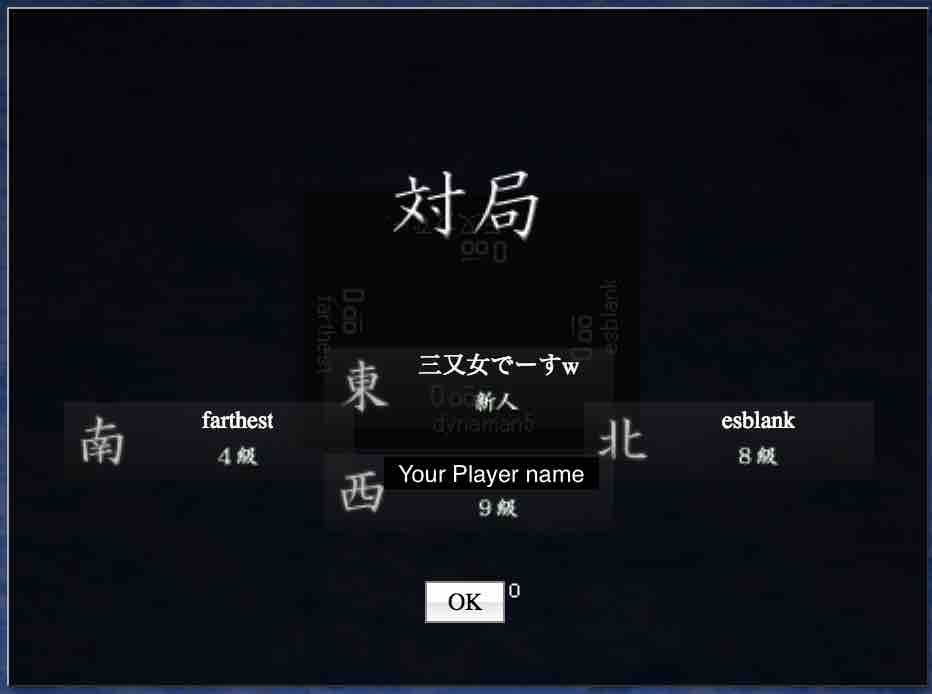
\includegraphics[width=.45\textwidth,clip]{figs/taikyoku}
\end{center}
\vspace{-20pt}
\end{wrapfigure}

Once a slot becomes available for you, you will be taken to a game table along with three other players. A black pop-up screen (see right) will appear. The game will start in 10 seconds (if all the four players click on the OK button, the game will start immediately). Each player is randomly assigned to East, West, South, or North. In the example below, my initial seat wind is North (北). 

\bigskip
The {\jap Tenhou} interface is quite intuitive so you won't need much instruction. 
Once a hand begins, tiles are dealt automatically. You also automatically draw a tile when your turn comes. 
In each turn, click on the tile you want to discard. 

%\begin{wrapfigure}{r}{60mm}
\begin{center}
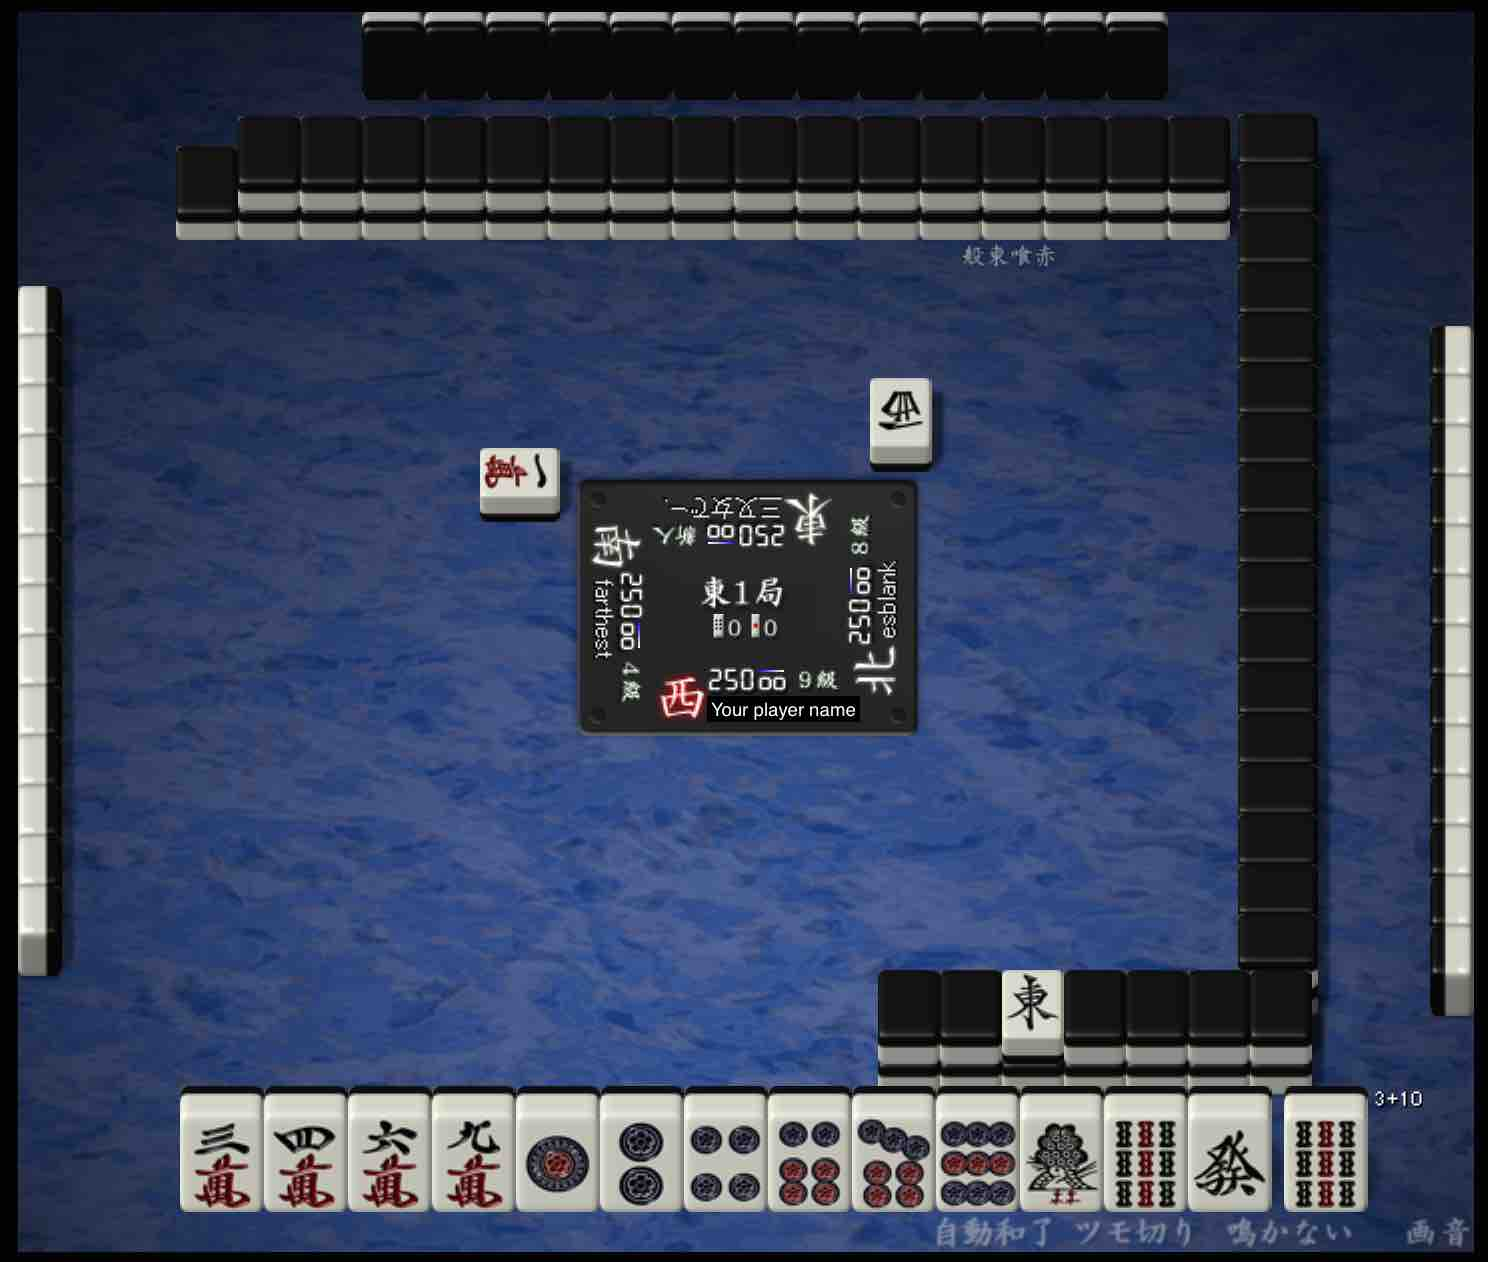
\includegraphics[width=.6\textwidth,clip]{figs/interface.jpg}
\end{center}
\vspace{-25pt}
%\end{wrapfigure}

\bigskip
Each action is timed. At a standard (non fast) table, you have 5 seconds to discard a tile. In addition, you are given a total allowance of 10 seconds in each hand. That is, even when you use up the 5 seconds allocated to you in a particular turn, you will be given the maximum of additional 10 seconds (minus the seconds you have already used up in previous turns in the hand). For example, when you use 5 + 4 seconds in the first turn, the remaining allowance reduces to $10 - 4$ = 6 seconds in this hand. Therefore, the next time you use up the first 5 seconds, you will be given only 6 more seconds. The allowance will increase by 1 second (up to 10 seconds) each time you make your discard choice in less than 1 second. The allowance will revert to 10 seconds when the next hand begins. At fast tables, each action must be done in 3 seconds, with a total allowance of 5 seconds.

\subsection{Calling / melding}
When a call becomes available, a box with a call name will show up to prompt your reaction. 
The call prompts are written in Japanese. The good news is that they are relatively simple and easy to guess from the context. It would be enough to memorize the following eight mahjong words in Japanese. 

\subsubsection{1. リーチ riichi \textipa{[r\'\textsci\textlengthmark t\textesh]}} 
You can call riichi when you have (1) a closed ready hand, (2) at least 1000 points left, and (3) at least one turn left to draw. When all of the three conditions are met, a translucent box that reads リーチ in white letters will pop up in your turn. 
\begin{center}
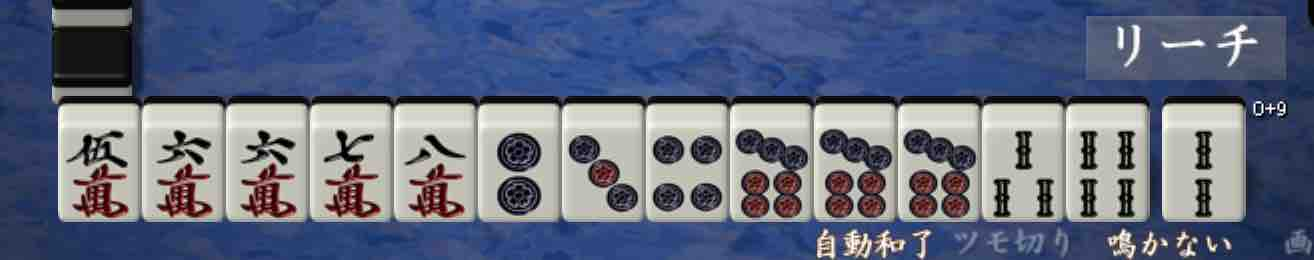
\includegraphics[width=.7\textwidth,clip]{figs/riichi.jpg}
\end{center}
If you want to riichi, you \underline{must click on the リーチ box first}, then click on the tile you want to discard. Once you click on the リーチ box, you cannot call it off. Clicking on the リーチ box also makes it impossible to discard a tile that does not make the hand ready. In the above example, tiles other than {\LARGE \wan{5}\wan{6}\wan{8}\tong{7}} will become unclickable once you click on the リーチ box. If you do not want to call riichi, just click on the tile you want to discard. 

\subsubsection{2. ロン {\jap ron} \textipa{[r\'\textopeno\ng]}}
A ロン box will pop up whenever you can legitimately declare {\jap ron} on an opponent's discard. In other words, {\jap chombo} is made impossible on {\jap Tenhou}. For example, when you are {\jap furiten}, a ロン box will not pop up because you cannot legally {\jap ron} with a {\jap furiten} hand. Whenever your hand is in a {\jap furiten} status, it is indicated with a フリテン ({\jap furiten}) sign in small translucent letters below your hand that looks like: 
\includegraphics[width=.12\textwidth,clip]{figs/furiten.jpg}.
If you don't click on the ロン box in time (i.e., in 5 or 3 seconds + allowance), it is assumed that you pass. 

\subsubsection{3. パス Pass (do nothing)}
Whenever a ロン box pops up, another box that reads パス (pass) will accompany it. 
\begin{center}
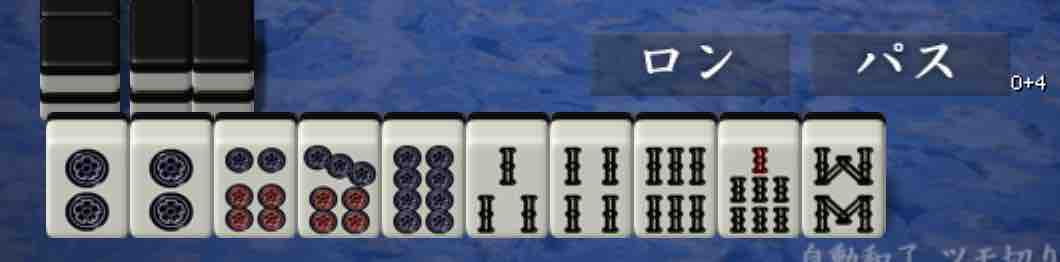
\includegraphics[width=.7\textwidth,clip]{figs/ron.jpg}
\end{center}
Click on the パス box immediately if you don't want to declare {\jap ron} on a discard. You would not want to pause for too long because that can look suspicious. A パス box will also pop up when other calling actions become available. 

\subsubsection{4. ツモ {\jap tsumo} \textipa{[ts\'umo]}}
A ツモ box will pop up when you can legitimately declare {\jap tsumo} with your draw. 

\subsubsection{5. ポン {\jap pon} \textipa{[p\'\textopeno\ng]}}
When calling {\jap pon} becomes available, a ポン box will pop up right above the tiles in your hand with which to call {\jap pon}. A パス box will also pop up. If you want to call {\jap pon}, mouseover the tiles in your hand with which to call {\jap pon}. Then the candidate tiles will stick out, as follows:
\begin{center}
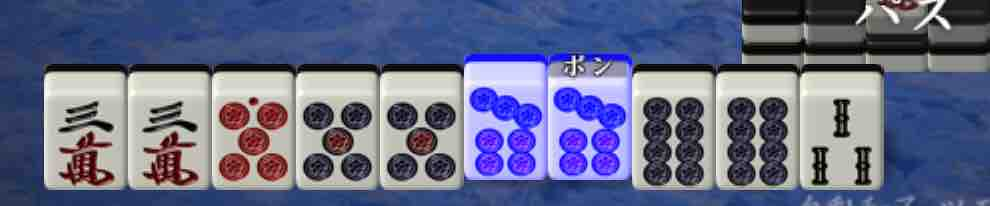
\includegraphics[width=.7\textwidth,clip]{figs/pung.jpg}
\end{center}
Click on them to call {\jap pon}. If you click on the パス box or don't do anything in time, it is assumed that you pass. 

\subsubsection{6. チー {\jap chii} \textipa{[t\textesh\'\textsci\textlengthmark]}}
{\jap Chii} calls are done in a similar way. When it becomes available, a small sign that reads チー will pop up right above the tiles in your hand with which to call {\jap chii}. 

\begin{center}
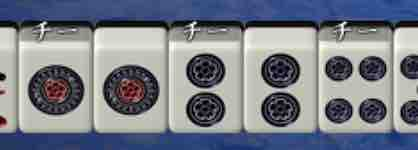
\includegraphics[width=.4\textwidth,clip]{figs/callchii_alt.jpg}
\end{center}

When you have multiple sets of tiles with which to {\jap chii}, as is the case in the above picture, mouseover the candidate tiles to choose. In the picture above, the left player discarded a {\LARGE \tong{3}} and you can {\jap chii} it with either {\LARGE \tong{1}\tong{2}} or {\LARGE \tong{2}\tong{4}}. If you want to {\jap chii} it with {\LARGE \tong{1}\tong{2}}, mouseover the {\LARGE\tong{1}} then the {\LARGE \tong{1}} and a {\LARGE \tong{2}} will stick out so you can click on them. If you want to {\jap chii} it with {\LARGE \tong{2}\tong{4}}, mouseover the {\LARGE\tong{4}} then a {\LARGE \tong{2}} and the {\LARGE \tong{4}} will stick out so you can click on them.

\subsubsection{7. カン {\jap kan} \textipa{[k\'\textturnv\ng]}}
Calling {\jap kan} on a discard is similar to calling {\jap pon}. To build a melded {\jap kan} by extending a melded {\jap pon}, you need to mouseover the melded {\jap pon} until a small sign that reads カン appears below the {\jap pon}. To call a concealed {\jap kan}, mouseover the four tiles you want to {\jap kan} then the tiles will stick out, accompanied by a small sign that reads カン below them. Click on them to call {\jap kan}. 

\subsubsection{8. 九種九牌 {\jap Kyuushu Kyuuhai}}
When you have nine different terminals and honors after the first draw in an uninterrupted first set of turns, you can declare an abortive draw. When this becomes available, a box that reads 九種九牌 will pop up. Click on it if you want to declare an abortive draw. If you wish to continue with the hand, just click on the tile you want to discard. 

\subsubsection{Multiple boxes}

Sometimes you have multiple choices as to what to do with a given discard of your opponent. 
In the following example, you have a ready hand waiting for {\LARGE \wan{2}-\wan{5}}, and the left player discarded a {\LARGE \wan{5}}. You will be given the following three choices: 

\begin{center}
\begin{overpic}[width=.6\textwidth,clip]{figs/ron_pass.jpg}
\linethickness{2pt}
\put(97,68){\color{MyRed}\large {\jap Ron}}
\put(145,68){\color{MyRed}\large Pass}
\put(-30,30){\color{MyRed}\large {\jap Chii}}
\end{overpic}
\end{center}

\bi\itemsep.1em
\i Call {\jap ron}
\i Call {\jap chii}
\i Pass (do nothing)
\ei
To call {\jap ron} on the discarded {\LARGE \wan{5}}, click on the ロン ({\jap ron}) box that pops up above your hand. If you want to do nothing, click on the パス (pass) box right next to the ロン box. Alternatively, if you want to call {\jap chii}, mouseover the two tiles you want to {\jap chii} with (in this case {\LARGE \wan{3}\wan{4}}) and click on them. 


\subsection{Buttons}

The buttons at the bottom right corner allow you to toggle on/off some calling-related features. Each feature is turned off at the beginning of a new hand. 

\bigskip

\begin{center}
\begin{overpic}[width=.8\textwidth,clip]{figs/choices.jpg}
\put(-10,-13){\color{MyRed}\small Auto call win}
\put(50,25){\color{MyRed}\small Auto discard draw}
\put(170,-13){\color{MyRed}\small No call}
\put(230,-13){\color{MyRed}\small Picture (画)}
\put(240,25){\color{MyRed}\small Sound (音)}
\end{overpic}
\end{center}

\bigskip

\subsubsection{自動和了 (Auto call win)} 
If you turn this on, you will automatically win a hand when possible without clicking on ロン or ツモ boxes. In other words, the option of passing is unavailable when this is turned on. Keep in mind that this can be problematic at times when you intend not to win your hand from a particular opponent or on a particular tile. When this is turned on, the word 自動和了 is shown in white; when it is turned off, it is translucent. In the picture above, it is turned on. 

\subsubsection{ツモ切り (Auto discard draw)} 
If you turn this on, you will automatically discard whatever tile you draw. Turn this on when you have to go to toilet or somewhere but don't want to quit the game entirely. When you riichi, this feature is automatically (and implicitly) turned on. In the picture above, it is turned off. 

\subsubsection{鳴かない (No call)}
If you turn this on, you will not be prompted to call {\jap chii}, {\jap pon}, or {\jap kan}. This feature is useful for hiding information about your hand's tile composition from your opponents. If you pause every time someone discards a certain tile you can call, your opponents might be able to guess what pairs of tiles you have and don't have. Drawing a deduction from such time lags constitutes an important skill in {\jap Tenhou}. However, in order not to disadvantage players waiting to call {\jap chii} / {\jap pon} too much, time lags will also occur randomly (i.e., even when no one can call {\jap pon} / {\jap chii} on the discarded tile). 

\subsubsection{画 (Picture) and 音 (Sound effect)}
You can change the appearance of the tiles and/or mat or resize the window with the Picture button. You can turn on/off the sound effect (for riichi, {\jap chii}, {\jap pon}, etc.) with the Sound button.

\vfill

\subsection{Scoring}
When a player wins a hand, the score will be calculated automatically. A scoring board will pop up that shows the hand, {\jap dora} (and {\jap ura dora} if riichi was declared), {\jap yaku} names and the associated number of {\jap han}, minipoints, and the total hand value. 

\begin{center}
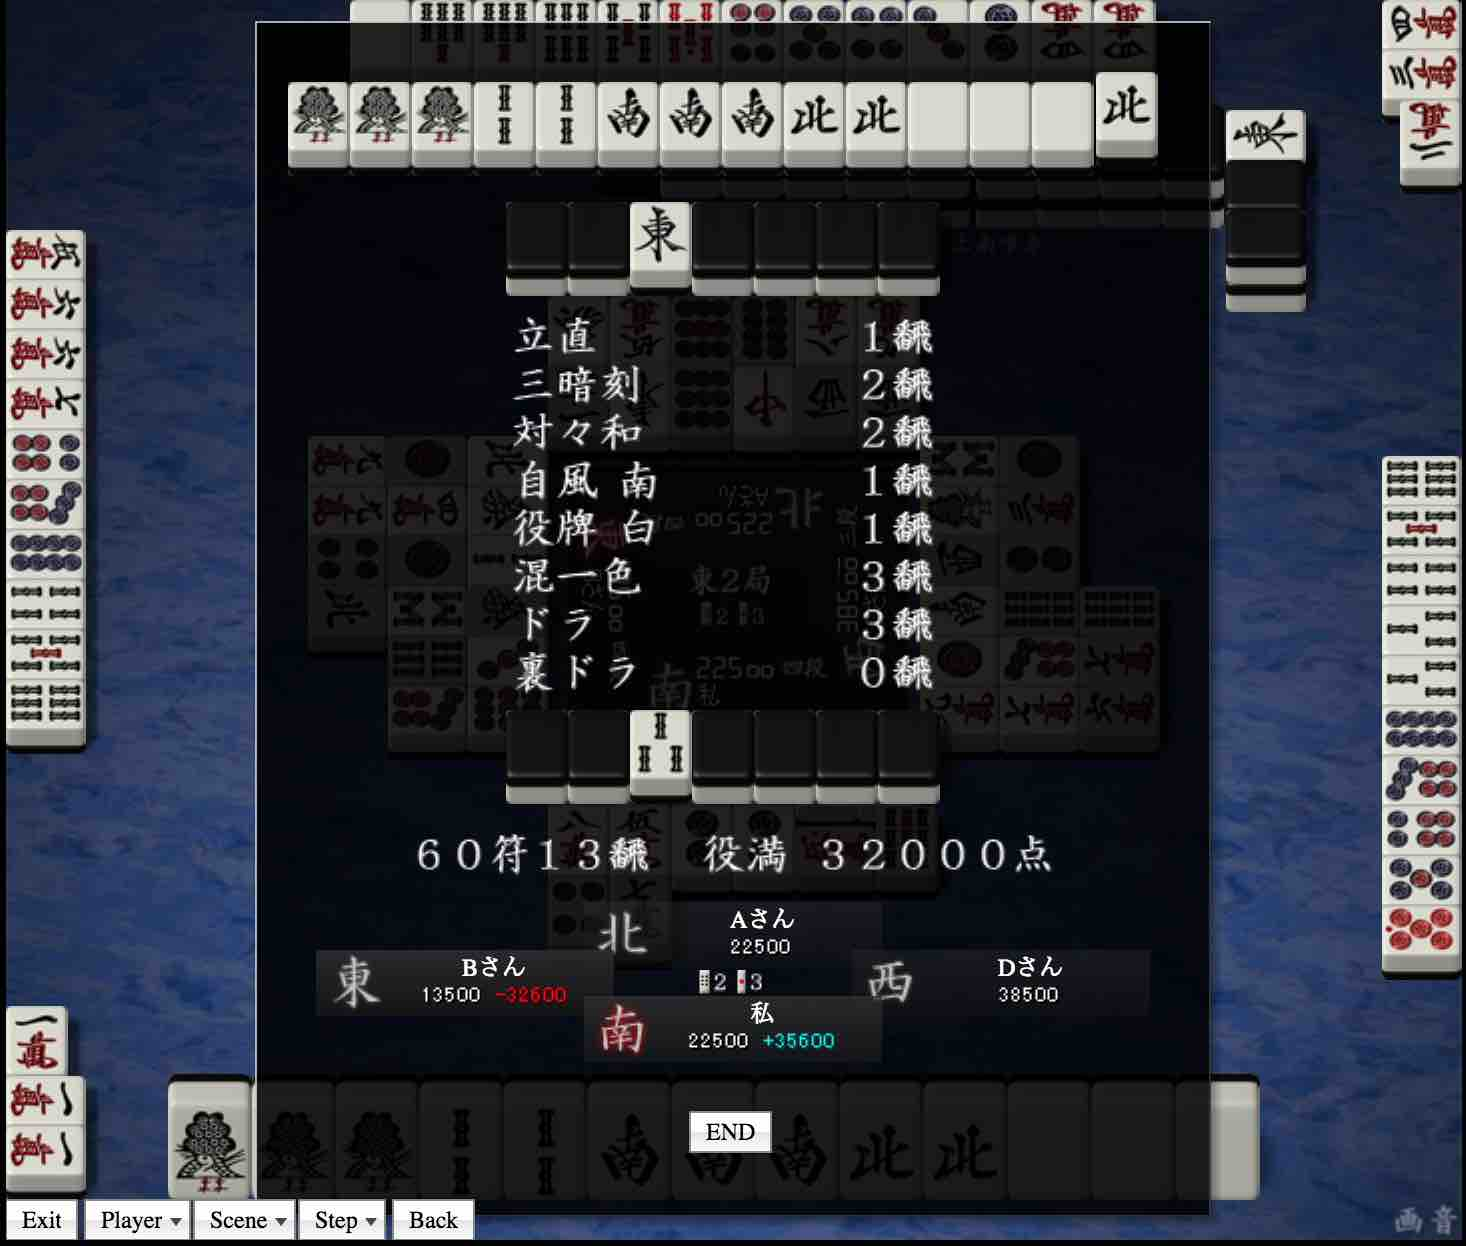
\includegraphics[width=.6\textwidth,clip]{figs/yakuman.jpg}
\end{center}
In the example above, the left player dealt into my hand that is worth 60 符 ({\jap fu}; minipoints) 13 飜 ({\jap han}) = 32000 点 (points). {\jap Yaku} names will be shown in Japanese along with {\jap han} counts. 
Table \ref{tbl:yakulist} at the end of this chapter lists all the {\jap yaku} names {\jap Tenhou} recognizes. 

\vfill

\subsection{Indicators}\label{sec:indicator}
The black rectangular board in the middle of the screen provides information about the proceeding of the game. 

\begin{center}
\begin{overpic}[width=.4\textwidth,clip]{figs/proceeding1}
\linethickness{2pt}
\put(150,82){\color{White} \vector(-2,-1){70}}
\put(-15,82){\color{White} \vector(2,-1){70}}
\put(150,80){\color{MyRed}\bf Number of}
\put(150,65){\color{MyRed}\bf riichi bets}
\put(-60,73){\color{MyRed}\bf Counter}
%\begin{overpic}[width=.4\textwidth,clip,grid]{figs/proceeding2.jpg}
\end{overpic}
\end{center}
We can see that this is South-4, there is 0 counter and 0 riichi bet, and it is the North player's turn. 
The West player is leading (44000 points), followed by the East player (26800), the North player (17400), and the South player (11800). Each player's rank ({\jap kyuu / dan}) is shown right next to their points. 

%\begin{wrapfigure}{r}{60mm}
\begin{center}
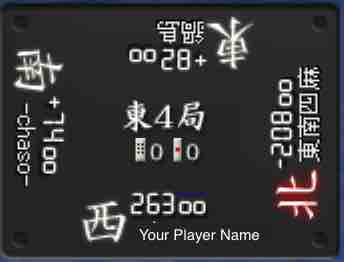
\includegraphics[width=.4\textwidth,clip]{figs/proceeding2}
\end{center}
%\vspace{-10pt}
%\end{wrapfigure}

\bigskip
If you mouseover the middle board, you will see the current point differences between you and each of your opponents. 
In the present example, the West player has $44000 - 26800 = + 17200$ more points than I do. If you are leading against another player, the point difference will be negative. For example, the South player has $11800$ so the point difference is $11800 - 26800 = -15000$. 

\bigskip
It is important to pay a close attention to these point differences, especially in the South round or when one of your opponents is at the risk of bankruptcy. In the current example, if the East player wins a 12000 hand from the South player, South will go bankrupt and the game is terminated. Notice that East is currently ranked second, having 17200 points fewer than West. In this case, winning a 12000 from South is not ideal for East because East will still be ranked second and the game is over.\footnote{As we will see later, avoiding the fourth place is more important in {\jap Tenhou} rules than it is in other rules. However, this does not mean that it is your only priority; you would still want to improve your placement in a game when doing so is a realistic possibility.}

\bigskip

You can also see the type of game you are currently playing on the board. Just below the wall opposite to you is an indicator that looks like this: 
\includegraphics[width=.2\textwidth,clip]{figs/gametype.jpg}. 
\bi
\i The first letter indicates the room: 般 for 一般 ({\jap ippan}), 上 for 上級 ({\jap joukyuu}), 特 for 特上 ({\jap tokujou}), 鳳 for 鳳凰 ({\jap houou}). See Chapter \ref{ch:Tenhou2} for explanations of these.
\i The second letter indicates if it is an East-only game (東) or an East--South (南) game.
\i The third letter indicates if open {\jap tanyao} is allowed: 喰 (with open {\jap tanyao}) or 無 (without open {\jap tanyao})
\i A fourth letter (赤) is added if there are red fives.
\i A fifth letter (速) is added if it is a fast game. 
\ei

\vfill

\subsection{Ending of a game}
A game can end in several different ways. 
\bi
\i One or more player goes bankrupt (below 0 points). 
\i South-4 (East-4 in East-only games) ends and at least one player has 30000 or more points.
\i West-4 (South-4 in East-only games) ends.
\i At any point in the West round (South round in East-only games), at least one player has 30000 or more points. 
\ei

\noindent
When a game ends, final scores are calculated as follows. 
\bi
\i In cases of a tie, the player sitting closer to the first dealer wins. 
\i {\jap Oka} (winning premium) is 20000. That is, although every player is allocated 25000 points at the beginning of a game, they have to return 30000 at the end of the game, meaning that 30000 will be subtracted from the final raw scores. \index{oka@{\jap oka}}
The residual points of 20000 $= (30000 - 25000)  \times 4$ are awarded to the winner of the game.
\i {\jap Uma} (placement bonus) is 10-20. That is, 1st player gets $+ 20000$, 2nd player gets $+ 10000$, 3rd player gets $-10000$, and 4th player gets $-20000$. \index{uma@{\jap uma}}
\i Each score is then scaled by dividing it by 1000 and rounding it off. 
\ei 

It appears that European players are not very familiar with the {\jap oka} system (possibly because there is no {\jap oka} in EMA rules), so let me explain this with an example. Suppose that players A, B, C, and D hold the following raw points at the end of a game; 39000, 25100, 22900, and 13000, as shown in Table \ref{tbl:Tenhouscore} below.\index{european@EMA}

\begin{table}[h!]\centering
\caption{Final score calculation on {\jap Tenhou}}\label{tbl:Tenhouscore}
\begin{tabular}{l r r r r}
\toprule
Player & Raw score & Before {\jap uma} & After {\jap uma} & After {\jap oka}\\
\midrule
A & $39000$ & $9000$ & $29000$ & $49000$\\
B & $25100$ & $-4900$ & $5100$ & $5100$ \\
C & $22900$ & $-7100$ & $-17100$ & $-17100$\\
D & $13000$ & $-17000$ & $-37000$ & $-37000$\\
\bottomrule
\end{tabular}
\end{table}

\bigskip
The first numerical column shows the raw scores. Then, 30000 is subtracted from each of the raw scores (second column). Then, we add {\jap uma} to each score based on placements (third column). Finally, we add {\jap oka} to the winner's score to obtain the final scores (fourth column).  

%\newpage

\begin{wrapfigure}{r}{55mm}
%\vspace{-25pt}
\begin{center}
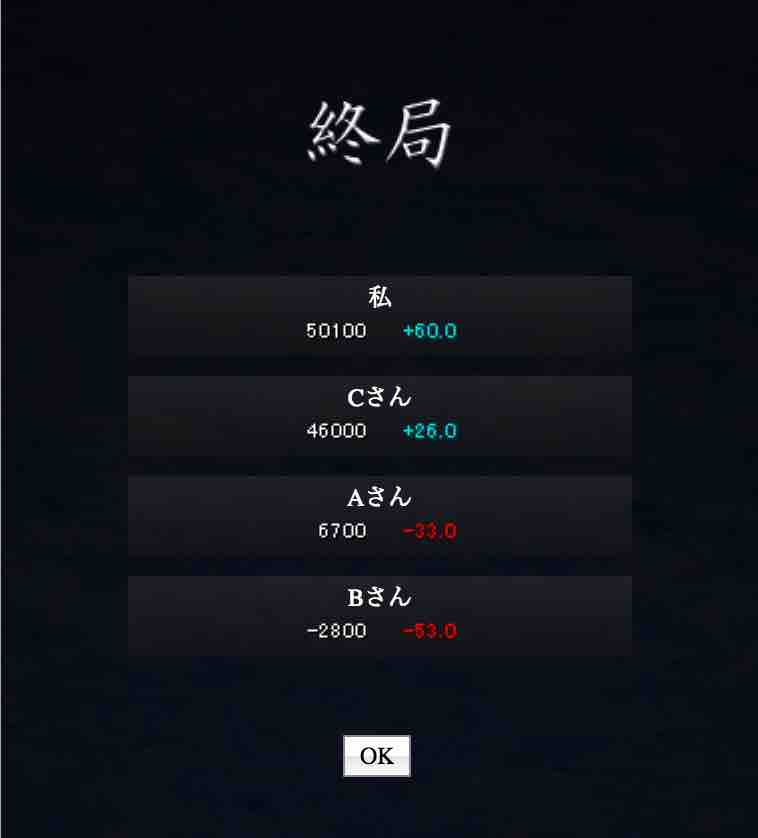
\includegraphics[width=.4\textwidth,clip]{figs/finalscore.jpg}
\end{center}
\vspace{-25pt}
\end{wrapfigure}

\bigskip

The final scores after adding {\jap uma} and {\jap oka} and scaling will be displayed along with the placements and raw scores. In the example to the right of this text, I (私 means ``me'') came in 1st, earning 50100 points (60.0 with {\jap uma} and {\jap oka}), 2nd player (C さん, which reads Mr. C) earns 46000 points (+ 26.0 with {\jap uma}), 3rd player earns 6700 points ($-33.0$ with {\jap uma}), and 4th player went bankrupt ($-2800$ points, $-53.0$ with {\jap uma}). 

\newpage

\begin{boxnote} \small
{\bf\normalsize Notes on placement}

\bigskip
It is important to keep in mind that your rank and rating on {\jap Tenhou} depend solely on the placement in a game and not on how many points you earn in a game, before or after adding {\jap uma} and {\jap oka}. In other words, there is \emph{absolutely} no difference between getting 1st place with 30000 points and getting 1st place with, say, 80000 points in terms of their contributions to your rank and rating.\footnote{You might wonder why they still calculate the final scores with {\jap uma} and {\jap oka} in {\jap Tenhou} if they are irrelevant; I honestly have no idea.}

\bigskip
This feature adds an interesting strategic element to the game. That is, it makes it clearer that the goal of mahjong is \emph{not} to win a hand \emph{per se} but to have a better placement at the end of a game. Winning a hand is just one of several means to securing a good placement. On occasion, you may find it beneficial to assist one of your opponents instead of trying to win a hand yourself. Intentionally dealing into an opponent's hand can sometimes be a good tactic when it serves the purpose of securing your own placement. 

\bigskip
In my impression, many European players are lacking the appreciation of this aspect of mahjong. I hope you will learn to appreciate it through playing lots of games on {\jap Tenhou}.
\vspace{5pt}
\end{boxnote}

\newpage
\section{Troubleshooting}

At times, you may get disconnected from the {\jap Tenhou} server (possibly because of poor internet connection on your end or problems on the server).\footnote{You will notice that players sometimes get disconnected on purpose to quit playing, especially when they are losing badly.}
When a player gets disconnected from the server during a game, the game still continues. The ``auto discard draw'' will be turned on for the disconnected player, so they will be simply discarding anything they draw until they return. The player name will turn into dark red once a player is disconnected. 

\begin{wrapfigure}{r}{60mm}
\vspace{-10pt}
\begin{center}
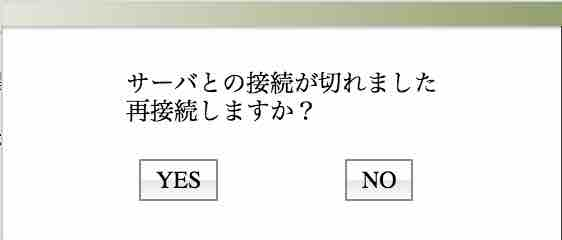
\includegraphics[width=.45\textwidth,clip]{figs/warning2.jpg}
\end{center}
\vspace{-10pt}
\end{wrapfigure}

\bigskip
When you get disconnected, you may get a warning message shown above, asking you if you would like to get connected again. Click Yes if you want to. However, a warning message does not always show up when you get disconnected. When a screen freezes during a game for more than 15 seconds, you should suspect that you are disconnected. You may want to hit the refresh button on your browser to get connected to the server again. 

\bigskip
You can create more than one accounts on {\jap Tenhou}, but you will have to wait for 7 days unless your IP address changes. If you attempt to create a second account from the same IP address within 7 days, you will get an error message shown below, telling you that you cannot create a new account from your IP address in 7 days. 

\begin{center}
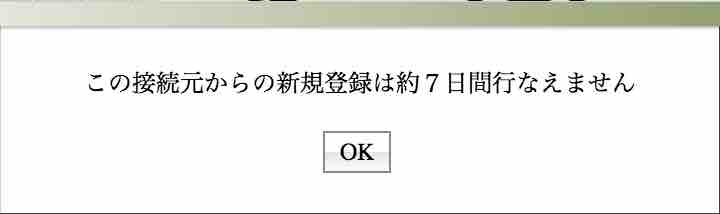
\includegraphics[width=.5\textwidth,clip]{figs/warning1.jpg}
\end{center}

\section{Rules}
Here is a summary of the rules on {\jap Tenhou}. 

\bi
\i Three red fives (one in each suit) in games with red fives.
\i No {\jap kuikae} (swap-calling). That is, you cannot discard an identical tile after {\jap pon} or {\jap chii}. You cannot discard the tile from other end of the run, either. 
\i ``Sudden death'' rule when no player has 30000 or more points after South-4 (East-4 in East-only games).
\i A game is terminated when a player goes bankrupt.
\i Automatic {\jap agariyame} rule (i.e., the game is automatically terminated if the dealer is leading after the end of South-4, even if he won a hand in South-4).
\i One-{\jap han} minimum all the time (i.e., no two-{\jap han} minimum even after five counters).
\i Abortive draw in the following situations
	\bi
	\i 九種九牌 (nine terminals / honors)
	\i 四家立直 (four riichi's)
	\i 三家和了 (three players call {\jap ron} on a discard)
	\i 四風子連打 (four players discard the same wind)
	\i 四槓散了 (four {\jap kan} by different players)
	\ei
\i 流し満貫 ({\jap nagashi mangan}) is allowed. You can declare it even when you have called {\jap pon} / {\jap chii}. You cannot declare it if one or more of your discards has been called by others.
\i Up to two players can win on a discard. riichi bets and counter bonus go to the player sitting closer to the player who discarded the winning tile. The dealership remains if the dealer is one of the winners.
\i The following are recognized as {\jap yakuman}: 
天和 ({\jap Tenhou}; Blessing of Heaven) / 地和 ({\jap chihou}; Blessing of Earth) / 大三元 ({\jap daisangen}; Big Three Dragons) / 四暗刻 ({\jap su anko}; Four Concealed Pungs) / 四暗刻単騎 ({\jap su anko tanki}; Single-Wait Four Concealed Pungs) / 字一色 ({\jap tsuiisou}; All Honors) / 緑一色 ({\jap ryuiisou}; All Green) / 清老頭 ({\jap chinroutou}; All Terminals) / 国士無双 ({\jap kokushi muso}; Thirteen Orphans) / 国士無双13面 (Thirteen-wait Thirteen Orphans) / 大四喜 ({\jap daisushi}; Big Four Winds) / 小四喜 ({\jap shosushi}; Little Four Winds) / 四槓子 ({\jap su kantsu}; Four Kongs) / 九蓮宝燈 ({\jap churenpoutou}; Nine Gates) / 純正九蓮宝燈 ({\jap junsei churenpoutou}; Nine-wait Nine Gates).
\i {\jap Yakuman} can be combined. For example, 大三元 (Big Three Dragons) can be combined with 字一色 (All Honors), 四暗刻 (Four Concealed Pungs), and either of 四槓子 (Four Kongs), 天和 (Blessing of Heaven) or 地和 (Blessing of Earth), producing a quadruple {\jap yakuman} (128000 points). 
\i There is no double {\jap yakuman} unless different {\jap yakuman} are combined. For example, 国士無双 (Thirteen Orphans) and 国士無双13面 (Thirteen-wait Thirteen Orphans) are both single {\jap yakuman}. 
\i You cannot call {\jap pon} / {\jap chii} / {\jap kan} on the last discard in a hand. 
\i {\jap Sekinin barai}: a player who feeds the third Dragon {\jap pon} / {\jap kan} to an opponent with two melded Dragon {\jap pon} / {\jap kan} must pay the full value of the hand in case Big Three Dragons is made on a self-draw. In case another player deals into it, the two share the payment equally. The same rule applies to Big Four Winds, but not to {\jap rinshan kaihou} (After a Kong).  
\ei


\bigskip

{\begin{table}[h!]\centering
\footnotesize \captionsetup{font=footnotesize}
\caption{List of {\jap yaku} names} \label{tbl:yakulist}
\begin{tabularx}{11.5cm}{l l X l}
\toprule
{\jap Yaku} & Pronunciation & EMA name & {\jap Han} (open)\\
\midrule
門前清自摸和 & {\jap (menzen-) tsumo} & Fully Concealed Hand & 1 (NA)\\
立直 & riichi & Riichi & 1 (NA)\\
一発 & {\jap ippatsu} & Ippatsu & 1 (NA)\\
槍槓 & {\jap chankan} & Robbing the Kong & 1\\
嶺上開花 & {\jap rinshan kaiho} & After a Kong & 1\\
海底摸月 & {\jap haitei (-moyue)} & Under the Sea & 1\\
河底撈魚 & {\jap houtei (-raoyui)} & Under the River & 1\\
自風  & {\jap jikaze} & Seat Wind & 1\\
場風  & {\jap bakaze} & Prevailing Wind & 1\\
役牌 & {\jap yakuhai} / {\jap fanpai} & Dragon Pung & 1\\
断幺九 & {\jap tanyao} & All Simples & 1\\
一盃口 & {\jap iipeiko} & Pure Double Chow & 1 (NA)\\
平和 & {\jap pinfu} & Pinfu & 1 (NA)\\
混全帯幺九& {\jap chanta} & Outside Hand & 2 (1)\\
一気通貫& {\jap ittsu} & Pure Straight & 2 (1)\\
三色同順& {\jap sanshoku (-doujun)} & Mixed Triple Chow & 2 (1)\\
三色同刻& {\jap sanshoku doukou} & Mixed Triple Pungs & 2\\
両立直 & double riichi & Double Riichi & 2 (NA)\\
三槓子 & {\jap san kantsu} & Three Kongs & 2\\
対々和 & {\jap toitoi} & All Pungs & 2\\
三暗刻 & {\jap san anko} & Three Concealed Pungs & 2\\
小三元 & {\jap shousangen} & Little Three Dragons & 2\\
混老頭 & {\jap honroutou} & {\scriptsize All Terminals and Honors} & 2\\
七対子 & {\jap chiitoitsu} & Seven Pairs & 2 (NA)\\
純全帯幺九 & {\jap junchan} & Terminals in All Sets & 3 (2)\\
混一色 & {\jap honitsu} & Half Flush & 3 (2)\\
二盃口 & {\jap ryanpeiko} & Twice Pure Double Chow & 3 (NA)\\
清一色 & {\jap chinitsu} & Full Flush & 6 (5)\\
流し満貫 & {\jap nagashi mangan} & -- & {\jap mangan}\\
ドラ & {\jap dora} & Dora & \\
赤ドラ & {\jap aka dora} & Red five & \\
裏ドラ & {\jap ura dora} & Ura dora & \\
\bottomrule
\end{tabularx}
\end{table}}

%~~~~~~~~~~~~~~~~~~~~~~~~~~~~~~~~~~~~~~~~~~~~~~~~~
% Riichi Book 1, Chapter 2: tenhou guide 2
%~~~~~~~~~~~~~~~~~~~~~~~~~~~~~~~~~~~~~~~~~~~~~~~~~
\chapter{Advanced features of {\jap tenhou}} \label{ch:tenhou2}
\thispagestyle{fancy}

\section{Rank and rating}

\begin{floatingtable}[r]{
\footnotesize \captionsetup{font=footnotesize}
\centering 
\begin{tabular}{l r r r}
\toprule
Rank & N & Rank & N\\
\midrule
天鳳位	&9\\
十段	&15&	1級	&7780\\
九段	&130&	2級	&5849\\
八段	&592&	3級	&6481\\
七段	&1830&	4級	&6383\\
六段	&3140&	5級	&6971\\
五段	&5968&	6級	&9964\\
四段	&9957&	7級	&16606\\
三段	&14436&	8級	&14509\\
二段	&18174&	9級	&28283\\
初段	&15046&	~~~新人&132411\\
\bottomrule
\end{tabular}}
\caption{Player distribution} \label{tbl:rank}
\end{floatingtable}

{\jap Tenhou} offers two different player rating systems --- rank ({\jap kyu / dan}) and R (rate). 
The {\jap kyu / dan} ranking system is similar to the one commonly used in Japanese arts, games, and martial arts. 
The {\jap kyu} (級) ranks are shown in arabic numbers, going from 9級 to 1級 in descending order. After passing 1級, you enter the {\jap dan} (段) ranks, shown in {\jap kanji} numbers, going from 初段 (一段; first {\jap dan}) to 十段 (tenth {\jap dan}) in ascending order. Everyone starts with {\jap 新人} (newbie; no rank), and if you pass the 十段 rank, you are awarded the highest rank called 天鳳位 ({\jap tenhoui}). Since the inception of {\jap tenhou} in 2006, there have been only nine players who have achieved 天鳳位 at the time of writing this book. 
Table \ref{tbl:rank} shows the distribution of active players holding each rank as of 20 December, 2015. 

\bigskip

\subsection{{\jap kyu / dan} rank}

To advance your {\jap kyu / dan} rank, you need to earn points (called ``pt'' or ``段位 pt'' on {\jap tenhou}). For example, to proceed from the 新人 (newbie) status to the 9 級 ({\jap kyu}) rank, you need to earn 30 points. Required amount of points for promotion gets greater and greater as you move further up. For example, to proceed from 六段 (sixth {\jap dan}) to 七段 (seventh {\jap dan}), you need to earn as many as 1200 points. 

\bigskip
To find out how many more points you need to earn to advance to the next rank from the current rank, see the top right part of the main page. 

\bigskip

\begin{center}
\begin{overpic}[width=.5\textwidth,clip]{figs/rank2.jpg}
\linethickness{2pt}
\put(-15,35){\color{MyRed} \vector(3,-1){70}}
\put(-90,36){\color{MyRed}\small\bf Your current}
\put(-90,16){\color{MyRed}\small\bf rank (7級)}
\put(175,45){\color{MyRed} \vector(-2,-1){70}}
\put(175,50){\color{MyRed}\small\bf pt you have / }
\put(175,30){\color{MyRed}\small\bf pt you need }
\put(120,-13){\color{MyRed} \vector(0,1){15}}
\put(100, -20){\color{MyRed}\small\bf Your R}
\end{overpic}
\vspace{10pt}
\end{center}
\noindent In this example, the player currently holds the rank of 7級. The part that reads ``30 / 60 pt'' means that she has earned 30 points since she became 7級 and that she needs 60 points in total to be promoted to 6級. 

\bigskip
When you rise or fall in rank, your points will be reset to a default value. For {\jap kyu} rank players, the default value is 0 points. For {\jap dan} rank players, the default value is different depending on ranks. For example, the default points for 六段 players are 1200 points. When they get 1200 more points and reach 2400 points, they get promoted to 七段. When they lose all the initial 1200 points and reach 0 points, they get demoted to 五段. 

\bigskip

The amount of points you earn or lose in each game depends on your placement (but \emph{not} scores with {\jap uma} and {\jap oka}), the type of game (East-only or East--South), the room in which the game is played (一般, 上級, 特上, or 鳳凰), and your current rank.\footnote{Points you earn or lose in East-only games are two-thirds of those in East--South games.} 
You gain positive points only if you come in first or second place. 
If you come in first place, you will gain the following points regardless of your rank.

\bi \itemsep-.5em
	\i 45 points in the 一般 ({\jap ippan}) room
	\i 60 points in the 上級 ({\jap joukyu}) room
	\i 75 points in the 特上 ({\jap tokujou}) room
	\i 90 points in the 鳳凰 ({\jap houou}) room
\ei
If you come in second place, you will gain the following points regardless of your rank.
	\bi \itemsep-.5em
	\i 0 points in the 一般 room
	\i 15 points in the 上級 room
	\i 30 points in the 特上 room
	\i 45 points in the 鳳凰 room
\ei
You don't gain or lose points if you come in third place. 
The points you lose when coming in fourth place depend on your rank but not on the room. When your rank is 3級 or below, you lose 0 point. However, each time your rank rises above 3級, the points you lose get bigger by 15 points. 
That is, 2級 players lose 15 points if they come in fourth place; 1級 players lose $15 \times 2 = 30$ points; 初段 players lose $15 \times 3 = 45$ points, ... , and 十段 players lose as many as 180 points if they come in fourth place.

\bigskip
Notice how severe the punishment is for coming in fourth, and it gets severer and severer as your rank goes up. This is one of the distinctive features of {\jap tenhou}. 
Avoiding the fourth place tends to be players' top priority in {\jap tenhou} games. This is in contrast to standard mahjong games, where the reward for coming in first usually outweighs the cost of coming in fourth, thanks to the {\jap oka} system.\footnote{Recall that, although {\jap tenhou} does adopt the {\jap oka} system, it is the placement, not the scores, that determines the points you earn or lose. In this sense, EMA games are actually more similar to {\jap tenhou} games than to standard games.\index{european@EMA} Since there is no {\jap oka} in EMA games, the reward for coming in first is much smaller than that in standard games.} \index{oka@{\jap oka}}

\bigskip
\begin{wrapfigure}{t}{50mm}
\vspace{-30pt}
\begin{center}
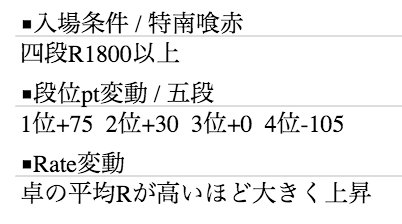
\includegraphics[width=.45\textwidth,clip]{figs/pt}
\end{center}
\vspace{-40pt}
\end{wrapfigure}
To easily find out how many points you earn / lose for each place in a given type of game for your rank, mouseover the \fbox{予約} button in each cell on the left-hand side of the main page. Then, you will see something like the picture above on the right-hand side of the main page. Under the second bullet point, we see that, for this player's rank (五段), the point reward is: +75 for first place, +30 for second place, 0 points for third place, and $-105$ for fourth place. 

\bigskip
\begin{wrapfigure}{r}{60mm}
\vspace{-30pt}
\begin{center}
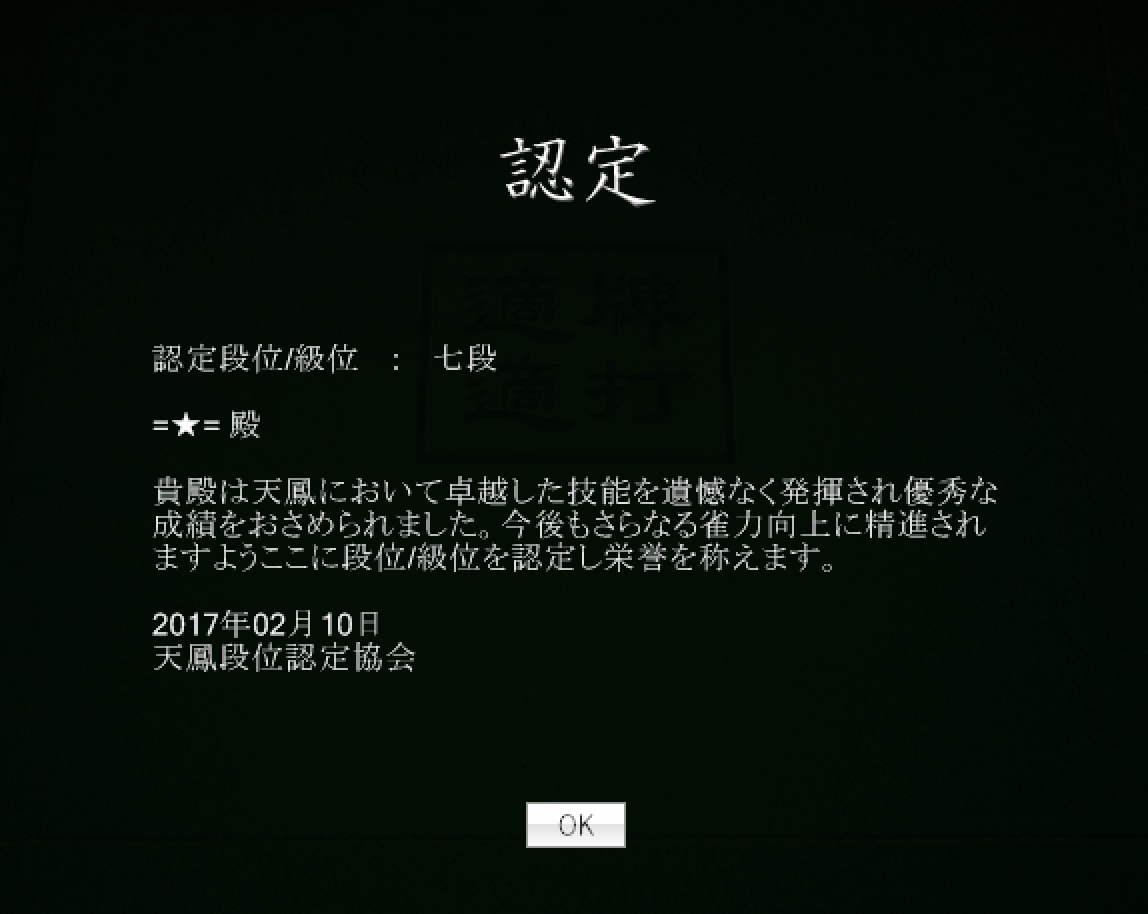
\includegraphics[width=.45\textwidth,clip]{figs/7dan}
\end{center}
\vspace{-25pt}
\end{wrapfigure}
When you have earned enough points for promotion in a game, a new rank is awarded after the game. A certificate message like the picture to the right of this text will pop up after the game. 

\bigskip
Since you never get negative points in games until you reach 2級 and there is no demotion until you reach 初段 (first {\jap dan}), it should be relatively easy to reach 初段. In fact, even without studying the contents of this book, you can perhaps reach as high as 四段 (fourth {\jap dan}) if you play two hundred games or so. However, moving further up will probably require that you study basic strategies and tile efficiency theories. 

\subsection{Rate (R)}

In addition to the {\jap kyu / dan} rank, {\jap tenhou} gives each player another rating called R. The initial value of R is 1500, and higher-rank players tend to have a higher R. For example, the average R among the 天鳳位 players is 2248.%\footnote{In case you are curious, the highest R I have reached as of December 2015 is 2106.}

\bigskip
While {\jap kyu / dan} rank remains relatively stable, R can change after each game. R is calculated based on your placement in a game, but it also depends on the average R of the players you play with. 
A change in R after a game, $\Delta R$, is calculated with the following formula:
\begin{align*}
\Delta R &= (P + \bar{R}) \times G
\end{align*}
where 
\bi \itemsep-.5em
\i $P$ is based on your placement in the game: + 30 for first, +10 for second, $-$10 for third, and $-$30 for fourth;
\i $\bar{R}$ is an adjustment that reflects how strong your opponents are, calculated as (Average R in the game $-$ your R) $/$ 40; and
\i $G$ is an adjustment based on $n$, the number of games you have played before. If $n \leq 400$, G is equal to $1-0.002 \times n$. If $n > 400$, G is set equal to 0.2.
\ei

\bigskip
R initially fluctuates a lot, as the scaling factor $G$ is very close to 1 until you play many games. R may go up or down by 30 or so for each of the first 100 games or so. As you play more games, however, the fluctuation gets smaller and smaller as $G$ approaches to $0.2$. 

\bigskip
Notice what the adjustment $\bar{R}$ does. This factor is positive when you play against players who are ``stronger'' than you (i.e., have a higher R than you) while it is negative when you play against players who are ``weaker'' than you. Therefore, when you win against stronger players, your reward will be bigger than when winning against weaker players. Likewise, when you lose against weaker players, your punishment will be severer than when losing against stronger players. 
Because of these features, one might say that your R better reflects your skill levels than your {\jap kyu / dan} rank. 

\section{Four rooms}
As we have seen, there are four different rooms where ranking matches are played. Qualifications to play in each room are based on your rank and R. 

\subsection*{1. 一般 ({\jap ippan}; lower-level room)}
This is the only room where you can play initially. Players with an R higher than 1800 and a rank higher than 四段 are not allowed to play here, however. Games in this room can sometimes be a bit random, even chaotic at times. Some of the players in this room probably do not understand the rules very well. You very rarely come across strong players here. 

\subsection*{2. 上級 ({\jap joukyu}; upper-level room)}
You can play here if (1) your rank is 1級 or higher or (2) you buy a two-month membership (\textyen~1080 = \euro~8 = \textsterling~6).\footnote{If you want to pay for the membership, click on the link that appears when you click the 上級 sub-tab. Keep in mind that you need to buy 60 days' worth of membership. Choose ``60日分を購入(1080円)'' in the payment page.} Players with an R higher than 2000 and a rank higher than 七段 are not allowed to play in this room, however. 

\bigskip
Games in the {\jap joukyu} room are more reasonable than those in the lower-level room, but you still see many players who do not defend at all, do meaningless {\jap dama} / unreasonable {\jap riichi}, and make serious mistakes in maximizing tile efficiency. In my impression, games at EMA tournaments most resemble games in the {\jap ippan} and {\jap joukyu} rooms.\index{european@EMA} 

\subsection*{3. 特上 ({\jap tokujou}; advanced room)}
Requirements to play in this room are pretty demanding. You have to have a 四段 or higher rank and a 1800 or higher R. The latter requirement is particularly difficult to satisfy for intermediate players. As I wrote above, achieving the rank of 四段 is not that difficult, but satisfying the R $>$ 1800 condition requires that you take mahjong rather seriously. Since weak players are shut out from the {\jap tokujou} room, games in {\jap tokujou} are qualitatively different from those in the {\jap joukyu} and {\jap ippan} rooms. Games in this room feel similar to those you'd experience at regular フリー ({\jap furii}) mahjong parlors in Japan. 

\subsection*{4. 鳳凰 ({\jap houou}; phoenix room)}
This is the highest-level room in {\jap tenhou}. In order to play in this room, you have to have all of the following: (1) a 七段 or higher rank, (2) a 2000 or higher R, and (3) a paid membership (\textyen~540 yen = \euro~4 = \textsterling~3 per month). Satisfying the first two conditions can be really, really challenging. 

\bigskip
This is arguably one of the highest-level mahjong locales in the whole world. It is not uncommon for you to come across a {\jap houou}-level player at a regular mahjong parlor in Japan. However, you usually play against at most one {\jap houou}-level player at a table, and the two other players at the table are either {\jap tokujou}- or {\jap joukyu}-level players. What is remarkable about games in the {\jap houou} room is that you will be surrounded by three other {\jap houou}-level players. 
It would be safe to say that no other public mahjong locale in the world --- whether it is online or offline --- could offer a comparable experience.\footnote{Perhaps the highest-level leagues in professional mahjong associations in Japan have higher-quality players, but you have to become a professional player to play at such leagues. Even after becoming a professional, you will need at least a few years to reach the highest league.}

\section{Reading the statistics}
After you play 30 games or so, you may want to start paying attention to the statistics shown on the right-hand side of the main page.\footnote{There is really no point in reading too much into the statistics when you have played only a few games; the sample size is too small to be meaningful.} 
The upper half of the player statistics shows your statistics for the entire period, whereas the bottom half shows your statistics in the present month for a given type of game in a given room. 

\bigskip
\subsection{Overall statistics}
The picture below show my old player statistics (upper half) back from when I had a 二段 rank. 
Let me explain how to read these statistics. 

\begin{center}
\vspace{-10pt}
\begin{overpic}[width=.6\textwidth,clip]{figs/stats1_anon.jpg}
\linethickness{2pt}
\put(-52,98){\color{MyRed}\small Entire period}
\put(133,98){\color{MyRed}\small (4-player games)}
\put(-60,62){\color{MyRed}\small first place}
\put(-60,49){\color{MyRed}\small second place}
\put(-60,36){\color{MyRed}\small third place}
\put(-60,23){\color{MyRed}\small fourth place}
\put(-60,10){\color{MyRed}\small bankruptcy}
\put(210,62){\color{MyRed}\small win rate}
\put(210,49){\color{MyRed}\small deal-in rate}
\put(210,36){\color{MyRed}\small call rate}
\put(210,23){\color{MyRed}\small {\jap riichi} rate}
\end{overpic}
\vspace{-10pt}
\end{center}

Below a player name is the expiration date of my paid membership (17 November, 2015). When I started playing {\jap tenhou} on 17 September, 2015, I bought a 60-day membership so I can play in the {\jap joukyu} room. If you have just created a {\jap tenhou} account, the expiration date may be shown as today's or tomorrow's date, meaning that your ID may be deleted if you don't play any games. When you play two or three games, it will turn into ``----/--/--'', meaning that your ID will not be deleted for another 180 days. If you don't play any game for 180 days, your account may be deleted. 

\bigskip

The box below the expiration date that reads 全期間 / 段位戦 4人打ち indicates that the statistics below are for the entire period (not just this month) and for 4-player games (not 3-player games). Below that, we see that I had a 二段 rank, 565 points (the initial 400 points plus 165 points earned after I became 二段) out of the 800 points I need for promotion, and an R of 1987. 

\bigskip

Three columns below these display my statistics. The first column shows my placement rates. I had come in first place 50\% of the games, second place 32.5\%, third place 7.5\%, fourth place 10 \%, and gone bankrupt 7.5\% of the games. Ideally, you'd want your first place rate to be greater than your second place rate, your second place rate greater than your third place rate, etc. 

\bigskip

The middle column provides the following information. First, 対戦数 shows the number of games you have played. At this point, I had played 40 games. Second, 平均得点 shows the average score (with {\jap oka} and {\jap uma}) from all the games I have played. As I said before, this does not influence your R nor rank. Third, 平均順位 shows the average placement. If you have obtained each of the four places equally, the average placement would be 2.5 $\left( \frac{1  n + 2  n + 3  n + 4 n}{4n} = 2.5 \right)$. Therefore, any values below 2.5 indicate that you are, on average, winning more than losing. 
The two rows that follow (shown in light gray) are relevant only if you play games in private rooms. Since I have only played ranking matches, they are left blank. 

\bigskip

The third column shows my statistics based on hand-level performance. First, 和了率 ({\jap houra} rate; {\jap agari} rate; win rate) is the number of hands you have won divided by the total number of hands you have played in all games.\footnote{The denominator includes hands where no one won.} 

\bigskip
Second, 放銃率 ({\jap houju} rate; deal-in rate) is the number of times you have fed the winning tile to an opponent's hand divided by the total number of hands you have played. You would want this rate to be lower, but keep in mind that (1) sometimes you would be better off dealing into an opponent's hand to secure your placement, and (2) sometimes you need to discard dangerous tiles (which would increase your deal-in rate, on average) in order to increase the chance of winning your hand (which would increase your win rate, on average). The rule-of-thumb is that the difference between your win rate and deal-in rate (win rate - deal-in rate) should be at least 10 percentage points. That is, if you have a high deal-in rate, you need your win rate to be higher. Likewise, if you have a low deal-in rate, it is OK to have a lower win rate as well. 

\bigskip
Third, 副露率 ({\jap fuuro} rate; call rate) is the number of hands where you have called {\jap chii} / {\jap pon} / {\jap kan} divided by the total number of hands you have played. Finally, 立直率 ({\jap riichi} rate) is the number of {\jap riichi} calls you made divided by the number of hands you have played. 

\bigskip

The ranking page on {\jap tenhou}\footnote{\url{http://goo.gl/suyQ5}} has a table that summarizes the average values of these statistics among players with different ranks (under the heading that reads 段位戦4人打ち平均戦績). You may want to compare your statistics with the average values among players who share your rank or those who have higher ranks than you do. Figure \ref{fig:avg} summarizes the average values of hand-level performance statistics for players in different ranks. 

\begin{figure}[t!] \captionsetup{font=small}
\begin{center}
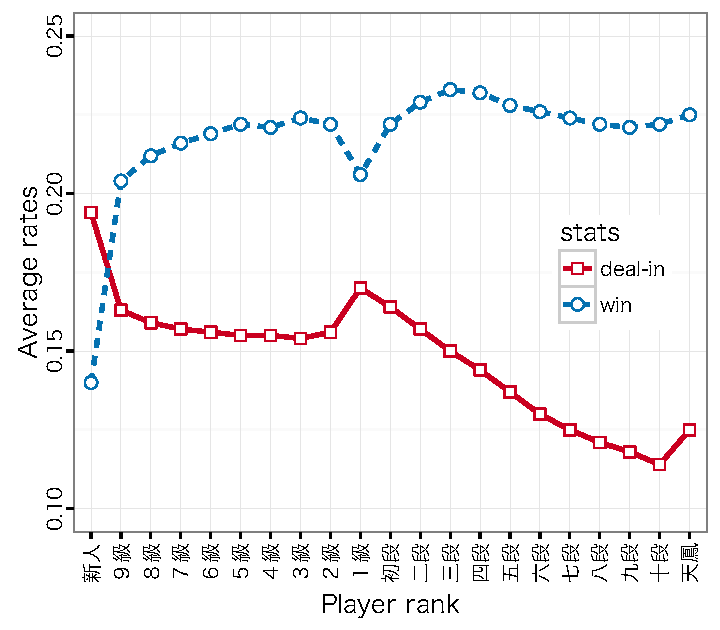
\includegraphics[width=.50\textwidth,clip]{figs/stats_wd.pdf}\hspace{-7pt}
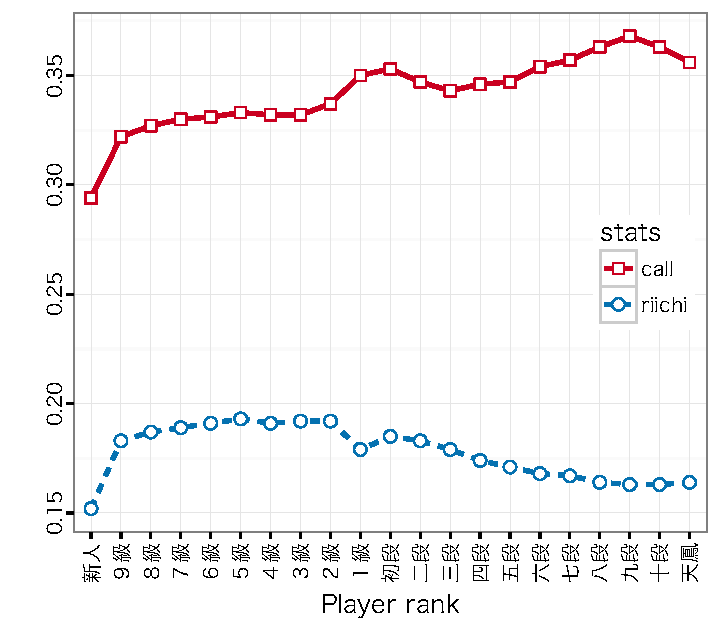
\includegraphics[width=.50\textwidth,clip]{figs/stats_cr.pdf}
\vspace{-10pt}
\caption{Average hand-performance statistics}\label{fig:avg}
\end{center}\vspace{-10pt}
{\footnotesize \textit{Note:} These graphs show the hand-performance statistics reported in a table on the ranking page (\url{http://goo.gl/suyQ5}) as of 20 December, 2015.}
\end{figure}

\bigskip
We can see some interesting patterns here. The left-hand side panel compares average win rates (和了率) and deal-in rates (放銃率) for different ranks. Notice that the average win rate is relatively constant across different ranks; once you pass the 新人 rank, it stays around 20-22 \%. 

\bigskip
On the other hand, the average deal-in rate is steadily decreasing after players move from the {\jap kyu} ranks into the {\jap dan} ranks. It is around 15\% for almost all {\jap kyu} rank players (except for 新人 and 1級), but it keeps going lower and lower as players rise in the {\jap dan} rank. The fact that high-{\jap dan} players have lower deal-in rates on average is remarkable, considering that they are facing stronger opponents than low-{\jap dan} players do. This pattern signifies the importance of defensive skills.

\bigskip

Another interesting thing to notice on the left-hand side panel is that the average scores deteriorate once you move from 2級 to 1級 (i.e., average win rate gets lower, and average deal-in rate gets higher). 

\bigskip
I can think of two reasons for why this happens. First, 1級 is where most players start playing in the {\jap joukyu} (upper-level) room, where average player skills are much higher than those in the {\jap ippan} (lower-level) room. If a player who belongs to the lower-level room plays in the upper-level room, their performance will necessarily go down, making it look that 1級 players are worse than 2級 players even if they are not. Second, if you keep losing as a 初段 (first {\jap dan}) player, you get demoted to 1級 but you will never be demoted to 2級. This means that 1級 players might actually be worse than 2級 players, on average. 

\bigskip

The right-hand side panel shows the average call rates (副露率) and {\jap riichi} rates (立直率) for different ranks. The former is increasing as rank goes up, while the latter is decreasing, but the changes are rather gradual for both rates. 

\subsection{Monthly statistics}
The bottom-right part of the main page shows monthly statistics from games you have played in a given room. The box is a pull-down menu that lets you choose the room (一般, 上級, 特上, 鳳凰) and game type (East-only, East--South, with or without open {\jap tanyao}, red fives, etc.). In the example above, the box reads 月間 / 上南 喰アリ赤, which means the following: 月間 means monthly, 上 is short for 上級 ({\jap joukyu})\footnote{Likewise, 般 is short for 一般 ({\jap ippan}), 特 is for 特上 ({\jap tokujou}), 鳳 is for 鳳凰 ({\jap houou}).}, 喰アリ赤 means with open {\jap tanyao} and red fives.

\begin{center}
\vspace{-10pt}
\begin{overpic}[width=.6\textwidth,clip]{figs/stats2.jpg}
\linethickness{2pt}
\put(-15,105){\color{MyRed}\small Cumulative}
\put(170,105){\color{MyRed}\small Average}
\put(-23,92){\color{MyRed}\small Scores}
\put(-47,80){\color{MyRed}\small Placement}
\put(-45,26){\color{MyRed}\small first place}
\put(-45,11){\color{MyRed}\small fourth place}
\end{overpic}
\vspace{-10pt}
\end{center}


Below the box, you see the raw placement scores. In this example, 17+11+3+4 = 35戦 means that I have played 35 games this month, and I came in first place in 17 games, second place in 11 games, third place in 3 games, and fourth place in 4 games. R shown here (1987) should be the same as the R you see in the top part. 3382位 means that R=1987 puts me in 3382th place among all the active players on {\jap tenhou}. 

\bigskip
Two columns follow, where the left column shows the monthly cumulative values and the right column shows the monthly average values. 
In the first row that reads 得点 shows the monthly cumulative or average scores from 上南 喰アリ赤 games (after adding {\jap oka} and {\jap uma}). In this example, my cumulative score is 727 from the 35 games I played, which puts me in 106th place among players who have played 30 or more 上南 喰アリ赤 games this month. Similarly, my average score is 20.7 (= 727/35), which puts me in 5th place. Your placement for average scores will not be shown unless you have played 30 or more games of a given type in a given room in a given month. 

\bigskip
In the second row that reads 順位 shows cumulative or average placement from games. The cumulative placement is based on placement values (+30, +10, $-$10, or $-$30), whereas the average placement is based on raw placement (1, 2, 3, or 4). 
The 総合 (total) score is the sum of four placements: cumulative 得点, cumulative 順位, average 得点, and average 順位. In this example, I earn 106th, 80th, 5th, and 3th places for these scores, so my total score is 106+80+5+3 = 194 (the lower, the better), which puts me in 12th place among all the players who have played 30 or more 上南 喰アリ赤 games this month. 
At the bottom, you see トップ率 (first place rate),  ラス率 (fourth place rate), and 連対率 (first or second place rate) for 上南 喰アリ赤 games this month. 

\section{Viewing the games}
\subsection{Replaying the games (牌譜)}
{\jap tenhou} keeps the record of all the games played there, giving each game a unique URL. 
You can easily take a look at any of the last 40 games you have played on the 牌譜 ({\jap haifu}; game record) tab on the main page. Click on any of the 牌譜 link shown in the 牌譜 tab to start a replay of the game. You can choose to view the game from any of the four players' viewpoint, not to show the hands of the other three players, or to go back and forth between turns / hands, etc. When we play mahjong, we often wonder what the opponents are doing (e.g., what are their waits? are they doing {\jap honitsu}?, etc.). You can find out the answers to these questions after the game by taking a look at the game record. 

%\bigskip

%\begin{wrapfigure}{r}{60mm}
\begin{center}
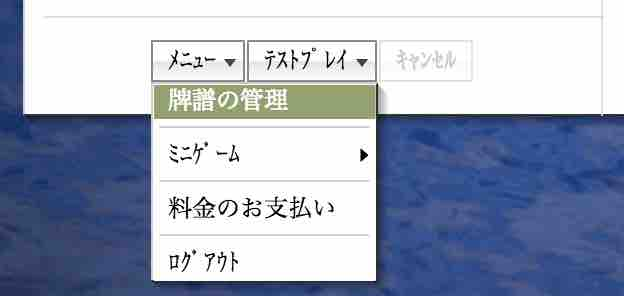
\includegraphics[width=.4\textwidth,clip]{figs/haifukanri.jpg}
\end{center}
%\vspace{-20pt}
%\end{wrapfigure}

If you would like to have someone take a look at a particular game you played to ask for their opinions, you need to find the unique URL assigned to the game you want to show. You can find out the URLs of the last 40 games by going to the 牌譜の管理 menu from the メニュー pull-down on the main page. 
Clicking on 牌譜の管理 will open a new pop-up screen.

\bigskip
You can choose to open a game replay in the current window (このウィンドウで開く), in a new pop-up window (新しいポップアップで開く), or in a new window (新しいウィンドウで開く) from the pull-down menu above. Once you are happy with your choice, click on one of the 再生 (replay) link next to the game you want replayed. 
You will be taken to a page that looks like the one you saw after clicking on the Play button on the top page of {\jap tenhou}. You can now find out the URL assigned to the game in the URL field of your browser. 

\bigskip
To start a replay, click on a link that reads >> Flash版牌譜ビューアで開く shown at the bottom of the page. Clicking on the HTML+JS版牌譜ビューアで開く link will also work, but this one is the low-quality picture version with limited options. 

\subsection{Spectating the games (観戦)}
You can watch games played in the 特上 ({\jap tokujou}; advanced) and the 鳳凰 ({\jap houou}; phoenix) rooms quasi-real time (with a five-minute delay). Click on the 観戦 ({\jap kansen}; spectating) tab from the main page and you will see the list of games you can watch. Click on one of the player name links to start spectating the game from the chosen player's viewpoint. 



%~~~~~~~~~~~~~~~~~~~~~~~~~~~~~~~~~~~~~~~~~~~~~~~~~
%			Part 2: tile efficiency
%~~~~~~~~~~~~~~~~~~~~~~~~~~~~~~~~~~~~~~~~~~~~~~~~~

\part{Basic Tile Efficiency} \label{part:tile}

%~~~~~~~~~~~~~~~~~~~~~~~~~~~~~~~~~~~~~~~~~~~~~~~~~
% Riichi Book 1, Chapter 3: Basics
%~~~~~~~~~~~~~~~~~~~~~~~~~~~~~~~~~~~~~~~~~~~~~~~~~
\chapter{Riichi mahjong basics}\label{ch:basic}
\thispagestyle{empty}

\section{Learning strategies, nya\textasciitilde}

U-um, so, nya, Mahjong is like, a game of both skill and luck, nya\textasciitilde! You
can learn all these cool strategy thingies to get better, but, um, even if
you’re super skilled, that doesn’t mean you’re always gonna win, nya! (\textit{paws
nervously}) And, um, sometimes a player who doesn’t know what they’re doin’
can totally beat the big, strong players just ‘cause of, um, luck, nya\textasciitilde!

In the short run, nya, luck kinda decides who wins and loses more than skill
does, nyaaa\textasciitilde! \footnote{
Oh, oh, and, um, an interesting question comes up here, nya! How short is
“short,” meow\textasciitilde? Like, um, how many games do you hafta play to tell the strong
players from the weaker ones, nya\textasciitilde? Studies say we’d need, um, at least 100
games (whoa, that’s a lot, meow\textasciitilde!) to get a reliable idea of our skill levels,
nyaaa\textasciitilde!
}(\textit{wobbles})
B-but, um, if you wanna be good in the long run, learning strategy stuff is
suuuper important, nya! Plus, um, it makes the game more fun when you
understand all the cool, deep stuff about it, nya\textasciitilde! (\textit{purrs excitedly})

\bigskip

Oh, oh, and, nya, because Mahjong is like, um, all probabilistic (whoa, big
word, nya!), even makin’ the best choice doesn’t always mean you’ll get the
best results, nya\textasciitilde! (\textit{tilts head}) The best choices are the ones that
give you the best chance of winnin’ on average, nya\textasciitilde! So, um, when you’re
lookin’ at your choices, you gotta think all statistically and stuff, nya\textasciitilde! (\textit{looks
a little confused but determined})

\bigskip

For example, nyaaa\textasciitilde! Look at this hand over here, nya\textasciitilde! (\textit{paws at page
excitedly})

\begin{screen}
\bp
\mahjong[25pt]{4m4m6p6p7p1s2s3s6s7s8s-666'z}
\ep
\vspace{-10pt}What would you discard? \vspace{-5pt}
\end{screen}

\bigskip
\noindent

This hand is like, ready to win if you throw away either this tile {\mahjong[15pt]{6p}} or that one {\mahjong[15pt]{7p}}, nya\textasciitilde!
But, um, which one should you discard, nyaaa\textasciitilde? Let’s compare the two choices and
see, nya\textasciitilde! (\textit{paws at the tiles excitedly})

\bi\itemsep.1pt
\i Discard {\mahjong[15pt]{6p}} $\Rightarrow$ you wait for {\mahjong[15pt]{5p} \mahjong[15pt]{8p]}} (2 kinds--8 tiles)
\i Discard {\mahjong[15pt]{7p}} $\Rightarrow$ you wait for {\mahjong[15pt]{4m} \mahjong[15pt]{6p]}} (2 kinds--4 tiles)
\ei

Nyaa\textasciitilde!\@ Oh, um, I see, meow!\@  So, like, if you discard {\mahjong[15pt]{6p}}, you get a, um, 2-way wait for {\mahjong[15pt]{5p}} and {\mahjong[15pt]{8p}}, nya!\@ And if you discard {\mahjong[15pt]{7p}}, you get a, uh, 2-way wait for {\mahjong[15pt]{4m}} and {\mahjong[15pt]{6p}}, nyaaa\textasciitilde!\@ The {\mahjong[15pt]{5p} \mahjong[15pt]{8p}} wait is, like, way better, meow!\@

\bigskip


Which discard choice is better, nya\textasciitilde? Although both of the two choices give
you a 2-way wait, nyaaa, waiting for {\mahjong[15pt]{58p}} is soooo
much better than waiting for {\mahjong[15pt]{4m6p}}
probabilistically speaking, nya\textasciitilde! With the {\mahjong[15pt]{58p}} wait, there
are four tiles of {\mahjong[15pt]{8p}} and another four tiles
of {\mahjong[15pt]{5p}} to win on, nya\textasciitilde! That’s like, um, at most
eight winning tiles, nyaaa\textasciitilde!\footnote{
    O-of course, nya,
    the number of winning tiles could be less than eight if, um, some of them have
    already been thrown away, nyaaa\textasciitilde! (paws at air nervously)

}(\textit{wiggles tail excitedly})

But, um, with the {\mahjong[15pt]{4m6p}} wait, nya,
you’ve already used up two tiles of {\mahjong[15pt]{4m}} and two tiles of {\mahjong[15pt]{6p}}
yourself, nyaaa\textasciitilde! That means you’re left with at most four winning tiles, nya\textasciitilde!
(\textit{ears droop}) It’s suuuper clear, nya, that you should choose the {\mahjong[15pt]{58p}} wait over the {\mahjong[15pt]{4m6p}} wait, 'cause
that gives you a better chance to win this hand, nya\textasciitilde! (\textit{paws at the tiles
excitedly})

\bigskip

It’s possible, nya, that after you decided on the {\mahjong[15pt]{58p}}
wait, your opponents might, um, not discard {\mahjong[15pt]{5p}} or {\mahjong[15pt]{8p}}
at all, nya\textasciitilde! Instead, they might discard a bunch of {\mahjong[15pt]{4m6p}}
tiles, nyaaa\textasciitilde! (\textit{looks frustrated but cute}) This is just the kinda
thing that happens all the time in Mahjong, nya\textasciitilde! (Or, um, in any game of
luck, nya\textasciitilde!) When this happens, nya, don’t think you made a bad choice, nya!
You didn’t, nyaaa\textasciitilde! You made the right call, but you were just, um, unlucky,
nya\textasciitilde! (\textit{sniffles}) When you get this kinda bad luck, nya, you just gotta
keep calm
and carry on, nya\textasciitilde! (\textit{puffs out chest determinedly})

\bigskip

Before talking about, um, a paws-on method to make your tile efficiency
super good in the next chapter, nya\textasciitilde! This kitty will first discuss some basic
tile efficiency principles in this one, nya\textasciitilde! While doin’ so, nya, I’ll also
introduce some important key terms you’ll see later, nyaaa\textasciitilde! Oh, oh, and I’ll
give you the original Japanese term for each one, nya! (\textit{points at the cute
font}) I do this 'cause you might see these terms used in online strategy
stuff in English, nya\textasciitilde! (\textit{wags tail proudly})

%\section{Basic building blocks}
%
%\subsection{Tiles}
%
%Mahjong tiles can be classified into two categories \textendash\textendash number tiles and honor tiles, nya\textasciitilde!\@
%\subsubsection{Number tiles}
%
%\begin{itembox}[c]{Number tiles}
%\centering
%\begin{tabular}{l c c}
%{Cracks (characters)} & {\jap Manzu} & {\mahjong[25pt]{123456789m}}\\ [\sep]
%{Dots (circles)} & {\jap Pinzu} & {\mahjong[25pt]{123456789p}}\\ [\sep]
%{Bamboos} & {\jap Souzu} & {\mahjong[25pt]{123456789s}}\\
%\end{tabular}
%
%\end{itembox}
%
%\bigskip \noindent
%Nyaa\textasciitilde! S-so, um, we can, like, classify number tiles even more, nyaaa!\@ *excited tail wiggle* There are, um, {\bf simples} ({\jap tanyao hai}, nya!), which are, like, the tiles from 2 to 8, meow! A-and then there are {\bf terminals} ({\jap yaochu hai}, nyaaa!), which are, um, 1 and 9, meow! *pauses, thinking* O-oh, they’re, um, different ‘cause they work for different {\jap yaku}, nya! A-and they also, um, change the minipoints ({\jap fu}) you get, meow!
%\index{terminal tiles}
%	\index{fu@{\jap fu} (minipoint)} \index{minipoint ({\jap fu})}

%\bigskip
%It has become quite common to include some red five tiles. For example, most games on {\jap Tenhou} have one red five tile in each suit, {\mahjong[15pt]{0m0p0s}}. These tiles are included in place of regular fives; we have three regular fives and one red five in each suit. Red fives are treated as {\jap dora} regardless of the {\jap dora} indicator. When a 4 in a given suit is the {\jap dora} indicator, the red five in that suit will be a double {\jap dora} tile.
%
%\vfill
%\subsubsection{Honor tiles}
%\index{honor tiles ({\jap jihai})} \index{jihai@{\jap jihai} (honor tiles)}
%
%\begin{itembox}[c]{Honor tiles}
%\centering \footnotesize
%\begin{tabular}{l c c c c}
%Dragon tiles & {\Huge\bai} & {\Huge\fa} & {\Huge\zhong}\\
%& White ({\jap haku}) & Green ({\jap hatsu}) & Red ({\jap chun})\\ \\
%Wind tiles &{\Huge\dong} &{\Huge\nan}& {\Huge\xi}& {\Huge\bei}\\
%& East ({\jap ton}) &South ({\jap nan}) & West ({\jap sha}) &North ({\jap pei})\\
%\end{tabular}
%\end{itembox}
%
%	\index{value tiles ({\jap fanpai; yakuhai})}
%	\index{fanpai@{\jap fanpai} ({\jap yakuhai}; value tiles)}
%	\index{yakuhai@{\jap yakuhai} ({\jap fanpai}; value tiles)}
%	\index{valueless wind@valueless wind ({\jap otakaze})}
%	\index{otakaze@{\jap otakaze} (valueless wind)}
%\noindent Some honor tiles are {\bf value tiles} ({\jap fanpai / yakuhai}); we get one {\jap han} if we collect three identical value tiles. All dragon tiles are value tiles regardless of the round and seating. On the other hand, the value status of wind tiles depends on the round and the seating. East tiles are value tiles for everyone during the East round, and South tiles are value tiles for everyone during the South round. In addition, each player gets their own seating wind as a value tile. For example, West tiles are value tiles only for the West player, but they are valueless wind tiles ({\jap otakaze}) for other players.
%
%\vfill
%\subsection{Group ({\jap mentsu})}
%\index{run ({\jap shuntsu}; chow)}
%\index{chow ({\jap shuntsu}; run)}
%\index{shuntsu@{\jap shuntsu} (run; chow)}
%\index{set ({\jap kotsu}; pung)}
%\index{pung ({\jap kotsu}; set)}
%\index{kotsu@{\jap kotsu} (set; pung)}
%\index{mentsu@{\jap mentsu} (group)}
%\index{group ({\jap mentsu})}
%\index{kan@{\jap kan} (kong)} \index{kantsu@{\jap kantsu} (quad)}
%\index{quad@quad ({\jap kantsu})}
%
%One of the major goals in playing mahjong is to win a hand.\footnote{Another important goal is not to deal into an opponent's hand. See Chapter \ref{ch:defense} for discussions of defense strategies. However, the most important goal of all is to win a game. Winning a hand and playing defense are merely two means to this end. See Chapter \ref{ch:grand} for more discussions of this.}
%To win a standard hand, we need to complete four groups ({\jap mentsu}) and one head ({\jap atama}; final pair).\footnote{There are three exceptions to this; {\jap chiitoitsu} (Seven Pairs), {\jap kokushi musou} (Thirteen Orphans), and {\jap nagashi mangan} (All Terminals and Honors Discard) do not require four groups and one head.}
%Groups can be classified into two kinds --- {\bf run} and {\bf set}.\footnote{EMA rules refer to run as ``chow'' and set as ``pung.'' I realize that my use of different terminology here might be confusing at first, but I hope you will get used to it soon.}
%\bi
%\i Run ({\jap shuntsu}; chow / sequence) is a set of three consecutive number tiles: e.g., {\LARGE \wan{7}\wan{8}\wan{9}}, {\LARGE \suo{3}\suo{4}\suo{5}}.
%\i Set ({\jap kotsu}; pung / triplet) is a set of three identical tiles: e.g., {\LARGE \wan{2}\wan{2}\wan{2}}, {\LARGE \fa\fa\fa}.\footnote{Technically speaking, there is a third type of groups, namely quad ({\jap kantsu}; kong), a set of four identical tiles. We treat quads as a variant of sets. See Section \ref{sec:kong} for discussions on this.}
%\ei
%
%
%\subsection{Ready and $n$-away}
%	\index{ready ({\jap tenpai})} \index{tenpai@{\jap tenpai} (ready)}
%	\index{1-away (1-{\jap shanten})}
%	\index{2-away (2-{\jap shanten})}
%	\index{3-away (3-{\jap shanten})}
%	\index{ukeire@{\jap ukeire} (tile acceptance)}
%	\index{tile acceptance ({\jap ukeire})}
%We say a hand is {\bf ready} ({\jap tenpai}) when the hand can be complete with one more tile. For example, the following hand is ready.
%\bigskip
%\begin{itembox}[r]{Ready hand}
%\bp
%\tong{3}\tong{4}\tong{5}\tong{8}\tong{8}\suo{2}\suo{3}\suo{6}\suo{7}\suo{8}\zhong\zhong\zhong
%\ep
%\end{itembox}
%This hand becomes complete with either {\LARGE\suo{1}} or {\LARGE\suo{4}}. We say that this hand waits for {\LARGE\suo{1} \suo{4}}.
%
%\bigskip
%
%We say a hand is {\bf 1-away from ready} (1-{\jap shanten}) when the hand can become ready with one more tile. For example, the following hand is 1-away from ready.
%\bigskip
%\begin{itembox}[r]{1-away hand}
%\bp
%\tong{3}\tong{5}\tong{5}\tong{8}\tong{8}\suo{2}\suo{3}\suo{6}\suo{7}\suo{8}\zhong\zhong\zhong
%\ep
%\end{itembox}
%This hand becomes ready if you draw any of {\LARGE\tong{4}\tong{5}\tong{8}\suo{1}\suo{4}}. We say this hand accepts {\LARGE\tong{4}\tong{5}\tong{8}\suo{1}\suo{4}} (5 kinds--16 tiles) as any of them can make this hand advance from 1-away to ready. {\bf Tile acceptance} ({\jap ukeire}) refers to the kinds and the number of tiles a hand can accept. Other things being equal, having a 1-away hand with greater tile acceptance is better than having one with smaller tile acceptance.
%
%\bigskip
%More generally, we say a hand is $n$-away from ready ($n$-{\jap shanten}) when the hand can be ready with $n$ more steps. For example, the following hand is 2-away from ready.
%\bigskip
%\begin{itembox}[r]{2-away hand}
%\bp
%\tong{3}\tong{5}\tong{5}\tong{8}\tong{8}\suo{2}\suo{3}\suo{6}\suo{7}\suo{7}\zhong\zhong\zhong
%\ep
%\end{itembox} \vspace{5pt}
%\noindent
%This hand accepts all the tiles that the 1-away hand above accepts ({\LARGE\tong{4}\tong{5}\tong{8}\suo{1}\suo{4}}), plus seven additional kinds of tiles {\LARGE\tong{3}\suo{2}\suo{3}\suo{5}\suo{6}\suo{7}\suo{8}}.\footnote{\tong{3}\suo{2}\suo{3}\suo{6} will make this hand 1-away for {\jap chiitoitsu} (Seven Pairs).}
%The hand will become 1-away if any of these tiles gets drawn.
%
%\bigskip
%A hand can also be 3-away, 4-away, 5-away, or 6-away from ready.\footnote{6-away happens when a hand has no pair, in which case it takes 6 more tiles to make it ready for {\jap chiitoitsu}.}
%In practice, however, there is not much point in distinguishing 3-away hands from 4-away (or worse) hands. You thus need to be able to distinguish between four kinds of hands --- ready hands, 1-away hands, 2-away hands, and 3-away or worse hands.
%
%\subsubsection{Tile acceptance shrinkage}
%As $n$ gets smaller and the hand gets closer to completion, the kinds and the number of tiles it can accept will necessarily get smaller. Consider the three stages of a hand we have seen above.
%\bi
%\i When 2-away, it accepts: {\LARGE\tong{3}\tong{4}\tong{5}\tong{8}\suo{1}\suo{2}\suo{3}\suo{4}\suo{5}\suo{6}\suo{7}\suo{8}}.
%\i When 1-away, it accepts: {\LARGE\tong{4}\tong{5}\tong{8}\suo{1}\suo{4}}.
%\i When ready, it waits for: {\LARGE\suo{1}\suo{4}}.
%\ei
%Tile acceptance is minimized when the hand is ready. Note also that it is \emph{virtually} minimized when it is 1-away. This is because with a ready hand you can utilize not only the tiles you draw but also the tiles discarded by others to complete the hand. With $n$-away hands, however, you have to rely (almost) solely on the tiles you draw yourself to advance your hand.\footnote{Melding (calling {\jap pon} / {\jap chii}) is not always possible. For example, the 2-away hand above can accept \suo{3} if you draw one, but you can neither {\jap pon} nor {\jap chii} \suo{3}.}
%Therefore, in choosing a discard from a 2-away hand, we should try not to make for a 1-away hand with too small tile acceptance.
%
%\subsubsection{Advancing your hand}
%
%To win a hand, we need to advance our hand by reducing the $n$ of an $n$-away hand until it is ready.
%When a hand is 2-away, we should aim to make the hand 1-away.
%When a hand is 1-away, we should aim to make the hand ready.
%For example, consider the following hand.
%\begin{itembox}[r]{2-away vs. 1-away}
%\bp
%\wan{5}\wan{6}\wan{7}\wan{7}\tong{3}\tong{4}\suo{4}\suo{5}\suo{5}\suo{7}\suo{9}\fa\fa\fa
%\ep
%\vspace{-10pt}What would you discard? \vspace{-5pt}
%\end{itembox}
%\noindent
%Discarding {\LARGE\suo{9}} makes the hand 2-away, whereas discarding either {\LARGE\wan{7}} or {\LARGE\suo{4}} makes the hand 1-away. You should thus discard {\LARGE\wan{7}} or {\LARGE\suo{4}} to make the hand 1-away.
%Reverting a 1-away hand to 2-away makes sense only in some exceptional cases where tile acceptance at 1-away becomes unbearably small (i.e., fewer than 2 kinds).
%With this hand, the hand will be able to accept {\LARGE\tong{2}\tong{5}\suo{8}} (3 kinds--12 tiles) when it becomes 1-away.
%
%\subsection{Protoruns ({\jap taatsu})} \label{sec:protorun}
%	\index{protorun ({\jap taatsu})} \index{taatsu@{\jap taatsu} (protorun)}
%	\index{waits!side wait} \index{waits!closed wait} \index{waits!edge wait}
%
%Of the two kinds of groups, it is easier to complete a run than to complete a set. There are only four identical tiles, and completing a set requires that you collect three out of the four identical tiles.
%Therefore, we usually prioritize runs over sets in advancing a hand.
%
%\bigskip
%A pair of tiles that can become a run with one more tile is called a {\bf protorun} ({\jap taatsu}). There are three types of protoruns, summarized in Table \ref{tbl:proto}.
%\bigskip
%
%{\begin{table}[h!]\centering \small \captionsetup{font=footnotesize}
%\caption{Types of protoruns} \label{tbl:proto}
%\begin{tabular}{l l c c l}
%\toprule
%Name & Japanese & Example & Wait & Acceptance\\
%\midrule
%side wait & {\jap ryanmen} & {\LARGE \wan{3}\wan{4}} & {\LARGE \wan{2}-\wan{5}} & 2 kinds--8 tiles\\ [\sep]
%closed wait & {\jap kanchan} & {\LARGE \tong{2}\tong{4}} & {\LARGE \tong{3}} & 1 kind--4 tiles\\ [\sep]
%edge wait & {\jap penchan} & {\LARGE \suo{8}\suo{9}} & {\LARGE \suo{7}} & 1 kind--4 tiles\\ [\sep]
%\bottomrule
%\end{tabular}
%\end{table}}
%
%As we can see in the table, a {\bf side-wait} ({\jap ryanmen}) protorun can accept twice as many tiles as a {\bf closed-wait} ({\jap kanchan}) protorun or an {\bf edge-wait} ({\jap penchan}) protorun can. Therefore, building side-wait protoruns is the key to advancing a hand. Winning tiles of side-wait protoruns are often denoted with a hyphen in the middle, such as {\LARGE \suo{1}-\suo{4}} or {\LARGE \tong{5}-\tong{8}}.\footnote{Note that \suo{1}-\suo{4} wait means the winning tiles are \suo{1} and \suo{4}, not \suo{1} through \suo{4}.}
%
%\bigskip
%\subsubsection*{Closed wait vs. edge wait}
%There is no difference in the kinds and the number of tiles accepted by closed-wait and edge-wait protoruns; they both accept 1 kind--4 tiles. However, closed-wait protoruns are superior to edge-wait ones because they can more easily evolve into a side-wait protorun.
%
%\bigskip
%A closed-wait protorun can evolve into a side-wait protorun in just one step. For example, a protorun {\LARGE\tong{1}\tong{3}} can become a side-wait one if you draw {\LARGE\tong{4}} and discard {\LARGE\tong{1}}.
%\begin{center}
%{\LARGE \tong{1}\tong{3} ~~$\Rightarrow$~~ \tong{3}\tong{4}}\\
%draw {\Large\tong{4}}
%\end{center}
%On the other hand, it requires two steps for an edge-wait protorun to evolve into a side-wait protorun. For example, a protorun {\mahjong[15pt]{8p}\tong{9}} can become a side-wait one if you draw {\mahjong[15pt]{6p}} first and then {\mahjong[15pt]{5p}}.
%\begin{center}
%{\LARGE \tong{8}\tong{9} ~~$\Rightarrow$~~ \tong{6}\tong{8} ~~ $\Rightarrow$ ~~
%\tong{5}\tong{6}}\\
%draw {\mahjong[15pt]{6p}} ~~~~~~~~~~~~ draw {\mahjong[15pt]{5p}}
%\end{center}
%
%\bigskip
%
%\color{MyRed}
%\begin{itembox}[c]{Value ranking of protoruns}
%\normalcolor
%\centering
%side wait > closed wait > edge wait
%\end{itembox}
%\normalcolor
%
%\bigskip
%
%\subsubsection{Tile versatility} \label{sec:versatility}
%
%Some tiles are more versatile than others.
%For example, number tiles are more versatile than honor tiles because honor tiles can never form a run. Moreover, we can rank order the versatility of number tiles based on the types of protoruns they can form.
%
%\bigskip
%Number tiles between 3 and 7 are the most versatile. This is because each of them can form a protorun with four kinds of number tiles. For example, {\LARGE\tong{3}} can form a protorun with {\LARGE\tong{1}}, {\LARGE\tong{2}}, {\LARGE\tong{4}}, and {\mahjong[15pt]{5p}}. Two out of the four resulting protoruns will be side wait.
%
%\bigskip
%2 and 8 are less versatile. They can form a protorun with only three kinds of number tiles. For example, {\LARGE\tong{2}} can form a protorun with {\LARGE\tong{1}}, {\LARGE\tong{3}}, and {\LARGE\tong{4}}. Only one out of the three resulting protoruns is side wait.
%
%\bigskip
%Terminals (1 and 9) are the least versatile. They can form a protorun with only two kinds of tiles. For example, {\LARGE\tong{1}} can form a protorun only with {\LARGE\tong{2}} and {\LARGE\tong{3}}. Neither of the two resulting protoruns is side wait.
%
%\color{MyRed}
%\begin{itembox}[c]{Versatility ranking of tiles}
%\centering\normalcolor
%3--7 tiles > 2, 8 tiles > 1, 9 tiles > honor tiles
%\end{itembox}
%\normalcolor
%\bigskip
%Applying the same logic, we can also rank order the versatility of closed-wait protoruns.
%For example, a closed-wait protorun {\LARGE\tong{1}\tong{3}} can become a side-wait one only if we draw {\LARGE\tong{4}}. Likewise, a closed-wait protorun {\LARGE\tong{2}\tong{4}} can become a side-wait one only if we draw {\mahjong[15pt]{5p}}. However, a closed-wait protorun {\LARGE\tong{3}\tong{5}} can become a side-wait one if we draw {\LARGE\tong{2}} or {\mahjong[15pt]{6p}}. Clearly, {\LARGE\tong{3}\tong{5}} is more versatile than {\LARGE\tong{1}\tong{3}} or {\LARGE\tong{2}\tong{4}}.
%
%\color{MyRed}
%\begin{itembox}[c]{Versatility ranking of closed-wait protoruns}
%\centering\normalcolor
%35, 46, 57 > 13, 24, 68, 79
%\end{itembox}
%\normalcolor
%\bigskip
%
%\subsection{Pairs ({\jap toitsu})}\label{sec:closevers}
%\index{pair ({\jap toitsu})} \index{toitsu@{\jap toitsu} (pair)}
%
%A set of two identical tiles is called a {\bf pair} ({\jap toitsu}).
%Pairs can perform several different roles. A pair can be the head (final pair) of a hand, a protoset (a candidate for a set), or a component of {\jap chiitoitsu} (Seven Pairs).
%
%\bigskip
%\subsubsection{Building the head}
%Any hand --- including Thirteen Orphans and Seven Pairs --- requires the head to be complete. Since building the head is much easier than building a group, we usually don't worry too much about the head. For example, consider the following hand.
%\bigskip
%\begin{itembox}[r]{Hand with no head}
%\bp
%\wan{7}\wan{8}\wan{9}\tong{2}\tong{3}\tong{4}\tong{5}\tong{6}\tong{7}\suo{3}\suo{4}\suo{5}\suo{7}
%\ep
%\end{itembox}
%This hand currently lacks the head and the wait is not very good. The hand is complete only with {\LARGE\suo{7}} (1 kind--3 tiles).
%However, if we draw any of {\LARGE\wan{6}\wan{9}\tong{1}\tong{2}\tong{4}\tong{5}\tong{7}\tong{8}\suo{2}\suo{3}\suo{5}\suo{6}} (12 kinds--41 tiles), the wait will be significantly improved.
%For example, if we draw {\mahjong[15pt]{5p}} and discard {\LARGE\suo{7}}, the hand becomes:
%\bp
%\wan{7}\wan{8}\wan{9}\tong{2}\tong{3}\tong{4}\tong{5}\tong{5}\tong{6}\tong{7}\suo{3}\suo{4}\suo{5}
%\ep
%This hand is now waiting for {\LARGE\tong{2} \tong{5}-\tong{8}} (3 kinds--9 tiles).
%When a hand is missing the head, it is often the case that the wait gets significantly improved quite easily.
%
%\subsection{Pairs and sets} \label{sec:2pairs}
%Another important role a pair can play is to work as a candidate for a set.
%Especially when a hand has two pairs, we can count on one of the two pairs to become the head while the other becomes a set. In other words, the value of pairs is maximized when there are two (and only two) pairs in a hand. Let's see why this is the case by comparing hands with one, two, and three pairs.
%
%%\newpage
%\begin{itembox}[r]{1. Hand with one pair}
%\bp
%\wan{1}\wan{3}\wan{5}\tong{5}\tong{6}\tong{7}\tong{8}\tong{9}\suo{2}\suo{2}\suo{6}\suo{7}\bei
%\ep
%\end{itembox}
%\noindent
%This 2-away hand has one pair: {\LARGE\suo{2}\suo{2}}. This pair is not very useful as a candidate for a set for two reasons. First, if we draw another {\LARGE\suo{2}}, we will complete a set but then we will lose the head at the same time. The hand will still be 2-away from ready after all. Second, the probability of drawing another {\LARGE\suo{2}} is not very high because there are only two tiles left.
%
%\bigskip
%What if a hand has two pairs? Suppose we drew {\LARGE\wan{1}} and discarded {\LARGE\bei}, as follows.
%
%\bigskip
%\begin{itembox}[r]{2. Hand with two pairs}
%\bp
%\wan{1}\wan{1}\wan{3}\wan{5}\tong{5}\tong{6}\tong{7}\tong{8}\tong{9}\suo{2}\suo{2}\suo{6}\suo{7}
%\ep
%\end{itembox}
%\noindent This hand is also 2-away, but it has two pairs: {\LARGE\wan{1}\wan{1}} and {\LARGE\suo{2}\suo{2}}.
%Each of these pairs is now functioning as an effective candidate for a set. Whenever one pair becomes a set, the other pair becomes the head. Drawing {\LARGE\wan{1}} or {\LARGE\suo{2}} will advance this hand from 2-away to 1-away.
%
%\bigskip
%Moreover, whereas the hand with one pair was able to accept two tiles of {\LARGE\suo{2}}, the hand with two pairs can accept four tiles (two of {\LARGE\suo{2}} and two of {\LARGE\wan{1}}). The probability of drawing any one of four tiles is obviously higher than the probability of drawing any one of two tiles.
%In general, for each additional pair in a hand, tile acceptance increases by two.
%
%\bigskip
%What if a hand has three pairs? Suppose we draw {\LARGE\suo{6}}, as follows.
%
%\bigskip
%\begin{itembox}[r]{3. Hand with three pairs}
%\bp
%\wan{1}\wan{1}\wan{3}\wan{5}\tong{5}\tong{6}\tong{7}\tong{8}\tong{9}\suo{2}\suo{2}\suo{6}\suo{7}~\suo{6}\\
%\hfill\footnotesize{Draw~~~~~~~~~~~}
%\ep
%\end{itembox}
%\noindent If we keep the second {\LARGE\suo{6}} and discard the {\LARGE\suo{7}} or the {\LARGE\wan{5}}, the hand has three pairs. However, keeping three pairs in a hand is inefficient. Recall that each additional pair increases tile acceptance by two tiles. In this case, keeping a pair of {\LARGE\suo{6}} means that the hand can accept two additional tiles of {\LARGE\suo{6}}. However, doing so comes with a cost. Keeping three pairs by discarding the {\LARGE\suo{7}} means the hand can no longer accept {\LARGE\suo{5} \suo{8}} (2 kinds--8 tiles). The net tile acceptance gain will be negative ($2-8 = -6$). Similarly, keeping three pairs by discarding the {\LARGE\wan{5}} means the hand can no longer accept {\mahjong[15pt]{4m}} (4 tiles).
%%Again, the net tile acceptance gain is negative.
%Therefore, discarding a {\LARGE\suo{6}} to maintain two pairs is the most efficient.
%
%\bigskip
%What we have seen so far is generalizable beyond the current examples. As long as we intend to keep the hand closed (i.e., not calling {\jap pon} or {\jap chii}), we should avoid having three pairs in a hand. Having three pairs makes for the weakest form, whereas having two pairs makes for the strongest form.\footnote{What if there are four or more pairs? Whenever a hand has four pairs, it is 2-away from ready for {\jap chiitoitsu} (Seven Pairs). It may be faster to pursue {\jap chiitoitsu} than pursuing a standard hand in such cases.}
%
%\bigskip
%
%\color{MyRed}
%\begin{itembox}[c]{Value of pairs: closed hand}
%\centering\normalcolor
%2 pairs > 1 pair, 4 pairs > 3 pairs
%\end{itembox}\normalcolor
%
%\bigskip
%
%\subsubsection{Open hand}
%
%There is an important caveat to the above rule.
%When we intend to call {\jap pon}, having three pairs is actually better than having two pairs. This is because the hand will become a two-pair hand after we call {\jap pon} once.
%For example, consider the following hand.
%\begin{itembox}[r]{Two pairs vs. three pairs}
%\bp
%\wan{1}\wan{1}\wan{3}\wan{5}\tong{4}\tong{5}\suo{2}\suo{4}\suo{4}\suo{7}\suo{8}\suo{9}\zhong\zhong~\zhong\\
%\hfill\footnotesize{{\jap Dora}~~~~~~~~}
%\ep
%\vspace{-17pt}What would you discard? \vspace{-5pt}
%\end{itembox}
%\noindent
%We would definitely intend to call {\jap pon} on {\LARGE\zhong}. Anticipating that, we should discard {\LARGE\wan{5}} to keep three pairs in this case rather than discarding {\LARGE\wan{1}} to have two pairs. After calling {\jap pon} on {\LARGE\zhong}, we will have a choice between discarding  {\LARGE\wan{3}} or {\LARGE\suo{2}}.
%\bp
%\wan{1}\wan{1}\tong{4}\tong{5}\suo{2}\suo{4}\suo{4}\suo{7}\suo{8}\suo{9}~\zhong\rzhong\zhong\\
%\wan{1}\wan{1}\wan{3}\tong{4}\tong{5}\suo{4}\suo{4}\suo{7}\suo{8}\suo{9}~\zhong\rzhong\zhong
%\ep
%In either case, the hand will have two pairs after calling {\jap pon}.
%
%\bigskip
%
%\color{MyRed}
%\begin{itembox}[c]{Value of pairs: open hand}
%\centering\normalcolor
%3 pairs > 2 pairs
%\end{itembox}\normalcolor
%
%\bigskip
%
%\subsection{Perfect $n$-away}\label{sec:perfect}
%
%\subsubsection{Perfect 1-away}
%	\index{1-away (1-{\jap shanten})!perfect 1-away}
%When a 1-away hand has two side-wait protoruns and two pairs, it is called {\bf perfect 1-away}.
%\bigskip
%\begin{itembox}[r]{Perfect 1-away}
%\bp
%\wan{2}\wan{3}\wan{3}\tong{1}\tong{2}\tong{3}\tong{6}\tong{6}\suo{6}\suo{7}\bai\bai\bai\\
%\ep
%\end{itembox}
%The hand above is an example of perfect 1-away. It is called ``perfect'' because this hand can become ready either by calling {\jap chii}, calling {\jap pon}, or drawing a tile to complete a run or a set, and no matter how a hand becomes ready, you will \emph{always} have the option to choose side wait as the final wait.
%
%\subsubsection{Perfect 2-away}
%	\index{2-away (2-{\jap shanten})!perfect 2-away}
%One step prior to achieving perfect 1-away, we may get a perfect 2-away hand. Perfect 2-away is made up with three side-wait protoruns and three pairs, as follows.
%\bigskip
%\begin{itembox}[r]{Perfect 2-away}
%\bp
%\wan{2}\wan{3}\wan{3}\tong{2}\tong{3}\tong{6}\tong{6}\suo{6}\suo{7}\suo{7}\bai\bai\bai\\
%\ep
%\end{itembox}
%When a perfect 2-away hand becomes 1-away, it can always be perfect 1-away (unless you choose not to, for some reason). However, not all perfect 1-away hands evolve from a perfect 2-away hand.
%
%\newpage
%\subsection{Putting things all together: an example}\label{sec:ptat}
%
%Let's see some hand examples that illustrate how we can apply the tile efficiency logics we have learned so far. Consider the following 2-away hand.
%\begin{itembox}[r]{Advancing a hand 1}
%\bp
%\wan{5}\wan{5}\wan{7}\suo{2}\suo{4}\suo{8}\suo{8}\suo{9}\tong{2}\tong{3}\tong{7}\tong{8}\tong{9}~\suo{2}\\
%\hfill\footnotesize{Draw~~~~~~~~~~~}
%\ep
%\vspace{-17pt}What would you discard? \vspace{-5pt}
%\end{itembox}
%\noindent
%The hand now has three pairs, and we should avoid it. In order to reduce the number of pairs in this hand from three to two, our discard candidates should be {\LARGE\wan{5}}, {\LARGE\suo{2}}, or {\LARGE\suo{8}}. Which one should we choose?
%
%\bigskip
%Recall that a closed-wait protorun of 57 is stronger than a closed-wait protorun of 24 or an edge-wait protorun of 89. Therefore, it is OK to cut down the {\LARGE\wan{5}\wan{5}\wan{7}} shape to {\LARGE\wan{5}\wan{7}} by discarding {\LARGE\wan{5}}. This is because {\LARGE\wan{5}\wan{7}} can become a side-wait protorun relatively easily. On the other hand, the {\LARGE\suo{2}\suo{2}\suo{4}} shape and the {\LARGE\suo{8}\suo{8}\suo{9}} shape are both weak; the first can become a side-wait protorun only if we draw {\LARGE\suo{5}}, and the second one will never become a side-wait protorun in one step. Therefore, both {\LARGE\suo{2}\suo{2}\suo{4}} and {\LARGE\suo{8}\suo{8}\suo{9}} should be kept as a candidate for the head or a group rather than making them into weak closed-wait protoruns.
%
%\bigskip
%Let's say we discard {\LARGE\wan{5}}, and then we draw {\LARGE\wan{8}}, resulting in the following hand.
%\begin{itembox}[r]{Advancing a hand 2}
%\bp
%\wan{5}\wan{7}\suo{2}\suo{2}\suo{4}\suo{8}\suo{8}\suo{9}\tong{2}\tong{3}\tong{7}\tong{8}\tong{9}~\wan{8}\\
%\hfill\footnotesize{Draw~~~~~~~~~~~}
%\ep
%\vspace{-17pt}What would you discard? \vspace{-5pt}
%\end{itembox}
%\noindent
%Now that we have a side-wait protorun {\LARGE\wan{7}\wan{8}}, we should discard {\LARGE\wan{5}}.
%
%\bigskip
%Let's say we draw {\LARGE\suo{7}}, resulting in the following hand.
%\begin{itembox}[r]{Advancing a hand 3}
%\bp
%\wan{7}\wan{8}\suo{2}\suo{2}\suo{4}\suo{8}\suo{8}\suo{9}\tong{2}\tong{3}\tong{7}\tong{8}\tong{9}~\suo{7}\\
%\hfill\footnotesize{Draw~~~~~~~~~~~}
%\ep
%\vspace{-17pt}What would you discard? \vspace{-5pt}
%\end{itembox}
%\noindent
%This hand is now 1-away from ready, and our discard choice is between {\LARGE\suo{4}} and {\LARGE\suo{8}}. Both tiles are equally useless from our perspective, and so we will eventually discard them both. The question is which one we should discard first. Recall that a 4 is more versatile than an 8. This means that {\LARGE\suo{4}} in this hand may later become dangerous for the opponents; we should thus discard {\LARGE\suo{4}} now rather than later.
%
%\bigskip
%Let's say we draw {\LARGE\tong{4}} after that, resulting in the following hand.
%\begin{itembox}[r]{Advancing a hand 4}
%\bp
%\wan{7}\wan{8}\suo{2}\suo{2}\suo{7}\suo{8}\suo{8}\suo{9}\tong{2}\tong{3}\tong{7}\tong{8}\tong{9}~\tong{4}\\
%\hfill\footnotesize{Draw~~~~~~~~~~~}
%\ep
%\vspace{-17pt}What would you discard? \vspace{-5pt}
%\end{itembox}
%\noindent
%The hand is now ready. We should discard {\LARGE\suo{8}} and call riichi. If we win on {\LARGE\wan{9}}, we can claim riichi, {\jap pinfu}, and {\jap sanshoku} (Mixed Triple Chow), giving us 7700 points.\footnote{We will discuss scoring and {\jap yaku} more extensively in later chapters.}
%
%\newpage
%\section{Complex shapes}
%The three basic types of tile blocks we have covered so far --- groups (runs and sets), protoruns (side wait, closed wait, and edge wait), and pairs --- form the basis of any standard mahjong hands.\footnote{Standard hands are those with four groups and one head. Non-standard hands are {\jap chiitoitsu} (Seven Pairs) and {\jap kokushi musou} (Thirteen Orphans).}
%When a hand has some tiles that do not constitute any of these three shapes, we treat them as {\bf floating tiles}. For example, {\LARGE\wan{5}} and {\LARGE\suo{6}} in the following hand are both floating tiles.
%\bigskip
%\begin{itembox}[r]{Hand with floating tiles}
%\bp
%\wan{5}\wan{8}\wan{9}\tong{2}\tong{3}\tong{4}\tong{5}\tong{6}\tong{7}\suo{1}\suo{2}\suo{3}\suo{6}
%\ep
%\end{itembox}
%
%\bigskip
%In addition to these basic blocks, we often come across complex shapes that are made up of two or more groups, protoruns, pairs, and floating tiles combined. It is useful to comprehend such complex shapes as they are rather than breaking them up into smaller parts. We will discuss three-tile complex shapes and four-tile complex shapes in turn.
%
%\subsection{Three-tile complex shapes}
%
%There are two kinds of three-tile complex shapes --- double closed shape and protorun plus one shape.
%
%\vfill
%\subsubsection{Double closed ({\jap ryankan}) shape} \label{sec:ryankan}
%	\index{double closed shape@double closed ({\jap ryankan}) shape}
%	\index{ryankan@{\jap ryankan} (double closed) shape}
%When two closed-wait protoruns are combined, we have a {\bf double closed} ({\jap ryankan}) shape.
%There are five different patterns in each suit, as follows.
%\bp
%\suo{1}\suo{3}\suo{5}~~\suo{2}\suo{4}\suo{6}~~\suo{3}\suo{5}\suo{7}\\
%\suo{4}\suo{6}\suo{8}~~\suo{5}\suo{7}\suo{9}
%\ep
%Each shape accepts as many as 2 kinds--8 tiles. For example, {\LARGE\suo{1}\suo{3}\suo{5}} accepts {\LARGE\suo{2}} (4 tiles) and {\LARGE\suo{4}} (4 tiles). This is twice as many as the number of tiles an isolated closed-wait protorun can accept.
%
%\bigskip
%Sometimes a double closed shape is embedded within a tile block, making it difficult to detect it.
%For example, consider the following 1-away hand.
%\begin{itembox}[r]{Hand with a double closed shape}
%\vspace{-5pt}
%\bp
%\hspace{-202pt}{\footnotesize\color{red!75!black} Red}\\ \vspace{-16pt}
%\wan{4}\rfw\wan{5}\wan{7}\wan{8}\wan{9}\tong{4}\tong{5}\tong{6}\tong{6}\tong{7}\suo{7}\suo{7}~\tong{2}\\
%\hfill\footnotesize{Draw~~~~~~~~~~~}
%\ep
%\vspace{-15pt}What would you discard? \vspace{-5pt}
%\end{itembox}
%\noindent
%Before drawing {\LARGE\tong{2}}, the hand was already in a very good shape. It was perfect 1-away, accepting any of {\LARGE\wan{3}\wan{5}\wan{6}\tong{5}\tong{8}\suo{7}} (6 kinds--19 tiles). The question is whether we should keep {\LARGE\tong{2}} and discard {\LARGE\wan{5}} instead. \index{1-away (1-{\jap shanten})!perfect 1-away}
%
%\bigskip
%Notice that, if we keep {\LARGE\tong{2}}, we have a double closed shape {\LARGE\tong{2}\tong{4}\tong{6}}. This is because the block {\LARGE\tong{2}\tong{4}\tong{5}\tong{6}\tong{6}\tong{7}} can be split into {\LARGE\tong{2}\tong{4}\tong{6}} and {\mahjong[15pt]{5p}\tong{6}\tong{7}}.
%If we keep {\LARGE\tong{2}} and discard {\LARGE\wan{5}}, the hand is still 1-away from ready, accepting {\LARGE\wan{3}\wan{6}\tong{3}\tong{5}\tong{8}} (5 kinds--19 tiles). The benefit of discarding {\LARGE\wan{5}} to keep the double closed shape is that the hand can \emph{always} be {\jap pinfu} when it is ready. On the other hand, discarding {\LARGE\tong{2}} means that the hand may become a {\jap yaku}-less hand when drawing {\LARGE\wan{5}} or {\LARGE\suo{7}}.
%
%\bigskip
%Double closed shapes are particularly useful when a hand is relatively far from ready (2-away or worse). As a hand advances, however, its usefulness diminishes because this block requires \underline{three} (not two) tiles even though it is not a complete group.
%Moreover, it will ultimately become a single closed-wait protorun when this block remains incomplete when the hand is ready.
%Therefore, we should not rely too much on a double closed shape.
%For example, consider the following two hands.
%\bp
%\wan{1}\wan{1}\wan{3}\wan{4}\wan{5}\tong{6}\tong{7}\tong{8}\suo{2}\suo{4}\suo{6}\zhong\zhong~\wan{2}\\
%\hfill\footnotesize{Draw~~~~~~~~~~~~~~~}
%\ep
%\vspace{-20pt}
%\bp
%\wan{3}\wan{4}\wan{7}\wan{8}\wan{9}\tong{3}\tong{4}\tong{5}\tong{8}\tong{8}\suo{2}\suo{4}\suo{6}~\tong{7}\\
%\hfill\footnotesize{Draw~~~~~~~~~~~~~~~}
%\ep
%
%Both hands are 1-away from ready and both contain a double closed shape in {\jap souzu} (bamboos) tiles. Maintaining the double closed shape in these cases will not be ideal.
%It is true that, if the hand becomes ready by drawing {\LARGE\suo{3}} or  {\LARGE\suo{5}} first, each of the hands makes for a good-wait ready hand. However, if the first hand becomes ready by calling {\jap pon} on {\LARGE\zhong} or the second hand becomes ready by drawing {\LARGE\wan{2}} or {\LARGE\wan{5}} first, they only make for a closed-wait ready hand.
%
%\bigskip
%Therefore, when we draw a tile next to the head, creating a side-wait protorun, we should keep it and break the double closed shape instead. In the first example above, as we draw {\LARGE\wan{2}} that creates a side-wait protorun {\mahjong[15pt]{4m}\wan{5}}, we should keep it and discard the {\LARGE\suo{2}} instead. In the second example above, as we draw {\mahjong[15pt]{7p}} that creates a side-wait protorun {\mahjong[15pt]{7p}\tong{8}}, we should keep it and discard {\LARGE\suo{2}} instead.
%
%\subsubsection{Protorun plus one shape}
%
%As we saw with the first example in Section \ref{sec:ptat}, we often come across a tile combination such as {\LARGE\wan{5}\wan{5}\wan{7}} that is made up with one protorun plus one floating tile ({\LARGE\wan{5}\wan{7}} + {\LARGE\wan{5}}).\footnote{Alternatively, we can think of these combinations as a pair plus one {\wan{5}\wan{5} + \wan{7}}.}
%Depending on the type of protoruns, we can classify protorun plus one shapes into three types, as summarized in Table \ref{tbl:protoone}.
%
%\bigskip
%
%{\begin{table}[h!]\centering\small \captionsetup{font=footnotesize}
%\caption{Types of protorun plus one shapes} \label{tbl:protoone}
%\begin{tabular}{l c c c}
%\toprule
%Name & Example & Wait & Acceptance\\
%\midrule
%side wait +1 & {\LARGE \wan{3}\wan{3}\wan{4}} & {\LARGE \wan{2}-\wan{5} \wan{3}} & 3 kinds--10 tiles\\ [\sep]
%closed wait +1 & {\LARGE \tong{2}\tong{2}\tong{4}} & {\LARGE \tong{2} \tong{3}} & 2 kinds--6 tiles\\ [\sep]
%edge wait +1 & {\LARGE \suo{8}\suo{8}\suo{9}} & {\LARGE \suo{7} \suo{8}} & 2 kinds--6 tiles\\ [\sep]
%\bottomrule
%\end{tabular}
%\end{table}}
%
%A protorun plus one can accept two additional tiles that an isolated protorun cannot. This is because these blocks can now be a candidate for a set as well as for a run.
%
%\bigskip
%Breaking a protorun plus one can be inefficient. For example, if we break a closed wait plus one shape into an isolated pair (i.e., discard {\LARGE\tong{4}} from {\LARGE \tong{2}\tong{2}\tong{4}}), the tile acceptance decreases from 6 to 2; it can accept only {\LARGE\tong{2}} (1 kind--2 tiles). Similarly, if we break it into an isolated protorun (i.e., discard {\LARGE\tong{2}} from {\LARGE \tong{2}\tong{2}\tong{4}}), the tile acceptance decreases from 6 to 4; it can accept only {\LARGE\tong{3}} (1 kind--4 tiles). With this in mind, consider the following hand.
%
%\begin{itembox}[r]{Protorun plus one}
%\bp
%\wan{1}\wan{1}\wan{5}\wan{7}\tong{5}\suo{1}\suo{2}\suo{3}\suo{4}\suo{7}\suo{8}\suo{9}\suo{9}~\wan{5}\\
%\hfill\footnotesize{Draw~~~~~~~~~~~}
%\ep
%\vspace{-15pt}What would you discard? \vspace{-5pt}
%\end{itembox}
%\noindent
%Discarding {\LARGE\wan{5}} or {\LARGE\wan{7}} to break the protorun plus one {\LARGE\wan{5}\wan{5}\wan{7}} is inefficient here. Discarding {\LARGE\wan{5}} decreases tile acceptance by two, and discarding {\LARGE\wan{7}} decreases tile acceptance by four. Moreover, discarding {\LARGE\wan{7}} leaves three pairs in this hand, which should be avoided. Discarding {\LARGE\suo{9}} is much more efficient.
%
%\bigskip
%
%Sometimes we have to make a choice between multiple protorun plus one shapes, just like we did in examples in Section \ref{sec:ptat}.
%Consider the following hand. What would you discard?
%\begin{itembox}[r]{Multiple protoruns plus one}
%\bp
%\wan{4}\wan{4}\wan{6}\tong{3}\tong{3}\tong{4}\suo{1}\suo{2}\suo{3}\suo{4}\suo{6}\suo{8}\bei\bei
%\ep
%\vspace{-10pt}What would you discard? \vspace{-5pt}
%\end{itembox}
%\noindent
%There are two protorun plus one shapes in this hand: {\mahjong[15pt]{4m}\wan{4}\wan{6}} and {\LARGE\tong{3}\tong{3}\tong{4}}. We have to break one of the two into either an isolated Pair or an isolated protorun, because the other parts of this hand are more or less self-sufficient. Which one should we choose?
%
%\bigskip
%When choosing between which protoruns plus one to break, priority should be given to the weaker one. Since the side-wait protorun {\LARGE\tong{3}\tong{4}} is much stronger than the closed-wait protorun {\mahjong[15pt]{4m}\wan{6}}, we should prioritize the latter and maintain {\mahjong[15pt]{4m}\wan{4}\wan{6}}. In other words, the side-wait protorun {\LARGE\tong{3}\tong{4}} is so strong that we do not need to provide a cover by maintaining the ``plus one'' tile, {\LARGE\tong{3}}. On the other hand, the closed-wait protorun {\mahjong[15pt]{4m}\wan{6}} is weaker so we should cover it by keeping another {\mahjong[15pt]{4m}} as a back-up. You should thus discard {\LARGE\tong{3}}.
%
%\subsection{Four-tile complex shapes}
%Among several different kinds of four-tile complex shapes, we will focus on those that are made up of one group and one floating tile. There are three variants of this kind --- stretched single, bulging float, and skipping.
%
%\subsubsection{Stretched single ({\jap nobetan}) shape} \label{sec:nobetan}
%	\index{stretched single shape@stretched single ({\jap nobetan}) shape}
%	\index{nobetan@{\jap nobetan} (stretched single) shape}
%A set of four consecutive tiles such as {\LARGE\tong{2}\tong{3}\tong{4}\tong{5}} is called a {\bf stretched single} ({\jap nobetan}) shape. Stretched single shapes are very useful both when a hand is ready and when a hand is 1-away or worse.
%
%\bigskip
%When a stretched single shape is in a ready hand, that part forms the wait of the hand. For example, the following hand is ready, waiting for {\LARGE\wan{1} \wan{4}}.
%\bigskip
%\begin{itembox}[r]{Ready hand with a stretched single shape}
%\bp
%\wan{1}\wan{2}\wan{3}\wan{4}\tong{2}\tong{3}\tong{4}\suo{2}\suo{3}\suo{4}\zhong\zhong\zhong
%\ep
%\end{itembox}
%In a ready hand, the stretched single shape can be thought of as a candidate for the head ({\LARGE\wan{1}} or {\mahjong[15pt]{4m}}) and a candidate for a run ({\LARGE\wan{2}\wan{3}\wan{4}} or {\LARGE\wan{1}\wan{2}\wan{3}}). For example, if we win this hand on {\LARGE\wan{1}}, then {\LARGE\wan{1}} becomes the head, and {\LARGE\wan{2}\wan{3}\wan{4}} becomes a run. On the other hand, if we win this hand on {\mahjong[15pt]{4m}}, then {\mahjong[15pt]{4m}} becomes the head, and {\LARGE\wan{1}\wan{2}\wan{3}} becomes a run.
%
%\bigskip
%
%Another important role that a stretched single shape can play is to work as a candidate for two runs. When a hand is 1-away or worse, we can count on a stretched single shape to produce two runs.
%For example, consider a stretched single shape {\LARGE\tong{3}\tong{4}\tong{5}\tong{6}}.
%If we draw {\LARGE\tong{4}}, we will have a side-wait protorun {\LARGE\tong{3}\tong{4}} in addition to a complete run {\LARGE\tong{4}\tong{5}\tong{6}}. Similarly, if we draw {\mahjong[15pt]{5p}}, we will have a side-wait protorun {\mahjong[15pt]{5p}\tong{6}} in addition to a complete run {\LARGE\tong{3}\tong{4}\tong{5}}. Moreover, if we draw {\LARGE\tong{2}} or {\mahjong[15pt]{7p}}, we will have a 3-way side-wait shape {\LARGE\tong{2}\tong{3}\tong{4}\tong{5}\tong{6}} (waiting for {\LARGE\tong{1}-\tong{4}-\tong{7}}) or {\LARGE\tong{3}\tong{4}\tong{5}\tong{6}\tong{7}} (waiting for {\LARGE\tong{2}-\tong{5}-\tong{8}}).
%
%\bigskip
%There are six patterns of stretched single shapes, from 1234 through 6789. Table \ref{tbl:nobetan} summarizes the tiles each shape can accept to produce various waits.
%
%{\begin{table}[h!]\centering\small\captionsetup{font=footnotesize}
%\caption{Types of stretched single shapes} \label{tbl:nobetan}
%\begin{tabular}{l llll c}
%\toprule
%Shape & 3-way & 2-way & 1-way & Pair & Acceptance\\
%\midrule
%{\LARGE\wan{1}\wan{2}\wan{3}\wan{4}}
%	&
%	& {\LARGE \wan{3} \wan{5}}
%	& {\LARGE \wan{2} \wan{6}}
%	& {\LARGE \wan{1} \wan{4}}
%	& 6 kinds--20 tiles\\ [\sep]
%{\LARGE\wan{2}\wan{3}\wan{4}\wan{5}}
%	& {\LARGE\wan{6}}
%	& {\LARGE \wan{1} \wan{3} \wan{4}}
%	& {\LARGE \wan{7}}
%	& {\LARGE \wan{2} \wan{5}}
%	& 7 kinds--24 tiles\\ [\sep]
%{\LARGE\wan{3}\wan{4}\wan{5}\wan{6}}
%	& {\LARGE\wan{2} \wan{7}}
%	& {\LARGE \wan{4} \wan{5}}
%	& {\LARGE \wan{1} \wan{8}}
%	& {\LARGE \wan{3} \wan{6}}
%	& 8 kinds--28 tiles\\ [\sep]
%{\mahjong[15pt]{4m}\wan{5}\wan{6}\wan{7}}
%	& {\LARGE\wan{3} \wan{8}}
%	& {\LARGE \wan{5} \wan{6}}
%	& {\LARGE \wan{2} \wan{9}}
%	& {\LARGE \wan{4} \wan{7}}
%	& 8 kinds--28 tiles\\ [\sep]
%{\LARGE\wan{5}\wan{6}\wan{7}\wan{8}}
%	& {\mahjong[15pt]{4m}}
%	& {\LARGE \wan{6} \wan{7} \wan{9}}
%	& {\LARGE \wan{3}}
%	& {\LARGE \wan{5} \wan{8}}
%	& 7 kinds--24 tiles\\ [\sep]
%{\LARGE\wan{6}\wan{7}\wan{8}\wan{9}}
%	&
%	& {\LARGE \wan{5} \wan{7}}
%	& {\LARGE \wan{4} \wan{8}}
%	& {\LARGE \wan{6} \wan{9}}
%	& 6 kinds--20 tiles\\ [\sep]
%\bottomrule
%\end{tabular}
%\end{table}}
%
%As we can see, the middle two ones --- 3456 and 4567 --- are the most versatile. They can accept two different tiles to produce a 3-way wait (27 or 38), two different tiles to produce a 2-way side wait (45 or 56), and two different tiles to produce a 1-way wait (18 or 29 to produce a closed wait). The 3456 and 4567 shapes are the most valuable of all four-tile shapes, and we should not lightly break such shapes when a hand is far away from ready. With this in mind, consider the following 2-away hand.
%
%\vfill
%\bigskip
%\begin{itembox}[r]{2-away hand with a stretched single shape}
%\bp
%\wan{3}\wan{4}\wan{5}\wan{6}\tong{1}\tong{1}\tong{3}\tong{5}\suo{1}\suo{2}\suo{6}\suo{6}\suo{7}\suo{9}
%\ep
%\vspace{-10pt}What would you discard? \vspace{-5pt}
%\end{itembox}
%
%\bigskip
%\noindent
%It is true that discarding {\LARGE\wan{3}} or {\LARGE\wan{6}} would lead to the greatest tile acceptance (7 kinds--24 tiles) temporarily. However, doing so is too myopic. If we do that, all the remaining protoruns will be closed-wait or edge-wait ones. We should rather discard {\LARGE\suo{9}} to keep the 3456 shape, which we can expect to produce two side-wait protoruns later. The resulting tile acceptance (6 kinds--20 tiles) is not much smaller, either.
%
%\bigskip
%
%\color{MyRed}
%\begin{itembox}[c]{Four-tile complex shapes 1: {\jap nobetan}}
%\normalcolor
%Try to keep a stretched single shape if a hand has one. In particular, 3456 and 4567 should be kept until the hand becomes ready or 1-away from ready.
%\end{itembox}
%\normalcolor
%
%\bigskip
%
%
%\subsubsection{Bulging float ({\jap nakabukure}) shape}
%	\index{bulging@bulging float ({\jap nakabukure})}
%	\index{nakabukure@{\jap nakabukure} (bulging float)}
%
%When we have a floating tile in the middle of a run (e.g., {\LARGE\wan{3}\wan{4}\wan{4}\wan{5}}), we have a {\bf bulging float} ({\jap nakabukure}) shape.
%Bulging float shapes are quite good at producing side-wait protoruns. Any bulging float shapes from 2334 through 6778 can accept four kinds of tiles to produce a side-wait protorun and a complete run. Take {\LARGE\wan{3}\wan{4}\wan{4}\wan{5}}, for example. It can produce a side-wait protorun and a complete run if we draw any of {\LARGE\wan{2}\wan{3}\wan{5}\wan{6}}.
%With this in mind, consider the following 2-away hand.
%\bigskip
%\begin{itembox}[r]{Hand with a bulging float shape}
%\bp
%\wan{3}\wan{4}\wan{4}\wan{5}\tong{4}\tong{6}\tong{8}\tong{8}\suo{1}\suo{3}\suo{5}\suo{5}\suo{6}\suo{8}
%\ep
%\vspace{-10pt}What would you discard? \vspace{-5pt}
%\end{itembox}
%Discarding {\mahjong[15pt]{4m}} to break the bulging float shape is not ideal. Although doing so increases tile acceptance temporarily, the hand will be filled with closed-wait protoruns. Alternatively, you should discard {\LARGE\suo{8}} to maintain the bulging float shape.
%
%\bigskip
%That being said, when this shape remains as is when a hand is ready, it does not make for a good wait. For example, consider the following ready hand.
%\begin{itembox}[r]{Ready hand with a bulging float shape}
%\bp
%\wan{3}\wan{4}\wan{4}\wan{5}\tong{2}\tong{3}\suo{2}\suo{3}\suo{4}\bei\zhong\zhong\zhong~\tong{4}\\
%\hfill\footnotesize{Draw~~~~~~~~~~~}
%\ep
%\vspace{-15pt}What would you discard? \vspace{-5pt}
%\end{itembox}
%\noindent
%Discarding {\LARGE\bei} to keep the bulging float shape {\LARGE\wan{3}\wan{4}\wan{4}\wan{5}} makes the wait of this hand pretty bad. It is waiting for {\mahjong[15pt]{4m}}, but we are already using two of it in the hand, leaving only two winning tiles. We should rather discard {\mahjong[15pt]{4m}} to wait for {\LARGE\bei}.
%
%\vfill
%\color{MyRed}
%\begin{itembox}[c]{Four-tile complex shapes 2: {\jap nakabukure}}
%\normalcolor
%Try to keep a bulging float shape until a hand becomes 1-away.
%\end{itembox}\normalcolor
%
%\subsubsection{Skipping shape}
%\index{skipping shape}
%When we have a floating tile two tiles away from a run, we have a {\bf skipping shape}. For example, in a shape {\LARGE\wan{3}\wan{5}\wan{6}\wan{7}}, {\LARGE\wan{3}} is floating two tiles from a run {\LARGE\wan{5}\wan{6}\wan{7}}. {\LARGE\wan{3}} in a skipping shape is more valuable than isolated {\LARGE\wan{3}}, because it increases the kinds of tiles the hand can accept to produce a protorun or a 3-way side-wait shape. Table \ref{tbl:skipping} summarizes all the skipping shapes and the tiles each shape can accept.
%
%{\begin{table}[h!]\centering\small\captionsetup{font=footnotesize}
%\caption{Types of skipping shapes} \label{tbl:skipping}
%\begin{tabular}{l llll c}
%\toprule
%Shape & 3-way & 2-way & 1-way & Pair & Acceptance\\
%\midrule
%{\LARGE\wan{1}\wan{3}\wan{4}\wan{5}}
%	&
%	& {\LARGE \wan{2}}
%	& {\LARGE \wan{3} \wan{6}}
%	& {\LARGE \wan{1}}
%	& 4 kinds--14 tiles\\ [\sep]
%{\LARGE\wan{2}\wan{4}\wan{5}\wan{6}}
%	& {\LARGE\wan{3}}
%	&
%	& {\LARGE \wan{1} \wan{4} \wan{7}}
%	& {\LARGE \wan{2}}
%	& 5 kinds--18 tiles\\ [\sep]
%{\LARGE\wan{3}\wan{5}\wan{6}\wan{7}}
%	& {\mahjong[15pt]{4m}}
%	& {\LARGE\wan{2}}
%	& {\LARGE \wan{1} \wan{5} \wan{8}}
%	& {\LARGE \wan{3}}
%	& 6 kinds--22 tiles\\ [\sep]
%{\mahjong[15pt]{4m}\wan{6}\wan{7}\wan{8}}
%	& {\LARGE\wan{5}}
%	& {\LARGE\wan{3}}
%	& {\LARGE \wan{2} \wan{6} \wan{9}}
%	& {\LARGE \wan{4}}
%	& 6 kinds--22 tiles\\ [\sep]
%{\LARGE\wan{5}\wan{7}\wan{8}\wan{9}}
%	&
%	& {\mahjong[15pt]{4m} \wan{6}}
%	& {\LARGE\wan{3} \wan{7}}
%	& {\LARGE \wan{5}}
%	& 5 kinds--18 tiles\\ [\sep]
%{\LARGE\wan{1}\wan{2}\wan{3}\wan{5}}
%	&
%	& {\LARGE \wan{4} \wan{6}}
%	& {\LARGE \wan{3} \wan{7}}
%	& {\LARGE \wan{5}}
%	& 5 kinds--18 tiles\\ [\sep]
%{\LARGE\wan{2}\wan{3}\wan{4}\wan{6}}
%	& {\LARGE\wan{5}}
%	& {\LARGE\wan{7}}
%	& {\LARGE \wan{1} \wan{4} \wan{8}}
%	& {\LARGE \wan{6}}
%	& 6 kinds--22 tiles\\ [\sep]
%{\LARGE\wan{3}\wan{4}\wan{5}\wan{7}}
%	& {\LARGE\wan{6}}
%	& {\LARGE\wan{8}}
%	& {\LARGE \wan{2} \wan{5} \wan{9}}
%	& {\LARGE \wan{7}}
%	& 6 kinds--22 tiles\\ [\sep]
%{\mahjong[15pt]{4m}\wan{5}\wan{6}\wan{8}}
%	& {\LARGE\wan{7}}
%	&
%	& {\LARGE \wan{3} \wan{6} \wan{9}}
%	& {\LARGE \wan{8}}
%	& 5 kinds--18 tiles\\ [\sep]
%{\LARGE\wan{5}\wan{6}\wan{7}\wan{9}}
%	&
%	& {\LARGE \wan{8}}
%	& {\LARGE \wan{4} \wan{7}}
%	& {\LARGE \wan{9}}
%	& 4 kinds--14 tiles\\ [\sep]
%\bottomrule
%\end{tabular}
%\end{table}}
%
%\bigskip
%Bearing in mind that {\LARGE\wan{3}} of {\LARGE\wan{3}\wan{5}\wan{6}\wan{7}} is more valuable than isolated {\LARGE\wan{3}}, consider the following hand.
%\begin{itembox}[r]{Hand with a skipping shape}
%\bp
%\wan{3}\wan{7}\wan{8}\tong{5}\tong{6}\tong{7}\suo{2}\suo{4}\suo{6}\suo{7}\zhong\zhong\zhong~\tong{3}\\
%\hfill\footnotesize{Draw~~~~~~~~~~~}
%\ep
%\vspace{-15pt}What would you discard? \vspace{-5pt}
%\end{itembox}
%\noindent
%We should keep {\LARGE\tong{3}} and discard {\LARGE\wan{3}} instead. This is because {\LARGE\tong{3}} is a part of a skipping shape {\LARGE\tong{3}\tong{5}\tong{6}\tong{7}}, but {\LARGE\wan{3}} is an isolated floating tile.
%
%\bigskip
%As we can see in Table \ref{tbl:skipping}, skipping shapes with a terminal tile (1345 and 5679) are also valuable. The 1 of 1345 and the 9 of 5679 can accept more tiles than an isolated 2 or 8 (let alone than an isolated 1 or 9).
%
%\newpage
%\section{Waits} \label{sec:waits}
%	\index{waits}
%	\index{waits!side wait} \index{waits!closed wait}
%	\index{waits!dual pon wait} \index{waits!edge wait} \index{waits!single wait}
%
%There are five basic wait patterns, as summarized in Table \ref{tbl:waits}. More complicated wait patterns can emerge when some of these five basic patterns are combined.
%
%{\begin{table}[h!]\centering\small\captionsetup{font=footnotesize}
%\caption{Five basic waits} \label{tbl:waits}
%\begin{tabular}{l l c c c}
%\toprule
%Name & Japanese & Example & Wait & Acceptance\\
%\midrule
%side wait & {\jap ryanmen} & {\LARGE \wan{3}\wan{4}} & {\LARGE \wan{2}-\wan{5}} & 2 kinds--8 tiles\\ [\sep]
%dual {\jap pon} wait & {\jap shanpon} & {\LARGE \suo{3}\suo{3}\tong{5}\tong{5}}& {\LARGE \suo{3} \tong{5}} & 2 kinds--4 tiles\\ [\sep]
%closed wait & {\jap kanchan} & {\LARGE \suo{6}\suo{8}} & {\LARGE \suo{7}} & 1 kind--4 tiles\\ [\sep]
%edge wait & {\jap penchan} & {\LARGE \tong{1}\tong{2}} & {\LARGE \tong{3}} & 1 kind--4 tiles\\ [\sep]
%single wait & {\jap tanki} & {\LARGE \wan{2}} & {\LARGE \wan{2}} & 1 kind--3 tiles\\ [\sep]
%\bottomrule
%\end{tabular}
%\end{table}}
%
%\bigskip
%As we can see in the table, side wait is the strongest of all the basic waits in terms of the kinds and the number of tiles to win on.
%Single wait appears to be much worse than others, but single-wait hands tend to have many possibilities of improving the wait and/or scores further. Moreover, single wait of an honor tile has a relatively high chance of winning it by {\jap ron}.
%
%\subsubsection{Stretched single wait and semi side wait}
%	\index{waits!stretched single wait}
%	\index{waits!semi side wait}
%Table \ref{tbl:waits2} summarizes two wait patterns, each of which can be thought of as a combination of some basic wait patterns.
%As I mentioned before, a stretched single shape in a ready hand forms a 2-way single wait. It is a decent wait pattern, as the number of tiles to win on (2 kinds--6 tiles) is twice as big compared with a regular single wait.
%
%{\begin{table}[h!]\centering\small\captionsetup{font=footnotesize}
%\caption{Stretched single wait and semi side wait} \label{tbl:waits2}
%\begin{tabular}{l c c c}
%\toprule
%Name & Example & Waits & Acceptance\\
%\midrule
%stretched single wait & {\LARGE \wan{2}\wan{3}\wan{4}\wan{5}} & {\LARGE \wan{2} \wan{5}} & 2 kinds--6 tiles\\ [\sep]
%semi side wait & {\LARGE \suo{3}\suo{3}\suo{4}\suo{5}}& {\LARGE \suo{3}-\suo{6}} & 2 kinds--6 tiles\\ [\sep]
%\bottomrule
%\end{tabular}
%\end{table}}
%
%\bigskip
%However, stretched single wait should not be confused with side wait for a few reasons. First, the number of tiles a 2-way stretched-single-wait hand can win on is at most 6, whereas it is 8 for a 2-way side-wait hand. The difference between 6 and 8 is non-trivial. Second, stretched single wait is still a variant of single wait, which means two things. On the one hand, we cannot claim {\jap pinfu} when the wait is stretched-single wait. For example, the following hand has no {\jap yaku} and hence we cannot win it by {\jap ron} without calling riichi.
%\bp
%\wan{4}\wan{5}\wan{6}\tong{1}\tong{2}\tong{3}\tong{4}\suo{1}\suo{2}\suo{3}\suo{4}\suo{5}\suo{6}
%\ep \index{fu@{\jap fu} (minipoint)} \index{minipoint ({\jap fu})}
%On the other hand, we get 2 minipoints ({\jap fu}) with a stretched single wait.
%For example, if we win the following hand by drawing {\LARGE\tong{1}}, we get 40 minipoints (20 base minipoints + 8 for a concealed set of honor tiles + 2 for self-draw + 2 for single wait = 32, rounded up to 40).\footnote{We will discuss methods of scoring and minipoints calculations extensively in Chapter \ref{ch:scores}.}
%\bp
%\wan{4}\wan{5}\wan{6}\tong{1}\tong{2}\tong{3}\tong{4}\suo{1}\suo{2}\suo{3}\zhong\zhong\zhong
%\ep
%
%When we have a side-wait protorun right next to a pair (e.g., 1123, 2234, 7899, etc.), we call it semi side wait. We distinguish this from regular side wait for two reasons. First, the number of tiles to win on is smaller (6 rather than 8) because we are already using 2 of the 8 winning tiles in our hand. Second, we can treat this wait pattern either as single wait or as side wait, depending on which interpretation gives us a greater score. For example, consider the following hand.
%\bp
%\wan{4}\wan{5}\wan{6}\tong{1}\tong{1}\tong{2}\tong{3}\suo{1}\suo{2}\suo{3}\suo{4}\suo{5}\suo{6}
%\ep
%We will treat the wait in this hand as side wait because that will give us {\jap pinfu}.
%However, consider the following hand that has the exact same wait pattern: {\LARGE\tong{1}\tong{1}\tong{2}\tong{3}}.
%\bp
%\wan{4}\wan{5}\wan{6}\tong{1}\tong{1}\tong{2}\tong{3}\suo{1}\suo{2}\suo{3}\zhong\zhong\zhong
%\ep
%If we win this hand by drawing {\LARGE\tong{1}}, we will treat the wait as single wait: {\LARGE\tong{1}} + {\LARGE\tong{1}\tong{2}\tong{3}}, which will give us 40 minipoints. If we treated the wait as side wait: {\LARGE\tong{1}\tong{1}} + {\LARGE\tong{2}\tong{3}}, we would get only 30 minipoints.
%Of course, if we win this hand on {\LARGE\tong{4}}, we cannot think of the wait as single wait (because it is not). Similarly, if we win it by {\jap ron}, it does not make a difference if it is side wait or single wait (either way we get 40 minipoints).
%
%\newpage
%
%\subsubsection{3-way side wait}
%When a side-wait protorun is combined with an adjacent run, we get a regular 3-way side-wait pattern. There are only three of this kind, summarized in Table \ref{tbl:waits3}.
%
%{\begin{table}[h!]\centering\captionsetup{font=footnotesize}\small
%\caption{Regular 3-way side wait} \label{tbl:waits3}
%\begin{tabular}{l c c}
%\toprule
%Example & Wait & Acceptance\\
%\midrule
%{\LARGE \wan{2}\wan{3}\wan{4}\wan{5}\wan{6}} & {\LARGE \wan{1}-\wan{4}-\wan{7}} & 3 kinds--11 tiles\\ [\sep]
%{\LARGE \tong{3}\tong{4}\tong{5}\tong{6}\tong{7}} & {\LARGE \tong{2}-\tong{5}-\tong{8}} & 3 kinds--11 tiles\\ [\sep]
%{\LARGE \suo{4}\suo{5}\suo{6}\suo{7}\suo{8}} & {\LARGE \suo{3}-\suo{6}-\suo{9}} & 3 kinds--11 tiles\\ [\sep]
%\bottomrule
%\end{tabular}
%\end{table}}
%
%\bigskip
%When we have a stretched single shape or semi side-wait shape combined with an adjacent run, we also get a 3-way wait pattern. Table \ref{tbl:waits4} summarizes some examples.
%
%\bigskip
%{\begin{table}[h!]\centering\captionsetup{font=footnotesize}\small
%\caption{Some irregular 3-way waits} \label{tbl:waits4}
%\begin{tabular}{l c c}
%\toprule
%Example & Wait & Acceptance\\
%\midrule
%{\LARGE \wan{1}\wan{2}\wan{3}\wan{4}\wan{5}\wan{6}\wan{7}} & {\LARGE \wan{1} \wan{4} \wan{7}} & 3 kinds--9 tiles\\ [\sep]
%{\LARGE \tong{2}\tong{3}\tong{4}\tong{5}\tong{5}\tong{6}\tong{7}} & {\LARGE \tong{2} \tong{5}-\tong{8}} & 3 kinds--9 tiles\\ [\sep]
%{\LARGE \suo{4}\suo{5}\suo{6}\suo{7}\suo{8}\suo{9}\suo{9}} & {\LARGE \suo{3}-\suo{6}-\suo{9}} & 3 kinds--9 tiles\\ [\sep]
%\bottomrule
%\end{tabular}
%\end{table}}
%
%\bigskip
%Notice that the number of tiles to win on in each pattern is smaller than those for the regular 3-way side waits, although the kinds of tiles to win on are the same (either 1-4-7, 2-5-8, or 3-6-9). This is because we are already using some of the winning tiles within the hand.
%
%\bigskip
%Notice also that not all the wait patterns qualify as side wait, so claiming {\jap pinfu} is not always possible (similarly, claiming single wait is not always possible). For example, the first pattern in Table \ref{tbl:waits4} is essentially a 3-way stretched single shape; none of the waits embedded in this shape qualifies as side wait. In the second pattern, if we win on {\LARGE\tong{2}}, the wait must be interpreted as single wait; if we win on {\mahjong[15pt]{8p}}, the wait must be interpreted as side wait; and if we win on {\mahjong[15pt]{5p}}, we adopt whichever interpretation that generates the higher score. In the third pattern, winning on {\LARGE\suo{9}} allows us to claim single wait if doing so gives us a higher score.
%
%\vfill
%\subsubsection{Complex waits}
%When a set is combined with a floating tile nearby, we get some complex wait patterns with multiple waits. Table \ref{tbl:waits5} summarizes a few examples of irregular waits that involve a set and a floating tile.
%
%{\begin{table}[h!]\centering \small\captionsetup{font=footnotesize}
%\caption{Some irregular waits (set and a floating tile)} \label{tbl:waits5}
%\begin{tabular}{l c c c}
%\toprule
%Example & Combination & Wait & Acceptance\\
%\midrule
%{\LARGE \wan{1}\wan{2}\wan{2}\wan{2}} & single and edge & {\LARGE \wan{1} \wan{3}} & 2 kinds--7 tiles\\ [\sep]
%{\LARGE \tong{1}\tong{3}\tong{3}\tong{3}} & single and closed & {\LARGE \tong{1} \tong{2}} & 2 kinds--7 tiles\\ [\sep]
%{\LARGE \suo{2}\suo{3}\suo{3}\suo{3}} & single and side & {\LARGE \suo{2} \suo{1}-\suo{4}} & 3 kinds--11 tiles\\ [\sep]
%\bottomrule
%\end{tabular}
%\end{table}}
%
%
%\bigskip
%When a set is combined with a protorun, pair, or a four-tile shape, we get even more complicated waits. Table \ref{tbl:waits6} summarizes only a few representative examples.
%
%{\begin{table}[t!]\centering \small \captionsetup{font=footnotesize}
%\caption{Some irregular waits (set and a protorun, pair, or a four-tile shape)} \begin{tabular}{l c c}
%\toprule
%Example & Wait & Acceptance\\
%\midrule
%{\LARGE \wan{1}\wan{1}\wan{2}\wan{2}\wan{2}\wan{3}\wan{3}} & {\LARGE \wan{1} \wan{2} \wan{3}} & 3 kinds--5 tiles\\ [\sep]
%{\LARGE \tong{1}\tong{1}\tong{2}\tong{2}\tong{3}\tong{3}\tong{3}} & {\LARGE \tong{1} \tong{2} \tong{3}} & 3 kinds--5 tiles\\ [\sep]
%{\LARGE \suo{1}\suo{1}\suo{2}\suo{2}\suo{3}\suo{3}\suo{4}\suo{4}\bei\bei} & {\LARGE \suo{1} \suo{4} \bei} & 3 kinds--6 tiles\\ [\sep]
%{\LARGE \wan{5}\wan{5}\wan{5}\wan{6}\wan{7}\nan\nan} & {\LARGE \wan{5}-\wan{8} \nan} & 3 kinds--7 tiles\\ [\sep]
%{\LARGE \tong{6}\tong{7}\tong{8}\tong{8}\tong{9}\tong{9}\tong{9}} & {\LARGE \tong{5}-\tong{8} \tong{7}} & 3 kinds--9 tiles\\ [\sep]
%{\LARGE \suo{2}\suo{2}\suo{2}\suo{3}\suo{4}\suo{4}\suo{5}} & {\LARGE \suo{3}-\suo{6} \suo{4}} & 3 kinds--9 tiles\\ [\sep]
%{\LARGE \wan{3}\wan{3}\wan{3}\wan{5}\wan{6}\wan{7}\wan{8}} & {\LARGE \wan{4} \wan{5} \wan{8}} & 3 kinds--10 tiles\\ [\sep]
%{\LARGE \tong{1}\tong{1}\tong{1}\tong{3}\tong{5}\tong{5}\tong{5}} & {\LARGE \tong{2} \tong{3} \tong{4}} & 3 kinds--11 tiles\\ [\sep]
%\bottomrule
%\end{tabular}
%\label{tbl:waits6}
%\end{table}}
%
%
%\clearpage
%
%\section{Glossary}
%
%\begin{description}
%\item[Simple tiles ({\jap tanyao hai})] are tiles between 2 and 8.
%\item[Terminal tiles ({\jap yaochu hai})] are 1 and 9.
%\item[Honor tiles ({\jap jihai})] are non-number tiles (dragon tiles and wind tiles).
%\item[Value tiles ({\jap fanpai} / {\jap yakuhai})] include dragon tiles, seat wind tiles, and prevailing wind tiles. We get one {\jap han} for a set of value tiles.
%\item[Valueless wind tiles ({\jap otakaze hai})] are wind tiles that are neither a prevailing wind tile nor a seat wind tile.
%\item[Run (chow / sequence; {\jap shuntsu})] is a set of three consecutive number tiles.
%\item[Set (pung / triplet; {\jap kotsu})] is a set of three identical tiles.
%\item[Quad (kong; {\jap kantsu})] is a set of four identical tiles.
%\item[Protorun ({\jap taatsu})] is a set of two tiles in the same suit that can become a run when one more tile is added.
%\item[Pair ({\jap toitsu})] is a set of two identical tiles.
%\item[Ready ({\jap tenpai})] is when a hand is ready to win.
%\item[1-away ({\jap 1-shanten})] is when a hand can be ready with one more tile.
%\item[Perfect 1-away] is when a 1-away hand has two side-wait protoruns and two pairs.
%\item[Tile acceptance ({\jap ukeire})] refers to the kinds and the number of tiles a hand can accept.
%\item[Stretched single ({\jap nobetan}) shape] is a set of four consecutive number tiles.
%\item[Bulging float ({\jap nakabukure}) shape] is a four-tile shape that is made up with a run and one floating tile in the middle of the run.
%\item[Skipping shape] is a four-tile shape made up with a run and one floating tile located at two tiles away from the run.
%\end{description}

%~~~~~~~~~~~~~~~~~~~~~~~~~~~~~~~~~~~~~~~~~~~~~~~~~
% Riichi Book 1, Chapter 4: Five block method
%~~~~~~~~~~~~~~~~~~~~~~~~~~~~~~~~~~~~~~~~~~~~~~~~~

\chapter{The five-block method} \label{ch:five}

In introducing basic building blocks of Riichi Mahjong in the previous chapter, I have also touched upon a number of important tile efficiency principles ---
e.g., superiority of side-wait protoruns, the value of having two pairs in a hand rather than three, and the value of stretched single or bulging float blocks, to name a few. 

\bigskip
These principles are all important, but trying to take all of the important principles into consideration at once could be a daunting task. We have to make our discard choice in a limited amount of time,\footnote{Recall that, on regular (slower) tables at {\jap tenhou}, each discard choice must be made within 5 seconds. In offline games, we should make choices even faster so as not to irritate your fellow players.} and tile efficiency is not the only factor we need to consider in making a discard choice. 
Moreover, some of the tile efficiency principles can at times clash with one another, requiring us to make a judgement call about which principle to follow. For example, we may at times wonder whether to retain a bulging float block or to retain two pairs in a hand, when we have to discard one of the two. 

\bigskip
The {\bf five-block method} I introduce in this chapter will help us prioritize between competing principles and find the most efficient discard choice quickly.\footnote{As I mentioned in the Preface, the exposition of this chapter is based on Makoto Fukuchi's books. In particular, I am indebted to Makoto Fukuchi. 2015. \textit{Haikouritsu Nyumon Doriru 76}. Yousensha. ISBN978-4-8003-0634-0.}
The core idea of the five-block method is deceptively simple; we first identify five tile blocks in a hand --- four melds + one head, or their candidates --- and try to complete each block. 
\index{Fukuchi@Fukuchi, Makoto}

\section{Finding a redundant tile} 
	\index{five-block method}

We all understand that a standard hand
%\footnote{Of course, non-standard hands --- {\jap chiitoitsu} (Seven pairs) and {\jap kokushimusou} (Thirteen Orphans) --- are exceptions.} 
must have five blocks of tiles --- four melds and one head --- to win. 
The five-block method encourages us to be always conscious about five tile blocks in a hand. 
Consider the following hand. What would you discard and why?

\bp
\wan{5}\wan{5}\wan{7}\wan{8}\tong{2}\tong{4}\tong{5}\tong{5}\suo{1}\suo{3}\suo{3}\zhong\zhong\zhong
\ep

To figure out which tile is the least useful in this hand, let's divide the hand into tile blocks, as follows. 
\bmj{\huge
$
\underbrace{\text{\wan{5}\wan{5}}}
\underbrace{\text{\wan{7}\wan{8}}}\underbrace{\text{\tong{2}\tong{4}\tong{5}\tong{5}}}\underbrace{\text{\suo{1}\suo{3}\suo{3}}}\underbrace{\text{\zhong\zhong\zhong}} \label{five:411a}
$
}\emj
Notice that, although we do not know which block is going to be the head and which blocks are going to be four melds at the moment, the hand already has five tile blocks. This means that there is no need to increase or decrease the number of blocks from here. 

\bigskip
Looking at each of the five blocks, the pair of {\large\wan{5}}, the protorun {\large\wan{7}\wan{8}}, and the set of {\large\zhong} are all self-sufficient; we keep them as they are. Our discard choice should thus be from the third or the fourth blocks, {\large\tong{2}\tong{4}\tong{5}\tong{5}} or {\large\suo{1}\suo{3}\suo{3}}. 
Let's now compare these two closed-wait blocks. While the {\large\suo{1}} is being useful in its block, enabling the hand to accept a {\large\suo{2}}, the {\large\tong{2}} is completely redundant; the hand can accept a {\large\tong{3}} without having the {\large\tong{2}}. Therefore, the ideal discard is the {\large\tong{2}}. 

\bigskip
There are two key points to remember in applying the five-block method. 
First, we should not make any one of the five blocks ``too weak.''\footnote{Basically, any block that is weaker than a side-wait protorun is a weak block.} In the current example, if we discard a {\large\suo{3}}, the {\large\suo{1}\suo{3}\suo{3}} block becomes an isolated closed-wait protorun, which is too weak compared with the other blocks. Likewise, if we discard the {\large\suo{1}}, this block becomes a pair of {\large\suo{3}}. Since this hand already has two other pairs, having a third pair makes all the pairs in the hand too weak. 

\bigskip
Second, each of the five tile blocks should ideally have three tiles. In the current example, the {\large\suo{1}\suo{3}\suo{3}} block has exactly three tiles and so we should not choose a discard from this block. On the other hand, the {\large\tong{2}\tong{4}\tong{5}\tong{5}} block currently has four tiles so we should discard one from this block to make this a three-tile block. 

\bigskip
\begin{itembox}[c]{Five-block method}
Identify five tile blocks in a hand. Try to make sure: 
\bi\itemsep.1pt
\i[] (1) there is no block that is too weak; and 
\i[] (2) each block has at most three tiles. 
\ei
\end{itembox}

\bigskip
Let's see another example. 
\bp
\wan{3}\wan{5}\wan{7}\tong{4}\tong{5}\tong{6}\tong{6}\tong{7}\suo{4}\suo{6}\suo{6}\suo{8}\bai\bai~\bai\\
\hspace{310pt}\footnotesize{{\jap Dora}}
\ep
We can easily see that there is one block in Cracks, two blocks in Dots, and a pair of White Dragons, giving us four blocks. This means that we need to have only one more block in Bamboos. Therefore, we divide the hand as follows. 

\bmj{\huge
$
\underbrace{\text{\wan{3}\wan{5}\wan{7}}}
\underbrace{\text{\tong{4}\tong{5}\tong{6}}} \underbrace{\text{\tong{6}\tong{7}}}\underbrace{\text{\suo{4}\suo{6}\suo{6}\suo{8}}}\underbrace{\text{\bai\bai}} \label{five:411b}
$
}\emj
Since we should not create a block that is too weak, discarding the {\large\wan{3}} or {\large\wan{7}} is not an option. Notice that the block in Bamboos has four tiles. We should thus discard one from this block. In case the pair of White Dragon later becomes a set, we should keep the pair of {\large\suo{6}}, leaving {\large\suo{4}} or {\large\suo{8}} as a discard candidate. Given that {\large\suo{4}} has a higher chance of creating a side-wait protorun, we should discard the {\large\suo{8}}. 
Then, none of the five blocks is too weak, and each block has at most three tiles. 

\bigskip
In the two examples we saw above, you might have been able to identify the redundant tiles without really thinking too hard. If so, that was probably because you have implicitly and unconsciously applied the five-block method in your mind. The goal of this chapter is to train our mind further, so that it becomes our second nature to identify five tile blocks in a hand. 

\section{Alternative configurations}
Consider the following hand. What would you discard and why?

\bp
\wan{3}\wan{3}\wan{4}\wan{6}\tong{2}\tong{2}\tong{4}\tong{5}\tong{6}\tong{6}\tong{7}\zhong\zhong\zhong
\ep

Let's first divide the hand into five tile blocks. 

\bmj{\huge
$
\underbrace{\text{\wan{3}\wan{3}\wan{4}\wan{6}}}
\underbrace{\text{\tong{2}\tong{2}}}\underbrace{\text{\tong{4}\tong{5}\tong{6}}}\underbrace{\text{\tong{6}\tong{7}}}\underbrace{\text{\zhong\zhong\zhong}} \label{five:421a}
$
}\emj

This makes it clearer that, just like the previous example, the {\large\wan{6}} is creating a redundant closed-wait protorun, so we should discard it. Also, discarding the {\large\wan{6}} makes this a three-tile block. 

\bigskip
However, there is an alternative way to divide this hand into five blocks, and situational changes may call for such an alternative configuration. 
Suppose that your opponents have already discarded all four tiles of {\large\wan{2}}. Suppose also that {\large\tong{3}} seems live in the wall. Or, suppose the {\large\wan{3}-\wan{6}} tiles seem too dangerous to discard against an opponent. Then, we might want to divide the hand in the following way instead. 

\bmj{\huge
$
\underbrace{\text{\wan{3}\wan{3}}}
\underbrace{\text{\wan{4}\wan{6}}}\underbrace{\text{\tong{2}\tong{2}\tong{4}\tong{5}\tong{6}\tong{6}\tong{7}}}_{\text{\small 2}}\underbrace{\text{\zhong\zhong\zhong}} \label{five:421b}
$
}\emj

That is, we aim to make the pair of {\large\wan{3}} the head of this hand, and we seek to have two runs in Dots. If we discard a {\large\tong{2}}, this block becomes {\large\tong{2}\tong{4}\tong{5}\tong{6}\tong{6}\tong{7}}. 
Recall that a block like this can be split into {\large\tong{2}\tong{4}\tong{6} + \tong{5}\tong{6}\tong{7}} (recall the discussion of double closed block in Section \ref{sec:ryankan}). Therefore, this block can accept a {\large\tong{3}} as well as {\large\tong{5}-\tong{8}} to make two runs in Dots. The block in Dots will have six tiles, but this is OK because this block is worth two. 

\bigskip
To master the five-block method, we need to be able to instantaneously envision the first block configuration (\ref{five:421a}) the moment we see this hand. However, that is not enough. We should also be able to imagine an alternative configuration (\ref{five:421b}) at the same time. 
In the game of mahjong, situations change very quickly each time a new tile gets drawn or a new tile gets discarded. Therefore, the ideal five-block configuration would also change accordingly as situations evolve. We thus need to develop our skills to picture many possible five-block configurations and to prepare for possible situational changes that would call for a change in the configuration.

\bigskip
I provide several exercises in the following pages. The answer key to each exercise is provided on the next page. Try not to look at the answers before you actually derive your own answer. 

\vfill

\subsection*{Exercises: finding a redundant tile}

\bigskip

\begin{itembox}[l]{Exercise 1}
What would you discard? \\
\vsp
How do you divide the hand into five tile blocks? 

\bp
\wan{1}\wan{1}\wan{3}\wan{4}\tong{3}\tong{4}\tong{5}\suo{3}\suo{3}\suo{5}\suo{6}\suo{7}\suo{7}~\suo{4}\\
\hspace{290pt}\footnotesize{Draw}
\ep
\end{itembox}
%=====================

\newpage

\begin{itembox}[r]{Answer 1}
\bmj{\huge
$
\underbrace{\text{\wan{1}\wan{1}}}%
\underbrace{\text{\wan{3}\wan{4}}}~\underbrace{\text{\tong{3}\tong{4}\tong{5}}}~\underbrace{\text{\suo{3}\suo{3}\suo{4}\suo{5}\suo{6}\suo{7}\suo{7}}}_{\text{\small 2}} \nonumber
$
}\emj
With the draw of a {\large\suo{4}}, we now have a 3-way side-wait block in Bamboos. {\large\suo{3}} or {\large\suo{7}} could be our back-up candidate for the head, in case we draw another {\large\wan{1}}. Since there is {\jap sanshoku} (Mixed Triple Chow) of 345, we discard a {\large\suo{3}}. 
\end{itembox}

\vfill

\begin{itembox}[l]{Exercise 2}
What would you discard? \\
\vsp
How do you divide the hand into five tile blocks? 

\bp
\wan{5}\wan{7}\tong{1}\tong{1}\tong{2}\tong{3}\tong{4}\tong{4}\tong{5}\tong{7}\suo{3}\suo{5}\suo{5}~\tong{4}\\
\hspace{290pt}\footnotesize{Draw}
\ep
\end{itembox}
%=====================

\newpage


%=====================
\bigskip
\begin{itembox}[r]{Answer 2}
\bmj{\huge
$
\underbrace{\text{\wan{5}\wan{7}}}\text{\tong{1}}
\underbrace{\text{\tong{1}\tong{2}\tong{3}}}\underbrace{\text{\tong{4}\tong{4}\tong{4}}}\underbrace{\text{\tong{5}\tong{7}}}\underbrace{\text{\suo{3}\suo{5}\suo{5}}}
\nonumber
$
}\emj
Before we drew a {\large\tong{4}}, the Dots tiles were {\large\tong{1}\tong{1} + \tong{2}\tong{3}\tong{4} + \tong{4}\tong{5}}, so the {\large\tong{7}} was simply a floating tile. Now that we have another {\large\tong{4}}, the five-block configuration changes accordingly. The ideal discard is a {\large\tong{1}}, as this has become redundant.
\end{itembox}
%=====================

\vfill

\begin{itembox}[l]{Exercise 3}
What would you discard? \\
\vsp
How do you divide the hand into five tile blocks? 

\bp
\wan{4}\wan{4}\wan{6}\wan{6}\wan{7}\wan{8}\tong{2}\tong{3}\suo{3}\suo{4}\suo{6}\suo{6}\suo{7}~\wan{3}\\
\hspace{290pt}\footnotesize{Draw}
\ep
\end{itembox}
%=====================


\newpage

\begin{itembox}[r]{Answer 3}
\bmj{\huge
$
\underbrace{\text{\wan{3}\wan{4}\wan{4}}}\text{\wan{6}}
\underbrace{\text{\wan{6}\wan{7}\wan{8}}}\underbrace{\text{\tong{2}\tong{3}}}\underbrace{\text{\suo{3}\suo{4}}}\underbrace{\text{\suo{6}\suo{6}\suo{7}}}
\nonumber
$
}\emj
There are two ``side wait plus one'' blocks, {\large\wan{3}\wan{4}\wan{4}} and {\large\suo{6}\suo{6}\suo{7}}, that might later become the head or a run. At this point, however, we cannot determine which one will be which, so we should keep them as they are. 
One of the two {\large\wan{6}} has become an obvious redundancy so we should discard one. 
\end{itembox}

\vfill

\begin{itembox}[l]{Exercise 4}
What would you discard? \\
\vsp
How do you divide the hand into five tile blocks? 

\bp
\wan{2}\wan{3}\wan{5}\wan{6}\tong{4}\tong{4}\tong{6}\tong{8}\tong{9}\suo{3}\suo{4}\suo{5}\bei~\wan{4}\\
\hspace{290pt}\footnotesize{Draw}
\ep
\end{itembox}
%=====================


\newpage

\begin{itembox}[r]{Answer 4}
\bmj{\huge
$ 
\underbrace{\text{\wan{2}\wan{3}\wan{4}\wan{5}\wan{6}}}_{\text{\small 2}}
\underbrace{\text{\tong{4}\tong{4}}}\underbrace{\text{\tong{6}\tong{8}}}\text{\tong{9}}\underbrace{\text{\suo{3}\suo{4}\suo{5}}}\text{\bei}
\nonumber
$ 
}\emj
The {\large\bei} is obviously redundant, but the {\large\tong{9}} is also useless. Without the {\large\tong{9}}, the hand can accept a {\large\tong{7}}. Since honor tiles can be used as a safety tile (see Chapter \ref{ch:defense}), we discard the {\large\tong{9}} first. 
\end{itembox}
%=====================

\vfill


\begin{itembox}[l]{Exercise 5}
What would you discard? \\
\vsp
How do you divide the hand into five tile blocks? 

\bp
\wan{2}\wan{3}\wan{5}\wan{7}\wan{7}\tong{2}\tong{4}\tong{6}\tong{8}\suo{4}\suo{5}\suo{7}\suo{8}~\suo{8}~\tong{4}\\
\hspace{283pt}\footnotesize{Draw}~\footnotesize{{\jap Dora}}
\ep
\end{itembox}
%=====================

\newpage

\begin{itembox}[r]{Answer 5}
\bmj{\huge
$ 
\underbrace{\text{\wan{2}\wan{3}}}
\underbrace{\text{\wan{5}\wan{7}\wan{7}}}\underbrace{\text{\tong{2}\tong{4}\tong{6}\tong{8}}}\underbrace{\text{\suo{4}\suo{5}}}\underbrace{\text{\suo{7}\suo{8}\suo{8}}}
\nonumber
$
}\emj
This is a bit difficult, as there are so many closed-wait protoruns. Recall that each tile block should have at most three tiles and that pairs are most valuable when there are two of them in a hand. 
The block in Dots has four tiles, so we discard one from this block. Since {\large\tong{4}} is {\jap dora}, we discard the {\large\tong{8}}, leaving the double closed block around {\jap dora}: {\large\tong{2}\tong{4}\tong{6}}. 
\end{itembox}
%=====================

\vfill

\begin{itembox}[l]{Exercise 6}
What would you discard? \\
\vsp
How do you divide the hand into five tile blocks? 

\bp
\wan{2}\wan{3}\wan{4}\wan{4}\tong{3}\tong{4}\tong{5}\tong{6}\suo{4}\suo{5}\suo{5}\suo{6}\suo{6}~\tong{4}\\
\hspace{290pt}\footnotesize{Draw}
\ep
\end{itembox}
%=====================

\newpage

\begin{itembox}[r]{Answer 6}
\bmj{\huge
$ 
\underbrace{\text{\wan{2}\wan{3}\wan{4}}}\text{\wan{4}}
\underbrace{\text{\tong{3}\tong{4}\tong{4}\tong{5}\tong{6}}}_{\text{\small 2}}
\underbrace{\text{\suo{4}\suo{5}\suo{5}\suo{6}\suo{6}}}_{\text{\small 2}}
\nonumber
$
}\emj
Finding the best discard by actually comparing tile acceptance counts for each possible discard candidate is super tedious. The five-block method simplifies the process quite a bit. Since we have two blocks in Dots and two blocks in Bamboos, we only need one block in Cracks, hence a {\large\wan{4}} is redundant. If we discard a {\large\wan{4}}, the hand can be made ready with 11 kinds--34 tiles. If we discard {\large\tong{3} \tong{4}} or {\large\suo{5}}, the hand can be ready only with 6 kinds--19 tiles. 
\end{itembox}
%=====================

\vfill

\begin{itembox}[l]{Exercise 7}
What would you discard? 
\vspace{-10pt}
%How do you divide the hand into five tile blocks? 

\bp
\wan{3}\wan{4}\wan{7}\tong{2}\tong{3}\tong{4}\tong{7}\tong{7}\tong{8}\suo{4}\suo{5}\suo{7}\suo{9}~\suo{6}\\
\hspace{290pt}\footnotesize{Draw}
\ep
\end{itembox}
%=====================

\newpage

%=====================

\begin{itembox}[r]{Answer 7}
\bmj{\huge
$
\underbrace{\text{\wan{3}\wan{4}}}\text{\wan{7}}
\underbrace{\text{\tong{2}\tong{3}\tong{4}}}\underbrace{\text{\tong{7}\tong{7}\tong{8}}}\underbrace{\text{\suo{4}\suo{5}\suo{6}\suo{7}\suo{9}}}_{\text{\small 2}}\nonumber
$
}\emj
Do not discard the {\large\suo{9}} just because it forms a closed wait or because discarding it gets us {\jap tanyao} (All Simples). Avoiding closed wait too much and being hung up on {\jap tanyao} are two pathologies common among intermediate players. 
\bigskip

The block in Bamboos is actually a very good shape; this is a stretched single plus one, which can become either two runs immediately (if we draw a {\large\suo{8}}), one run plus one side-wait protorun (if we draw any of {\large\suo{3}\suo{5}\suo{6}}), or one run plus the head (if we draw a {\large\suo{4}} or a {\large\suo{7}}). Note also that we need both {\large\tong{7}} and {\large\tong{8}}, because this part may become the head if we get two runs in Bamboos; when we get the head in Bamboos, we will treat this part as a side-wait protorun. We thus discard the {\large\wan{7}}. 
\end{itembox}
%=====================


\newpage

\section{Selecting tile blocks}
All the hands we have seen so far in this chapter already have five tile blocks. In practice, however, this is not always the case. A hand can sometimes have fewer or more tile blocks. Since we need to have exactly five blocks to win a hand, we will need to bump up tile blocks by using a floating tile when we have fewer of them or to discard some blocks entirely when we have a plethora of them. 

\bigskip
In selecting which tile blocks to keep and which ones to discard, we focus on a combination of the following three criteria: 
\be
\i tile efficiency;
\i hand value;
\i the safety of tiles to be discarded.
\ee
As we will see below, we can sometimes find a block to discard based on all the three criteria. 
Consider the following hand. How do we divide the hand into tile blocks, and what would you discard?
%\vspace{-20pt}

\bp 
\hspace{143pt}{\footnotesize\color{red!75!black} Red}\\ \vspace{-18pt}
\wan{1}\wan{2}\wan{3}\tong{3}\tong{4}\tong{5}\tong{5}\tong{7}\tong{8}\suo{4}\rfs\suo{7}\suo{8}~\tong{2}\\
\hspace{290pt}\footnotesize{Draw}
\ep
We can see that the hand currently has six tile blocks, as follows. 
\bmj{\huge
$ 
\underbrace{\text{\wan{1}\wan{2}\wan{3}}}
\underbrace{\text{\tong{2}\tong{3}\tong{4}}}
\underbrace{\text{\tong{5}\tong{5}}}
\underbrace{\text{\tong{7}\tong{8}}}
\underbrace{\text{\suo{4}\rfs}}
\underbrace{\text{\suo{7}\suo{8}}}
\nonumber
$
}\emj
Since the first two tile blocks are already complete and the third block is the head, our discard choice should be from the last three tile blocks, {\large\tong{7}\tong{8}}, {\large\suo{4}\rfs}, or {\large\suo{7}\suo{8}}. 

\bigskip
From a perspective of tile efficiency, discarding the {\large\tong{7}\tong{8}} block means that we lose the ability to accept \emph{both} {\large\tong{6}} and {\large\tong{9}}. On the other hand, if we discard the {\large\suo{7}\suo{8}} block, we only lose the ability to accept {\large\suo{9}}; because of the {\large\suo{4}\rfs} block, we can still accept {\large\suo{6}}. We should thus choose between the two blocks in Bamboos. 
Keeping the {\large\rfs} is desirable from a perspective of hand value (it is a red five) as well as safety (discarding {\large\suo{7}\suo{8}} is much safer than discarding {\large\suo{4}\rfs}, generally speaking). Therefore, the three criteria collectively suggest that we should discard {\large\suo{7}\suo{8}}. 

\bigskip

In practice, however, satisfying all three criteria may not be feasible. A common tradeoff we face is between speed and hand value. That is, maximizing tile efficiency to gain speed often entails giving up possibilities of pursuing an expensive hand. Consider the following hand. 
\bp
\wan{1}\wan{3}\wan{5}\wan{7}\wan{7}\tong{3}\tong{7}\tong{8}\suo{3}\suo{4}\suo{8}\suo{8}\suo{9}\suo{9}
\ep
Let's divide the hand into tile blocks. There are several ways to do this. One way to do this is to split it into the following blocks. 
\bmj{\huge
$ 
\underbrace{\text{\wan{1}\wan{3}\wan{5}}}
\underbrace{\text{\wan{7}\wan{7}}}
\text{\tong{3}}
\underbrace{\text{\tong{7}\tong{8}}}
\underbrace{\text{\suo{3}\suo{4}}}
\underbrace{\text{\suo{8}\suo{8}}}
\underbrace{\text{\suo{9}\suo{9}}}
\nonumber
$
}\emj
If we simply maximize tile efficiency, we discard the {\large\tong{3}}, as we already have six tile blocks and we won't need any more floating tile. 

\bigskip
However, as it stands, the hand has no {\jap yaku} and it is likely to be a very cheap {\jap riichi}-only hand. Moreover, the hand has three pairs, which is not ideal as we saw in the previous chapter. 
Therefore, we might want to split the hand into the following five blocks. 
\bmj{\huge
$ 
\underbrace{\text{\wan{1}\wan{3}\wan{5}\wan{7}\wan{7}}}
\underbrace{\text{\tong{3}}}
\underbrace{\text{\tong{7}\tong{8}}}
\underbrace{\text{\suo{3}\suo{4}}}
\underbrace{\text{\suo{8}\suo{8}}}
\text{\suo{9}\suo{9}}
\nonumber
$
}\emj
We count the floating {\large\tong{3}} as an independent block, hoping it to grow into a run. We also treat the tiles in Cracks as a single block, hoping to get at least one meld or the head out of it. We thus discard a {\large\suo{9}} now, then another {\large\suo{9}} in the next turn. Depending on what tile gets drawn, our five-block configuration will be different. 

\bigskip
For example, suppose we draw a {\large\tong{4}} and then a {\large\suo{5}}. We will then have the following. 
\bmj{\huge
$ 
\underbrace{\text{\wan{1}\wan{3}\wan{5}\wan{7}\wan{7}}}
\underbrace{\text{\tong{3}\tong{4}}}
\underbrace{\text{\tong{7}\tong{8}}}
\underbrace{\text{\suo{3}\suo{4}\suo{5}}}
\underbrace{\text{\suo{8}\suo{8}}}
\nonumber
$
}\emj
We will discard the {\large\wan{1}} as a first step toward reducing the number of tiles in the Cracks block to three. We can now see that this hand has a potential of getting {\jap sanshoku} of 345 as well as {\jap pinfu} and {\jap tanyao}.

\bigskip
On the other hand, if we draw a {\large\wan{6}} and then a {\large\wan{8}}, we can expect to have two melds in Cracks so we will discard the {\large\tong{3}}.
\bmj{\huge
$ 
\underbrace{\text{\wan{1}\wan{3}\wan{5}\wan{6}\wan{7}\wan{7}\wan{8}}}_{\text{\small 2}}
\text{\tong{3}}
\underbrace{\text{\tong{7}\tong{8}}}
\underbrace{\text{\suo{3}\suo{4}}}
\underbrace{\text{\suo{8}\suo{8}}}
\nonumber
$
}\emj
\vspace{-10pt}

In selecting tile blocks, we should try to achieve the best balance between speed and hand value. Don't fantasize too much about getting an expensive hand. At the same time, don't fixate too much about tile efficiency at the cost of hand value. This is of course easier said than done; it is quite difficult even for advanced players. 

\vfill

\subsection*{Exercises: selecting tile blocks}

\bigskip

\begin{itembox}[l]{Exercise 8}
What would you discard? \\
\vsp
How do you divide the hand into five tile blocks? 

\bp
\wan{2}\wan{3}\wan{3}\wan{7}\wan{8}\tong{5}\tong{6}\suo{1}\suo{1}\suo{2}\suo{4}\suo{9}\suo{9}~\suo{9}\\
\hspace{290pt}\footnotesize{Draw}
\ep
\end{itembox}
%=====================

\newpage

\begin{itembox}[r]{Answer 8}
\bmj{\huge
$ 
\underbrace{\text{\wan{2}\wan{3}\wan{3}}}
\underbrace{\text{\wan{7}\wan{8}}}
\underbrace{\text{\tong{5}\tong{6}}}
\underbrace{\text{\suo{1}\suo{1}}}
\underbrace{\text{\suo{2}\suo{4}}}
\underbrace{\text{\suo{9}\suo{9}\suo{9}}}
\nonumber
$
}\emj
The hand currently has six blocks so we need to get rid of one. The {\large\suo{2}\suo{4}} block is the only closed-wait protorun so we should get rid of this one. We should discard the {\large\suo{4}} first; if we draw a {\large\suo{3}} we will discard a {\large\suo{1}} to leave the possibility of {\jap pinfu}. If not, we discard the {\large\suo{2}} next, and then a {\large\wan{3}}. 
\end{itembox}
%=====================

\vfill

\begin{itembox}[l]{Exercise 9}
What would you discard? \\
\vsp
How do you divide the hand into five tile blocks? 

\bp
\wan{2}\wan{4}\tong{7}\tong{8}\tong{9}\tong{9}\tong{9}\suo{2}\suo{2}\suo{6}\suo{7}\bai\bai~\wan{4}\\
\hspace{290pt}\footnotesize{Draw}
\ep
\end{itembox}
%=====================

\newpage

\begin{itembox}[r]{Answer 9}
\bmj{\huge
$ 
\underbrace{\text{\wan{2}\wan{4}\wan{4}}}
\underbrace{\text{\tong{7}\tong{8}\tong{9}\tong{9}\tong{9}}}_{\text{\small 2}}
\underbrace{\text{\suo{2}\suo{2}}}
\underbrace{\text{\suo{6}\suo{7}}}
\underbrace{\text{\bai\bai}}
\nonumber
$
}\emj
We were planning to discard the {\large\wan{2}\wan{4}} block because this was the weakest block among the six blocks in this hand. However, as the draw of a {\large\wan{4}} has made the {\large\suo{2}\suo{2}} block the weakest block. We thus discard a {\large\suo{2}}.
\end{itembox}
%=====================

\vfill

\begin{itembox}[l]{Exercise 10}
What would you discard? \\
\vsp
How do you divide the hand into five tile blocks? 

\bp
\wan{1}\wan{3}\wan{5}\wan{6}\wan{7}\tong{1}\tong{3}\suo{3}\suo{4}\suo{7}\suo{8}\bei\bei~\suo{5}\\
\hspace{290pt}\footnotesize{Draw}
\ep
\end{itembox}
%=====================

\newpage


\begin{itembox}[r]{Answer 10}
\bmj{\huge
$ 
\underbrace{\text{\wan{1}\wan{3}}}
\underbrace{\text{\wan{5}\wan{6}\wan{7}}}
\underbrace{\text{\tong{1}\tong{3}}}
\underbrace{\text{\suo{3}\suo{4}\suo{5}}}
\underbrace{\text{\suo{7}\suo{8}}}
\underbrace{\text{\bei\bei}}
\nonumber
$
}\emj
The hand currently has six blocks so we need to get rid of one. Comparing the two closed-wait blocks {\large\wan{1}\wan{3}} and {\large\tong{1}\tong{3}}, the {\large\wan{1}\wan{3}} block is more valuable because it is adjacent to a run. If we draw a {\large\wan{4}}, we will get a 3-way side-wait block. On the other hand, the {\large\tong{1}\tong{3}} block will only become a 2-way side-wait block when we draw a {\large\tong{4}}. We should discard the {\large\tong{1}} first, not {\large\tong{3}}, because if we draw a {\large\tong{4}} next , we will discard the {\large\wan{1}\wan{3}} block.
\end{itembox}
%=====================

\vfill

\begin{itembox}[l]{Exercise 11}
What would you discard? \\
\vsp
How do you divide the hand into five tile blocks? 

\bp
\wan{5}\wan{7}\tong{1}\tong{1}\tong{3}\tong{7}\tong{7}\suo{1}\suo{1}\suo{4}\suo{5}\suo{6}\suo{7}~\suo{3}\\
\hspace{290pt}\footnotesize{Draw}
\ep
\end{itembox}
%=====================

\newpage


\begin{itembox}[r]{Answer 11}
\bmj{\huge
$ 
\underbrace{\text{\wan{5}\wan{7}}}
\underbrace{\text{\tong{1}\tong{1}\tong{3}}}
\underbrace{\text{\tong{7}\tong{7}}}
\underbrace{\text{\suo{1}\suo{1}}}
\underbrace{\text{\suo{3}\suo{4}\suo{5}\suo{6}\suo{7}}}_{\text{\small 2}}
\nonumber
$
}\emj
Now that we have a 3-way side-wait block in Bamboos, we should get rid of one block. Comparing a closed-wait block {\large\wan{5}\wan{7}} and two pairs {\large\tong{7}\tong{7}} and {\large\suo{1}\suo{1}}, we should value the closed-wait block. This is because the hand has three pairs already so we should get rid of one of them. Since we see a (remote) possibility of {\jap sanshoku} of 567, we should discard a {\large\suo{1}}. 
\end{itembox}
%=====================


\section{Building a block}

When a hand has less than five blocks, we need to build a new block, possibly from a floating tile we already have in a hand. In doing so, we should envision the kind of {\jap yaku} that the hand is going to have eventually. Consider the following hand. Suppose you are the dealer and this is East-1. What would you discard?

\bp
\wan{6}\wan{7}\wan{7}\wan{8}\tong{3}\tong{3}\tong{4}\tong{9}\suo{4}\suo{7}\suo{8}\suo{9}\zhong\bei
\ep

As usual, we will split the hand into blocks. Notice that the hand has at most four blocks only. 
\bmj{\huge
$ 
\underbrace{\text{\wan{6}\wan{7}\wan{7}\wan{8}}}_{\text{\small 2}}
\underbrace{\text{\tong{3}\tong{3}\tong{4}}}
\text{\tong{9}}~\text{\suo{4}}
\underbrace{\text{\suo{7}\suo{8}\suo{9}}}
\text{\zhong~\bei}
\nonumber
$
}\emj \label{hand:head}
We should thus compare the four floating tiles {\large\tong{9} \suo{4} \zhong ~\bei} in terms of their capabilities to grow into an independent block. Of these four tiles, {\large\suo{4}} is the strongest candidate, because it can form a side-wait protorun with two kinds of tiles, \text{\suo{3}} and \text{\suo{5}}. Any simple tiles between 3 and 7 are a strong floating tile because of their ability to form a side-wait protorun. Terminals (1 and 9) will never become a side-wait protorun, and 2 and 8 can become a side-wait protorun when paired with only one kind of tiles (3 or 7). However, number tiles are still stronger than honor tiles because honor tiles can never form a run. 

\bigskip
We should thus choose between the two honor tiles, {\large\zhong} and {\large\bei}. Which one should we discard? Notice that this hand is clearly a {\jap pinfu} hand and that it is currently lacking the head. Since value tiles can never be the head of a {\jap pinfu} hand, we should discard the {\large\zhong} rather than the {\large\bei}. 

We may want to choose a discard from an existing block rather than discarding a floating tile in order to enhance the hand value. Consider the following hand. 
\bp
\wan{5}\wan{6}\wan{6}\wan{8}\tong{1}\tong{2}\tong{2}\tong{6}\suo{1}\suo{1}\suo{4}\suo{5}\suo{6}\suo{7}
\ep
From a pure perspective of tile efficiency, the discard choice should be either {\large\suo{4} \suo{7}} or {\large\tong{6}}, for discarding either of the three will maximize tile acceptance. The block configuration behind that decision is as follows. 
\bmj{\huge
$ 
\underbrace{\text{\wan{5}\wan{6}}}
\underbrace{\text{\wan{6}\wan{8}}}
\underbrace{\text{\tong{1}\tong{2}\tong{2}}}
\text{\tong{6}}
\underbrace{\text{\suo{1}\suo{1}}}
\underbrace{\text{\suo{4}\suo{5}\suo{6}\suo{7}}}
\nonumber
$
}\emj
However, doing so will almost guarantee that the hand ends up having a low score and/or a bad wait. Alternatively, we can expect the stretched single block {\large\suo{4}\suo{5}\suo{6}\suo{7}} to produce two runs, the {\large\tong{6}} to form a run, and the tiles in Cracks to produce one run, as follows. 

\bmj{\huge
$ 
\underbrace{\text{\wan{5}\wan{6}\wan{6}\wan{8}}}
\underbrace{\text{\tong{1}\tong{2}\tong{2}}}
\underbrace{\text{\text{\tong{6}}}}
\text{\suo{1}\suo{1}}
\underbrace{\text{\suo{4}\suo{5}\suo{6}\suo{7}}}_{\text{\small 2}}
\nonumber
$
}\emj
We should thus discard the {\large\tong{1}} for now, anticipating to discard the pair of {\large\suo{1}} eventually. That way, we can expect to have {\jap tanyao}, {\jap pinfu}, and possibly {\jap sanshoku}. 

\vfill

\subsection*{Exercises: building a block}

\bigskip

\bigskip

\begin{itembox}[l]{Exercise 12}
What would you discard? \\
\vsp
How do you divide the hand into five tile blocks? 

\vspace{-30pt}
\bp
\hspace{-193pt}{\footnotesize\color{red!75!black} Red}\\ \vspace{-18pt}
\wan{1}\wan{3}\rfw\wan{8}\wan{9}\tong{3}\tong{4}\tong{4}\suo{2}\suo{2}\suo{3}\suo{5}\suo{6}\suo{7}
\ep
\end{itembox}
%=====================

\newpage

\begin{itembox}[r]{Answer 12}
\bmj{\huge
$ 
\underbrace{\text{\wan{1}\wan{3}\rfw}}
\underbrace{\text{\wan{8}\wan{9}}}
\underbrace{\text{\tong{3}\tong{4}\tong{4}}}
\underbrace{\text{\suo{2}\suo{2}\suo{3}}}
\underbrace{\text{\suo{5}\suo{6}\suo{7}}}
\nonumber
$
}\emj
If we were to simply maximize tile acceptance, the discard choice should be either {\large\wan{1}} or {\large\rfw}. However, that would make the block in Cracks too week. Breaking the {\large\tong{3}\tong{4}\tong{4}} or {\large\suo{2}\suo{2}\suo{3}} is not ideal, as these blocks are very strong. We should therefore discard the {\large\wan{9}} to get rid of this edge-wait block. This will temporarily reduce the number of blocks from five to four, but we can expect to get back to five soon with this hand. 
\end{itembox}
%=====================

\vfill

\begin{itembox}[l]{Exercise 13}
What would you discard? \\
\vsp
How do you divide the hand into five tile blocks? 

\vspace{-30pt}
\bp
\hspace{-193pt}{\footnotesize\color{red!75!black} Red}\\ \vspace{-18pt}
\wan{1}\wan{3}\rfw\wan{5}\tong{3}\tong{4}\tong{4}\tong{5}\suo{2}\suo{2}\suo{3}\suo{5}\suo{6}\suo{7}
\ep
\end{itembox}
%=====================

\newpage

\begin{itembox}[r]{Answer 13}
\bmj{\huge
$ 
\underbrace{\text{\wan{1}\wan{3}}}
\underbrace{\text{\rfw\wan{5}}}
\underbrace{\text{\tong{3}\tong{4}\tong{4}\tong{5}}}_{\text{\small 2}}
\underbrace{\text{\suo{2}\suo{2}\suo{3}}}
\underbrace{\text{\suo{5}\suo{6}\suo{7}}}
\nonumber
$
}\emj
Discarding a {\large\tong{4}} or a {\large\suo{2}} will make this hand 1-Away, so our choice is between these two options. Notice that the {\large\wan{1}\wan{3}} block is weaker than the other four. As a back up, we should keep two {\large\tong{4}} to maintain the bulging float block in Dots for now, hoping to get two runs out of it. If we draw {\large\tong{2}-\tong{5}} or {\large\tong{3}-\tong{6}} first, we will get rid of the {\large\wan{1}\wan{3}} block. We should thus discard a {\large\suo{2}}. If we draw any of {\large\suo{1}\suo{4}\wan{2}}, we should do insta-{\jap riichi}. 
\end{itembox}
%=====================

\vfill

\begin{itembox}[l]{Exercise 14}
What would you discard? \\
\vsp
How do you divide the hand into five tile blocks? 

\vspace{-30pt}
\bp
\hspace{-153pt}{\footnotesize\color{red!75!black} Red}\\ \vspace{-18pt}
\wan{1}\wan{1}\wan{3}\rfw\wan{5}\tong{3}\tong{4}\tong{4}\tong{5}\suo{2}\suo{3}\suo{5}\suo{6}\suo{7}
\ep
\end{itembox}
%=====================

\newpage

\begin{itembox}[r]{Answer 14}
\bmj{\huge
$ 
\underbrace{\text{\wan{1}\wan{1}\wan{3}\rfw\wan{5}}}_{\text{\small 2}}
\underbrace{\text{\tong{3}\tong{4}\tong{4}\tong{5}}}
\underbrace{\text{\suo{2}\suo{3}}}
\underbrace{\text{\suo{5}\suo{6}\suo{7}}}
\nonumber
$
}\emj
As we drew another {\large\wan{1}}, the block in Cracks is now a decent shape. This can become one meld and the head with a draw of {\large\wan{1} \wan{2} \wan{4} \wan{5}}. Therefore, we should discard a {\large\tong{4}} to break the bulging float block. 
\end{itembox}
%=====================


%~~~~~~~~~~~~~~~~~~~~~~~~~~~~~~~~~~~~~~~~~~~~~~~~~
% Riichi Book 1, Chapter 5: Pursuing yaku
%~~~~~~~~~~~~~~~~~~~~~~~~~~~~~~~~~~~~~~~~~~~~~~~~~

\chapter{Pursuing yaku} \label{ch:yaku}
\thispagestyle{empty}

\bigskip
As we saw in the previous chapter, we often face a tradeoff between speed (tile efficiency) and hand value. In modern riichi mahjong, the value of pursuing expensive {\jap yaku} is much diminished because of red fives. 
For example, {\jap ryanpeiko} (Twice Pure Double Chow) is a beautiful three-{\jap han yaku}, but it is extremely difficult to make this {\jap yaku}. We can achieve the same hand value more easily with riichi + {\jap dora} + one red five. We thus tend to think of expensive {\jap yaku} as something that emerges in a hand (almost) by chance, not something we actively pursue. 
Given that we can get high scores also from {\jap ippatsu}, {\jap ura dora}, and {\jap tsumo}, getting the hand ready for riichi is generally more important than pursuing expensive {\jap yaku}. 

\bigskip
That being said, always trying to maximize tile efficiency without regard for {\jap yaku} is not the best strategy, either. We should thus design a five-block configuration with an eye to possible {\jap yaku} we can reasonably get. Moreover, sometimes situations call for an expensive hand. For example, when you are ranked fourth in South-4, and the player who is currently ranked third has 10000 more points than you do, you should aim for {\jap mangan tsumo} or {\jap haneman ron} to improve the placement (more on this in Chapter \ref{ch:grand}), which will require that your hand has some {\jap yaku} other than just riichi and {\jap dora}. 

\bigskip
In this chapter, I will discuss some tips to get the following five set of {\jap yaku}. 
%\bi
%\i[]\ref{sec:san} {\jap sanshoku} (Mixed Triple Chow)
%\i[]\ref{sec:itt} {\jap ittsu} (Pure Straight)
%\i[]\ref{sec:pinfu} {\jap pinfu} (Pinfu / Peace)
%\i[]\ref{sec:hon} {\jap honitsu} (Half Flush)
%\i[]\ref{sec:toi} {\jap toitoi} (All Pungs) and {\jap chiitoitsu} (Seven Pairs)
%\ei
\bigskip

\begin{tabular}{l l}
\ref{sec:san} {\jap sanshoku} (Mixed Triple Chow) & \ref{sec:itt} {\jap ittsu} (Pure Straight)\\
\ref{sec:pinfu} {\jap pinfu} (Pinfu) & \ref{sec:hon} {\jap honitsu} (Half Flush)\\
\multicolumn{2}{l}{\ref{sec:toi} {\jap toitoi} (All Pungs) and {\jap chiitoitsu} (Seven Pairs)}
\end{tabular}


\newpage
\section{How to get {\jap sanshoku}} \index{sanshoku@{\jap sanshoku}} \label{sec:san}

{\jap Sanshoku} (Mixed Triple Chow) is an elusive {\jap yaku}. 
Even when we make our hand ready for {\jap sanshoku}, we may lose it at the very last minute. For example, suppose we manage to get the hand ready for {\jap sanshoku} of 345, and we have a side-wait protorun {\LARGE\wan{4}\wan{5}} as the final wait. We will get {\jap sanshoku} only if we win the hand on {\LARGE\wan{3}}; if we win on {\LARGE\wan{6}}, we will lose {\jap sanshoku}.

\bigskip
On the other hand, it is possible to have a confirmed {\jap sanshoku}, but doing so often entails a significant loss in tile efficiency. For example, if our wait were a closed-wait protorun {\LARGE\wan{3}\wan{5}} instead, {\jap sanshoku} is confirmed; but, a closed wait of {\LARGE\wan{4}} is not very good. As long as we seek to utilize side waits to maximize tile efficiency, {\jap sanshoku} becomes difficult to achieve. I will discuss the following seven methods to capture this elusive {\jap yaku}. 

\bigskip
\begin{tabular}{l l}
\ref{sec:san1}~Floating & \ref{sec:san2}~Switching\\
\ref{sec:san3}~Double closed shape & \ref{sec:san4}~Stretched single\\
\ref{sec:san5} Lining pairs &\ref{sec:san6} Golden\\
\ref{sec:san7} Crashing a meld\\
\end{tabular}

\newpage

\subsection{Floating}\label{sec:san1}

\begin{itembox}[r]{{\jap Sanshoku} 1}
\bp
\wan{3}\wan{5}\wan{6}\tong{3}\tong{4}\tong{5}\suo{1}\suo{1}\suo{3}\suo{4}\suo{7}\suo{8}\suo{9}\bei
\ep
\vspace{-10pt} What would you discard? \vspace{-5pt}
\end{itembox}
\noindent
{\LARGE\wan{3}} in this hand is essentially a redundant floating tile from a pure tile efficiency perspective; we do not need it to accept {\LARGE\wan{4}}. However, if we keep it and discard {\LARGE\bei} instead, we can hope to get {\jap sanshoku} of 345. The best case scenario is to draw {\LARGE\wan{4}} first, after which we discard {\LARGE\wan{6}}. 

\bigskip
That being said, keeping a floating tile this way is risky. What if an opponent calls riichi after we discard {\LARGE\bei}? We will have to discard either {\LARGE\wan{3}} or {\LARGE\wan{6}} against the riichi'ed player when this hand becomes ready. To make things worse, if we draw {\LARGE\suo{2}} first, we will have to discard the potentially dangerous {\LARGE\wan{3}} (instead of {\LARGE\bei}) with no benefit of getting {\jap sanshoku}. 

\bigskip
Moreover, when we draw {\LARGE\suo{5}} first, a difficult question arises. Consider the following hand. 
\bp
\wan{3}\wan{5}\wan{6}\tong{3}\tong{4}\tong{5}\suo{1}\suo{1}\suo{3}\suo{4}\suo{7}\suo{8}\suo{9}~\suo{5}\\
\hfill\footnotesize{Draw~~~~~~~~~~~~~~~}
\ep
Should we discard {\LARGE\wan{6}} and have a closed-wait hand in hopes of getting {\jap sanshoku}, or should we discard {\LARGE\wan{3}} and give up on {\jap sanshoku} in pursuit of tile efficiency?
If a hand has at least one {\jap dora} or {\jap tanyao} (All Simples), we should discard {\LARGE\wan{3}} to choose a side wait {\jap pinfu} hand. Only when there is no other {\jap yaku} or {\jap dora} in a {\jap pinfu} hand, it is OK to choose closed-wait {\jap sanshoku} over side-wait {\jap pinfu}.\footnote{We will talk more about a tradeoff of this kind in Chapter \ref{ch:riichi}.}


%\vfill
%\begin{itembox}[c]{{\jap sanshoku}: floating}
%Keeping a floating tile to aim for {\jap sanshoku} is risky. Give it up and pursue tile efficiency if a hand already has two {\jap han} or more.
%\end{itembox}
%\clearpage

\newpage
\subsection{Switching} \label{sec:san2}
\index{1-away (1-{\jap shanten})!perfect 1-away}

\begin{itembox}[r]{{\jap Sanshoku} 2}
\bp
\wan{2}\wan{3}\wan{4}\wan{6}\wan{6}\tong{7}\tong{8}\tong{8}\suo{2}\suo{3}\suo{4}\suo{4}\suo{5}~\tong{3}\\
\hfill\footnotesize{Draw~~~~~~~~~~~}
\ep
\vspace{-17pt}What would you discard? \vspace{-5pt}
\end{itembox}
\noindent
The hand already has five tile blocks and all the blocks are strong; in fact, this is a perfect 1-away hand.\footnote{For the definition of perfect 1-away, see Section \ref{sec:perfect}.} It is thus OK to discard {\LARGE\tong{3}} we just drew. After all, that is the best discard from a tile efficiency perspective. 

\bigskip
However, if we need an expensive hand, we can keep {\LARGE\tong{3}} and discard {\LARGE\tong{8}} instead. The resulting loss in tile efficiency is not very big, as we would still have a strong 1-away hand with two side-wait protoruns: {\LARGE\tong{7}\tong{8}} and {\LARGE\suo{4}\suo{5}}. In addition, {\LARGE\tong{3}} serves as a floating tile to approach {\jap sanshoku} of 234. 
Keep in mind that we should give up on {\jap sanshoku} and do insta-riichi if we draw any of {\LARGE\tong{6}\tong{9}\suo{3}\suo{6}} first (unless you absolutely need {\jap mangan} or above to improve the placement in South-4). 

\bigskip
On the other hand, if we draw {\LARGE\tong{2}} or {\LARGE\tong{4}} first, the hand will be 1-away from ready for {\jap sanshoku}. For example, with a draw of {\LARGE\tong{4}}, the hand becomes the following. 
\bp
\wan{2}\wan{3}\wan{4}\wan{6}\wan{6}\tong{3}\tong{7}\tong{8}\suo{2}\suo{3}\suo{4}\suo{4}\suo{5}~\tong{4}\\
\hfill\footnotesize{Draw~~~~~~~~~~~~~~~}
\ep
We should discard {\LARGE\tong{7}} and then {\LARGE\tong{8}} to aim for {\jap sanshoku} of 234. We are switching from one protorun {\LARGE\tong{7}\tong{8}} to another protorun {\LARGE\tong{3}\tong{4}} to approach {\jap sanshoku}. 

\bigskip
The key here is that we are keeping the hand 1-away throughout the entire process of switching from a perfect 1-away hand to a {\jap sanshoku} 1-away hand. You should not pursue {\jap sanshoku} if switching requires reverting a 1-away hand to 2-away. 


\bigskip
\subsection{Double closed ({\jap ryankan}) shape}\label{sec:san3}
	\index{double closed shape@double closed ({\jap ryankan}) shape} 
	\index{ryankan@{\jap ryankan} (double closed) shape}

\begin{itembox}[r]{{\jap Sanshoku} 3}
\bp
\wan{2}\wan{2}\wan{5}\wan{6}\tong{2}\tong{3}\tong{5}\tong{6}\tong{7}\suo{2}\suo{3}\suo{5}\suo{7}~\tong{1}\\
\hfill\footnotesize{Draw~~~~~~~~~~~}
\ep
\vspace{-17pt}What would you discard? \vspace{-5pt}
\end{itembox}
\noindent
As we have two blocks in {\jap manzu} (cracks) and another two blocks in {\jap pinzu} (dots), we only need one block in {\jap souzu} (bamboos). Our choice is thus between (a) keeping a side-wait protorun {\LARGE\suo{2}\suo{3}} to maximize tile efficiency and (b) keeping a double closed shape {\LARGE\suo{3}\suo{5}\suo{7}} in hopes of getting {\jap sanshoku} of 567. 

\bigskip
If the hand has at least one {\jap dora} or some {\jap yaku} (such as {\jap tanyao}), we should give up {\jap sanshoku} and discard {\LARGE\suo{5}\suo{7}}. Only if the hand has no other {\jap yaku} or {\jap dora}, it is OK to discard {\LARGE\suo{2}} to aim for {\jap sanshoku}. 

\bigskip
Keep in mind, though, that pursuing {\jap sanshoku} with a hand like this is risky, even compared with the floating method we discussed in \ref{sec:san1}. We will end up with a bad-wait {\jap yaku}-less hand if we draw {\LARGE\wan{4}} first. If we give up on {\jap sanshoku} sooner and choose the side-wait protorun {\LARGE\suo{2}\suo{3}}, we can at least get {\jap pinfu}. 

\newpage
\subsection{Stretched single ({\jap nobetan}) shape}\label{sec:san4}
	\index{stretched single shape@stretched single ({\jap nobetan}) shape} 
	\index{nobetan@{\jap nobetan} (stretched single) shape}
\begin{itembox}[r]{{\jap Sanshoku} 4}
\bp
\wan{4}\wan{5}\wan{6}\wan{7}\wan{8}\tong{3}\tong{3}\tong{6}\tong{7}\suo{3}\suo{4}\suo{5}\suo{6}~\suo{7}\\
\hfill\footnotesize{Draw~~~~~~~~~~~}
\ep
\vspace{-17pt}What would you discard? \vspace{-5pt}
\end{itembox}
\noindent
Notice that this hand has two possibilities of {\jap sanshoku}, 567 or 678, and we do not know at this point which one we can get. An excellent way to aim for {\jap sanshoku} with a hand like this is to discard {\LARGE\wan{4}} to have a stretched single shape {\LARGE\wan{5}\wan{6}\wan{7}\wan{8}} that contains both 567 and 678. 

\bigskip
\noindent If we draw any of {\LARGE\tong{5}\suo{2}\suo{5}} first, we discard {\LARGE\wan{8}} to aim for {\jap sanshoku} of 567. 
\bp
\wan{5}\wan{6}\wan{7}\wan{8}\tong{3}\tong{3}\tong{6}\tong{7}\suo{3}\suo{4}\suo{5}\suo{6}\suo{7}~\suo{2}\\
\hfill\footnotesize{Draw~~~~~~~~~~~~~~~}
\ep
If we draw {\LARGE\tong{8}} or {\LARGE\suo{8}} first, we discard {\LARGE\wan{5}} to aim for {\jap sanshoku} of 678. 
\bp
\wan{5}\wan{6}\wan{7}\wan{8}\tong{3}\tong{3}\tong{6}\tong{7}\suo{3}\suo{4}\suo{5}\suo{6}\suo{7}~\tong{8}\\
\hfill\footnotesize{Draw~~~~~~~~~~~~~~~}
\ep
Either way, you get {\jap sanshoku} without any loss of tile efficiency. 

\newpage
\subsection{Lining pairs}\label{sec:san5}
\begin{itembox}[r]{{\jap Sanshoku} 5}
\bp
\wan{4}\wan{5}\tong{3}\tong{3}\tong{4}\tong{4}\tong{6}\tong{6}\suo{4}\suo{5}\suo{6}\suo{7}\suo{9}~\suo{8}\\
\hfill\footnotesize{Draw~~~~~~~~~~~}
\ep
\vspace{-17pt}What would you discard? \vspace{-5pt}
\end{itembox}
\noindent
As we have one block in {\jap manzu} (cracks) and two blocks in {\jap souzu} (bamboos), we need to have two blocks in {\jap pinzu} (dots). More specifically, we need the head and a group (preferably a run) in {\jap pinzu}. 
We therefore view the tiles in {\jap pinzu} not as a collection of three pairs but as a collection of one pair {\LARGE\tong{6}\tong{6}} and two side-wait protoruns {\LARGE\tong{3}\tong{4}} + {\LARGE\tong{3}\tong{4}}. 

\bigskip
From a pure tile efficiency perspective, discarding {\LARGE\tong{3}} and discarding {\LARGE\tong{4}} are equally good, and they are better than any other discards. However, there is a clear difference between the two from a perspective of hand value. 
Suppose we discard {\LARGE\tong{3}} first. If we then draw {\LARGE\tong{5}}, we will get the following hand.
\bp
\wan{4}\wan{5}\tong{3}\tong{4}\tong{4}\tong{6}\tong{6}\suo{4}\suo{5}\suo{6}\suo{7}\suo{8}\suo{9}~\tong{5}\\
\hfill\footnotesize{Draw~~~~~~~~~~~~~~~}
\ep
Discarding {\LARGE\tong{4}} makes this hand ready, but it is just a {\jap pinfu}-only hand. On the other hand, suppose we had discarded {\LARGE\tong{4}} before drawing {\LARGE\tong{5}}. 
\bp
\wan{4}\wan{5}\tong{3}\tong{3}\tong{4}\tong{6}\tong{6}\suo{4}\suo{5}\suo{6}\suo{7}\suo{8}\suo{9}~\tong{5}\\
\hfill\footnotesize{Draw~~~~~~~~~~~~~~~}
\ep
We can make this hand ready for {\jap pinfu} and {\jap sanshoku} of 456 by discarding {\LARGE\tong{6}}. 

\bigskip
Note that pre-committing to {\jap sanshoku} of 456 by discarding {\LARGE\tong{6}} before drawing {\LARGE\tong{5}} is massively inefficient. If we do that, the hand becomes a very weak hand as follows. 
\bp
\wan{4}\wan{5}\tong{3}\tong{3}\tong{4}\tong{4}\tong{6}\suo{4}\suo{5}\suo{6}\suo{7}\suo{8}\suo{9}
\ep
This hand relies too much on the possibility of drawing {\LARGE\tong{5}} first. If we draw any of {\LARGE\wan{3}\wan{6}\tong{3}\tong{4}} first, the hand will be a {\jap yaku}-less and/or bad-wait hand.

\newpage
\subsection{Golden}\label{sec:san6}
\begin{itembox}[r]{{\jap Sanshoku} 6}
\bp
\tong{2}\tong{3}\tong{4}\tong{5}\tong{7}\tong{8}\tong{9}\suo{5}\suo{5}\suo{6}\suo{7}\suo{8}\suo{9}~\wan{8}\\
\hfill\footnotesize{Draw~~~~~~~~~~~}
\ep
\vspace{-17pt}What would you discard? \vspace{-5pt}
\end{itembox}
\noindent
If we keep {\LARGE\wan{8}} and discard {\LARGE\suo{6}}, the hand becomes what is known as {\bf golden 1-away}, as follows.
\bp
\wan{8}\tong{2}\tong{3}\tong{4}\tong{5}\tong{7}\tong{8}\tong{9}\suo{5}\suo{5}\suo{7}\suo{8}\suo{9}
\ep \index{1-away (1-{\jap shanten})!golden 1-away}
It is called ``golden'' because the hand is 1-away from ready for {\jap sanshoku} \emph{and} 1-away from ready for {\jap ittsu} (Pure Straight), two of the most popular two-{\jap han yaku} in riichi mahjong. 
Drawing {\LARGE\tong{1}} or {\LARGE\tong{6}} makes the hand ready for {\jap ittsu}, whereas drawing {\LARGE\wan{7}} or {\LARGE\wan{9}} makes the hand ready for {\jap sanshoku} of 789. The following are examples of golden 1-away.
\bp
\wan{1}\wan{3}\wan{4}\wan{5}\wan{7}\wan{8}\wan{9}\tong{4}\suo{3}\suo{4}\suo{5}\fa\fa\\
\wan{5}\wan{6}\wan{7}\tong{1}\tong{2}\tong{3}\tong{4}\tong{5}\tong{6}\tong{7}\suo{3}\suo{3}\suo{6}
\ep

\newpage
\subsection{Crashing a group}\label{sec:san7}
\begin{itembox}[r]{{\jap Sanshoku} 7}
\bp
\wan{4}\wan{5}\wan{6}\tong{1}\tong{2}\tong{3}\tong{4}\tong{5}\suo{4}\suo{5}\suo{5}\suo{6}\suo{6}~\tong{3}\\
\hfill\footnotesize{Draw~~~~~~~~~~~}
\ep
\vspace{-15pt}What would you discard? \vspace{-5pt}
\end{itembox}
\noindent
Notice that the hand can be made ready for {\jap pinfu} if we discard {\LARGE\suo{5}}. However, that gives us a {\jap pinfu}-only hand. If we need an expensive hand, we could take a rather high-handed approach and crash an already complete run by discarding {\LARGE\tong{1}}. This might sound crazy, but look how good a 1-away hand it becomes.

\bp
\wan{4}\wan{5}\wan{6}\tong{2}\tong{3}\tong{3}\tong{4}\tong{5}\suo{4}\suo{5}\suo{5}\suo{6}\suo{6}
\ep
If we draw {\LARGE\tong{6}} or {\LARGE\suo{4}}, the hand becomes ready for {\jap tanyao + pinfu + sanshoku + iipeiko} (Pure Double Chow). Drawing {\LARGE\suo{7}} also gets us {\jap tanyao + pinfu + sanshoku}, and drawing any of {\LARGE\tong{2} \tong{3} \tong{4}} gets us at least {\jap tanyao + pinfu}, and possibly {\jap iipeiko} as well. 

\newpage
\section{How to get {\jap ittsu}}\label{sec:itt}
	\index{ittsu@{\jap ittsu}}

{\jap Ittsu} (Pure Straight) is another popular two-{\jap han yaku}. As we will see below, even when {\jap ittsu} \emph{appears} to be a possibility, it is not always worthwhile to pursue this {\jap yaku} at the cost of tile efficiency. We will see several instances where pursuing {\jap ittsu} is and is not worth the cost.

\subsection{Two non-overlapping runs}
The key to getting {\jap ittsu} is to pay attention to {\bf two non-overlapping runs} in a given suit. For example, suppose a hand has two non-overlapping runs such as the following. 

%\bigskip 
%\begin{table}[h]\centering
%\begin{tabular}{ccc}
%{\Large\wan{1}\wan{2}\wan{3}+\wan{5}\wan{6}\wan{7}}&
%{\Large\tong{2}\tong{3}\tong{4}+\tong{6}\tong{7}\tong{8}}&
%{\Large\suo{3}\suo{4}\suo{5}+\suo{7}\suo{8}\suo{9}}\\
%\end{tabular}
%\end{table}

%{\begin{center}\Huge
%\wan{1}\wan{2}\wan{3}+\wan{5}\wan{6}\wan{7}\\ [\sep]
%\tong{2}\tong{3}\tong{4}+\tong{6}\tong{7}\tong{8}\\ [\sep]
%\suo{3}\suo{4}\suo{5}+\suo{7}\suo{8}\suo{9}\\
%\end{center}}

{\begin{center}
{\Huge \wan{1}\wan{2}\wan{3}+\wan{5}\wan{6}\wan{7}}  \\ [\sep]
{\Huge \tong{2}\tong{3}\tong{4}+\tong{6}\tong{7}\tong{8}} \\ [\sep]
{\Huge \suo{3}\suo{4}\suo{5}+\suo{7}\suo{8}\suo{9}} 
\end{center}}

\noindent
Then, as soon as we draw another non-overlapping tile in the same suit,  {\jap ittsu} is almost around the corner. 
Consider the following hand. 

\begin{itembox}[r]{{\jap Ittsu} 1}
\bp
\wan{1}\wan{2}\wan{3}\wan{5}\wan{6}\wan{7}\tong{6}\tong{8}\tong{8}\suo{2}\suo{4}\suo{6}\suo{6}~\wan{9}\\
\hfill\footnotesize{Draw~~~~~~~~~~~}
\ep
\vspace{-17pt}What would you discard? \vspace{-5pt}
\end{itembox}
\noindent
From a pure tile efficiency perspective, the best discard choice is {\LARGE\wan{9}}.
However, doing so means giving up on {\jap ittsu} and poking our way toward a bad-wait {\jap yaku}-less hand. That is not a very good path to take even if we are ahead of the game in South-4 and don't need an expensive hand.\footnote{We would still want to have at least one {\jap yaku} in a hand so that we can win it without calling riichi.}

\bigskip
We should rather treat {\LARGE\wan{9}} as a treasure; we now have a realistic possibility of getting {\jap ittsu}. Let's apply the five-block method to figure out an alternative discard.
\bmj{\huge
$ 
\underbrace{\text{\wan{1}\wan{2}\wan{3}}}
\underbrace{\text{\wan{5}\wan{6}}}
\underbrace{\text{\wan{7}\wan{9}}}
\underbrace{\text{\tong{6}\tong{8}\tong{8}}}
\underbrace{\text{\suo{2}\suo{4}\suo{6}\suo{6}}}
\nonumber
$
}\emj
We are hoping to get three blocks in {\jap manzu} (cracks) to have {\jap ittsu}, so we need one block in {\jap pinzu} (dots) and another block in {\jap souzu} (bamboos). Recall the principle that each block should have at most three tiles, which suggests we discard one tile from the block in {\jap souzu} (bamboos). The choice now boils down to discarding {\LARGE\suo{6}} or {\LARGE\suo{2}}. Recall also that the value of pairs is maximized when there are two pairs in a hand. We should thus discard {\LARGE\suo{2}}. 

\subsection{Six-tile block with intervals}
Consider different six-tile configurations where we have a chunk of six tiles with a few intervals among them. For example, consider the following six-tile blocks. 

{\begin{center}
{\Huge\wan{1}\wan{2}+\wan{4}\wan{6}+\wan{7}\wan{9}}\\ [\sep]
{\Huge\tong{1}\tong{3}+\tong{5}\tong{6}+\tong{8}\tong{9}}\\ [\sep]
{\Huge\suo{1}\suo{3}+\suo{4}\suo{6}+\suo{7}\suo{9}}
\end{center}}

\noindent
We do see {\jap ittsu} on the horizon with each of these tile chunks, but aiming for {\jap ittsu} with these blocks is not very realistic. Take the first six-tile block in {\jap manzu} (cracks), for example. Even when we draw {\LARGE\wan{8}}, we would want to discard {\LARGE\wan{1}} to have a double closed shape {\LARGE\wan{2}\wan{4}\wan{6}} and a run {\LARGE \wan{7}\wan{8}\wan{9}} rather than trying too hard to pursue {\jap ittsu}. 
With this in mind, consider the following hand. 

\begin{itembox}[r]{{\jap Ittsu} 2}
\bp
\wan{1}\wan{3}\wan{5}\wan{5}\tong{4}\tong{6}\tong{6}\suo{1}\suo{3}\suo{4}\suo{6}\suo{7}\suo{9}~\tong{7}\\
\hfill\footnotesize{Draw~~~~~~~~~~~}
\ep
\vspace{-17pt}What would you discard? \vspace{-5pt}
\end{itembox}
\noindent
Although we see a remote possibility of {\jap ittsu} in {\jap souzu} (bamboos), pursuing it requires we fill in three closed-wait protoruns in {\jap souzu}: {\LARGE\suo{1}\suo{3}}, {\LARGE\suo{4}\suo{6}}, and {\LARGE\suo{7}\suo{9}}.

\bigskip
It would be more practical to discard {\LARGE\suo{1}} and then {\LARGE\suo{9}}; we would consider the tile blocks in {\jap souzu} as a collection of two side-wait protoruns: {\LARGE\suo{3}\suo{4}} and {\LARGE\suo{6}\suo{7}} + two redundant terminal tiles: {\LARGE\suo{1} \suo{9}}, rather than considering it as a collection of three closed-wait protoruns.

\bigskip
\subsection{Run + side-wait protorun}

At one step prior to getting two non-overlapping runs, we may have one run and a non-overlapping side-wait protorun in a given suit. The following blocks are examples of such run + side-wait protorun combinations.

\bigskip
{\begin{center}
{\Huge \wan{3}\wan{4}\wan{5}+\wan{7}\wan{8}}  \\ [\sep]
{\Huge \tong{3}\tong{4}+\tong{6}\tong{7}\tong{8}} \\ [\sep]
{\Huge \suo{4}\suo{5}+\suo{7}\suo{8}\suo{9}} 
\end{center}}

\noindent
When we have a combination like these, a draw of {\LARGE\wan{1}} or {\LARGE\wan{2}} (left example), {\LARGE\tong{1}} or {\LARGE\tong{9}} (middle example), {\LARGE\suo{1}} or {\LARGE\suo{2}} (right example) generates a realistic probability of getting {\jap ittsu}. Below are the resulting tile blocks in each instance. You can pursue {\jap ittsu} with any of these blocks. 

\bigskip 
\begin{table}[h]\centering
\begin{tabular}{ccc}
\hspace{-15pt}{\LARGE\wan{1}+\wan{3}\wan{4}\wan{5}+\wan{7}\wan{8}}&
{\LARGE\tong{1}+\tong{3}\tong{4}+\tong{6}\tong{7}\tong{8}}&
{\LARGE\suo{1}+\suo{4}\suo{5}+\suo{7}\suo{8}\suo{9}}\\ [\sep]
\hspace{-15pt}{\LARGE\wan{2}+\wan{3}\wan{4}\wan{5}+\wan{7}\wan{8}}&
{\LARGE\tong{3}\tong{4}+\tong{6}\tong{7}\tong{8}+\tong{9}}&
{\LARGE\suo{2}+\suo{4}\suo{5}+\suo{7}\suo{8}\suo{9}}\\
\end{tabular}
\end{table}

\bigskip
However, if the protorun is instead a closed-wait or an edge-wait one, the chance of getting {\jap ittsu} is much diminished. The following blocks are examples of such run + closed- or edge-wait protorun combinations. You may not want to pursue {\jap ittsu} with these blocks. 

%\bigskip
%{\LARGE \wan{3}\wan{4}\wan{5}+\wan{8}\wan{9}}  \hfill 
%{\LARGE \tong{1}\tong{2}+\tong{6}\tong{7}\tong{8}} \hfill
%{\LARGE \suo{1}\suo{3}+\suo{7}\suo{8}\suo{9}} 

\bigskip
{\begin{center}
{\Huge \wan{3}\wan{4}\wan{5}+\wan{8}\wan{9}}  \\ [\sep]
{\Huge \tong{1}\tong{2}+\tong{6}\tong{7}\tong{8}} \\ [\sep]
{\Huge \suo{1}\suo{3}+\suo{7}\suo{8}\suo{9}} 
\end{center}}

\bigskip
\noindent If the run becomes a bulging float block, you may want to give up on {\jap ittsu} and discard the closed- or edge-wait protorun part. With this in mind, consider the following 2-away hand.

\bigskip
\begin{itembox}[r]{{\jap Ittsu} 3}
\bp
\wan{1}\wan{3}\wan{4}\wan{5}\wan{8}\wan{9}\tong{5}\tong{5}\suo{3}\suo{3}\suo{6}\bai\bai~\wan{4}\\
\hfill\footnotesize{Draw~~~~~~~~~~~}
\ep
\vspace{-17pt}What would you discard? \vspace{-5pt}
\end{itembox}
\noindent
Now that we drew a tile that creates a bulging float block in {\jap manzu} (cracks), it is about time to give up on {\jap ittsu}. Discarding {\LARGE\wan{1}} allows the hand to accept 9 kinds--25 tiles; if we stick with {\jap ittsu} and discard {\LARGE\wan{4}}, the hand can accept only 4 kinds--10 tiles. 

\bigskip
Moreover, although the hand is 2-away from ready, it is 3-away from {\jap ittsu}. Pursuing {\jap ittsu} with a hand like this is not very practical.

\bigskip
\subsection{{\jap Ittsu} vs. side wait}
As we saw with {\jap sanshoku} hands, we often face a choice between pursuing {\jap yaku} and keeping a side-wait protorun. Consider the following 1-away hand. 

\begin{itembox}[r]{{\jap Ittsu} 4}
\bp
\wan{3}\wan{4}\wan{5}\wan{5}\wan{6}\wan{7}\wan{8}\wan{9}\tong{4}\tong{5}\tong{5}\suo{1}\suo{1}~\wan{1}~\tong{5}\\
\hfill\footnotesize{Draw~~{\jap Dora}~~~~~~~}
\ep \index{1-away (1-{\jap shanten})!perfect 1-away}
\vspace{-15pt}What would you discard? \vspace{-5pt}
\end{itembox}
\noindent
If we discard {\LARGE\wan{1}} we drew, the hand is a perfect 1-away hand; the final wait can always be side wait. On the other hand, if we discard {\LARGE\wan{5}}, we have a confirmed {\jap ittsu} hand. Which option should we choose?

\bigskip
If we compare tile acceptance counts for the two scenarios, the option of confirming side wait is slightly better (6 kinds--18 tiles vs. 5 kinds--16 tiles). However, doing so means we give up on {\jap ittsu}. Moreover, giving up on {\jap ittsu} means that we can never call {\jap pon} or {\jap chii} with this hand because there is no {\jap yaku} in the hand. On the other hand, the second option allows us to call {\jap pon} on {\LARGE\tong{5}\suo{1}} or call {\jap chii} on {\LARGE\wan{2}}. 
Even though the kinds and the number of acceptable tiles are smaller, the second option would be more efficient if we take melding into account. 

\newpage
\section{How to get {\jap pinfu}} \index{pinfu@{\jap pinfu}}\label{sec:pinfu}

%%%%%% Stopped here (6 April, 2017)

Although {\jap pinfu} is only worth one {\jap han}, the requirements to claim {\jap pinfu} are rather demanding. The key to getting {\jap pinfu} is to build side-wait protoruns even at the cost of tile efficiency. Consider the following hand. 
\begin{itembox}[r]{{\jap Pinfu} 1}
\bp
\wan{2}\wan{3}\wan{5}\wan{5}\wan{8}\wan{9}\tong{4}\tong{7}\tong{8}\suo{2}\suo{3}\suo{4}\suo{6}~\wan{1}\\
\hfill\footnotesize{Draw~~~~~~~~~~~}
\ep
\vspace{-17pt}What would you discard? \vspace{-5pt}
\end{itembox}
\noindent
We already have five tile blocks in this hand. From a pure tile efficiency perspective, discarding one of the two floating tiles {\LARGE\tong{4}} or {\LARGE\suo{6}} is the best. However, doing so significantly reduces our chance of getting {\jap pinfu}. If we aim for {\jap pinfu} we should discard the edge-wait protorun {\LARGE\wan{8}\wan{9}} and keep the two floating tiles, which we hope may grow into a side-wait protorun. 

\bigskip
Suppose we discarded {\LARGE\wan{8}}, then we drew {\LARGE\tong{5}}, after which we discarded {\LARGE\wan{9}}. Now the hand is 1-away again, this time with two side-wait protoruns. Suppose further that we drew {\LARGE\xi}. 
\begin{itembox}[r]{{\jap Pinfu} 2}
\bp
\wan{1}\wan{2}\wan{3}\wan{5}\wan{5}\tong{4}\tong{5}\tong{7}\tong{8}\suo{2}\suo{3}\suo{4}\suo{6}~\xi\\
\hfill\footnotesize{Draw~~~~~~~~~~~}
\ep
\vspace{-17pt}What would you discard? \vspace{-5pt}
\end{itembox}
\noindent
We should keep {\LARGE\xi} as a safe tile and discard {\LARGE\suo{6}}. It is true that keeping {\LARGE\suo{6}} has an advantage; if we draw {\LARGE\suo{5}}, we will get a 3-way side-wait block in {\jap souzu} (bamboos). Even a draw of {\LARGE\suo{7}} improves this hand slightly. This is because having {\LARGE\tong{4}\tong{5}} and {\LARGE\tong{7}\tong{8}} is not very efficient due to the overlap of the waiting tiles; both blocks wait for {\LARGE\tong{6}}. It would be better to have {\LARGE\suo{6}\suo{7}} and {\LARGE\tong{4}\tong{5}}, rather than having {\LARGE\tong{4}\tong{5}} and {\LARGE\tong{7}\tong{8}}.

\bigskip
However, keeping {\LARGE\suo{6}} comes at a cost. Even when we draw {\LARGE\suo{5}}, we will then have to discard {\LARGE\tong{4}\tong{5}} or {\LARGE\tong{7}\tong{8}}, possibly against an opponent's riichi. 
Therefore, once we get a 1-away with two side-wait protoruns ({\bf side 'n' side 1-away}; {\jap ryanmen-ryanmen 1-shanten}), we should try to keep a safety tile in the hand.
\index{1-away (1-{\jap shanten})!side 'n' side 1-away}

\bigskip
Even when we draw a tile that makes a hand perfect 1-away, we may still want to have a safety tile. For example, drawing any of {\LARGE\tong{4}\tong{5}\tong{7}\tong{8}} makes the hand above perfect 1-away. 
\index{1-away (1-{\jap shanten})!perfect 1-away}
Although perfect 1-away is better than side 'n' side 1-away in terms of tile acceptance, a perfect 1-away hand can end up not having {\jap pinfu} because a set can emerge in the hand. 

\vfill
There is one exception to this, however. If the floating tile leaves a possibility of enhancing the hand value by at least three {\jap han}, it is OK to keep it instead of a safety tile. Consider the following hand. 
\begin{itembox}[r]{{\jap Pinfu} 3}
\bp
\wan{1}\wan{2}\wan{3}\wan{5}\wan{7}\wan{8}\wan{9}\tong{3}\tong{4}\tong{7}\tong{7}\suo{2}\suo{3}~\xi~\wan{4}\\
\hfill\footnotesize{Draw~~{\jap Dora}~~~~~~~}
\ep
\vspace{-17pt}What would you discard? \vspace{-5pt}
\end{itembox}

\bigskip
\noindent Keeping {\LARGE\xi} is safer, but keeping {\LARGE\wan{5}} leaves the possibilities of getting {\jap ittsu} and having {\jap dora}, possibly at the same time. In this case, we would rather discard {\LARGE\xi}. 

\newpage

\subsubsection{Building the head}
To claim {\jap pinfu}, the head must be a pair of number tiles or valueless wind tiles. Therefore, try not to discard terminals or valueless wind tiles lightly when having a {\jap pinfu} hand. Keep this in mind especially when a hand is lacking any pair. Assuming you are the South player in the 1st turn in East-1, consider the following hand. 
\begin{itembox}[r]{{\jap Pinfu} 4}
\bp
\wan{1}\wan{4}\wan{6}\tong{2}\tong{3}\tong{6}\tong{7}\tong{9}\suo{5}\suo{6}\suo{6}\suo{7}\xi\fa
\ep
\vspace{-10pt}What would you discard? \vspace{-5pt}
\end{itembox}

\bigskip
\noindent The hand has a potential to have {\jap pinfu}, so we should not discard any of {\LARGE\wan{1}\tong{9}\xi} at this point. All of these three tiles may appear useless, but they can be the head of a {\jap pinfu} hand when any of them grows into a pair. On the other hand, the value tile {\LARGE\fa} cannot be the head of {\jap pinfu}. We should discard {\LARGE\fa} in this case. 

\newpage
\section{How to get {\jap honitsu}}\label{sec:hon}
	\index{honitsu@{\jap honitsu} (Half Flush)}
Going for {\jap honitsu} (Half Flush) can be a good way to achieve high hand values. As we can combine {\jap honitsu} with many other {\jap yaku}, including {\jap fanpai}, {\jap toitoi}, {\jap chanta} (Outside Hand), {\jap ittsu}, among others,\footnote{Technically speaking, {\jap honitsu} can be combined with {\jap chiitoitsu}, {\jap shousangen} (Little Three Dragons), {\jap honroutou} (All Terminals and Honors), {\jap pinfu}, {\jap iipeiko}, {\jap ryanpeiko}, {\jap san ankou} (Three Concealed Pungs), and {\jap san kantsu} (Three Kongs) as well.}
we can aim for {\jap mangan} relatively easily.
The fact that {\jap honitsu} is worth two {\jap han} even when we open our hand means we can also enhance the speed by melding without making our hand too cheap.

\subsection{Conditions to go for {\jap honitsu}}
When judging whether to go for {\jap honitsu} or not, we should consider two factors --- five-block potential and hand values with and without {\jap honitsu}.

\subsubsection{1. Five-block potential}
\noindent The most important factor to consider is whether or not your hand has  five tile blocks or block candidates (i.e., floating tiles) necessary for {\jap honitsu}. Assuming you are the South player in the 6th turn in East-1, consider the following hand. 

\begin{itembox}[r]{{\jap Honitsu} 1}
\bp
\wan{1}\wan{5}\wan{5}\wan{7}\wan{9}\tong{8}\suo{2}\suo{4}\dong\dong\xi\zhong\zhong
\ep
\vspace{-10pt}Would you go for {\jap honitsu}? \vspace{-5pt}
\end{itembox}
\noindent
In order to figure out if it is practical to pursue {\jap honitsu} with this hand, let's apply the five-block method. 
\bmj{\huge
$ 
\underbrace{\text{\wan{5}\wan{5}}}
\underbrace{\text{\wan{7}\wan{9}}}
\underbrace{\text{\dong\dong}}
\underbrace{\text{\zhong\zhong}}
\underbrace{\text{\wan{1}\xi}}
\text{\tong{8}\suo{2}\suo{4}}
\nonumber
$
}\emj
We can count on the two pairs of {\jap fanpai}, {\LARGE\dong\dong} and {\LARGE\zhong\zhong}, to be two tile blocks, a pair of {\LARGE\wan{5}\wan{5}} and a protorun {\LARGE\wan{7}\wan{9}} to be another two blocks, yielding four blocks in total. In addition, we can reasonably expect either of the two floating tiles {\LARGE\xi}{\LARGE\wan{1}} to produce the fifth block. Therefore, you can go for {\jap honitsu} with this hand. 

\bigskip
In addition, the tiles that are made redundant in the hand if we choose {\jap honitsu} are an isolated {\LARGE\tong{8}} and a closed-wait protorun {\LARGE\suo{2}\suo{4}}. Keeping these tiles would not make this hand particularly more efficient anyway, so we can go for {\jap honitsu} without much hesitation. 

\bigskip
Even when we have a side-wait protorun or a pair to discard, we may still want to go for {\jap honitsu}. For example, with the following two hands, you should go for {\jap honitsu} even though doing so means you have to discard a side-wait protorun or a pair. 
\bp
\wan{2}\wan{3}\tong{1}\tong{3}\tong{4}\tong{5}\tong{5}\tong{6}\tong{8}\tong{8}\xi\bai\bai\bai\\
\tong{4}\tong{4}\suo{1}\suo{2}\suo{4}\suo{4}\suo{5}\suo{5}\suo{9}\dong\nan\nan\bei\zhong
\ep

\subsubsection{2. Hand value}

Another factor to consider is hand value comparison with and without {\jap honitsu}. If your hand does not have any {\jap yaku} potential (e.g., pair or set of {\jap fanpai}) other than {\jap honitsu}, you may end up getting a {\jap honitsu}-only hand, which is very cheap (2000 or 2600 points). In such situations, you should not aim for {\jap honitsu}; you should try to make the hand ready without melding and go for riichi. Assuming you are the South player in East-1, consider the following hand.
\begin{itembox}[r]{{\jap Honitsu} 2}
\bp
\wan{1}\wan{2}\wan{4}\wan{6}\wan{8}\wan{8}\tong{4}\tong{5}\suo{7}\suo{7}\xi\xi\bei\bei
\ep
\vspace{-10pt}Would you go for {\jap honitsu}? \vspace{-5pt}
\end{itembox}
\noindent
Since West and North are both valueless wind tiles, this hand is likely to become {\jap honitsu}-only if you decide to go for {\jap honitsu}. Although this hand has five tile blocks necessary for {\jap honitsu}, you should not go for {\jap honitsu}. 

\bigskip
At the same time, when the hand value is sufficiently high ($\geq$ 5200) \emph{without} {\jap honitsu}, you should not go for {\jap honitsu} at the cost of tile efficiency. Assuming you are the South player in East-1, consider the following hand.
\begin{itembox}[r]{{\jap Honitsu} 3}
\bp \vspace{-10pt}
\hspace{-145pt}{\footnotesize\color{red!75!black} Red}\\ \vspace{-16pt}
\wan{1}\wan{1}\wan{4}\rfw\wan{7}\tong{3}\tong{4}\fa\fa\fa\xi~~\nan\nan\rnan
\ep
\vspace{-10pt}What would you discard? \vspace{-5pt}
\end{itembox}

\bigskip
\noindent This hand is worth 5200 points without {\jap honitsu} (Seat Wind + Green Dragon + red five), so you should discard {\LARGE\wan{7}} to maintain a side 'n' side 1-away status. If {\LARGE\nan} were not your seat wind, you should go for {\jap honitsu}.

\newpage
\subsection{Discard}
When pursuing {\jap honitsu}, pay attention to the order of your discards. 
Consider the following hand. You called {\jap pon} on {\LARGE\bai} just now, deciding what to discard. 
\begin{itembox}[r]{{\jap Honitsu} 4}
\bp
\wan{1}\wan{1}\wan{2}\wan{6}\wan{8}\tong{7}\suo{3}\suo{5}\bei\bei\zhong~\bai\bai\rbai
\ep
\vspace{-10pt}What would you discard? \vspace{-5pt}
\end{itembox}

\bigskip
\noindent You should pursue {\jap honitsu}, so {\LARGE\tong{7}\suo{3}\suo{5}} are your discard candidates. You will discard all three of them eventually, but you should discard them in a way that looks less obvious that you are collecting tiles in {\jap manzu} (cracks). 
If you discard {\LARGE\tong{7}} first then {\LARGE\suo{5}} next, the opponents might (correctly) guess that you are doing {\jap honitsu} with {\jap manzu} tiles. 
In particular, the Left player may stop discarding tiles in {\jap manzu} that you could call {\jap chii} on. You should thus discard {\LARGE\suo{5}} first then {\LARGE\suo{3}} next, so that the opponents cannot know if you are collecting {\jap manzu} or {\jap pinzu} (dots). They will eventually find out that you are collecting {\jap manzu}, but you should delay that as much as possible. 

\newpage
\subsection{Melding}
When you start melding with a {\jap honitsu} hand, try to leave the possibility of achieving the maximum hand value. Assuming you are the South player in the 6th turn in East-1, consider the following hand.

\begin{itembox}[r]{{\jap Honitsu} 5}
\bp
\wan{9}\wan{9}\tong{2}\tong{3}\tong{5}\tong{7}\tong{8}\tong{9}\xi\bei\bei\fa\fa
\ep
\vspace{-10pt}Which tile would you call? \vspace{-5pt}
\end{itembox}

\bigskip
\noindent With this hand, do not start melding with a {\jap chii} of {\LARGE\tong{4}} or a {\jap pon} of {\LARGE\bei} if you are playing without red fives; you may end up with a very cheap (2000 points) {\jap honitsu}-only hand. 
Suppose you managed to call {\jap pon} on {\LARGE\fa}, resulting in the following hand. 

\bp
\wan{9}\tong{2}\tong{3}\tong{5}\tong{7}\tong{8}\tong{9}\xi\bei\bei~\fa\rfa\fa
\ep

\noindent Calling {\jap chii} on {\LARGE\tong{4}} or {\jap pon} on {\LARGE\bei} is still not ideal. The only melding you should do is to call {\jap chii} on {\LARGE\tong{1}} to have the following hand.

\bp
\tong{5}\tong{7}\tong{8}\tong{9}\xi\bei\bei~\rtong{1}\tong{2}\tong{3}~\fa\rfa\fa
\ep

Notice that the two floating tiles {\LARGE\tong{5} \xi} allow us to envision two possibilities of getting a 7700 hand. 
On the one hand, if you draw {\LARGE\xi} or call {\jap pon} on {\LARGE\bei}, you get {\jap honitsu} + Green Dragon + {\jap chanta} (Outside Hand), as follows.

\bp
\tong{7}\tong{8}\tong{9}\xi\xi\bei\bei~\rtong{1}\tong{2}\tong{3}~\fa\rfa\fa\\
\tong{7}\tong{8}\tong{9}\xi~\bei\bei\rbei~\rtong{1}\tong{2}\tong{3}~\fa\rfa\fa
\ep

On the other hand, if you draw {\LARGE\tong{4}} or {\LARGE\tong{6}}, the hand will be ready for {\jap honitsu} + Green Dragon + {\jap ittsu}. 

\bp
\tong{4}\tong{5}\tong{7}\tong{8}\tong{9}\bei\bei~\rtong{1}\tong{2}\tong{3}~\fa\rfa\fa\\
\tong{5}\tong{6}\tong{7}\tong{8}\tong{9}\bei\bei~\rtong{1}\tong{2}\tong{3}~\fa\rfa\fa
\ep

\newpage
\section{How to get {\jap toitoi} / {\jap chiitoitsu}} \label{sec:toi}

\subsection{{\jap Toitoi} vs. {\jap chiitoitsu}}
	\index{chiitoitsu@{\jap chiitoitsu} (Seven Pairs)}
	\index{toitoi@{\jap toitoi} (All Pungs)}
When pursuing {\jap chiitoitsu} (Seven Pairs), you may find yourself standing at a crossroad between {\jap chiitoitsu} and {\jap toitoi} (All Pungs). Specifically, what should we do when one of the pairs in a 1-away {\jap chiitoitsu} hand becomes a set? Assuming you are the South player in the 6th turn in East-1, consider the following hand. 

\bigskip
\begin{itembox}[r]{{\jap Toitoi} vs. {\jap chiitoitsu}}
\bp
\wan{7}\wan{7}\wan{8}\wan{8}\tong{1}\tong{3}\tong{3}\suo{5}\suo{5}\suo{7}\fa\fa\bei~\tong{3}\\
\hfill\footnotesize{Draw~~~~~~~~~~~}
\ep
\vspace{-17pt}What would you discard? \vspace{-5pt}
\end{itembox}

\bigskip
\noindent If we discard {\LARGE\tong{3}} that we drew, the hand is 1-away from ready for {\jap chiitoitsu}, accepting {\LARGE\tong{1}\suo{7}\bei} (3 kinds--9 tiles). On the other hand, if we keep it and discard {\LARGE\suo{7}} instead, the hand is still a 1-away {\jap chiitoitsu} hand, albeit with smaller tile acceptance. However, doing so makes the hand also 2-away from ready for {\jap toitoi} and possibly {\jap su anko} (Four Concealed Pungs). 

\bigskip
\noindent Judgement criteria for a choice of this kind are summarized as follows.
\bigskip
\begin{itembox}[c]{{\jap Toitoi} vs. {\jap chiitoitsu}}
Choose {\jap chiitoitsu} in the following situations.
\be\itemsep.1pt
\i There is a futile pair in your hand.
\i There is no pair of value tiles in your hand.
\i There are three or more pairs of simple tiles between 3 and 7 in your hand.
\ee
\end{itembox}

\bigskip
\noindent The first condition is by far the most important one. With the current hand example, if the opponents have already discarded two tiles of {\LARGE\wan{7}}, the pair of {\LARGE\wan{7}} in the hand is a {\bf futile pair} (dead pair) that will never become a set. If there is one or more futile pair in your hand, you must stick with {\jap chiitoitsu}. If not, you can go for {\jap toitoi}. 

\bigskip
In addition, you may also want to take into account the second and the third conditions. Specifically, without having a pair of value tiles ({\jap fanpai}), you may end up with a {\jap toitoi}-only hand (2600 or even 2000 points). With one pair of value tiles, you can aim for 5200 with {\jap toitoi}; with two pairs of them, you can aim for {\jap mangan}. 

\bigskip
The third factor to consider is whether there are \emph{not} three or more pairs of simple tiles between 3 and 7. Consider the following hand. 
\bp
\wan{6}\wan{7}\wan{7}\tong{5}\tong{5}\suo{2}\suo{2}\suo{6}\suo{6}\bai\bai\fa\zhong
\ep
Suppose you start melding by calling {\jap pon} on {\LARGE\bai},\footnote{Calling {\jap pon} on {\bai} makes this 1-away {\jap chiitoitsu} hand 2-away from ready for {\jap toitoi}. Doing so would be acceptable if the remaining pairs were not simple tiles between 3 and 7.} then get another {\jap pon} on {\LARGE\suo{2}}, resulting in the following hand.
\bp
\wan{7}\wan{7}\tong{5}\tong{5}\suo{6}\suo{6}\zhong~\suo{2}\suo{2}\rsuo{2}~\bai\rbai\bai
\ep
Since the remaining three pairs are all simple tiles between 3 and 7, the hand advancement often stops here. Because of their high versatility, simple tiles between 3 and 7 are very likely to be used by the opponents. 

\newpage
\subsection{Standard hand vs. {\jap chiitoitsu}}
Another kind of crossroad is between {\jap chiitoitsu} and standard hand. Assuming you are the South player in the 6th turn in East-1, consider the following hand. 
\bigskip
\begin{itembox}[r]{{\jap Pinfu} vs. {\jap chiitoitsu}}
\bp
\wan{4}\wan{5}\wan{6}\wan{6}\tong{4}\tong{5}\tong{8}\tong{8}\suo{6}\suo{6}\suo{7}\bei\bei~\wan{5}\\
\hfill\footnotesize{Draw~~~~~~~~~~~}
\ep
\vspace{-17pt}What would you discard? \vspace{-5pt}
\end{itembox}

\bigskip
\noindent As we draw {\LARGE\wan{5}}, we now have five pairs in the hand, making it 1-away from ready for {\jap chiitoitsu}. However, the hand is also 2-away from ready if we interpret this hand as a standard hand. 

\bigskip
When a hand has this many side-wait protoruns, it makes more sense to view it as a standard hand rather than as a {\jap chiitoitsu} hand. To figure out what tile to discard, let's apply the five-block method. 

\bmj{\Huge
$ 
\underbrace{\text{\wan{4}\wan{5}\wan{5}\wan{6}\wan{6}}}_{\text{\small 2}}
\underbrace{\text{\tong{4}\tong{5}}}
\underbrace{\text{\tong{8}\tong{8}}}
\underbrace{\text{\suo{6}\suo{6}\suo{7}}}
\text{\bei\bei}
\nonumber
$
}\emj
Since we already have five tile blocks in simple tiles, the pair of {\LARGE\bei} is redundant. Discarding {\LARGE\bei} means we are giving up on {\jap chiitoitsu}, but we are maximizing tile acceptance to make the hand ready for {\jap tanyao} as soon as possible. Doing so leaves a decent chance of getting {\jap pinfu} and {\jap iipeiko} as well. The expected hand value will actually be higher if we give up on {\jap chiitoitsu}.

\bigskip
On the other hand, when a hand has few side-wait protoruns but has several pairs, you should pursue a pair-based (set-based) hand rather than a run-based hand. Assuming you are the South player in the 6th turn in East-1, consider the following hand. 

\bigskip
\begin{itembox}[r]{Run-based hand vs. set-based hand}
\bp
\wan{1}\wan{1}\wan{2}\wan{2}\tong{4}\tong{5}\suo{2}\suo{4}\suo{9}\suo{9}\dong\nan\bai~\bai\\
\hfill\footnotesize{Draw~~~~~~~~~~~}
\ep
\vspace{-17pt}What would you discard? \vspace{-5pt}
\end{itembox}

\bigskip
\noindent Although the hand has one side-wait protorun, we would not be very happy if it were to evolve into a complete run; we may end up with a very cheap hand with a bad wait. Alternatively, you should pursue {\jap chiitoitsu} or {\jap toitoi} with a hand like this. Let's apply the five-block method to figure out what tile to discard.

\bmj{\Huge
$ 
\underbrace{\text{\wan{1}\wan{1}}}
\underbrace{\text{\wan{2}\wan{2}}}
\underbrace{\text{\suo{9}\suo{9}}}
\underbrace{\text{\bai\bai}}
\text{\tong{4}\tong{5}\suo{2}\suo{4}\dong\nan}
\nonumber
$
}\emj
Since we intend to build four blocks using the four pairs in the hand, we only need one more block from the rest of the tiles: {\LARGE\tong{4}\tong{5}\suo{2}\suo{4}\dong\nan}. Of these six tiles, {\LARGE\dong\nan\suo{2}} are clearly more valuable than others because of their \emph{low} versatilities. On the other hand, {\LARGE\tong{4}\tong{5}\suo{4}} are less useful for you because these tiles have high versatility for the opponents. We should discard {\LARGE\tong{4}} or {\LARGE\suo{4}} first, keeping {\LARGE\tong{5}} just in case we draw a red {\LARGE\rfd} (in which case the hand is 1-away from ready for {\jap chiitoitsu}).






%~~~~~~~~~~~~~~~~~~~~~~~~~~~~~~~~~~~~~~~~~~~~~~~~~
%			Part 3: strategies
%~~~~~~~~~~~~~~~~~~~~~~~~~~~~~~~~~~~~~~~~~~~~~~~~~

\part{Strategy Principles} \label{part:strat}

%~~~~~~~~~~~~~~~~~~~~~~~~~~~~~~~~~~~~~~~~~~~~~~~~~
% {\jap riichi} Book 1, Chapter 6: Scoring
%~~~~~~~~~~~~~~~~~~~~~~~~~~~~~~~~~~~~~~~~~~~~~~~~~

\chapter{Scoring}\label{ch:scores}
\thispagestyle{fancy}

The scoring system in mahjong is quite complex. Getting proficiency in score calculation requires a lot of practice. The good news is that scoring is automatically done once you win a hand when you play online. Even when you play offline, you can usually count on your fellow players to help you get the correct score once you win a hand. 

\bigskip
However, you often need to calculate the (potential) scores of your hand \emph{before} you win the hand. This is because a lot of important judgements you make during the game --- {\jap riichi} judgement, defense judgement, and melding judgement, among others --- depend on the potential scores of your hand. Therefore, developing ability to calculate the scores correctly and quickly without any help of others is of utmost importance. I introduce some efficient methods of score calculation in this chapter before we discuss {\jap riichi}, defense, and melding judgements in the subsequent chapters. 

\section{Three steps in score calculation}

Every rule book of mahjong has comprehensive scoring tables (similar to Tables \ref{tbl:scores1} and \ref{tbl:scores2} at the end of this chapter) that show all possible scores for all possible minipoints ({\jap fu}). Although such tables are a good reference to have, it is \emph{not} very efficient to try to memorize everything in such tables. 

\bigskip
A more practical approach would be to focus on a small number of frequently observed patterns of scoring and memorize them correctly, while ignoring other, less important ones. Before introducing some shortcuts to do efficient scoring, let's first review the three required steps in score calculation, summarized in a box on the next page.
\newpage

\begin{itembox}[c]{Three steps in score calculation}
\begin{description}
\i[Step 1:] {\bf Count the number of {\jap fan}.}\\ 
First, you need to figure out how many {\jap fan} a hand has. If a hand has five or more {\jap fan}, skip Step 2 and go directly to Step 3. If not, proceed to Step 2. 

\i[Step 2:] {\bf Figure out the minipoints.}\\ 
When a hand has four or less {\jap fan}, you then need to know the hand's minipoints. This does not mean, however, that you always need to do some maths to get the correct minipoints. We will discuss some practical shortcuts below.

\i[Step 3:] {\bf Get the score.}\\
Based on the number of {\jap fan} (and possibly minipoints), you get the score. You will have to memorize some score patterns.
\end{description}
\end{itembox}

\bigskip
In the remainder of this chapter, I will first introduce basic methods of score calculation in Section \ref{sec:scores1}. The basic methods involve using some shortcuts in Step 2 above. Once you master the basic methods, you will be able to calculate scores correctly most of the time.\footnote{In my impression, roughly 75 \% of the hands we encounter can be covered by the basic methods.} When you master the contents of Section \ref{sec:scores1}, you may skip Section \ref{sec:scores2} and proceed to the next chapter. Section \ref{sec:scores2} covers more advanced methods of score calculation, which would be necessary only in exceptional cases. This involves an exact calculation of minipoints in Step 2 above. 


\section{Basic scoring}\label{sec:scores1}

\subsection*{1. Counting the number of {\jap fan}}
Step 1 in score calculation is counting the number of {\jap fan} in a hand. This is the most important part in score calculation, and there is no useful shortcut here. You need to be able to identify all the {\jap yaku} in a hand as well as the associated {\jap fan} counts for each. 

\bigskip

A good way to practice this is to try to beat the automatic score counting on {\jap tenhou}. Whenever someone wins a hand, {\jap tenhou} displays all the {\jap yaku} and the associated {\jap fan} counts one after another in a few seconds. Try to identify all the {\jap yaku} of your opponent's hand before they get displayed automatically. 

\subsubsection{Scores for limit hands} 
When a hand has five or more {\jap fan}, the hand is a limit hand. Scores of limit hands do not depend on minipoints so we can go directly to Step 3. To get the score for a given {\jap fan} count, we utilize Table \ref{tbl:limithands}. This is something you need to memorize. 

{\begin{table}[h!]
\centering\small \captionsetup{font=small}
\caption{Scores for limit hands} \label{tbl:limithands}
\begin{tabular}{llrrrr}
\toprule
{\jap fan} & Name & \multicolumn{2}{c}{{\jap ron}}& \multicolumn{2}{c}{{\jap tsumo}}\\
&&\multicolumn{1}{c}{\footnotesize Non-dealer}&\multicolumn{1}{c}{\footnotesize Dealer}&\multicolumn{1}{c}{\footnotesize Non-dealer}&\multicolumn{1}{c}{\footnotesize Dealer}\\
\midrule
5 & {\jap mangan} & {\bf 8000} & 12000  & 2000-4000 & 4000-all\\ [\sep]
6--7 & {\jap haneman} & 12000 & 18000  & 3000-6000 & 6000-all\\ [\sep]
8--10 & {\jap baiman} & 16000 & 24000  & 4000-8000 & 8000-all\\ [\sep]
11--12 & {\jap sanbaiman} & 24000 & 36000  & 6000-12000 & 12000-all\\ [\sep]
13+$^*$ & {\jap yakuman} & 32000 & 48000  & 8000-16000 & 16000-all\\
\bottomrule
\multicolumn{6}{l}{\footnotesize $^*$ A hand with 13+ {\jap fan} is scored as a {\jap sanbaiman} with the revised EMA rules.}
\end{tabular}
\end{table}}
As you can see, there are some regularities and redundancies that make it relatively easy to memorize this table. The most important score of all is 8000 ({\jap mangan ron} for non-dealer). This is the basis of all the other scores in this table. For example, {\jap haneman} scores are 1.5 times {\jap mangan} scores, {\jap baiman} scores are two times {\jap mangan} scores, {\jap sanbaiman} scores are three times {\jap mangan} scores,\footnote{Since {\jap bai} means ``twice'' or ``double'' in Japanese, {\jap baiman} literally means double {\jap mangan} in Japanese. Similarly, {\jap sanbai} means ``triple,'' so {\jap sanbaiman} literally means triple {\jap mangan}.} and {\jap yakuman} scores are four times {\jap mangan} scores.
In addition, scores for dealer are exactly 1.5 times the corresponding scores for non-dealer in all limit hands. Finally, scores for {\jap tsumo} (self draw) cases are simple and straightforward; the dealer pays one half of the total, and each of the two non-dealers pays one fourth of the total. For example, in the case of {\jap mangan tsumo} (8000), the dealer pays 4000 and non-dealers pay 2000 each.

\subsection*{2. Figuring out the minipoints} 
	\index{fu@{\jap fu} (minipoint)} \index{minipoint ({\jap fu})}
When a hand has four or less {\jap fan}, you have to know the minipoints. As I pointed out earlier, this does not mean that you always have to count all the minipoint contributions from all the melds and wait in a hand. Such a calculation is required only in special cases. Instead, you can use the chart in Figure \ref{fig:mini} that summarizes the six most frequently observed patterns you need to memorize. 

\bigskip

\begin{figure}[h!]
\begin{itembox}[c]{Shortcut for minipoint calculation}
\be
\i {\jap chiitoitsu} $\Rightarrow$ {\bf always} 25 minipoints
\i A hand has one or more quads $\Rightarrow$ Don't bother. %Ask someone.
\i {\jap toitoi} $\Rightarrow$ {\bf almost always} 40 minipoints 
%\\~~~~~~~~~~~~~~(unless {\jap tanyao})
\i {\jap Pinfu}
	\bi 
	\i {\jap ron} $\Rightarrow$ {\bf always} 30 minipoints
	\i {\jap tsumo} $\Rightarrow$ {\bf always} 20 minipoints
	\ei
\i Closed hand without {\jap pinfu}
	\bi 
	\i {\jap ron} $\Rightarrow$ {\bf almost always} 40 minipoints
	\i {\jap tsumo} $\Rightarrow$ {\bf almost always} 30 minipoints
	\ei
\i Open hand $\Rightarrow$ {\bf almost always} 30 minipoints
\ee
\end{itembox}
\caption{Six most observed patterns}\label{fig:mini}
\end{figure}

%\bigskip
You can use this Figure as a flowchart. 
You first check if the hand is a {\jap chiitoitsu} (Seven Pairs) hand. If it is, it is always 25 minipoints. If it is not, you then check if the hand has one or more quads (kongs). If it does, the hand is out of the scope of the basic methods. Ask for help from more experienced players after winning the hand. Advanced methods we discuss in Section \ref{sec:scores2} will cover this exceptional case. 
Third, you check if the hand is {\jap toitoi} (All Pungs).\footnote{Note that we are only talking about open {\jap toitoi} here. A closed {\jap toitoi} does not require a minipoint calculation under any circumstance. If you win it by {\jap tsumo}, it's {\jap yakuman} ({\jap su anko}; Four Concealed Pungs); if you win it by {\jap ron}, it's at least {\jap mangan} ({\jap toitoi} and {\jap san anko}).} If it is, it's almost always 40 minipoints unless it is a {\jap tanyao toitoi} hand that is likely to have 30 minipoints.  

\bigskip
Once you rule out the first three cases ({\jap chiitoitsu}, quads, and {\jap toitoi}), the last three are the most important ones; the great majority of hands you see will be one of these three. Here, you check two things. 
First, check if it is a {\jap pinfu} hand. If it is, it's always 30 minipoints ({\jap ron}) or 20 minipoints ({\jap tsumo}). 
If it is not {\jap pinfu}, you then check if it is a closed hand or an open hand. If it is a closed hand, it is \emph{almost} always 40 minipoints ({\jap ron}) or 30 minipoints ({\jap tsumo}). If it is an open hand, it is \emph{almost} always 30 minipoints whether you win it by {\jap ron} or {\jap tsumo}. 

\bigskip
Because of the importance of the cases 4, 5, and 6 ({\jap pinfu}, closed, and open hand), we will first discuss these three cases. We will then discuss cases 1 and 3 ({\jap chiitoitsu} and {\jap toitoi}), which are way more exceptional. 

\subsubsection{What do we mean by ``almost always''?}
Before getting to score calculation, let me explain what we mean when we say something is \emph{almost} always X minipoints in cases 5 and 6 in Figure \ref{fig:mini}. 
With a non-{\jap toitoi} hand without quads, check if the hand has one or more concealed set of terminal/honor tiles or its equivalent. Recall that one concealed set of terminal/honor tiles is equivalent to \underline{two open} sets of terminal/honor tiles or \underline{two concealed} sets of simple tiles in minipoints. 
Therefore, what we check is whether a hand has any of the following:
\bi \itemsep.2em
\i at least \underline{one concealed} set of terminal/honor tiles;
\i at least \underline{two open} sets of terminal/honor tiles;
\i \underline{one open} set of terminal/honor tiles \emph{and} \\
\underline{one concealed} set of simples;
\i at least \underline{two concealed} sets of simples.
\ei
When none of the four above exists in a non-{\jap toitoi} hand without quads, a hand is \emph{always} 40 minipoints if closed and \emph{always} 30 minipoints if open. Therefore, there is really no need of an actual calculation of minipoints with hands like the following. 
\bp
\wan{1}\wan{1}\tong{4}\tong{5}\suo{2}\suo{3}\suo{4}\suo{7}\suo{8}\suo{9}~\zhong\rzhong\zhong\\
\wan{4}\wan{5}\suo{1}\suo{1}\suo{3}\suo{4}\suo{5}~\rdong\dong\dong~\wan{3}\wan{3}\rwan{3}
\wan{2}\wan{2}\wan{2}\wan{7}\wan{8}\suo{2}\suo{3}\suo{4}\suo{6}\suo{6}\suo{7}\suo{8}\suo{9}
\ep
With these hands, we can simply check if it is a closed hand or not to determine if each hand has 40 minipoints (closed) or 30 minipoints (open). 

\bigskip
On the other hand, if a hand satisfies any of the four conditions above, we need to calculate the minipoints by actually counting and summing all the minipoint contributions from all the melds, the head, and the wait to determine the minipoints of a hand. We will discuss this in Section \ref{sec:scores2}.  

%For example, some of the conditions are met in all of the following hands, and so we need to 
%\bp
%\wan{1}\wan{1}\tong{4}\tong{5}\suo{2}\suo{3}\suo{4}\suo{7}\suo{8}\suo{9}~\zhong\rzhong\zhong\\
%\wan{4}\wan{5}\suo{1}\suo{1}\suo{3}\suo{4}\suo{5}~\rdong\dong\dong~\wan{3}\wan{3}\rwan{3}
%\wan{2}\wan{2}\wan{2}\wan{7}\wan{8}\suo{2}\suo{3}\suo{4}\suo{6}\suo{6}\suo{7}\suo{8}\suo{9}
%\ep

\subsection*{3. Getting the scores}

\bigskip
As Figure \ref{fig:mini} makes clear, the case of 30 minipoints is the most important pattern. We thus start with this pattern. We will then proceed to the cases of 40, 20, and 25 minipoints. 

\subsubsection{\fbox{30 minipoints}}
\noindent You get 30 minipoints when you get:
\bi\itemsep.1pt
\i {\jap pinfu ron} (always);
\i closed hand {\jap tsumo} (almost always); or 
\i open hand {\jap ron} / {\jap tsumo} (almost always).
\ei
Scores for 30 minipoints are summarized in Table \ref{tbl:30mp}. 

\begin{table}[h!]
\centering\captionsetup{font=small}\small
\caption{Scores for 30 minipoints} \label{tbl:30mp}
\begin{tabular}{lrrrr}
\toprule
{\jap fan} & \multicolumn{2}{c}{{\jap ron}}& \multicolumn{2}{c}{{\jap tsumo}}\\
&\multicolumn{1}{c}{\footnotesize Non-dealer}&\multicolumn{1}{c}{\footnotesize Dealer}&\multicolumn{1}{c}{\footnotesize Non-dealer}&\multicolumn{1}{c}{\footnotesize Dealer}\\
\midrule
1 & 1000 & 1500  & 300-500 & 500-all\\ [\sep]
2 & 2000 & 2900  & 500-1000 & 1000-all\\ [\sep]
3 & 3900 & 5800  & 1000-2000 & 2000-all\\ [\sep]
4 & 7700 & 11600  & 2000-3900 & 3900-all\\ [\sep]
5+ & \multicolumn{4}{c}{limit hand}\\
\bottomrule
\end{tabular}
\end{table}

\bigskip
Compared with the limit hands table (Table \ref{tbl:limithands}), the regularities in the 30 minipoints table are less precise. For example, scores for dealer are only \emph{roughly} 1.5 times those for non-dealer; {\jap tsumo} scores are sometimes slightly bigger than the corresponding {\jap ron} scores. For example, one-{\jap fan tsumo} (300-500) gives you $300+300+500 = 1100$, which is slightly bigger than one-{\jap fan ron} (1000). 

\bigskip
Therefore, it would be more efficient if we just memorize these patterns as they are, rather than trying to simplify them. Japanese players tend to memorize Table \ref{tbl:30mp} column-wise, as follows:

\bigskip
\begin{itembox}[c]{Scores for 30 minipoints}
\bi
\i {\jap ron} (non-dealer): 10, 20, 39, 77 
\i {\jap ron} (dealer): 15, 29, 58, 116 
\i {\jap tsumo} (non-dealer): 3-5, 5-10, 10-20, 20-39
\ei
\end{itembox}

\bigskip
\noindent
The benefit of memorizing this score table column-wise is that scores get (roughly) twice as big for an additional {\jap fan}. Moreover, if we memorize the {\jap tsumo} scores for non-dealer, we can easily derive those for dealer. 
When I was trying to memorize these, I used to recite these sequences a number of times so that they get beaten into my head. 

\subsubsection{\fbox{40 minipoints}}
\noindent You get 40 minipoints when you get:
\bi\itemsep.1pt
\i non-{\jap pinfu} closed hand {\jap ron} (almost always); or
\i {\jap toitoi} {\jap ron} / {\jap tsumo} (almost always).
\ei
Scores for 40 minipoints are summarized in Table \ref{tbl:40mp}. 

\begin{table}[h!]
\centering \captionsetup{font=small}\small
\caption{Scores for 40 minipoints} \label{tbl:40mp}
\begin{tabular}{lrrrr}
\toprule
{\jap fan} & \multicolumn{2}{c}{{\jap ron}}& \multicolumn{2}{c}{{\jap tsumo}}\\
&\multicolumn{1}{c}{\footnotesize Non-dealer}&\multicolumn{1}{c}{\footnotesize Dealer}&\multicolumn{1}{c}{\footnotesize Non-dealer}&\multicolumn{1}{c}{\footnotesize Dealer}\\
\midrule
1 & 1300 & 2000  & 400-700 & 700-all\\ [\sep]
2 & 2600 & 3900  & 700-1300 & 1300-all\\ [\sep]
3 & 5200 & 7700  & 1300-2600 & 2600-all\\ [\sep]
4+ & \multicolumn{4}{c}{limit hand}\\
\bottomrule
\end{tabular}
\end{table}
Just like we did with scores for 30 minipoints, I recommend you memorize this column-wise. 
\bigskip
\begin{itembox}[c]{Scores for 40 minipoints}
\bi
\i {\jap ron} (non-dealer): 13, 26, 52, {\jap mangan} 
\i {\jap ron} (dealer): 20, 39, 77, {\jap mangan}
\i {\jap tsumo} (non-dealer): 4-7, 7-13, 13-26, {\jap mangan}
\ei
\end{itembox}

\bigskip\noindent
The good news is that the {\jap ron} score sequence for non-dealer ---13, 26, 52--- is a geometric progression; $13 \times 2 = 26$, and $26 \times 2 = 52$. Also, the {\jap ron} scores for dealer ---20, 39, 77--- should look familiar to you if you have already memorized the 30 minipoints {\jap ron} scores for non-dealer ---10, 20, 39, 77.

\bigskip
\subsubsection{\fbox{20 minipoints} {\jap (pinfu tsumo)}}
	\index{pinfu@{\jap pinfu}}
\noindent Scores for 20 minipoints are summarized in Table \ref{tbl:20mp}. This table is special in the sense that it does not have the {\jap ron} score component nor the one-{\jap fan} row. This is because you get 20 minipoints only when you get {\jap pinfu + tsumo} (hence we have at least two {\jap fan}). Even though this is a special case, {\jap pinfu} + {\jap tsumo} is far from a rare occurrence. It is thus important to know how to get the correct scores for this case. 

\begin{table}[h!]
\centering\captionsetup{font=small}\small
\caption{Scores for 20 minipoints} \label{tbl:20mp}
\begin{tabular}{lrr}
\toprule
{\jap fan} & \multicolumn{2}{c}{{\jap tsumo}}\\
&\multicolumn{1}{c}{\footnotesize Non-dealer}&\multicolumn{1}{c}{\footnotesize Dealer}\\
\midrule
2 & 400-700 & 700-all\\ [\sep]
3 & 700-1300 & 1300-all\\ [\sep]
4 & 1300-2600 & 2600-all\\ [\sep]
5+ & \multicolumn{2}{c}{limit hand}\\
\bottomrule
\end{tabular}
\end{table}

\bigskip
Notice that there is an interesting similarity between the 20 minipoints table (Table \ref{tbl:20mp}) and the 40 minipoints table (Table \ref{tbl:40mp}). The scoring patterns are almost identical, except that the required number of {\jap fan} to get a certain score is one {\jap fan} smaller for 40 minipoints than for 20 minipoints; that is, to get 400-700, we need 2 {\jap fan} with 20 minipoints, whereas we only need 1 {\jap fan} with 40 minipoints. 

\bigskip
This is not a coincidence. In general, when we double the minipoints, we need one less {\jap fan} to get the same score. For example, a 3 {\jap fan}--30 minipoints hand and a 2 {\jap fan}--60 minipoints hand have the same score (3900 for non-dealer; 5800 for dealer); a 2 {\jap fan}--25 minipoints hand and a 1 {\jap fan}--50 minipoints hand have the same score (1600 for non-dealer; 2400 for dealer). Therefore, once you memorize scores for 30 minipoints, we can easily deduce scores for hands with 60 minipoints. Similarly, we can deduce scores for hands with 50 or 80 minipoints once we memorize scores for 25 or 40 minipoints, respectively.

\bigskip
\subsubsection{\fbox{25 minipoints} {\jap (chiitoitsu)}}
	\index{chiitoitsu@{\jap chiitoitsu} (Seven Pairs)}
\noindent The final case we cover as part of the basic scoring is scores for a {\jap chiitoitsu} hand. As {\jap chiitoitsu} is a rather exceptional {\jap yaku}, it is given exceptional minipoints --- 25 minipoints. 
Scores for 25 minipoints are summarized in Table \ref{tbl:25mp}. 

\begin{table}[h!]
\centering\captionsetup{font=small}\small
\caption{Scores for 25 minipoints} \label{tbl:25mp}
\begin{tabular}{lrrrr}
\toprule
{\jap fan} & \multicolumn{2}{c}{{\jap ron}}& \multicolumn{2}{c}{{\jap tsumo}}\\
&\multicolumn{1}{c}{\footnotesize Non-dealer}&\multicolumn{1}{c}{\footnotesize Dealer}&\multicolumn{1}{c}{\footnotesize Non-dealer}&\multicolumn{1}{c}{\footnotesize Dealer}\\
\midrule
2 & 1600 & 2400  & \\ [\sep]
3 & 3200 & 4800  & 800-1600 & 1600-all\\ [\sep]
4 & 6400 & 9600  & 1600-3200 & 3200-all\\ [\sep]
5+ & \multicolumn{4}{c}{limit hand}\\
\bottomrule
\end{tabular}
\end{table}
Since {\jap chiitoitsu} is itself a two-{\jap fan} {\jap yaku}, the scoring table only starts with two {\jap fan} for {\jap ron} and three {\jap fan} for {\jap tsumo}. 
Again, we memorize this table column-wise. 

\bigskip
\begin{itembox}[c]{Scores for 25 minipoints}
\bi
\i {\jap ron} (non-dealer): 16, 32, 64, {\jap mangan}
\i {\jap ron} (dealer): 24, 48, 96, {\jap mangan}
\i {\jap tsumo} (non-dealer): 8-16, 16-32, {\jap mangan}
\ei
\end{itembox}

\bigskip
All the sequences are a geometric progression, making it relatively easy to memorize. 

\bigskip
\subsubsection{Practice, practice, practice}
This completes the basic methods of score calculation. Memorizing all the scores for limit hands as well as the cases of 30, 40, 20, and 25 minipoints should be more than enough. 
Of course, no one will be able to master this method just by reading and understanding the materials in this chapter. You would need to actually practice what you have learned, and you will have to do so repeatedly.

\newpage
\begin{boxnote} \small
{\bf\normalsize Notes on {\jap pinfu tsumo}}
\index{pinfu@{\jap pinfu}}
\bigskip

A very common mistake among European players (or among beginners in general, for that matter) is to claim 1000-2000 for {\jap riichi} + {\jap pinfu + tsumo} (mistaking 3 {\jap fan}--20 minipoints for 3 {\jap fan}--30 minipoints) or claim {\jap mangan} for {\jap riichi} + {\jap pinfu + tsumo + dora} (mistaking 4 {\jap fan}--20 minipoints for 4 {\jap fan}--40 minipoints). 
If you have trouble wrapping your head around why {\jap pinfu + tsumo} hands are given lower minipoints, knowing the origin of this rule might be helpful. 
\bigskip

The {\jap yaku} {\jap pinfu} is realized when a hand has no component that generates an additional minipoint. A {\jap pinfu} hand cannot have a set, edge wait, closed wait, single wait, or a pair of value tiles because they all generate an additional minipoint. Recall that {\jap tsumo} also generates 2 minipoints. Therefore, logically speaking, {\jap pinfu} must not be claimed when you win it by {\jap tsumo}. In fact, some traditional mahjong rule sets do not allow a combination of {\jap pinfu} and {\jap tsumo}. 
Under such rule sets, when you win a {\jap pinfu}-only hand by {\jap tsumo}, you are allowed to claim {\jap tsumo} only, giving you 1 {\jap fan}--30 minipoints (20 base minipoints + 2 minipoints for {\jap tsumo} = 22, rounded up to 30 minipoints), which gives you 300-500.  

\hfill (\textit{continued on next page})

\end{boxnote}

\newpage
\begin{boxnote} \small
However, some people thought that this is a bit unfair, claiming that a {\jap pinfu tsumo} hand should be given a higher score than a {\jap tsumo}-only hand (1 {\jap fan}--30 minipoints). At the same time, they thought that the score for {\jap pinfu + tsumo} should be lower than that for a ``proper'' 2 {\jap fan}--30 minipoints hand (e.g., {\jap tanyao + tsumo}). 
Therefore, they decided that {\jap pinfu + tsumo} should be placed in between these two --- 1 {\jap fan}--30 minipoints ({\jap tsumo} only; 300-500) and 2 {\jap fan}--30 minipoints ({\jap tanyao + tsumo}; 500-1000) --- giving it the score of 400-700. Therefore, the score for {\jap riichi} + {\jap pinfu + tsumo} (3 {\jap fan}--20 minipoints; 700-1300) is higher than {\jap riichi} + {\jap tsumo} (2 {\jap fan}--30 minipoints; 500-1000) but lower than {\jap riichi} + {\jap tanyao + tsumo} (3 {\jap fan}--30 minipoints; 1000-2000). 
\end{boxnote}

\newpage

\section{Advanced scoring} \label{sec:scores2}

As I mentioned in the previous section, a hand with one or more concealed set of terminal/honor tiles (or its equivalent) or quads may have unusually high minipoints, calling for an actual calculation of minipoints. 

\subsection{Minipoint calculation}
	\index{fu@{\jap fu} (minipoint)} \index{minipoint ({\jap fu})}
Let's first review the basics of minipoint calculations. 
All standard hands (i.e., hands with melds) have the base 20 minipoints. Then, we add the following minipoints depending on how we win the hand:
\bi \itemsep0em
\i {\jap tsumo} (open or closed, except for {\jap pinfu}): 2
\i {\jap ron} (closed): 10
\i {\jap ron} (open): 0
\ei 
We add further minipoints for each set and quad in a hand depending on whether it is a concealed one or an open one. Table \ref{tbl:minip_set} summarizes minipoint contributions from a set and a quad. 
{\begin{table}[h!]\centering\small\captionsetup{font=small}
\caption{Minipoint contributions from a set and a quad} \label{tbl:minip_set}
\begin{tabular}{l r c c}
\toprule
& \multicolumn{1}{c}{Tile} & \multicolumn{2}{c}{Minipoint}\\
&  & {\footnotesize Open} & {\footnotesize Concealed}\\
\midrule
set	& simple & 2 & 4\\
	& terminal/honor & 4 & 8\\
\midrule
quad	 & simple & 8 & 16\\
	& terminal/honor & 16 & 32\\
\bottomrule
\end{tabular}
\end{table}}

\newpage
\noindent Finally, we add minipoints for the following, if any. 

\bigskip
\begin{tabular}{l l c}
	&Dragon tiles & 2\\
pair &seat Wind tiles  & 2\\
	& prevailing Wind tiles & 2\\[\sep]
wait & closed, edge, or single & 2 \\ 
\end{tabular}

\bigskip
When the head of a hand is of seat Wind \emph{and} prevailing Wind (e.g., {\large\dong} for the East player in the East round), we get 2 + 2 = 4 minipoints.\footnote{This is the case with EMA rules and {\jap tenhou} rules, but this is not a universally adopted rule.} 
If the wait is either side wait or pair wait, we don't get any minipoint for it.
As we saw when we discussed wait patterns in \ref{sec:waits}, we may get different minipoints depending on which of the multiple winning tiles to win on. 
For example, consider the following hand.
\bp
\wan{3}\wan{4}\wan{4}\wan{5}\wan{6}\tong{4}\tong{5}\tong{6}\zhong\zhong\zhong~\suo{3}\suo{3}\rsuo{3}
\ep
The hand is waiting for {\large\wan{2}-\wan{5}}. If we win by {\jap ron} on a {\large\wan{2}}, we get no minipoint for the wait and so this hand has 30 minipoints (base 20 + 8 for a concealed set of honors + 2 for an open set of simple = 30). However, if we win this hand on a {\large\wan{5}}, we get additional 2 minipoints for closed wait. This is because {\large\wan{3}\wan{4}\wan{4}\wan{5}\wan{6}} can be thought of as {\large\wan{3}\wan{4}\wan{5} + \wan{4}\wan{6}}. Therefore, the hand has 40 minipoints in that case (30 + 2 = 32, rounded up to 40). 

\bigskip
\subsection{Scores for 50 minipoints or above}
\bigskip
When a hand has one or more concealed set of honor tiles, the hand may have 50 minipoints or above. You may want to memorize the case of 50 minipoints, summarized below. 
If you are a perfectionist, you may also want to memorize the cases of 70 and 110 minipoints as well, but I can assure you that it would not be worth the effort. 

\subsubsection{\fbox{50 minipoints}}
\noindent Scores for 50 minipoints are quite easy to memorize if you have already memorized scores for 25 minipoints ({\jap chiitoitsu}), summarized in \ref{tbl:25mp}. Recall that the score for a 1 {\jap fan}--50 minipoints hand should be the same as that for a 2 {\jap fan}--25 minipoints hand.

\begin{table}[h!]
\centering\captionsetup{font=small}\small
\caption{Scores for 50 minipoints} \label{tbl:50mp}
\begin{tabular}{lrrrr}
\toprule
{\jap fan} & \multicolumn{2}{c}{{\jap ron}}& \multicolumn{2}{c}{{\jap tsumo}}\\
&\multicolumn{1}{c}{\footnotesize Non-dealer}&\multicolumn{1}{c}{\footnotesize Dealer}&\multicolumn{1}{c}{\footnotesize Non-dealer}&\multicolumn{1}{c}{\footnotesize Dealer}\\
\midrule
1 & 1600 & 2400  & 400-800 & 800-all\\ [\sep]
2 & 3200 & 4800  & 800-1600 & 1600-all\\ [\sep]
3 & 6400 & 9600  & 1600-3200 & 3200-all\\ [\sep]
4+ & \multicolumn{4}{c}{limit hand}\\
\bottomrule
\end{tabular}
\end{table}

\subsubsection{\fbox{70 minipoints}}
\noindent Hands with 70 minipoints do not appear very often (probably once in 20 games or so). Table \ref{tbl:70mp} summarizes scores for 70 minipoints.
If you would like to memorize the table, notice that it is sequential (until the end): 23 (non-delaer) $\rightarrow$ 34 (dealer) $\rightarrow$ 45 (non-dealer) $\rightarrow$ 68 (dealer).
\begin{table}[h!]
\centering\captionsetup{font=small}\small
\caption{Scores for 70 minipoints} \label{tbl:70mp}
\begin{tabular}{lrrrr}
\toprule
{\jap fan} & \multicolumn{2}{c}{{\jap ron}}& \multicolumn{2}{c}{{\jap tsumo}}\\
&\multicolumn{1}{c}{\footnotesize Non-dealer}&\multicolumn{1}{c}{\footnotesize Dealer}&\multicolumn{1}{c}{\footnotesize Non-dealer}&\multicolumn{1}{c}{\footnotesize Dealer}\\
\midrule
1 & 2300 & 3400  & 600-1200 & 1200-all\\ [\sep]
2 & 4500 & 6800  & 1200-2300 & 2300-all\\ [\sep]
3+ & \multicolumn{4}{c}{limit hand}\\
\bottomrule
\end{tabular}
\end{table}

\subsubsection{\fbox{110 minipoints}}
\noindent For the sake of completeness, Table \ref{tbl:110mp} summarizes scores for 110 minipoints. 

\begin{table}[h!]
\centering\captionsetup{font=small}\small
\caption{Scores for 110 minipoints} \label{tbl:110mp}
\begin{tabular}{lrrrr}
\toprule
{\jap fan} & \multicolumn{2}{c}{{\jap ron}}& \multicolumn{2}{c}{{\jap tsumo}}\\
&\multicolumn{1}{c}{\footnotesize Non-dealer}&\multicolumn{1}{c}{\footnotesize Dealer}&\multicolumn{1}{c}{\footnotesize Non-dealer}&\multicolumn{1}{c}{\footnotesize Dealer}\\
\midrule
1 & 3600 & 5300  & --- & ---\\ [\sep]
2 & 7100 & 10600  & 1800-3600 & 3600-all\\ [\sep]
3+ & \multicolumn{4}{c}{limit hand}\\
\bottomrule
\end{tabular}
\end{table}
110 minipoints occur only in extremely rare occasions. Consider the following hand. 
\bp
\tong{6}\tong{7}\tong{8}\dong\dong\zhong\zhong~\suo{30}\suo{1}\suo{1}\suo{30}~~\suo{30}\suo{9}\suo{9}\suo{30}
\ep
Suppose you are in the East round. If the dealer wins this hand by {\jap ron} on a {\large\zhong}, she gets 20 (base) + 10 (closed hand {\jap ron}) + 4 (pair of seat \& prevailing Wind tiles) + 4 (open set of honors) + 32 (concealed quad of terminals) + 32 (concealed quad of terminals) = 102, rounded up to 110 minipoints. The score for 1 {\jap fan}--110 minipoints is 5300. 

\bigskip
If she wins by {\jap ron} on a {\large\dong}, on the other hand, she gets more {\jap fan} (set of seat \& prevailing Wind) but lower minipoints. This is because the minipoint contribution of the pair of {\large\zhong} (2) is smaller than that of the pair of {\large\dong} (4). Since the score of 2 {\jap fan}--100 minipoints hand is the same as that of 3 {\jap fan}--50 minipoints hand, she obtains 9600 points.

\newpage
\subsection{Examples}

Let's see how scores change as we advance a hand. For each of the examples below, try calculating the scores for different winning tiles and for {\jap tsumo} and {\jap ron}. 

\begin{itembox}[r]{Scoring 1}
\bp
\wan{2}\wan{2}\wan{3}\wan{4}\wan{5}\tong{4}\tong{5}\tong{5}\tong{6}\tong{7}\zhong\zhong\zhong
\ep
\vspace{-10pt} What are the scores?
\end{itembox}

\bigskip
\noindent If you win this hand by {\jap ron}, the hand has 1 {\jap fan} (Red Dragon) and 40 minipoints: 20 (base) + 10 (closed hand {\jap ron}) + 8 (concealed set of honors) = 38, rounded up to 40, so you get 1300 points. 

\bigskip
If you win it by drawing a {\large\tong{3}}, the hand has an additional {\jap yaku}, {\jap menzen tsumo} (Fully Concealed Hand), with 30 minipoints: 20 + 8 + 2 ({\jap tsumo}) = 30. You thus get 500-1000 {\jap tsumo} = 2000 points. 

\bigskip
However, if you win it by drawing a {\large\tong{6}}, you get 40 minipoints because of the additional 2 minipoints for \\closed wait: {\large\tong{5}\tong{7}}. You thus get 700-1300 {\jap tsumo} = 2700 points.

\bigskip

Let's say you draw a {\large\tong{5}}. What would you discard?
\bp
\wan{2}\wan{2}\wan{3}\wan{4}\wan{5}\tong{4}\tong{5}\tong{5}\tong{6}\tong{7}\zhong\zhong\zhong~\tong{5}\\
\hspace{290pt}\footnotesize{Draw}
\ep
If you discard the {\large\tong{5}}, the wait is {\large\tong{3}-\tong{6}} (2 kinds--7 tiles). If you discard the {\large\tong{4}}, however, you get a 3-way wait: {\large\tong{5}-\tong{8} \wan{2}} (3 kinds--7 tiles). Let's say you choose the latter, resulting in the following hand. Now, let's think about the scores for each winning tile. 

\begin{itembox}[r]{Scoring 2}
\bp
\wan{2}\wan{2}\wan{3}\wan{4}\wan{5}\tong{5}\tong{5}\tong{5}\tong{6}\tong{7}\zhong\zhong\zhong\\
\ep
\vspace{-10pt} What are the scores?
\end{itembox}

\bigskip
\noindent If you win this hand on a {\large\wan{2}}, the hand is still 1 {\jap fan}--40 minipoints = 1300. However, if you win on a {\large\tong{5}} or {\large\tong{8}}, the three tiles of {\large\tong{5}} within the hand are treated as a concealed set, giving you 4 additional minipoints: 20 (base) + 10 (closed {\jap ron}) + 8 (set of \zhong) + 4 (set of \tong{5}) = 42, rounded up to 50 minipoints. You thus get 1 {\jap fan}--50 minipoints = 1600 points. If you win by {\jap tsumo}, you get 40 minipoints so you will get 700-1300 = 2700 points. 

\bigskip

Let's say you draw a {\large\wan{3}}. What would you discard? 
\bp
\wan{2}\wan{2}\wan{3}\wan{4}\wan{5}\tong{5}\tong{5}\tong{5}\tong{6}\tong{7}\zhong\zhong\zhong~\wan{3}\\
\hspace{290pt}\footnotesize{Draw}
\ep
If you discard the {\large\wan{5}}, the wait is {\large\wan{1}-\wan{4}}. Let's think about the scores for each winning tile. 
\begin{itembox}[r]{Scoring 3}
\bp
\wan{2}\wan{2}\wan{3}\wan{3}\wan{4}\tong{5}\tong{5}\tong{5}\tong{6}\tong{7}\zhong\zhong\zhong
\ep
\vspace{-10pt} What are the scores?
\end{itembox}

\bigskip
\noindent If you win the hand by {\jap ron} on a {\large\wan{4}}, you get an additional {\jap yaku}, {\jap iipeiko} (Pure Double Chow), giving you 2 {\jap fan}--40 minipoints = 2600 points. 

\bigskip
If you win the hand by {\jap tsumo}, the minipoints are now lower than before because you have side wait and only one concealed set; we cannot think of the three tiles of {\large\tong{5}} as a set any more. You get 2 {\jap fan}--30 minipoints if you draw a {\large\wan{1}} (500-1000 {\jap tsumo} = 2000), whereas you get 3 {\jap fan}--30 minipoints if you draw a {\large\wan{4}} (1000-2000 {\jap tsumo} = 4000).

\bigskip

Let's say you draw a {\large\tong{6}}. What would you discard? 
\bp
\wan{2}\wan{2}\wan{3}\wan{3}\wan{4}\tong{5}\tong{5}\tong{5}\tong{6}\tong{7}\zhong\zhong\zhong~\tong{6}\\
\hspace{290pt}\footnotesize{Draw}
\ep
Discarding the {\large\tong{7}} is the best option. To understand why, let's think about the scores. 

\begin{itembox}[r]{Scoring 4}
\bp
\wan{2}\wan{2}\wan{3}\wan{3}\wan{4}\tong{5}\tong{5}\tong{5}\tong{6}\tong{6}\zhong\zhong\zhong
\ep
\vspace{-10pt} What are the scores?
\end{itembox}

\bigskip
\noindent Notice that the wait and the potential {\jap fan} counts did not change at all. However, you get increased minipoints because you now have the concealed set of {\large\tong{5}} back again. You will get 2 {\jap fan}--50 minipoints = 3200 points if you win by {\jap ron} on a {\large\wan{4}}. If you draw a {\large\wan{4}}, you will get 3 {\jap fan}--40 minipoints, giving you 1300-2600 {\jap tsumo} = 5200 points. 

\bigskip

Let's say you draw another {\large\tong{6}}. What would you discard? 
\bp
\wan{2}\wan{2}\wan{3}\wan{3}\wan{4}\tong{5}\tong{5}\tong{5}\tong{6}\tong{6}\zhong\zhong\zhong~\tong{6}\\
\hspace{290pt}\footnotesize{Draw}
\ep
The best discard is {\large\wan{4}}, which makes this hand a {\jap toitoi} (All Pungs) hand, as follows.

\begin{itembox}[r]{Scoring 5}
\bp
\wan{2}\wan{2}\wan{3}\wan{3}\tong{5}\tong{5}\tong{5}\tong{6}\tong{6}\tong{6}\zhong\zhong\zhong
\ep
\vspace{-10pt} What are the scores?
\end{itembox}

\bigskip
\noindent The hand has three concealed sets already, giving you at least {\jap san anko} (Three Concealed Pungs) in addition to {\jap toitoi} and Red Dragon. Now you no longer need any tedious minipoints calculation. If you win this hand by {\jap tsumo}, it is {\jap yakuman} ({\jap su anko}; Four Concealed Pungs). If you win it by {\jap ron}, you get five {\jap fan} ({\jap toitoi}, {\jap san anko}, and Red Dragon); it is {\jap mangan} regardless of minipoints. 

\newpage
\section{Scoring tables}

{\begin{table}[h!]\centering\footnotesize\captionsetup{font=footnotesize}
\caption{Scores for non-dealer} \label{tbl:scores1}
\begin{tabular}{l c c c c}
\toprule
minipoints & 1 {\jap fan} & 2 {\jap fan} & 3 {\jap fan} &4 {\jap fan}\\
\midrule
20 & --- & --- & --- & --- \\
& --- & (400-700) & (700-1300) & (1300-2600)\\ [\sep]
25 & --- & 1600 & 3200 & 6400\\
& --- & --- & (800-1600) & (1600-3200)\\ [\sep]
30 & 1000 & 2000 & 3900 & 7700\\
& (300-500) & (500-1000) & (1000-2000) & (2000-3900)\\ [\sep]
40 & 1300 & 2600 & 5200 & 8000\\
& (400-700) & (700-1300) & (1300-2600) & (2000-4000)\\ [\sep]
50 & 1600 & 3200 & 6400 & 8000\\
& (400-800) & (800-1600) & (1600-3200) & (2000-4000)\\ [\sep]
60 & 2000 & 3900 & 7700 & 8000\\
& (500-1000) & (1000-2000) & (2000-3900)& (2000-4000)\\ [\sep]
70 & 2300 & 4500 & 8000 & 8000\\
& (600-1200) & (1200-2300) & (2000-4000)& (2000-4000)\\ [\sep]
80 & 2600 & 5200 & 8000 & 8000\\
& (700-1300) & (1300-2600) & (2000-4000)& (2000-4000)\\ [\sep]
90 & 2900 & 5800 & 8000 & 8000\\
& (800-1500) & (1500-2900) & (2000-4000)& (2000-4000)\\ [\sep]
100 & 3200 & 6400 & 8000 & 8000\\
& (800-1600) & (1600-3200) & (2000-4000)& (2000-4000)\\ [\sep]
110 & 3600 & 7100 & 8000 & 8000\\
& --- & (1800-3600) & (2000-4000)& (2000-4000)\\ [\sep]
\bottomrule
\end{tabular}\\
{\vsps \textit{Note:} Numbers in parentheses are {\jap tsumo} scores.}
\end{table}}

{\begin{table}[h!]\centering
\small\captionsetup{font=small}
\caption{Scores for dealer} \label{tbl:scores2}
\begin{tabular}{l c c c c}
\toprule
minipoints & 1 {\jap fan} & 2 {\jap fan} & 3 {\jap fan} &4 {\jap fan}\\
\midrule
20 & --- & --- & --- & --- \\
& --- & (700) & (1300) & (2600)\\ [\sep]
25 & --- & 2400 & 4800 & 9600\\
& --- & --- & (1600) & (3200)\\ [\sep]
30 & 1500 & 2900 & 5800 & 11600\\
& (500) & (1000) & (2000) & (3900)\\ [\sep]
40 & 2000 & 3900 & 7700 & 12000\\
& (700) & (1300) & (2600) & (4000)\\ [\sep]
50 & 2400 & 4800 & 9600 & 12000\\
& (800) & (1600) & (3200) & (4000)\\ [\sep]
60 & 2900 & 5800 & 11600 & 12000\\
& (1000) & (2000) & (3900)& (4000)\\ [\sep]
70 & 3400 & 6800 & 12000 & 12000\\
& (1200) & (2300) & (4000)& (4000)\\ [\sep]
80 & 3900 & 7700 & 12000 & 12000\\
& (1200) & (2300) & (4000)& (4000)\\ [\sep]
90 & 4400 & 8700 & 12000 & 12000\\
& (1500) & (2900) & (4000)& (4000)\\ [\sep]
100 & 4800 & 9600 & 12000 & 12000\\
& (1600) & (3200) & (4000)& (4000)\\ [\sep]
110 & 5300 & 10600 & 12000 & 12000\\
& --- & (3600) & (4000)& (4000)\\ [\sep]
\bottomrule
\end{tabular}\\
{\vsps \textit{Note:} Numbers in parentheses are {\jap tsumo} scores.}
\end{table}}







%~~~~~~~~~~~~~~~~~~~~~~~~~~~~~~~~~~~~~~~~~~~~~~~~~
% {\jap riichi} Book 1, Chapter 7: {\jap riichi}
%~~~~~~~~~~~~~~~~~~~~~~~~~~~~~~~~~~~~~~~~~~~~~~~~~

\chapter{Riichi judgement} \label{ch:riichi}

\section{To {\jap riichi} or not to {\jap riichi}?}
{\jap Riichi} is a really powerful tool in riichi mahjong. Once you {\jap riichi}, the opponents would have to slow down their attacks or even completely fold to avoid dealing into your hand. Therefore, one of our top priorities in playing Riichi Mahjong is to try to make the hand ready as fast as possible and call {\jap riichi} before anyone else does.

\bigskip
At the same time, however, there are situations where you should keep {\jap dama} (i.e., not calling {\jap riichi} when having a closed ready hand). If you have played mahjong long enough, you must have come across many instances where you wondered if you should call {\jap riichi} or keep {\jap dama}. 
Knowing when to call {\jap riichi} is one of the most fundamental elements of mahjong strategies, yet it appears this is not very well understood among European players. 
Let's first review the pros and cons of calling {\jap riichi}. 

\begin{itembox}[c]{Demerits of {\jap riichi}}
	\bi \itemsep.1pt
	\i You have to pay 1000 points as a {\jap riichi} bet.
	\i The opponents may play defense and may not discard your winning tiles that they would otherwise discard.
	\i You cannot exchange tiles any more; you cannot play defense nor improve the wait / scores.
	\ei
\end{itembox}

\begin{itembox}[c]{Merits of {\jap riichi}}
	\bi
	\i You get one {\jap fan}. You may further get {\jap ippatsu} and {\jap ura dora}.
	\i The opponents may completely fold or play more defensively than otherwise. As a result, the opponents may fail to make their hand ready, in which case you will have more opportunities to draw tiles. 
	\i When your previous discards make it look that your winning tile is safe, {\jap riichi} may actually \emph{increase} the chance that the opponents discard your winning tile. 
	\ei
\end{itembox}

\bigskip
\noindent
Comparing these pros and cons, it should be evident that calling {\jap riichi} really is a low-risk \& high-return offense tactic. Moreover, {\jap riichi} could also work as a defense tactic. If you {\jap riichi} before the opponents do, it may prevent them from building a ready hand, which obviously reduces your chance of dealing into their hand. 
Although calling {\jap riichi} means that you can no longer play defensively by choosing safe tiles to discard, it poses less of a problem if your defensive skills are not very good. 

\bigskip

{\jap Riichi} judgement criteria I recommend are summarized as follows. 

\bigskip
\begin{itembox}[c]{{\jap Riichi} judgement}
Choose {\jap riichi} over {\jap dama} if \underline{\large at least one} of the following three conditions is met. 
\bi
\i[] 1. Your hand has at least one {\jap fan} other than {\jap riichi}.
\i[] 2. Your hand has a good wait.
\i[] 3. You are the dealer.
\ei \vsps
\end{itembox}

\newpage
\noindent This means that you should call {\jap riichi} if 
\bi \itemsep.1em
\i your hand has a bad wait but has one {\jap fan} or more (including {\jap dora}) other than {\jap riichi};
\i your hand is {\jap riichi}-only but with a good wait, or;
\i your hand is {\jap riichi}-only with a bad wait, but you are the dealer. 
\ei
The only type of {\jap riichi} that these criteria prohibit is a bad-wait {\jap riichi}-only hand by a non-dealer. 


\section{Insta-{\jap riichi}} 	\index{insta-{\jap riichi}}
Keep in mind that, when you call {\jap riichi} you should do so \emph{immediately} when your hand becomes ready ({\bf insta-{\jap riichi}}). There is usually no point in waiting for a few turns to have the ``right'' moment to {\jap riichi}. 

\bigskip
Let me describe a few frequently seen examples where you should do insta-{\jap riichi}. 
In all the examples that follow, we assume that you are the South player in the 6th turn in East-1. 

\subsection{Examples of insta-{\jap riichi}}

\begin{itembox}[r]{{\jap Pinfu}-only hand}
\bp
\wan{7}\wan{8}\wan{9}\tong{3}\tong{4}\tong{5}\tong{8}\tong{8}\suo{2}\suo{3}\suo{3}\suo{6}\suo{7}\suo{8}~~\bei\\
\hspace{311pt}\footnotesize{\jap Dora}
\ep \index{pinfu@{\jap pinfu}}
\vspace{-15pt}
\end{itembox}

\noindent You should do insta-{\jap riichi} with a {\jap pinfu}-only hand. It is true that this hand will have {\jap tanyao} if you draw a {\large \wan{6}} and discard the {\large \wan{9}}, but waiting for that to happen is simply inefficient. Even after you replace the {\large\wan{9}} with a {\large\wan{6}}, you will lose {\jap tanyao} anyway if you win the hand on a {\large\suo{1}}. Getting either {\jap ippatsu} or one {\jap ura dora} has a much higher probability than drawing a {\large \wan{6}} first and then winning on a {\large \suo{4}}. 

\begin{center}
{\large $\Rightarrow$ Insta-{\jap riichi}, discarding a \suo{3}~!}
\end{center}

\bigskip
\begin{itembox}[r]{Bad wait, one {\jap dora}}
\bp
\wan{3}\wan{4}\wan{5}\wan{6}\wan{8}\tong{7}\tong{8}\tong{9}\suo{1}\suo{1}\bei\bei\bei\xi~~\tong{9}\\
\hspace{311pt}\footnotesize{\jap Dora}
\ep
\vspace{-15pt}
\end{itembox}

\noindent Since this hand has one {\jap dora}, you should do insta-{\jap riichi}. Do not shy away from {\jap riichi} even with closed-wait or edge-wait hands. It is true that the wait can be improved with as many as four kinds of tiles ({\large \wan{2}\wan{4}\wan{5}\suo{1}}), but drawing one of those would take about eight more turns, on average.\footnote{This rough calculation is based on an assumption that the probability of drawing an arbitrary tile is $\frac{1}{34}=$ about 3\%.} 
Since this is a {\jap yaku}-less hand, you cannot win it by {\jap ron} while waiting in {\jap dama}.  
Moreover, even when the wait gets improved, this hand will never become {\jap pinfu} anyway, so the score will not be improved. 

\begin{center}
{\large $\Rightarrow$ Insta-{\jap riichi}, discarding the \xi ~!}
\end{center}

\begin{itembox}[r]{1-away from {\jap sanshoku}}
\bp
\hspace{-230pt}{\footnotesize\color{red!75!black} Red}\\ \vspace{-18pt}
\wan{3}\wan{4}\rfw\wan{6}\wan{8}\tong{6}\tong{7}\tong{8}\suo{7}\suo{8}\suo{9}\bei\bei\dong~~\tong{9}\\
\hspace{311pt}\footnotesize{\jap Dora}
\ep \index{sanshoku@{\jap sanshoku}}
\vspace{-15pt}
\end{itembox}

\noindent It is true that there are some tiles that can improve the scores and/or the wait of this hand. For example, if you draw a {\large\suo{6}}, the hand will have {\jap sanshoku} (Mixed Triple Chow). If you draw any of {\large\wan{2}\wan{4}\wan{5}}, the hand will have {\jap pinfu}. However, since the hand already has one {\jap fan} (red five), you should do insta-{\jap riichi}. 

\begin{center}
{\large $\Rightarrow$ Insta-{\jap riichi}, discarding the \dong ~!}
\end{center}

\bigskip
\begin{itembox}[r]{Unconfirmed {\jap sanshoku}}
\bp
\wan{3}\wan{4}\wan{9}\wan{9}\tong{1}\tong{2}\tong{3}\tong{4}\tong{5}\tong{6}\tong{7}\suo{2}\suo{3}\suo{4}~~\bei\\
\hspace{311pt}\footnotesize{\jap Dora}
\ep \index{sanshoku@{\jap sanshoku}}
\vspace{-15pt}
\end{itembox}

\noindent You would want to win this hand on a {\large\wan{2}} (rather than on a {\large\wan{5}}) so that you can claim {\jap sanshoku}. However, waiting for a {\large\wan{2}} without {\jap riichi} is absurd. The worst case scenario is to draw a {\large\wan{5}} while waiting in {\jap dama}, in which case you only get 400-700. If you {\jap riichi} and draw a {\large\wan{5}}, you will get at least 700-1300. With one {\jap ura dora} or {\jap ippatsu} you will get 1300-2600. 
\index{sanshoku@{\jap sanshoku}}
\begin{center}
{\large $\Rightarrow$ Insta-{\jap riichi}, discarding the \tong{1}~!}
\end{center}

\bigskip
\begin{itembox}[r]{{\jap Riichi}-only hand}
\bp
\wan{7}\wan{8}\wan{9}\tong{3}\tong{4}\tong{5}\suo{2}\suo{3}\suo{6}\suo{7}\suo{8}\suo{9}\bai\bai~~\bei\\
\hspace{311pt}\footnotesize{\jap Dora}
\ep
\vspace{-15pt}
\end{itembox}

\noindent This hand has no {\jap yaku} or {\jap dora}, but the wait is good. You can do insta-{\jap riichi} with a {\jap riichi}-only hand as long as the hand has a good wait. 

\begin{center}
{\large $\Rightarrow$ Insta-{\jap riichi}, discarding the \suo{9}~!}
\end{center}


\bigskip
\begin{itembox}[r]{Waiting for {\jap dora}}
\bp
\wan{2}\wan{4}\tong{5}\tong{6}\tong{7}\tong{8}\tong{8}\tong{8}\suo{2}\suo{3}\suo{4}\suo{6}\suo{7}\suo{8}~~\wan{3}\\
\hspace{311pt}\footnotesize{\jap Dora}
\ep
\vspace{-15pt}
\end{itembox}

\noindent You should do insta-{\jap riichi} even when waiting for {\jap dora}. 

\begin{center}
{\large $\Rightarrow$ Insta-{\jap riichi}, discarding a \tong{8}~!}
\end{center}

\noindent When you wonder whether or not you should {\jap riichi} in a given situation, choose {\jap riichi}. You will be correct most of the time. 

\subsection{Good wait vs. high scores}
\bigskip
We have discussed in previous chapters the difficult tradeoff we face between speed (tile efficiency) and high scores. In {\jap riichi} judgement, this tradeoff manifests itself as a choice between (a) having a good wait with lower scores and (b) pursuing higher scores with a bad wait.

\bigskip
In the following examples, there are more than one discard candidates to make the hand ready. I will discuss how to take a balance of tile efficiency and hand value in calling {\jap riichi}. Again, we will assume that you are the South player in the 6th turn in East-1.

\newpage
\begin{itembox}[r]{Cheap hand}
\bp
\wan{7}\wan{8}\wan{9}\tong{3}\tong{4}\tong{5}\suo{2}\suo{3}\suo{3}\suo{6}\suo{7}\suo{8}\bai\bai~~\bei\\
\hspace{311pt}\footnotesize{\jap Dora}
\ep
\vspace{-15pt}
\end{itembox}

\noindent Calling {\jap riichi} by discarding a {\large\suo{3}} makes for a good wait ({\large \suo{1}-\suo{4}}; 2 kinds--8 tiles), but the hand becomes {\jap riichi}-only. On the other hand, calling {\jap riichi} by discarding the {\large\suo{2}} leaves the possibility that the hand has an additional {\jap yaku} (White Dragon), although the wait is not as good ({\large \suo{3} \bai}; 2 kinds--4 tiles). Which one should we choose?

\bigskip
In cases like this, you should aim for high scores by discarding the {\large\suo{2}}. 
Discarding the {\large\suo{2}} and winning on a {\large\bai} would double the hand value ({\jap riichi} + White Dragon = 2600 versus {\jap riichi}-only = 1300), but the probability of winning on a {\large\bai} would not shrink below half of the probability of winning on {\large\suo{1}-\suo{4}}. 

\begin{center}
{\large $\Rightarrow$ Insta-{\jap riichi}, discarding the \suo{2}~!}
\end{center}

\noindent Here is a simple rule of thumb: when the \emph{minimum} (guaranteed) hand value is below 5200 (when won by {\jap ron}), you should value scores over wait. When the \emph{minimum} hand value is 5200 or above, you should value wait over scores. 
We use 5200 as a cut-point because an additional {\jap fan} (roughly) doubles the hand value until it reaches 5200. 

\bigskip
\begin{itembox}[r]{More expensive hand}
\bp
\wan{7}\wan{8}\wan{9}\tong{3}\tong{4}\tong{5}\suo{2}\suo{3}\suo{3}\suo{6}\suo{7}\suo{8}\bai\bai~~\wan{8}\\
\hspace{311pt}\footnotesize{\jap Dora}
\ep
\vspace{-15pt}
\end{itembox}

\noindent This hand has one {\jap dora}, but the minimum hand value is still below 5200 ({\jap riichi} + {\jap dora} = 2600). Therefore, again, you should value scores over wait and do insta-{\jap riichi} by discarding the {\large \suo{2}}. 


\bigskip
\begin{itembox}[r]{Expensive hand}
\bp
\wan{7}\wan{8}\wan{9}\tong{3}\tong{4}\tong{5}\suo{4}\suo{5}\suo{5}\bai\bai\bai\fa\fa~~\wan{9}\\
\hspace{311pt}\footnotesize{\jap Dora}
\ep
\vspace{-15pt}
\end{itembox}

\noindent With this hand, calling {\jap riichi} guarantees 5200 ({\jap riichi} + White Dragon + one {\jap dora}). Therefore, you should value wait over scores this time. It goes without saying that {\jap riichi} is better than going {\jap dama}. 

\begin{center}
{\large $\Rightarrow$ Insta-{\jap riichi}, discarding a \suo{5}~!}
\end{center}

\bigskip
\begin{itembox}[r]{Good wait vs. {\jap sanshoku}}
\bp
\wan{2}\wan{4}\wan{5}\suo{2}\suo{3}\suo{4}\suo{7}\suo{7}\tong{2}\tong{3}\tong{4}\tong{9}\tong{9}\tong{9}~~\bei\\
\hspace{311pt}\footnotesize{\jap Dora}
\ep \index{sanshoku@{\jap sanshoku}}
\vspace{-15pt}
\end{itembox}

\noindent Calling {\jap riichi} by discarding the {\large \wan{2}} gives you {\jap riichi}-only with a good wait, whereas calling {\jap riichi} by discarding the {\large \wan{5}} gives you {\jap riichi} + {\jap sanshoku} with a bad wait. Since {\jap riichi}-only is short of 5200, you should value scores over wait. 

\begin{center}
{\large $\Rightarrow$ Insta-{\jap riichi}, discarding the \wan{5}~!}
\end{center}

\bigskip
\begin{itembox}[r]{Good wait vs. {\jap ittsu}}
\bp
\wan{1}\wan{3}\wan{4}\wan{5}\wan{5}\wan{6}\wan{7}\wan{8}\wan{9}\tong{3}\tong{4}\tong{5}\tong{9}\tong{9}~~\bei\\
\hspace{311pt}\footnotesize{\jap Dora}
\ep \index{ittsu@{\jap ittsu}}
\vspace{-15pt}
\end{itembox}

\noindent Calling {\jap riichi} by discarding the {\large \wan{1}} gives you only {\jap riichi} + {\jap pinfu} with a good wait, whereas calling {\jap riichi} by discarding a {\large \wan{5}} gives you {\jap riichi} + {\jap ittsu} with a bad wait. Since {\jap riichi} + {\jap pinfu} is short of 5200, you should value scores over wait. 
\begin{center}
{\large $\Rightarrow$ Insta-{\jap riichi}, discarding a \wan{5}~!}
\end{center}


\bigskip
\begin{itembox}[r]{Expensive {\jap pinfu} hand}
\bp
\hspace{-17pt}{\footnotesize\color{red!75!black} Red}\hspace{155pt}{\footnotesize\color{red!75!black} Red}
\\ \vspace{-18pt}
\wan{1}\wan{3}\wan{4}\rfw\wan{6}\wan{7}\wan{7}\wan{8}\wan{9}\tong{3}\tong{4}\rfd\tong{9}\tong{9}~~\bei\\
\hspace{311pt}\footnotesize{\jap Dora}
\ep
\end{itembox}

\noindent Discarding a {\large\wan{7}} would give you a {\jap dama mangan} hand with a bad wait. That is not too bad, but it is much better to {\jap riichi} by discarding the {\large\wan{1}} ({\jap riichi} + {\jap pinfu} + two red fives = 7700 with a very good wait). 

\begin{center}
{\large $\Rightarrow$ Insta-{\jap riichi}, discarding the \wan{1}~!}
\end{center}

\bigskip

\noindent Let's summarize what we have learned. 

\bigskip

\begin{itembox}[c]{Good wait or high scores?}
\bi
\i Scores are more important than wait\\when the minimum hand value is < 5200.
\i Wait is more important than scores\\when the minimum hand value is $\geq$ 5200.
\ei
\end{itembox}

\newpage
\subsection{{\jap Chiitoitsu} waiting for {\jap dora}}
	\index{chiitoitsu@{\jap chiitoitsu} (Seven Pairs)}
We will discuss {\jap riichi} criteria for a {\jap chiitoitsu} (Seven Pairs) hand in this and the next sections. 

\bigskip
\begin{itembox}[r]{{\jap Chiitoitsu 1}}
\bp
\wan{2}\wan{2}\tong{1}\tong{1}\tong{4}\tong{9}\tong{9}\suo{2}\suo{2}\suo{4}\zhong\zhong\fa\fa~~\tong{4}\\
\hspace{310pt}\footnotesize{\jap Dora}
\ep
\vspace{-15pt}
\end{itembox}

\noindent You should not shy away from {\jap riichi} with a {\jap chiitoitsu} hand, especially when waiting for {\jap dora}. Since {\jap dora} of {\large \tong{4}} is something your opponents wouldn't lightly discard even if you keep {\jap dama}, the chance of winning this hand by {\jap ron} is not very high anyway. Therefore, you would rather {\jap riichi} and aim to improve the score. 

\bigskip
A two-{\jap dora} {\jap chiitoitsu} hand can be a game-deciding hand that secures you the first place in a game. If you {\jap tsumo} after {\jap riichi}, it is at least {\jap haneman} and it can easily be {\jap baiman} with {\jap ura dora} ({\jap ura dora} always come in pairs with a {\jap chiitoitsu} hand). Even when you win by {\jap ron}, it will be {\jap haneman} with either {\jap ura dora} or {\jap ippatsu}. 

\begin{center}
{\large $\Rightarrow$ Insta-{\jap riichi}, discarding the \suo{4}~!}
\end{center}

\bigskip
\begin{itembox}[r]{{\jap Chiitoitsu 2}}
\bp
\wan{2}\wan{2}\tong{1}\tong{1}\tong{9}\tong{9}\xi\suo{2}\suo{2}\suo{4}\zhong\zhong\fa\fa~~\xi\\
\hspace{310pt}\footnotesize{\jap Dora}
\ep
\vspace{-15pt}
\end{itembox}
{\jap Dora} in this example is a value-less Wind tile, which may be easily discarded by your opponents if you keep {\jap dama}. Nevertheless, you should still do insta-{\jap riichi} by discarding the {\large \suo{4}}. Aim for {\jap haneman} or {\jap baiman} rather than being content with 6400. 

\begin{center}
{\large $\Rightarrow$ Insta-{\jap riichi}, discarding the \suo{4}~!}
\end{center}

\bigskip

\noindent {\jap Riichi} criteria for {\jap chiitoitsu} hands waiting for {\jap dora} are really simple. 

\begin{itembox}[c]{{\jap Riichi} judgement for {\jap chiitoitsu}}
{\jap Riichi} any {\jap chiitoitsu} hand if waiting for {\jap dora}!
\end{itembox}

\bigskip

\subsection{{\jap Chiitoitsu} not waiting for {\jap dora}}
{\jap Riichi} criteria for {\jap chiitoitsu} hands get a bit more complicated when you are not waiting for {\jap dora}, summarized as follows.

\begin{itembox}[c]{{\jap Riichi} judgement for {\jap chiitoitsu}}
Do insta-{\jap riichi} with {\jap chiitoitsu} (not waiting for {\jap dora}) if one or more of the following holds:

\bi\itemsep.1em
\i You are the dealer;
\i You have {\jap tanyao};
\i You have one red five, waiting for a regular five;
\i The wait is a {\jap suji}-trap wait;\footnote{An example of a {\jap suji}-trap wait is: you are waiting for a 3, and a 6 in the same suit is among your discards. See Chapter \ref{ch:defense}.} \index{suji@{\jap suji}!{\jap suji} trap}
\i The wait is any tile other than 4, 5, 6;
\i The score without {\jap riichi} is below {\jap mangan}.
\ei \vsps
\end{itembox}

\bigskip
\noindent This means that the only two cases where you should go {\jap dama} are (a) when you are a non-dealer \emph{and} you are waiting for 4,5,6, and (b) you have {\jap honitsu} (Half Flush) or {\jap chinitsu} (Full Flush) {\jap chiitoitsu}.\footnote{It is also (theoretically) possible to have  {\jap tsu iso} (All Honors) {\jap chiitoitsu}. Do whatever you want with such a once-in-lifetime hand. I would {\jap riichi}.} The criteria do not change when your hand already has two {\jap dora} and waits for a non-{\jap dora} tile.

\bigskip
\begin{itembox}[r]{{\jap Chiitoitsu 3}}
\bp
\wan{3}\wan{4}\wan{4}\tong{1}\tong{1}\tong{6}\tong{6}\suo{2}\suo{2}\suo{2}\xi\xi\fa\fa~~\bei\\
\hspace{310pt}\footnotesize{\jap Dora}
\ep
\vspace{-15pt}
\end{itembox}

\noindent If you make the hand ready for {\jap chiitoitsu}, you will be waiting for a {\large\wan{3}}, a non-4,5,6 tile. {\jap riichi} is better than {\jap dama} in this case. 

\begin{center}
{\large $\Rightarrow$ Insta-{\jap riichi}, discarding a \suo{2}~!}
\end{center}

\bigskip
\begin{itembox}[r]{{\jap Chiitoitsu 4}}
\bp
\wan{4}\wan{4}\wan{6}\tong{6}\tong{6}\tong{8}\tong{8}\suo{2}\suo{2}\suo{2}\suo{5}\suo{5}\suo{7}\suo{7}~~\bei\\
\hspace{310pt}\footnotesize{\jap Dora}
\ep
\vspace{-15pt}
\end{itembox}

\noindent Waiting for a 6 is not ideal, but having {\jap tanyao} justifies {\jap riichi}. Aim for 6400 {\jap ron} or {\jap mangan} {\jap tsumo}.

\begin{center}
{\large $\Rightarrow$ Insta-{\jap riichi}, discarding a \suo{2}~!}
\end{center}

\bigskip
\begin{itembox}[r]{{\jap Chiitoitsu 5}}
\bp
\hspace{-100pt}{\footnotesize\color{red!75!black} Red}\\ \vspace{-18pt}
\wan{2}\wan{2}\tong{1}\tong{1}\tong{4}\rfd\tong{9}\tong{9}\suo{2}\suo{2}\zhong\zhong\fa\fa~~\bei\\
\hspace{310pt}\footnotesize{\jap Dora}
\ep
\vspace{-15pt}
\end{itembox}

\noindent Likewise, waiting for a 5 is not ideal, but having a red five justifies {\jap riichi}. 

\begin{center}
{\large $\Rightarrow$ Insta-{\jap riichi}, discarding the \tong{4}~!}
\end{center}

\bigskip
\begin{itembox}[r]{{\jap Chiitoitsu 6}}
\bp
\suo{1}\suo{1}\suo{2}\suo{2}\suo{4}\suo{4}\suo{7}\suo{8}\suo{8}\suo{9}\fa\fa\bai\bai~~\bei\\
\hspace{310pt}\footnotesize{\jap Dora}
\ep
\vspace{-15pt}
\end{itembox}

\noindent Since you can get {\jap mangan ron} or {\jap haneman tsumo} without {\jap riichi}, you should keep {\jap dama} with this hand (discard the {\large \suo{7}}). 

\bigskip
\begin{itembox}[r]{{\jap Chiitoitsu 7}}
\bp
\wan{4}\wan{4}\wan{6}\tong{6}\tong{6}\tong{8}\tong{8}\suo{2}\suo{2}\suo{4}\suo{5}\suo{5}\fa\fa~~\bei\\
\hspace{310pt}\footnotesize{\jap Dora}
\ep
\vspace{-15pt}
\end{itembox}

\noindent With this hand, you should keep {\jap dama} unless you are the dealer. However, if you have already discarded a {\large\wan{3}} \& a {\large\wan{9}} or a {\large\suo{1}} \& a {\large\suo{7}}, making for a {\jap suji}-trap wait, you can call {\jap riichi}. You can also call {\jap riichi} if your wait is ``cheap'' in the board (more on this in the next section).\index{suji@{\jap suji}!{\jap suji} trap}

\bigskip
Why should we refrain from calling {\jap riichi} with a single wait of 4, 5, 6?
Because of the differences in versatility,\footnote{Recall our discussions of tile versatility on in Section \ref{sec:versatility}.} some tiles make for a better single wait than others. 
Specifically, valueless Wind tiles are the best candidate for a single wait, followed by value tiles, terminals (1s and 9s), and then simple tiles. Among simple tiles, 2s and 8s are better than 3s and 7s, and 4,5,6 tiles make for the worst kind of single wait. 

\bigskip
Since having 4,5,6 tiles is crucial to utilize red fives, your opponents are not very likely to discard them. Moreover, single waits of 4, 5, 6 are less likely to become a {\jap suji}-trap wait before or after calling {\jap riichi}, compared with single waits of 1,2,3,7,8,9. \index{suji@{\jap suji}!{\jap suji} trap}
A single wait of 4 requires both 1 and 7 to be discarded to become a {\jap suji}-trap wait. A single wait of 1, on the other hand, only requires 4 to be discarded. 

\newpage
\section{When \emph{not} to {\jap riichi}} \label{sec:dama} \index{dama@{\jap dama}}
Keeping a hand {\jap dama} for no reason is one of the two biggest sins in Riichi Mahjong (the other will be introduced in Chapter \ref{ch:call}). {\bf Do not ever do meaningless {\jap dama}.} To put it the other way around, it is OK to keep {\jap dama} if there is a meaning to do so. 

\bigskip
That said, there are not many instances where going {\jap dama} is better than calling {\jap riichi}. It is thus useful to memorize all these exceptional cases; then you should call {\jap riichi} in all other instances. Here is a list of five situations where {\jap dama} is justifiable. 

\bigskip
\begin{itembox}[c]{Reasons to keep {\jap dama}}
\be \itemsep.2em
\i[]\ref{sec:badwaits} Bad wait and no {\jap dora}
\i[]\ref{sec:lead} In the lead
\i[]\ref{sec:genbutsu} {\jap Genbutsu} wait
\i[]\ref{sec:high} Expensive hand
\i[]\ref{sec:imp} Many possibilities of improving the hand
\ee
\end{itembox}

\bigskip
\subsection{Bad wait} \label{sec:badwaits}
	\index{waits}
It is OK to go {\jap dama} if the wait of your hand is really bad, especially when your hand has at least one {\jap yaku} without {\jap riichi} so you can win it by {\jap ron}. The question then is, what is a really bad wait? The answer depends on three things:
\be \itemsep.2em
\i the kinds and the number of winning tiles left;
\i whether your wait is ``expensive'' according to your reading of the board; and
\i whether your wait is likely to appear safe in the eyes of your opponents.
\ee

\bigskip
\subsubsection{1. The number of winning tiles left}
\bigskip
The first factor to consider is the pure number of winning tiles of your hand. The more tiles you can win on, the better the wait is. Table \ref{tbl:repwaits} provides a list of representative waits (roughly) in the order of desirability. 

	\index{waits!side wait} \index{waits!closed wait} 
	\index{waits!pair wait} \index{waits!edge wait} \index{waits!single wait} 
	\index{waits!stretched single wait} \index{waits!semi side wait} 
{\begin{table}[h!]\centering\captionsetup{font=small}
\caption{Typical wait patterns} \label{tbl:repwaits}
\begin{tabular}{l c c c}
\toprule
Name & Example & Wait & Kinds \& Number\\
\midrule
side wait & {\large\wan{3}\wan{4}} & {\large\suo{2}-\suo{5}} & 2 kinds--8 tiles\\[\sep]
semi side wait & {\large\tong{2}\tong{2}\tong{3}\tong{4}} & {\large \tong{2}-\tong{5}} & 2 kinds--6 tiles\\[\sep]
stretched single & {\large \suo{2}\suo{3}\suo{4}\suo{5}} & {\large \suo{2}-\suo{5}} & 2 kinds--6 tiles\\[\sep]
pair wait & {\large \wan{2}\wan{2}\tong{4}\tong{4}}& {\large \wan{2}\tong{4}} & 2 kinds--4 tiles\\[\sep]
closed wait & {\large \suo{2}\suo{4}} & {\large \suo{3}} & 1 kind--4 tiles\\[\sep]
edge wait & {\large \wan{1}\wan{2}} & {\large \wan{3}} & 1 kind--4 tiles\\[\sep]
single wait & {\large \tong{2}} & {\large \tong{2}} & 1 kind--3 tiles\\[\sep]
\bottomrule
\end{tabular}
\vspace{-10pt}
\end{table}}

\bigskip
In general, wait is said to be good if there are at least two kinds and more than four tiles left to win on. Therefore, pair wait, closed wait, edge wait, and single wait are generally considered to be a bad wait. 

\bigskip
In counting the kinds and the number of winning tiles for your hand, keep in mind that you have to count the kinds and the number of \emph{live} tiles to win on.
For example, if your opponents have already discarded all the four tiles of {\large \suo{2}} somehow, a side wait of {\large \suo{2}-\suo{5}} essentially becomes an edge wait of {\large\suo{5}}, leaving only 1 kind--4 tiles to win on.

\subsubsection{2. Cheap / expensive waits}
However, this is only a part of the picture. When judging whether your wait is good enough, you should also take into account the second factor; namely, whether or not your winning tiles are likely to be used by other players in their hands. As we learned in discussing {\jap chiitoitsu} hands, middle simple tiles 4, 5, and 6 generally have a high chance of being used by the opponents. 

\bigskip
Judging whether certain tiles are likely to be used by the opponents also involves a bit of board reading. If your opponents have already discarded a lot of tiles in Bamboos, for example, we say that Bamboos are ``cheap'' in the board. Cheap waits are good waits. Suppose three or more of {\large\suo{4}} have already been discarded by your opponents. In such situations, an edge wait of {\large \suo{3}} is not bad at all. This is because the paucity of {\large\suo{4}} makes it rather difficult for anyone to utilize a {\large\suo{3}} in their hand. There is also a good chance that {\large\suo{3}} tiles are live in the wall. Even when an opponent draws a {\large\suo{3}} after you {\jap riichi}, they will have difficulty utilizing it in their hand; they have to either discard the {\large\suo{3}} or completely fold. 

\bigskip
Applying the same logic, we can see why honor tiles make for a good wait. 
For example, suppose a {\large\zhong} had already been discarded and you now have a pair of {\large\zhong} in your hand. Then, the opponents will have difficulty utilizing the last {\large\zhong} when they draw it. In a situation like this, a pair wait of {\large\zhong} (and another tile) is almost as good as side wait, despite the fact that the number of tiles to win on is smaller. 

\bigskip
On the other hand, when tiles in one suit are not being discarded as much as those in the other two suits, that suit is being ``expensive'' in the board. For example, suppose one or more opponents are pursuing a flush hand (i.e., {\jap honitsu} / {\jap chinitsu}) in Bamboos. Then, even a side wait of {\large \suo{2}-\suo{5}} can be bad. 

\subsubsection{3. Trap waits}

The third factor you may want to consider is whether your wait would appear safe in the eyes of your opponents. For example, when you have a closed wait of {\large\suo{2}} and you have already discarded a {\large\suo{5}}, there is a good chance that your opponent is tricked into thinking that {\large\suo{2}} is safe. This is called a {\jap suji}-trap wait (see Chapter \ref{ch:defense}). \index{suji@{\jap suji}!{\jap suji} trap}
For another example, suppose someone has a concealed quad of {\large\wan{8}} when you happen to have a pair wait of {\large\wan{9}} and something else. Then, the opponents may think that a {\large\wan{9}} may be safe to discard even when it is not. 

\bigskip
That being said, reading the board requires some experience, and reading the opponents' thought is even more difficult. You may want to concentrate more on advancing your own hand rather than spending too much time trying to read the board. Just keep in mind that having a pair/closed/edge/single wait does not automatically mean that the wait is bad. Here is a rule of thumb to simplify your decision making.

\bigskip
\begin{itembox}[c]{A reason to keep {\jap dama}: Bad wait}
\bi
\i Call {\jap riichi} if there are three or more winning tiles left in the board.
\i Go {\jap dama} if there are only one or two simple tiles left to win on.\footnote{When waiting for an honor/terminal tile, you can call {\jap riichi} even when only one tile is left in the board.}
\ei \vsps
\end{itembox}

\subsection{In the lead}\label{sec:lead}
The second case where going {\jap dama} may be preferred to {\jap riichi} is when you are ahead of the game by much, and you just want to proceed to the next hand or finish the game while keeping your leading position. This is especially the case towards the end of the South round. For example, let's say you are in South-4 and the scores are as follows:

\begin{center}
\begin{tabular}{l r l r}
East (you) & 39000 & South & 22900\\
West & 13000 & North & 25100\\
\end{tabular}
\end{center}

You are currently in a safe lead because even the second ranked player (North) cannot defeat you with a {\jap mangan tsumo}. You can secure your position even if you deal into a {\jap mangan} hand by the South or the West players. However, if you {\jap riichi}, the North player can now get the first place with a {\jap mangan tsumo}, and the South player can get the first place with a direct hit {\jap mangan ron} from you. Do not run such risks by calling {\jap riichi}. Even when you get a ready hand with a really good wait, you must go {\jap dama}. For more discussions of what to do in South-4, see Chapter \ref{ch:grand}.

\subsection{{\jap Genbutsu} wait} \index{genbutsu@{\jap genbutsu}} \label{sec:genbutsu}
The third case where going {\jap dama} is OK is when another player is already getting a lot of attention from others (e.g., {\jap riichi}, {\jap dora} {\jap pon}, or {\jap honitsu}) and one of your winning tiles is among his {\jap genbutsu} tiles.
One player's {\jap genbutsu} tiles are all the tiles discarded by that player \emph{and} the tiles that are passed up by that player.\footnote{See Section \ref{sec:genbutsu_def} for a more detailed explanation.}

\bigskip
For example, suppose the dealer has the following hand and discards in East-1. 
\bp
\vspace{-20pt}
{\small Discards}\\ \vspace{-10pt}
\suo{4}\suo{2}\tong{2}\xi\tong{4}\suo{8}\\
\vspace{-10pt}
\hspace{-45pt}\tong{4}\tong{6}\suo{6}\wan{8}\\
\vspace{-10pt}
\ep
\bp
\suo{30}\suo{30}\suo{30}\suo{30}
\rbai\bai\bai~\wan{9}\rwan{9}\wan{9}~\dong\dong\rdong~~\suo{1}\\
\hspace{330pt}\footnotesize{\jap Dora}
\ep
This is a confirmed 7700 hand (seat \& prevailing Wind + White Dragon), and the hand value can easily go up to {\jap haneman} (18000) or {\jap baiman} (24000).\footnote{The hand can have (a combination of) the following {\jap yaku} in addition to what's already visible: {\jap toitoi} (All Pungs), Green Dragon, Red Dragon, {\jap dora}, {\jap honitsu}, {\jap honroutou} (All Terminals and Honors), and {\jap shousangen} (Little Three Dragons). With this hand, the maximum possible hand value is {\jap sanbaiman} (36000).} 
In such a situation, everybody will be paying attention to the dealer (as they should). Suppose further that you manage to make your hand ready for {\jap pinfu}, waiting for {\large\suo{3}-\suo{6}}. Then, you should keep the hand {\jap dama}, as {\large\suo{6}} is one of the dealer's {\jap genbutsu} tiles. There is a good chance that the other two players fold against the dealer completely and try to discard nothing but his {\jap genbutsu} tiles. 

\bigskip

Keep in mind, though, that there is a bad kind of attention as well. For example, suppose someone is doing the following.
\bp
\suo{30} \rwan{4}\wan{3}\wan{5}~\zhong\zhong\rzhong~\suo{9}\rsuo{9}\suo{9}~\rtong{4}\tong{2}\tong{3}
\ep
Suppose further he has already discarded {\jap dora}. Then, he is getting a lot of attention, but no one really cares about him, let alone folds against him. In such a situation, you should call {\jap riichi} even when your winning tiles are among his {\jap genbutsu}. Punish a player who makes bad calls like this.

\subsection{High scoring hand} \label{sec:high}
When your hand is already expensive without {\jap riichi} (minimum of 7700 if playing with red fives; 5200 if playing without a red five), it is OK to go {\jap dama}. Let's see a few examples. 

\bigskip
\begin{itembox}[r]{Expensive hand 1}
\bp
\wan{3}\wan{4}\wan{5}\tong{3}\tong{3}\tong{3}\tong{4}\tong{6}\tong{8}\suo{2}\suo{3}\suo{4}\suo{6}\suo{6}~~\tong{3}\\
\hspace{310pt}\footnotesize{\jap Dora}
\ep
\vspace{-15pt}
\end{itembox}
\noindent You should keep this hand {\jap dama} because the hand is already expensive ({\jap tanyao} + three {\jap dora} = {\jap mangan}) and the wait is not very good. 
\begin{center}
{\large $\Rightarrow$ Keep {\jap dama}, discarding the \tong{8}~!}
\end{center}
Why should we discard the {\large\tong{8}}, not the {\large\tong{4}} (which will make for a {\jap suji}-trap wait)? \index{suji@{\jap suji}!{\jap suji} trap}
This is to leave the possibility of improving the wait. If you draw or call {\jap pon} on a {\large\suo{6}} or the fourth {\large\tong{3}} after discarding the {\large\tong{8}}, the wait gets significantly better, as follows:
\bp
\wan{3}\wan{4}\wan{5}\tong{3}\tong{3}\tong{3}\tong{4}\tong{6}\suo{2}\suo{3}\suo{4}\suo{6}\suo{6}~~\tong{3}\\
\hspace{295pt}\footnotesize{\jap Dora}
\ep
\bp
\vspace{-50pt}
$\downarrow$\\
\wan{3}\wan{4}\wan{5}\tong{3}\tong{3}\tong{3}\tong{4}\suo{2}\suo{3}\suo{4} \rsuo{6}\suo{6}\suo{6}\\
\wan{3}\wan{4}\wan{5}\tong{3}\tong{4}\suo{2}\suo{3}\suo{4}\suo{6}\suo{6}
\tong{3}\rtong{3}\tong{3}\\
\ep

\bigskip
Note that, to justify {\jap dama} your hand has to have \emph{at least} 7700 when won by {\jap ron}. This means that (1) your hand has to have at least one {\jap yaku} (without it you cannot win by {\jap ron}) and (2) its value is at least 7700 when winning on a tile that gives you the lowest possible score. 

\bigskip
\begin{itembox}[r]{Expensive hand 2}
\bp
\wan{3}\wan{4}\wan{5}\tong{3}\tong{3}\tong{3}\tong{4}\tong{6}\tong{8}\suo{1}\suo{2}\suo{3}\suo{6}\suo{6}~~\tong{3}\\
\hspace{310pt}\footnotesize{\jap Dora}
\ep
\vspace{-15pt}
\end{itembox}
\noindent 
This hand does not have {\jap yaku} and so you cannot win by {\jap ron} without {\jap riichi}. You should do insta-{\jap riichi} with this hand by discarding the {\large\tong{4}}. 

\bigskip
\begin{itembox}[r]{Expensive hand 3}
\bp
\wan{3}\wan{4}\wan{4}\wan{6}\wan{6}\tong{3}\tong{4}\tong{5}\suo{3}\suo{4}\suo{5}\suo{6}\suo{7}\suo{8}~~\bei\\
\hspace{310pt}\footnotesize{\jap Dora}
\ep
\vspace{-15pt}
\end{itembox}

\noindent This hand is worth 7700 when winning on a {\large \wan{5}} ({\jap tanyao + pinfu + sanshoku}), but the hand is worth only 2000 if winning on a {\large \wan{2}} ({\jap tanyao + pinfu}). You should therefore do insta-{\jap riichi} by discarding a {\large\wan{4}}. 

\bigskip
When you have an expensive hand, going {\jap dama} is acceptable but calling {\jap riichi} is also an option, especially when you have a good wait. Consider the following hand. Should we {\jap riichi}?

\bigskip
\begin{itembox}[r]{Expensive hand 4}
\bp
\hspace{30pt}{\footnotesize\color{red!75!black} Red}\\ \vspace{-18pt}
\wan{3}\wan{4}\wan{6}\wan{6}\tong{2}\tong{3}\tong{4}\suo{4}\rfs\suo{6}\suo{6}\suo{7}\suo{8}\suo{9}~~\tong{3}\\
\hspace{310pt}\footnotesize{\jap Dora}
\ep
\vspace{-15pt}
\end{itembox}

\noindent Discarding the {\large\suo{9}}, we get a confirmed 7700 hand without {\jap riichi}. I already said above that it is acceptable to keep {\jap dama} when the minimum hand value is 7700. However, would calling {\jap riichi} be even better? 

\bigskip
{\jap Riichi} criteria for hands like this are as follows.

\bigskip
\begin{itembox}[c]{{\jap Riichi} judgement for an expensive hand}
\bi
\i {\jap Riichi} if you are far behind from other players.
\i {\jap Riichi} if it is the 6th turn or before and the wait is 2-way side wait or better.
\i {\jap Riichi} if it is the 10th turn or before and the wait is 3-way side wait or better.
\i Don't {\jap riichi} if the minimum hand value is {\jap haneman} or better.
\ei
\vsps
\end{itembox}

\newpage
\subsection{Many possibilities of improving the hand} \label{sec:imp}
It is OK to keep {\jap dama} when there are \emph{many} possibilities of further advancing your hand. Keep in mind, however, that it is rather rare that waiting in {\jap dama} is worthwhile; doing insta-{\jap riichi} is still better in most instances even when there are \emph{some} possibilities of advancing your hand. It makes sense to wait in {\jap dama} only when \emph{both} of the following two conditions are met. 

\bigskip
\begin{itembox}[c]{A reason to keep {\jap dama}: Improving the hand}
\bi
\i It is still an early turn (8th turn or before);
\i There are at least six kinds of tiles that can improve the scores and/or the wait, \\~~~~~or\\
there is at least one kind of tiles that can improve the score by at least three {\jap fan} in one step.
\ei
\end{itembox}

\bigskip
Keep in mind that waiting in {\jap dama} becomes less and less desirable towards the end of a hand. After passing the 9th turn (the midpoint of the middle row of your discards), you'd better call {\jap riichi} even if the second condition is met. Remember that the probability of drawing a particular tile is very small (roughly 3\%).\footnote{As I mentioned before, when there are four kinds of tiles that can improve your hand, it will take (on average) eight turns to draw one of them.}

\bigskip
If you decide not to {\jap riichi}, it often makes more sense to revert the hand to 1-away rather than maintaining a ready hand. As we learned in Chapter \ref{ch:basic}, a ready hand can accept fewer tiles than a 1-away hand can. For example, consider the following hand.
\bp
\wan{1}\wan{2}\wan{3}\wan{5}\wan{7}\wan{8}\wan{9}%
\tong{7}\tong{8}\tong{9}\tong{9}\tong{9}\suo{5}\suo{7}
\ep
Since calling {\jap riichi} by discarding the {\large \wan{5}} gives you {\jap riichi}-only with a bad wait, you may want to refrain from {\jap riichi}. However, if you discard the {\large \wan{5}}, the hand can be improved only if you draw a {\large \suo{4}} or a {\large \suo{8}}. Moreover, even when you luckily draw a {\large \suo{4}}, the hand is still only {\jap riichi} + {\jap pinfu}, albeit with an improved wait. 

\bigskip
A more sensible choice here is to discard the {\large \suo{5}} and revert the hand to 1-away, as follows. 
\bp
\wan{1}\wan{2}\wan{3}\wan{5}\wan{7}\wan{8}\wan{9}%
\tong{7}\tong{8}\tong{9}\tong{9}\tong{9}\suo{7}
\ep
This is another example of golden 1-away. \index{1-away (1-{\jap shanten})!golden 1-away}
This 1-away hand is so much better than the ready hand you'd get by discarding the {\large \wan{5}}. Specifically, there are four kinds of tiles that can improve the score by at least three {\jap fan}. 
\bi \index{sanshoku@{\jap sanshoku}}
\i If you draw a {\large\suo{9}}, the hand is ready for {\jap junchan} (Terminals in All Sets) + {\jap sanshoku} --- {\jap mangan} without {\jap riichi} and {\jap haneman} with {\jap riichi}. You may want to go {\jap riichi} in this case because your previous discard of {\large \suo{5}} makes for a {\jap suji} trap wait, although going {\jap dama} is also OK. \index{suji@{\jap suji}!{\jap suji} trap}
\i If you draw a {\large\suo{8}}, the hand is ready for {\jap pinfu + junchan + sanshoku} --- {\jap haneman} without {\jap riichi}. You may still want to {\jap riichi}. It would be a shame to win this monster hand on a {\large\suo{6}}, but doing so without {\jap riichi} is the worst. 
\i If you draw a {\large\wan{4}} or a {\large\wan{6}}, the hand is ready for {\jap pinfu + ittsu} --- 7700 with {\jap riichi}. You should definitely {\jap riichi}. Going {\jap dama} with this hand is absurd.
\ei

\bigskip

For another (less exciting) example, consider the following hand.
\bp
\wan{3}\wan{4}\wan{5}\wan{6}\suo{1}\suo{3}\suo{7}\suo{8}\suo{9}\tong{1}\tong{1}\tong{5}\tong{6}\tong{7}~~\bei\\
\hspace{315pt}\footnotesize{\jap Dora}
\ep
Suppose this is the 5th turn in a hand. The choice is between (1) discarding the {\large\wan{3}} to make this hand ready or (2) discarding the {\large\suo{1}} to revert the hand to 1-away. 

\bigskip
It is OK to choose either of the two in this case, but there is one thing you should \emph{not} do. That is discarding the {\large\wan{3}} without calling {\jap riichi}. 
If, according to your reading of the board, a closed wait of {\large\suo{2}} is good enough (e.g., none of {\large \suo{2}} has been discarded yet, but lots of other tiles in Bamboos have been discarded), do insta-{\jap riichi}. Waiting in {\jap dama} with a {\jap yaku}-less hand is generally a bad move. If you discard the {\large\wan{3}} just to keep the hand ready, the hand cannot be won by {\jap ron}, and it can be improved only if you draw a {\large\suo{4}}. It makes no sense to have such a hand.\footnote{Of course, if this were towards the very end of a hand (15th--18th turn), it would make a lot of sense to have a {\jap yaku}-less {\jap dama} hand in order to avoid {\jap noten} penalty.} 

\bigskip
If you want to wait and improve the hand, you should discard the {\large\suo{1}} to revert the hand to 1-away. If you draw any of {\large\wan{2}\wan{4}\wan{5}\wan{7}\suo{4}} (5 kinds--15 tiles), both the wait and the scores get improved. If you draw any of {\large\wan{3}\wan{6}\suo{3}\tong{1}} (4 kinds--11 tiles), at least the wait gets improved. 
A basic rule of thumb with a {\jap yaku}-less hand is as follows.

\bigskip

\begin{itembox}[c]{What to do with a {\jap yaku}-less hand}
\bi
\i {\jap Riichi} if you make the hand ready.
\i Don't make it ready if you don't {\jap riichi}.
\vsps
\ei
\end{itembox}

\subsubsection*{{\jap Yaku}-less {\jap dama}}
In some exceptional situations, it may make sense to wait in {\jap dama} while keeping a {\jap yaku}-less ready hand. 
\bp
\wan{3}\wan{4}\wan{5}\wan{8}\tong{3}\tong{4}\tong{5}\tong{9}\suo{1}\suo{2}\suo{3}\suo{6}\suo{7}\suo{8}~~\suo{3}\\
\hspace{315pt}\footnotesize{\jap Dora}
\ep
This hand has one {\jap dora} with a bad wait (single wait of {\large \tong{9}} or {\large \wan{8}}). According to the {\jap riichi} criteria given at the beginning of this chapter, you could call {\jap riichi} with this hand. In fact, if it is already the 9th turn or later, you should definitely do insta-{\jap riichi}. However, if it is the 6th turn or before, waiting in {\jap dama} by discarding the {\large \tong{9}} or the {\large\wan{8}} is an option. 
If you draw any of {\large\wan{3}\wan{5}\tong{3}\tong{5}\suo{1}\suo{6}\suo{8}} (7 kinds--21 tiles), the hand becomes {\jap pinfu} with a semi side wait. Moreover, with {\large\wan{2}\wan{6}\tong{2}\tong{6}\suo{4}\suo{5}\suo{9}} (7 kinds--28 tiles) the wait will become a stretched single wait. When there are this many possibilities of improving a hand (14 kinds--49 tiles), it is OK to go {\jap dama} with a {\jap yaku}-less hand.

\newpage
\section{Glossary}

\begin{description}
\item[Insta-{\jap riichi}] is to {\jap riichi} immediately when a hand becomes ready rather than wait for a few turns to {\jap riichi}. Basically, all {\jap riichi} should be insta-{\jap riichi}.
	\index{insta-{\jap riichi}}
\item[{\jap Dama}] is not to {\jap riichi} when having a closed ready hand. See Section \ref{sec:dama} for cases where going {\jap dama} might be better than {\jap riichi}. 
	\index{dama@{\jap dama}}
\item[{\jap Yaku}-less {\jap dama}] is when you have a ready hand with no {\jap yaku} and choose not to {\jap riichi}. There are very few instances where doing so is justifiable. 
\item[{\jap Genbutsu}] are tiles that are safe for a given player, either because they were discarded by that player or because they are discarded by other players after that player called {\jap riichi}. See Section \ref{sec:genbutsu_def} in Chapter \ref{ch:defense}.
	\index{genbutsu@{\jap genbutsu}}
\end{description}


%~~~~~~~~~~~~~~~~~~~~~~~~~~~~~~~~~~~~~~~~~~~~~~~~~
% Riichi Book 1, Chapter 8: Defense
%~~~~~~~~~~~~~~~~~~~~~~~~~~~~~~~~~~~~~~~~~~~~~~~~~

\chapter{Defense judgement} \label{ch:defense}
\thispagestyle{fancy}

\section{To push or to fold?}
Knowing when to push and when to fold is another important element of mahjong strategies. Push--fold judgement is a lot more complicated than {\jap riichi} judgement covered in the previous chapter. 
In presenting defense strategies, I will first describe a very simple principle that tells you when to be defensive and when to be offensive, based purely on your hand. After understanding this principle, the next step is to understand \emph{how} to be defensive. The latter part of this chapter introduces a set of defensive techniques. 

\bigskip
\subsection{A simple principle}
A lot of variables can factor into our decision to push or to fold against the opponents. You may want to consider, among other things, whether or not you currently have a ready hand, the potential hand value of your hand, the likely hand value of an opponent's hand, your current rank in the game, the opponent's standing in the game, just to name a few. 

\bigskip
It is simply impossible to take into account these and other important factors all at once in a limited amount of time. 
Instead, I suggest you utilize the following shortcut for push/fold judgement.

\begin{itembox}[c]{Push/fold judgement}
When another player has a ready hand,\\
\\
{\large Push} if {\bf two} of the following conditions are met:
\vspace{-10pt}
\be\itemsep.2em
\i Ready hand;
\i High scoring hand;
\i Good wait.
\ee
\vsps
{\large Fold} if {\bf two} of the following conditions are met:
\vspace{-10pt}
\be\itemsep.2em
\i 1-away (or worse) hand;
\i Low scoring hand;
\i Bad wait.
\ee
\end{itembox}

\noindent Let me explain each component of this principle in turn. 

\subsection{Guessing if an opponent has a ready hand}
First, you need to guess if another player has a ready hand or not; if your opponent does not have a ready hand, there is no point in playing defensive. Of course, knowing whether an opponent has a ready hand can be difficult. Rather than spending too much time trying to guess if they have a ready hand, let's stick with rough but simple shortcuts. 

There are three possibilities to consider. 
\bi
\i[A.] {\jap Riichi}\\
	This is the easiest case. You can be fairly certain that the opponent has a ready hand. We will talk about how to defend against {\jap riichi} in Section \ref{sec:defense_riichi}.
\i[B.] Melded ready hand\\
	Knowing whether or not an opponent has a melded ready hand is a bit complicated. We will discuss this in Section \ref{sec:defense_meld}. 
\i[C.] {\jap Dama} ready hand\\
	We will completely ignore this case.
\ei

\bigskip
Assuming an opponent would not have a {\jap dama} ready hand is obviously not always correct. Nevertheless, this shortcut would be acceptable given that accurately guessing whether or not an opponent has a ready hand is extremely difficult. Part of the reason why it is OK to ignore the case of {\jap dama} ready hand lies in the fact that {\jap riichi} is such a powerful tool in Riichi Mahjong that calling {\jap riichi} is strictly better than going {\jap dama} in most instances; your opponents cannot win a game if they keep choosing {\jap dama} when they should call {\jap riichi} (and they are likely to know it). 

\subsection{Three conditions to push/fold}
Note that, according to the principle laid out above, just because (you think) an opponent has a ready hand, it does not automatically mean that you must fold immediately. Specifically, you should still push if two out of the three conditions  specified above --- ready, high score, and good wait --- are met. 

\bigskip
The first condition is fairly straightforward. Just remember that a clear, firm line should be drawn between having a ready hand and having a 1-away (or worse) hand. Pushing with a 1-away hand is acceptable only when \emph{both} of the other two conditions are met. 

\bigskip
The second condition is also straightforward. We say a hand is a high scoring one if the minimum hand value is 7700; otherwise it is a low scoring hand (recall the discussion in Section \ref{sec:high} from the previous chapter). 

\bigskip
The third condition (good / bad waits) needs some explanation. When you have a ready hand, this is straightforward. You can decide if the third condition is met simply based on the waits classification discussed in Section \ref{sec:badwaits} from the previous chapter. That is, wait is good if it is at least as good as stretched single or semi side wait (2 kinds--6 tiles); pair wait, closed wait, edge wait, and single wait are usually considered to be a bad wait. 

\bigskip
The question then is: how do we judge if a hand has a good wait when the hand is 1-away or worse? 
When a hand is 1-away or worse, your judgement should be based on the \emph{best} possible wait pattern you can choose when the hand becomes ready in the \emph{worst} possible manner. An example will be helpful. Suppose you have the following hand when another player calls {\jap riichi}. 
\bp
\wan{2}\wan{3}\wan{4}\wan{6}\wan{6}\tong{6}\tong{6}\tong{7}\suo{4}\suo{5}\fa\fa\fa\bei~~\fa\\
\hspace{315pt}\footnotesize{\jap Dora}
\ep \index{1-away (1-{\jap shanten})!perfect 1-away}
This hand is not ready but has the minimum of 7700 point, so your decision to push or fold depends on the third condition. Notice that this is a perfect 1-away hand; no matter how this hand becomes ready, you can \emph{always} choose to have a side wait. In other words, the \emph{best} possible wait pattern you can choose when this hand becomes ready is always a good one. If you draw or {\jap pon} on a {\large \wan{6}} or a {\large \tong{6}} or {\jap chii} {\large \tong{5}-\tong{8}}, you can have a side wait of {\large\suo{3}-\suo{6}}. If you draw or {\jap chii} {\large \suo{3}-\suo{6}}, you can have a side wait of {\large\tong{5}-\tong{8}}. Therefore, you can push to the fullest ({\jap zentsu}) with this hand.

\bigskip
On the other hand, the following hand is also 1-away from ready with a high scoring potential, but it will not always lead to a good-wait ready hand. 
\vspace{-25pt}
\bp 
\hspace{-145pt}{\footnotesize\color{red!75!black} Red}\\ \vspace{-18pt}
\wan{3}\wan{4}\tong{3}\tong{4}\rfd\tong{6}\tong{8}\tong{9}\suo{2}\suo{3}\suo{4}\suo{6}\suo{6}\bei~~\suo{3}\\
\hspace{315pt}\footnotesize{\jap Dora}
\ep
Specifically, it will be a side-wait ready hand \emph{only} if you draw a {\large\tong{7}} first. If you draw a {\large\wan{2}-\wan{5}} first (which has a much higher probability than drawing a {\large\tong{7}}), it will be a closed-wait hand. Therefore, the \emph{best} possible wait pattern in the \emph{worst}-case scenario is not a good one. Therefore, you should fold with this hand when you are forestalled by opponents. 

\bigskip
For another example, consider a {\jap chiitoitsu} hand. A {\jap chiitoitsu} hand will always have a bad wait. This means that you should in principle fold if an opponent calls {\jap riichi} when your {\jap chiitoitsu} hand is not ready, even if you have two or more {\jap dora} in your hand.

\section{Defense basics} \label{sec:defense}

Once you understand the criteria to fold, the next thing you need to know is \emph{how} to fold. There are three main ways to identify safe tiles to discard. 

\subsection{{\jap Genbutsu} and other absolutely safe tiles} \index{dama@{\jap dama}} \label{sec:genbutsu_def}
I introduced the term {\jap genbutsu} in the previous Chapter. Strictly speaking, {\jap genbutsu} tiles of player X refers to those tiles discarded by X herself. However, if X has called {\jap riichi}, then all the tiles discarded by anyone after {\jap riichi} (and passed up by X) are also called X's {\jap genbutsu} tiles. 

\bigskip
{\jap Genbutsu} tiles of player X are 100\% safe against X, but not necessarily safe against the other two players. There are three kinds of tiles that are 100\% safe against all of your opponents. 
\bi
\i The tile that was just discarded by the left player.
\i A fourth honor tile when there is no possibility of Thirteen Orphans.
\i An absolute ``no chance'' tile.
\ei
The first kind is fairly straightforward. Because of the {\jap furiten} rule, the tile just discarded by the left player is 100\% safe for you to discard in the present turn. That tile is not only {\jap genbutsu} for the left player but also a temporary {\jap genbustu} for the right and the facing players. Until their temporary {\jap furiten} status is lifted, the right and the facing players cannot call {\jap ron} on it. 

\bigskip
The second kind of absolutely safe tile is relatively simple. Suppose all four of {\large\tong{9}} are visible to you (among the discards or in your hand). Then, none of your opponents can win Thirteen Orphans unless you discard a {\large\tong{9}}. In such situations, a fourth honor tile is 100\% safe. That is, a {\large\dong} is 100\% safe for everyone if all the other three tiles of {\large\dong} are visible to you.

\bigskip
The third kind, absolute ``no chance'', needs some explanation. Let me just give you an example here. Suppose all four tiles of {\large \tong{2}}, all four tiles of {\large \tong{4}}, and all three tiles of {\large \tong{3}} are visible to you. Then, the fourth {\large \tong{3}} is 100\% safe for everyone because this tile cannot be a part of any set, run, or pair. I will explain more about ``no chance'' tiles in Section \ref{sec:blockade} of this chapter.

\bigskip
Of course, it is not always possible to find tiles that are 100\% safe for the player who has called {\jap riichi} (let alone for all three opponents). Therefore, we need to know how to identify relatively safe tiles by relying on {\jap suji} and {\jap kabe} (blockade) theories. I will introduce these two theories in turn.

\subsection{Understanding {\jap suji}} \index{suji@{\jap suji}} \label{sec:suji}

When someone calls {\jap riichi}, the possibility you need to be wary of first and foremost is that the opponent has a side-wait hand. It is true that players will call {\jap riichi} even when wait is worse than side wait. However, according to some statistics, about two thirds of {\jap riichi} hands have a side wait or better. This is partly because the likelihood of choosing {\jap dama} increases when the wait is bad. Another reason is that players seek to retain side-wait protoruns over closed- or edge-wait protoruns when choosing tile blocks to maximize tile efficiency.

\bigskip
{\jap Suji} defense is a defense tactics to avoid dealing into a side-wait hand. A {\jap suji} is a three-tile interval that corresponds to the wait of a side-wait hand. For example, when a hand has a side-wait protorun {\large \wan{2}\wan{3}}, the wait is {\large \wan{1}} or {\large \wan{4}}. This wait combination of {\large\wan{1}} and {\large\wan{4}} is called {\large\wan{1}-\wan{4}} {\jap suji}. There are 6 {\jap suji} in each suit, giving rise to 18 {\jap suji} in total. All the six {\jap suji} and their corresponding side-wait protoruns are summarized in Table \ref{tbl:suji}. 

{\begin{table}[h!]\centering \small\captionsetup{font=small}
\caption{Six {\jap suji}} \label{tbl:suji}
\begin{tabular}{c c c c}
\toprule
{\jap suji} & protorun & {\jap suji} & protorun\\
\midrule
1-4 {\jap suji} & {\Large \wan{2}\wan{3}} &4-7 {\jap suji} & {\Large \wan{5}\wan{6}}\\
2-5 {\jap suji} & {\Large \wan{3}\wan{4}} &5-8 {\jap suji} & {\Large \wan{6}\wan{7}}\\
3-6 {\jap suji} & {\Large \wan{4}\wan{5}} &6-9 {\jap suji} & {\Large \wan{7}\wan{8}}\\
\bottomrule
\end{tabular}
\end{table}

\bigskip
When a {\large\wan{4}} is among a player's {\jap genbutsu}, we say {\large\wan{1}} and {\large\wan{7}} are {\jap suji} tiles. {\jap Suji} tiles are safer than non-{\jap suji} tiles because the {\jap furiten} rule prohibits a player from calling {\jap ron} on a {\large\wan{1}} when a {\large\wan{4}} is her {\jap genbutsu} \emph{and} her wait is {\large\wan{1}-\wan{4}}. 
Likewise, when a {\large\wan{5}} is among a player's {\jap genbutsu}, {\large\wan{2}} and {\large\wan{8}} are {\jap suji} tiles and thus they are safer than non-{\jap suji} tiles; when a {\large\wan{6}} is among a player's {\jap genbutsu}, {\large\wan{3}} and {\large\wan{9}} are {\jap suji} tiles and thus they are safer than non-{\jap suji} tiles. 

\bigskip
Although {\large\wan{4}} makes {\large\wan{1}} a {\jap suji} tile, the opposite is not true; {\large\wan{1}} in itself does \emph{not} make {\large\wan{4}} a {\jap suji} tile. {\large\wan{4}} is no safer than other tiles just because a {\large\wan{1}} is among {\jap genbutsu}. 
What {\large\wan{1}} negates is the possibility of the {\large\wan{1}-\wan{4}} side wait, but the {\large\wan{4}-\wan{7}} side wait is still a possibility. {\large\wan{4}} becomes safer only when \emph{both} a {\large\wan{1}} and a {\large\wan{7}} are among a player's {\jap genbutsu}. Table \ref{tbl:sujic} summarizes combinations of {\jap genbutsu} tiles and tiles that are made safer by them.

{\begin{table}[t!]\centering \small\captionsetup{font=small}
\caption{{\jap suji} tiles} \label{tbl:sujic} 
\begin{tabular}{l r}
\toprule
{\jap Genbutsu} & {\jap suji} tiles\\
\midrule
{\Large\wan{4}} discarded & {\Large\wan{1}} and {\Large\wan{7}} become safer\\
{\Large\wan{5}} discarded & {\Large\wan{2}} and {\Large\wan{8}} become safer\\
{\Large\wan{6}} discarded & {\Large\wan{3}} and {\Large\wan{9}} become safer\\
{\Large\wan{1}} and {\Large\wan{7}} discarded & {\Large\wan{4}} becomes safer\\
{\Large\wan{2}} and {\Large\wan{8}} discarded & {\Large\wan{5}} becomes safer\\
{\Large\wan{3}} and {\Large\wan{9}} discarded & {\Large\wan{6}} becomes safer\\
\bottomrule
\end{tabular}
\end{table}

\subsubsection*{{\jap Suji} trap}
	\index{suji@{\jap suji}!{\jap suji} trap}
Keep in mind that {\jap suji} defense works only against side-wait hands. Since players will call {\jap riichi} even when their wait is worse than side wait, we cannot rely too much on {\jap suji}. 
When you wait for a tile that is a {\jap suji} tile of some tiles you have discarded yourself, we say you have a {\jap suji}-trap wait. In particular, when your wait is a {\jap suji} tile of the {\jap riichi} declaration tile, we say it is an immediate {\jap suji}-trap wait. An immediate {\jap suji}-trap {\jap riichi} is a rather common occurrence in Riichi Mahjong primarily because of double closed block (e.g., 135, 246, 357, etc.). Consider the following hand.
\bp
\wan{2}\wan{4}\wan{6}\wan{9}\wan{9}\wan{9}\tong{6}\tong{6}\suo{3}\suo{4}\suo{5}\fa\fa\fa~~\suo{3}\\
\hspace{315pt}\footnotesize{\jap Dora}
\ep
If you call {\jap riichi} by discarding the {\large\wan{6}}, the hand waits for {\large\wan{3}}, which is a {\jap suji} tile of {\large\wan{6}} (immediate {\jap suji}-trap {\jap riichi}). 

\bigskip
In general, the reliability of {\jap suji} is higher for tiles discarded earlier in a hand. That is, {\jap suji} tiles of early discards tend to be safer, whereas {\jap suji} tiles of those tiles that are discarded later are more dangerous. In particular, {\jap suji} tiles of the tile discarded upon {\jap riichi} is at least as dangerous as non-{\jap suji} tiles.\footnote{You might wonder about the reliability of {\jap suji} for those tiles discarded \emph{after} {\jap riichi}. There is in fact a big disagreement among professional players about whether those tiles discarded after {\jap riichi} make for safe or dangerous {\jap suji}. For example, 渋川 難波 (Nanba Shibukawa; NPM) argues that {\jap suji} tiles of those discarded after {\jap riichi} are more dangerous than {\jap suji} tiles of those discarded before {\jap riichi}, whereas 石橋 伸洋 (Nobuhiro Ishibashi; {\jap Saikouisen}) argues the exact opposite. However, both schools of thought agree that the very tile discarded upon {\jap riichi} makes for dangerous {\jap suji}. See \url{http://osamuko.com/identifying-dangerous-suji/} for some data analyses.} \index{Osamuko}

\bigskip
For example, suppose an opponent calls {\jap riichi} in the 7th turn with the following discards.
\bp
\bei\fa\wan{9}\wan{4}\tong{2}\tong{6}\rsuo{5}\\
\hspace{130pt}\footnotesize{{\jap riichi}}
\ep

\newpage
There are three tiles in the discard that create {\jap suji} tiles.
\bi
\i The {\large\wan{4}} makes {\large\wan{1}} and {\large\wan{7}} {\jap suji} tiles.
\i The {\large\tong{6}} makes {\large\tong{3}} and {\large\tong{9}} {\jap suji} tiles.
\i The {\large\suo{5}} makes {\large\suo{2}} and {\large\suo{8}} {\jap suji} tiles.
\ei
Note that the {\large\wan{9}} and the {\large\tong{2}} do not create any {\jap suji} tiles on their own. Among these three tiles {\large\wan{4}\tong{6}\suo{5}}, {\jap suji} tiles of {\large\wan{4}} are relatively safe, whereas {\jap suji} tiles of {\large\suo{5}} are rather dangerous. 
The reason why {\jap suji} tiles of {\large\suo{5}} are dangerous is that players tend to keep double closed block such as {\large\suo{5}\suo{7}\suo{9}} or {\large\suo{1}\suo{3}\suo{5}} until the hand becomes ready. Consider the following 1-away hand. 
\bp
\hspace{65pt}{\footnotesize\color{red!75!black} Red}\\ \vspace{-18pt}
\wan{1}\wan{1}\wan{1}\wan{6}\wan{7}\wan{8}\tong{1}\tong{1}\rfd\tong{6}\tong{6}\suo{1}\suo{3}\suo{5}
\ep
We would discard a {\large\tong{6}} rather than the {\large\suo{5}}.
Then, if we draw {\large\tong{4}-\tong{7}} first, we do insta-{\jap riichi} by discarding the {\large\suo{5}}, creating an immediate {\jap suji}-trap wait. 


\subsection*{3. Understanding tile blockade ({\jap kabe})} \label{sec:blockade}
	\index{blockade@blockade ({\jap kabe}; wall)}
	\index{kabe@{\jap kabe} (blockade; wall)}
Another defense tactics to identify safer tiles is to utilize a {\bf tile blockade} ({\jap kabe}; wall). When chunks of a number tile are visible to you, we say these tiles form a blockade; they block a formation of runs that contain that tile. Suppose all four of {\large\wan{2}} are visible to you, either because they have been discarded or they are in your hand.
Then, none of your opponents can have a {\large\wan{1}-\wan{4}} {\jap suji} wait, making {\large\wan{1}} relatively safe. This is because no one can have a protorun {\large\wan{2}\wan{3}} in this situation. 

\subsubsection{No chance}
When all four of a number tile are visible, we say we have a ``no chance'' situation, meaning that there is no chance that an opponent has a {\jap suji} wait that contains the tile that forms a blockade. In the example above, {\large\wan{1}} is a no-chance tile thanks to a blockade of {\large\wan{2}}. 

\bigskip
No-chance tiles are safer than a non-{\jap suji} tile, but keep in mind that pair wait and single wait of a no-chance tile is still possible. 
A nice thing about no-chance tiles is that their safety does not depend on whether it is a {\jap suji} tile or note. For example, when we have a blockade of {\large\wan{2}}, {\large\wan{1}} is safe regardless of whether {\large\wan{4}} is among {\jap genbutsu}. Note also that {\large\wan{4}} is not necessarily safe just because we have a blockade of {\large\wan{2}}, for a {\large\wan{4}-\wan{7}} {\jap suji} wait is still a possibility. 
Of course, when all four of {\large\wan{2}} are visible to you \emph{and} a {\large\wan{7}} is among a player's {\jap genbutsu}, then {\large\wan{4}} becomes safer for that player. 

\begin{floatingtable}[r]{
\centering \small\captionsetup{font=footnotesize}
~~\begin{tabular}{c c}
\toprule
Blockade & Safe tiles\\
\midrule
{\Large\wan{1}} & None\\
{\Large\wan{2}} & {\Large\wan{1}}\\
{\Large\wan{3}} & {\Large\wan{1}\wan{2}}\\
{\Large\wan{4}} & {\Large\wan{2}\wan{3}}\\
{\Large\wan{5}} & {\Large\wan{3}\wan{7}}\\
{\Large\wan{6}} & {\Large\wan{7}\wan{8}}\\
{\Large\wan{7}} & {\Large\wan{8}\wan{9}}\\
{\Large\wan{8}} & {\Large\wan{9}}\\
{\Large\wan{9}} & None\\
\bottomrule
\end{tabular}}
\vspace{-10pt}
\caption{Blockades} \label{tbl:kabe} \vsp
\end{floatingtable}

\bigskip
Table \ref{tbl:kabe} summarizes possible blockades and the resulting \\no-chance safe tiles. 
Notice that each blockade can produce at most two sets of safe tiles. It should be easy to see how a blockade of 1 does not make any tile safer, a blockade of 2 makes 1 safer, and that a blockade of 3 makes 1 and 2 safer. 
However, a blockade of 4 makes only 2 and 3 safer, as it negates 2-5 and 3-6 waits that contain 4, but it does not make 1 any safer. Similarly, a blockade of 5 makes only 3 and 7 safer, negating 3-6 and 4-7 {\jap suji} waits. 

\bigskip
A blockade can negate non-{\jap suji} waits as well. For example, if all four of {\large\wan{3}} and all four of {\large\wan{5}} are both visible, then a closed wait of {\large\wan{4}} is impossible. An opponent has to have a pair wait or a single wait if she were to win on a {\large\wan{4}}. If, additionally, all three of {\large\wan{4}} are visible to you as well, then the fourth {\large\wan{4}} is 100\% safe. Waiting for a {\large\wan{4}} in this situation is simply impossible. 

\bigskip
A blockade can also negate certain {\jap yaku}, which decreases the chance that an opponent has an expensive hand. For example, when all four of {\large\wan{3}} are visible to you. Then an opponent cannot have {\jap ittsu} (Pure Straight) in Cracks. This information can help us decide whether to discard a non-{\jap suji} {\large\wan{8}} or a non-{\jap suji} {\large\suo{8}}. The chance of dealing into an opponent's hand is equal, but the chance of dealing into an expensive hand is lower with the {\large\wan{8}}. 
A blockade of {\large\wan{3}} also negates {\jap sanshoku} of 123, 234, or 345. This information can help us decide whether to discard a non-{\jap suji} {\large\suo{2}} or a non-{\jap suji} {\large\suo{8}}. Again, the chance of dealing into an opponent's hand is equal, but the chance of dealing into an expensive hand is lower with {\large\suo{2}}. 

\subsubsection*{One chance}

When only three of a number tile are visible to you, we have an incomplete blockade, making for what's called ``one chance'' tiles. One-chance tiles are generally safer than non-{\jap suji} tiles, but not as safe as no-chance tiles. 
The reliability of incomplete blockades depends on two things. 

\bigskip
First, relying on an incomplete blockade is effective in earlier turns but not as much in later turns. Suppose that an opponent calls {\jap riichi}, and a {\large\wan{2}} is among his discard. Then, because other players are likely to discard a {\large\wan{2}} if they have one, this tile may become an incomplete blockade later on. However, an incomplete blockade formed this way is not very reliable. When all three players are being defensive \emph{and} the fourth {\large\wan{2}} is still invisible, then it is highly likely that the {\jap riichi}-ed player has it. One-chance tiles would become almost as dangerous as non-{\jap suji} tiles in later turns in situations like this. 

\bigskip
Second, one-chance tiles are more reliable when the incomplete blockade that makes for a one-chance tile is known \emph{only to you}, thanks to a concealed set or a pair in your hand. On the other hand, one-chance tiles that are created by an incomplete blockade in the discard pool are not particularly safe. This is because an opponent is more likely to choose {\jap riichi} over {\jap dama} when one of her winning tiles is a one-chance tile and appears safe.

\bigskip

When we have two incomplete blockade of consecutive number tiles, we say they form a ``double one chance'' situation. For example, if three of {\large\wan{2}} and three of {\large\wan{3}} are both visible, an opponent has to have the fourth {\large\wan{2}} \emph{and} the fourth {\large\wan{3}} to have a {\large\wan{1}-\wan{4}} {\jap suji} wait, which is highly unlikely. Therefore, double-one-chance tiles are safer than a single one-chance tiles. 

\bigskip
\begin{itembox}[c]{Tile blockade: Safety ranking}
No chance $>$ Double one chance $>$ One chance (earlier turns) $>$ One chance (later turns) $\simeq$ Non-{\jap suji}
\vsps
\end{itembox}
\bigskip

\newpage
\subsubsection*{Combining blockade and {\jap suji}}

\begin{floatingtable}[r]{
\centering \footnotesize \captionsetup{font=footnotesize}
\begin{tabular}{c c c}
\toprule
Blockade & {\jap Genbutsu} & Safe\\
\midrule
{\Large\wan{2}} or {\Large\wan{3}} & {\Large\wan{7}} & {\Large\wan{4}}\\
{\Large\wan{3}} or {\Large\wan{4}} & {\Large\wan{8}} & {\Large\wan{5}}\\
{\Large\wan{4}} or {\Large\wan{5}} & {\Large\wan{9}} & {\Large\wan{6}}\\
{\Large\wan{5}} or {\Large\wan{6}} & {\Large\wan{1}} & {\Large\wan{4}}\\
{\Large\wan{6}} or {\Large\wan{7}} & {\Large\wan{2}} & {\Large\wan{5}}\\
{\Large\wan{7}} or {\Large\wan{8}} & {\Large\wan{3}} & {\Large\wan{6}}\\
\bottomrule
\end{tabular}}
\caption{Blockade and {\jap suji}} \label{tbl:kabesuji} \vsp
\end{floatingtable}

When we have a blockade of {\large\wan{2}} \emph{and} a {\large\wan{7}} is among a player's {\jap genbutsu}, we can deny not only a {\large\wan{1}-\wan{4}} {\jap suji} wait but also a {\large\wan{4}-\wan{7}} {\jap suji} wait, making {\large\wan{4}} safe. 
Combining the blockade and {\jap suji} theories like this might seem a bit complicated at first, but you will get used to it as you play more games. 

\bigskip
\subsection{Safety ranking}
Based on what we have learned so far, Table \ref{tbl:safety} on the next page provides a ranking of tile safety. 

\begin{table}[t!]\centering\small\captionsetup{font=small}
\caption{Safety ranking} \label{tbl:safety}
\begin{tabularx}{350pt}{X l}
\toprule
Rank & \\
\midrule
100\% & {\jap Genbutsu} \\
AAA & Fourth {\jap suji} terminal; Fourth honor tile\\
AA & Third {\jap suji} terminal; Third honor tile\\
AA- & Second {\jap suji} terminal\\
A+ & Second valueless Wind tile; First {\jap suji} terminal\\
A & Second honor tile\\
BBB & {\jap Suji} 4,5,6; No-chance tile\\
BB+ & {\jap Suji} 2, 8\\
BB- & {\jap Suji} 3, 7; One-chance tile (earlier turns)\\
B & First honor tile\\
CC & Non-{\jap suji} terminal\\
C & One-chance tile (later turns)\\
DDD & Non-{\jap suji} 2,8\\
DD & Non-{\jap suji} 3,7\\
D & Non-{\jap suji} 4,5,6\\
\bottomrule
\end{tabularx}
\end{table}

\bigskip
There is not much difference between ranks if they are given the same alphabet. 
Tiles in the AAA ranking are dangerous only against Thirteen Orphans. When Thirteen Orphans is not possible (i.e., there are some terminals or honors that are already exhausted), they become 100\% safe. Fourth tiles mean that three of that tile have already been discarded. Likewise, third, second, and first tiles mean that two, one, or none of that tile have already been discarded, respectively. 

\bigskip
There is a difference between 4,5,6 tiles, 3,7 tiles, 2,8 tiles, and terminals (1,9) because of the difference in versatility. Non-{\jap suji} 4,5,6 tiles are the most dangerous because they can be caught by two different {\jap suji} waits. For example, 4 can be caught by a 1-4 {\jap suji} and a 4-7 {\jap suji}, making it doubly dangerous. 3,7 tiles are more dangerous than 2,8 tiles because 3,7 can be caught by an edge wait, whereas 2,8 tiles cannot. terminals cannot be caught by either an edge wait or closed wait. {\jap Suji} 4,5,6 tiles are safer than {\jap suji} 2,8 tiles because 4,5,6 make for bad candidates for pair wait or single wait. 

\newpage
\section{Defense against {\jap riichi}} \label{sec:defense_riichi}

Putting together what we have learned so far, the defense strategy against an opponent's {\jap riichi} can be summarized as follows. 

\begin{itembox}[c]{Defense against {\jap riichi}}
\bi
\i Do not discard {\bf Rank D} tiles against an opponent's {\jap riichi} until your 
hand becomes ready\\(unless your hand has a really good wait \emph{and} a really high score).
\i If you need to push when your hand is 1-away from ready, you can
discard {\bf Rank C} or safer tiles. Only if your hand has a guaranteed {\jap mangan}, you can discard {\bf Rank D} tiles. 
\i If you need to push when your hand is 2-away from ready or worse,
you can discard {\bf Rank B} or safer tiles. 
\i If you cannot satisfy the above criteria, you must completely fold ({\jap betaori}). 
\ei
\end{itembox}

\subsection{What to discard when you get stuck}
When you cannot identify safe tiles at all, rely on the following and try to be as safe as possible. 

\subsubsection*{Tile chunks}
Discard pairs and concealed sets. Once you get one tile passed against a {\jap riichi}-ed player, you can be safe for the next turn or two. 

\subsubsection*{Avoid dealing into expensive hands}
If you discard terminals, you can avoid dealing into a {\jap tanyao} (All Simples) hand. 
Also, try not to discard the {\jap dora} indicator tile (when {\jap dora} is a number tile) and any tiles close to {\jap dora}, as well as the {\jap dora} tile itself.

\subsubsection*{Tiles outside early discards}
Tiles that are outside those discarded in ``early'' turns are relatively safe. 
Consider the following {\jap riichi}. 

\bp
\bei\wan{2}\fa\suo{9}\tong{3}\suo{7}\rwan{8}\\
\hspace{127pt}\footnotesize{{\jap riichi}}
\ep
This opponent discarded a {\large\wan{2}} in the 2nd turn, which is relatively early. This suggests that she is not very likely to have a {\large\wan{1}-\wan{4}} {\jap suji} wait. If she had a tile block {\large\wan{2}\wan{2}\wan{3}}, she would probably have kept it and discarded something else. 
This line of argument is obviously not 100\% reliable. However, if you compare {\large\wan{9}} and {\large\wan{1}} in the current example, {\large\wan{1}} is relatively safe. 

\subsection{Miscellaneous}
Here are some additional factors you may want to take into account when deciding whether or not to be defensive, and how much defensive you should be. 

\subsubsection*{Your position in the game}
You should be more defensive when you are ahead of the game, while you should be more aggressive when you are behind. This should especially be the case in the South round. 

\subsubsection*{Turn}
You can be more aggressive in earlier turns, whereas you need to be much more defensive towards the end of a hand. Suppose an opponent calls {\jap riichi} in the 3rd turn, and your hand is 1-away from ready. Since you have 15 more turns to draw, you still have a good chance of making the hand ready. In such situations, it may be worthwhile to be a little bit aggressive against {\jap riichi}. 
However, if you have only three more turns to draw (i.e., in the 15th turn) and your hand is still 1-away from ready, the chance of making a ready hand before the hand ends is very low. It is not worthwhile to discard dangerous tiles at this point. 

\bigskip
Moreover, in earlier turns, there are many {\jap suji} that are ``alive'', which diminishes the probability of dealing into an opponent's side-wait hands. For example, suppose an opponent calls {\jap riichi} with the following discard. 

\bp
\bei\fa\wan{9}\rsuo{2}\\
\hspace{70pt}\footnotesize{{\jap riichi}}
\ep
So far, only 2 out of 18 {\jap suji} have been denied by the discards ({\large\wan{6}-\wan{9}} and {\large\suo{2}-\suo{5}}), leaving 16 {\jap suji} alive. Suppose you are considering whether to discard a {\large\tong{1}}. Assuming that the {\jap riichi}-ed player has a side-wait hand, the conditional probability of dealing into her hand with a {\large\tong{1}} is only $\frac{1}{16}$ at this point.\footnote{Since the {\jap riichi}-ed player may not have a side-wait hand, the joint probability that this is a side-wait hand \emph{and} the hand waits for \tong{1} is even lower than $\frac{1}{16}$. The total probability that the {\jap riichi}-ed player is waiting for a \tong{1} is a bit greater than this joint probability because of the possibility of pair wait and single wait.}

\bigskip
However, as the hand proceeds, the number of live {\jap suji} waits will decrease, making it more and more dangerous to discard a non-{\jap suji} tile. Suppose that the hand proceeds and the {\jap riichi}-ed player's discard is as follows. 
\bp
\bei\fa\wan{9}\rsuo{2}\wan{3}\tong{5}\\
\vspace{-10pt}
\hspace{-5pt}\suo{4}\wan{4}\tong{6}\suo{6}\wan{2}\tong{7}\\
\vspace{-10pt}
\hspace{-115pt}\wan{8}
\ep
Since as many as 16 {\jap suji} waits have already been denied, there are only 2 {\jap suji} waits that are ``alive'' ({\large\tong{1}-\tong{4}} and {\large\suo{5}-\suo{8}}). Then, the conditional probability of dealing into her hand with a {\large\tong{1}} given that she has a side-wait hand is now as high as 50\%. This gives us an additional reason to be more defensive towards the end of a hand. 

\subsubsection*{Opponent's style}
If you know the type of opponent you are facing, you may want to take that into account. For example, if you know that your opponent is an old-fashioned player who calls {\jap riichi} only when they have a good-wait hand, you can rely heavily on {\jap suji} theories. 

\bigskip
However, if you know that your opponent understands the modern {\jap riichi} strategies as described in the previous chapter, it is more difficult for you to guess whether she has a good wait or a bad wait. This is because she would not shy away from {\jap riichi} even with a bad-wait hand. You cannot rely too much on {\jap suji} theories in such situations. 

\vfill

\section{Defense against melded hands} \label{sec:defense_meld}

\subsection{Guessing if an opponent has a ready hand}
To defend against a melded hand, we first need to know if an opponent has a ready hand or not. Again, we will use some simple shortcuts, which hopefully lead us to the right conclusion most (if not all) of the time. 

\bigskip
\begin{itembox}[c]{Defense against melded hands}
Assume an opponent has a ready hand in any of the following situations.
\be
\i She has three or more melded sets / runs.
\i When she is doing a flush hand, she starts discarding tiles in the suit she is supposedly collecting.
\i She keeps discarding the tile that she draws.
\ee
\vsps
\end{itembox}
\bigskip

\subsection{Estimating the value of an opponent's hand}

The next thing you need to know is how expensive an opponent's hand is. Although it is practically impossible to infer {\jap riichi}-ed player's hand value, we can often estimate the hand value of an opponent's melded hand. If you can easily see that an opponent's hand is {\jap tanyao}-only or {\jap fanpai}-only, there is no need to be defensive.

\subsubsection*{Melded hands with {\jap dora}}

An obvious case of an expensive melded hand is one with {\jap dora} tiles. 
For example, if an opponent has a melded set of {\jap dora}, clearly she has a four-fan (or higher) hand. Also, if you play with red fives, scores get expensive quite easily. For example, suppose the dealer has the following melded hand in East-1.
\vspace{-20pt}
\bp
\hspace{242pt}{\footnotesize\color{red!75!black} Red}\\ \vspace{-18pt}\suo{30}\suo{30}\suo{30}\suo{30}\suo{30}\suo{30}\suo{30}
\rdong\dong\dong~\rsuo{4}\rfs\suo{6}
\ep
Then, this hand has at least 5800 (seat and prevailing Wind + red five). Try not to push too hard against this player. 

\subsubsection*{Flush hands}

Flush hands ({\jap honitsu} or {\jap chinitsu}) tend to get expensive as well. 
\vspace{-20pt}
\bp
\hspace{145pt}{\footnotesize\color{red!75!black} Red}\\ \vspace{-18pt}\suo{30}\suo{30}\suo{30}\suo{30}
\rsuo{1}\suo{1}\suo{1}~\rsuo{4}\suo{3}\rfs~\rsuo{6}\suo{7}\suo{8}
\ep
A hand like above has a minimum of 3900 and a maximum of {\jap haneman} if you deal into it with a tile in Bamboos. You should fold when you draw an unwanted tile in Bamboos.

\subsubsection*{Value tiles}

Melded sets of value tiles also make for an expensive hand. 
\bp
\suo{30}\suo{30}\suo{30}\suo{30}
\rbai\bai\bai~\wan{9}\rwan{9}\wan{9}~\dong\dong\rdong~~\suo{1}\\
\hspace{330pt}\footnotesize{\jap Dora}
\ep
This is a pretty scary hand. You should not discard anything other than {\jap genbutsu} tiles. 

\bigskip
\subsubsection*{Cheap hands}

On the other hand, you can sometimes see that an opponent is likely to have a cheap hand. For example, suppose an opponent is doing the following. 

\bp
\suo{30}\suo{30}\suo{30}\suo{30}\suo{30}\suo{30}\suo{30}
\rsuo{7}\suo{6}\suo{8}~\rtong{5}\tong{6}\tong{7}
~~\suo{1}\\
\hspace{330pt}\footnotesize{\jap Dora}
\ep
We can see that {\jap honitsu} and {\jap ittsu} are impossible and {\jap sanshoku} is unlikely. If all of the {\jap dora} tiles and red fives are visible to you (in your hand or among the discards), you can be pretty sure that this hand is inexpensive. It is true that the following is still a possibility. 
\bp
\bai\bai\bai\fa\fa\fa\zhong~
\rsuo{7}\suo{6}\suo{8}~\rtong{5}\tong{6}\tong{7}
~~\suo{1}\\
\hspace{330pt}\footnotesize{\jap Dora}
\ep
But, you may be able to rule this out if you check what value tiles are still live in the board. 

\subsection{Identifying dangerous tiles against melded hands}

You can't win your own hand if you completely fold every time an opponent melds. Unless an opponent has an obviously expensive hand (e.g., three melded sets of value tiles, etc.), we would want not to fold completely but to discard some tiles that are not particularly dangerous. It is therefore important to identify dangerous tiles against melded hands. 

\bigskip
For example, consider the following. 
\bp
\suo{30}\suo{30}\suo{30}\suo{30}
\rfa\fa\fa~\wan{9}\wan{9}\rwan{9}~\tong{3}\rtong{3}\tong{3}
\ep
This opponent probably has a {\jap toitoi} (All Pungs) hand (otherwise, it would be cheap so you can ignore it). If it is {\jap toitoi}, {\jap suji} theories and blockade theories are completely useless (remember, they are useful against side-wait hands). 
Most dangerous tiles in this situation are ``raw'' tiles (tiles that are completely invisible to you). In particular, you should not discard raw value tiles. As single wait is also a possibility, all honor tiles are generally dangerous (unless they are the fourth tile). 

\bigskip
For another example, consider the following. 
\vspace{-10pt}
\bp
\suo{30}\suo{30}\suo{30}\suo{30}\suo{30}\suo{30}\suo{30}
\wan{9}\wan{9}\rwan{9}~\rsuo{6}\suo{7}\suo{8}~~\tong{6}\\
\hspace{325pt}\footnotesize{\jap Dora}
\ep
In a situation like this, one possibility is that the opponent has a pair-wait hand with value tiles on the one hand and {\jap dora} tiles on the other, as follows. 
\bp
\tong{6}\tong{6}\suo{1}\suo{2}\suo{3}\fa\fa
~\wan{9}\wan{9}\rwan{9}~\rsuo{6}\suo{7}\suo{8}~~\tong{6}\\
\hspace{325pt}\footnotesize{\jap Dora}
\ep
Especially when you are facing a ``reliable'' opponent, there would be a good reason (such as having two {\jap dora} tiles) why she rushed by melding a side-wait protorun first. 

\newpage
\subsection{Discard upon {\jap chii}}

We can sometimes identify tiles that are relatively safe or relatively dangerous against a melded hand by paying attention to what an opponent discarded upon calling the last {\jap chii} or {\jap pon}. Consider the following three cases. 

\subsubsection*{\fbox{Case 1} {\jap chii} $\rightarrow$ discard a tile in the same suit}
An opponent who had a melded set of {\large\fa} called {\jap chii} on a {\large\tong{3}} and discarded a {\large\tong{4}}. 
\begin{screen}
\bp
\suo{30}\suo{30}\suo{30}\suo{30}\suo{30}\suo{30}\suo{30}
\rtong{3}\tong{4}\tong{5}~\rfa\fa\fa\\{\normalsize and discarded a} \tong{4}
\ep
\end{screen}
In this case, it is unlikely that this opponent has a wait in the neighborhood of {\large\tong{4}}, so Dots tiles such as {\large\tong{2}\tong{3}\tong{5}\tong{6}\tong{7}} are relatively safe. 

\subsubsection*{\fbox{Case 2} {\jap chii} $\rightarrow$ discard a tile in a different suit}
An opponent who had a melded set of {\large\fa} called {\jap chii} on a {\large\tong{3}} and discarded a {\large\suo{4}}. 
\begin{screen}
\bp
\suo{30}\suo{30}\suo{30}\suo{30}\suo{30}\suo{30}\suo{30}
\rtong{3}\tong{4}\tong{5}~\rfa\fa\fa\\{\normalsize and discarded a} \suo{4}
\ep
\end{screen}
In this case, this opponent's wait is very likely to be in the neighborhood of the the last discard, {\large\suo{4}}. In particular, {\large\suo{2}-\suo{5}} {\jap suji} and {\large\suo{3}-\suo{6}} {\jap suji} are extremely dangerous, and a closed wait of {\large\suo{7}} is also a possibility. 

\subsubsection*{\fbox{Case 3} {\jap pon}}
An opponent who had a melded set of {\large\fa} called {\jap pon} on a {\large\tong{3}} and discarded a {\large\suo{4}}. 
\begin{screen}
\bp
\suo{30}\suo{30}\suo{30}\suo{30}\suo{30}\suo{30}\suo{30}
\rtong{3}\tong{3}\tong{3}~\rfa\fa\fa\\{\normalsize and discarded a} \suo{4}
\ep
\end{screen}
In this case, this opponent's wait can be in any suit; we cannot identify which tiles are particularly safe or dangerous. 

\bigskip
What makes these differences? 
These readings are based on an assumption that the opponent has a good 1-away  hand before calling the last {\jap chii} or {\jap pon}. In Case 1, the opponent has the following perfect 1-away hand before the last {\jap chii}. 
\bp
\wan{1}\wan{2}\wan{3}\wan{8}\wan{8}\tong{4}\tong{4}\tong{5}\suo{3}\suo{4}
~\rfa\fa\fa
\ep \index{1-away (1-{\jap shanten})!perfect 1-away}
Then, after calling {\jap chii} on a {\large\tong{3}} the opponent discards a {\large\tong{4}}, making the neighborhood of {\large\tong{4}} relatively safe. 

\bigskip
On the other hand, in Case 2, the opponent has the following perfect 1-away hand before the last {\jap chii}. 
\bp
\wan{1}\wan{2}\wan{3}\wan{8}\wan{8}\tong{4}\tong{5}\suo{3}\suo{4}\suo{4}
~\rfa\fa\fa
\ep
Then, after calling {\jap chii} on a {\large\tong{3}} the opponent discards a {\large\suo{4}}, making the neighborhood of {\large\suo{4}} dangerous. In this particular case, the resulting wait is {\large\suo{2}-\suo{5}} {\jap suji}. If the {\large\suo{3}\suo{4}\suo{4}} part were {\large\suo{4}\suo{4}\suo{5}}, the resulting wait is {\large\suo{3}-\suo{6}} {\jap suji}.  If the {\large\suo{3}\suo{4}\suo{4}} part were {\large\suo{4}\suo{6}\suo{8}}, the resulting wait is {\large\suo{7}}. 

\bigskip
Finally, in Case 3, the opponent has the following perfect 1-away hand before the last {\jap pon}. 
\bp
\wan{1}\wan{2}\wan{3}\wan{7}\wan{8}\tong{3}\tong{3}\suo{3}\suo{3}\suo{4}
~\rfa\fa\fa
\ep
Then, after calling {\jap pon} on a {\large\tong{3}} the opponent discards a {\large\suo{4}}, making the wait unrelated to {\large\suo{4}}. Notice that, if the opponent calls {\jap chii} on a {\large\wan{6}} with this hand and discards a {\large\suo{3}}, the neighborhood of the last discard becomes dangerous (just like Case 2). Similarly, if the opponent calls {\jap chii} on a {\large\suo{2}} with this hand and discards a {\large\suo{3}}, the neighborhood of the last discard becomes safe (just like Case 1). 

\bigskip
\begin{itembox}[c]{Discard upon {\jap chii}}
\bi
\i {\jap chii} $\rightarrow$ discard a tile in the same suit \\
	$\Rightarrow$ the neighborhood of the last discard is {\large safe}
\i {\jap chii} $\rightarrow$ discard a tile in a different suit \\
	$\Rightarrow$ the neighborhood of the last discard is {\large dangerous}
\i {\jap pon} \\
	$\Rightarrow$ wait can be anything
\ei
\vsps
\end{itembox}

\newpage
\section{Glossary}

\begin{description}
\item[{\jap Zentsu}] is to push to the fullest, usually against an opponent's {\jap riichi}. 
\item[{\jap Betaori}] is to fold to the fullest. 
\item[{\jap Suji}] is a three-tile interval that corresponds to the wait of a side-wait hand. There are six {\jap suji}: 1-4, 2-5, 3-6, 4-7, 5-8, and 6-9. See Section \ref{sec:suji}. 
	\index{suji@{\jap suji}}

\item[{\jap Suji} tile] is a tile that is made safe against side wait when a certain tile(s) is among an opponent's {\jap genbutsu}. For example, when a {\large\suo{4}} is among {\jap genbutsu}, {\large\suo{1}} and {\large\suo{7}} are safe against a side-wait hand. 

\item[{\jap Suji} trap] is when the wait is a {\jap suji} tile. When this happens, the wait is either pair wait, closed wait, edge wait, or single wait. 
\item[Blockade ({\jap kabe}; wall)] is formed when three or four of a number tile are visible to you. When all four of a number tile are visible, they form a complete blockade, making for no-chance tiles. When three of a number tile are visible, they form an incomplete blockade, making for one-chance tiles. 

\item[No-chance tile] is a tile that is made safe by a complete blockade. There is ``no chance'' that an opponent has a protorun that includes a tile that is blocked. 

\item[One-chance tile] is a tile that is made safe by an incomplete blockade. There is ``one chance'' that an opponent has a protorun that includes a tile that is blocked. 

\end{description}


%~~~~~~~~~~~~~~~~~~~~~~~~~~~~~~~~~~~~~~~~~~~~~~~~~
% Riichi Book 1, Chapter 9: Meld
%~~~~~~~~~~~~~~~~~~~~~~~~~~~~~~~~~~~~~~~~~~~~~~~~~

\chapter{Melding judgement} \label{ch:call}
\thispagestyle{fancy}

\section{To meld or not to meld?}

Melding decisions --- to call {\jap pon}/{\jap chii} or not to call --- depend on a lot of variables. The most important criteria of all are the following two. 

\bigskip
\begin{itembox}[c]{When \emph{not} to meld}
Do not meld if one of the following two holds.
\be
\i The hand is \emph{both} cheap and far from ready.
\i Melding significantly reduces the hand value.
\ee
\end{itembox}

\bigskip
I will discuss each of the two in turn, and then discuss exceptional situations that justify melding even when the two conditions above are satisfied. 

\bigskip
Throughout this chapter, I assume that you are playing with rule sets that allow open {\jap tanyao}. Although older EMA rules did not allow it, revised EMA rules (effective as of April, 2016) now allow {\jap tanyao} to be an open hand.\index{european@EMA} 
I will also assume that you are the South player in the 6th turn in East-1 unless otherwise stated. 

\subsection{When not to meld 1: cheap and slow}
Melding is acceptable only when your hand is either expensive or fast. 
Melding with a cheap \emph{and} slow hand is one of the two biggest sins in Riichi Mahjong.\footnote{As we learned in Chapter \ref{ch:riichi}, the other big sin is meaningless {\jap dama}.} 

\bigskip
When we say a hand is ``slow'', we mean that the hand is 2-away or worse \emph{after} melding (i.e., 3-away or worse before melding) \emph{and} with a bad wait. Let's see a few examples. 

\begin{itembox}[r]{Cheap and slow hand}
\bp
\wan{3}\wan{5}\wan{7}\tong{3}\tong{4}\tong{6}\tong{6}\tong{7}\tong{9}\suo{3}\suo{5}\bai\bai~~\wan{1}\\
\hspace{295pt}\footnotesize{\jap Dora}
\ep
\vspace{-20pt}An opponent discarded a {\large\bai} just now.
\end{itembox}
You should not call {\jap pon} in this situation. Even after calling {\jap pon}, the hand is still 2-away from ready with a couple of bad waits, as follows.
\bp
\wan{3}\wan{5}\wan{7}\tong{3}\tong{4}\tong{6}\tong{6}\tong{7}\suo{3}\suo{5}~\rbai\bai\bai~~\wan{1}\\
\hspace{308pt}\footnotesize{\jap Dora}
\ep
The probability of winning this hand any time soon is not very high. What if an opponent calls {\jap riichi} now? You will have nothing but simple tiles between 3 and 7 to discard. It is not worthwhile to discard such tiles against {\jap riichi} when you have a cheap 2-away hand. When your hand is cheap and slow, you should worry more about keeping safe tiles such as {\large\bai} than about winning the hand.

\vfill
\begin{itembox}[r]{Slow but expensive hand}
\bp
\wan{3}\wan{5}\wan{7}\tong{3}\tong{4}\tong{6}\tong{6}\tong{7}\tong{9}\suo{3}\suo{5}\bai\bai~~\tong{6}\\
\hspace{295pt}\footnotesize{\jap Dora}
\ep
\vspace{-20pt}An opponent discarded a {\large\bai} just now.
\end{itembox}
This time, you can call {\jap pon} on the {\large\bai} then discard the {\large\tong{9}}. This hand is still slow (after all, the hand shape is exactly the same as before), but it has a potential to be 7700 (White Dragon + {\jap sanshoku} + two {\jap dora}) even when you meld it. When you see a high score potential, you can meld even with a slow hand. 

\bigskip
\begin{itembox}[r]{Cheap but fast hand}
\bp
\wan{5}\wan{6}\tong{3}\tong{4}\tong{6}\tong{6}\tong{7}\tong{9}\suo{2}\suo{3}\suo{3}\bai\bai~~\wan{4}\\
\hspace{295pt}\footnotesize{\jap Dora}
\ep
\vspace{-20pt}An opponent discarded a {\large\bai} just now.
\end{itembox}
Again, you can call {\jap pon} on the {\large\bai} then discard the {\large\tong{9}}. This hand is cheap and it will be 2-away after the {\jap pon}, but all the remaining blocks have a good wait. When you can expect to win a hand in no time, you can meld even with a cheap hand. 

\bigskip
\begin{itembox}[c]{Melding judgement 1}
Don't meld with a cheap and slow hand!
\end{itembox}

\bigskip
\subsection{When not to meld 2: big gap in hand values}
You should also refrain from melding when doing so significantly reduces the hand value. More specifically, do not meld when the hand value drops from 7700 or above to 2000 or below.\footnote{When the hand value reduces from {\jap haneman} to {\jap mangan}, or from {\jap baiman} to {\jap haneman}, melding is acceptable. This is because {\jap mangan} is already expensive enough.} 

\bigskip
\begin{itembox}[r]{Cheap but fast hand}
\bp
\wan{4}\wan{5}\wan{6}\wan{7}\wan{7}\tong{2}\tong{3}\tong{3}\tong{4}\tong{4}\suo{4}\suo{5}\suo{5}~~\suo{6}\\
\hspace{295pt}\footnotesize{\jap Dora}
\ep
\vspace{-20pt}The left player discarded a {\large\suo{3}} just now.
\end{itembox}
\noindent
Do not meld with a hand like this, at least until the 12th turn or so (the third row in the discard). Although calling {\jap chii} on the {\large\suo{3}} will make the hand ready with a good wait, the hand value reduces to 1000. 
If you keep the hand closed and call {\jap riichi}, the hand can potentially be a game-deciding hand with a realistic possibility of getting {\jap mangan} or {\jap haneman}.\footnote{{\jap Riichi} + {\jap tanyao + pinfu + iipeiko + dora} = {\jap mangan ron} or {\jap haneman tsumo}.} 

\bigskip
\begin{itembox}[r]{Fast and expensive hand}
\bp
\hspace{-210pt}{\footnotesize\color{red!75!black} Red}\\ \vspace{-18pt}
\wan{2}\wan{2}\rfw\wan{6}\wan{7}\tong{5}\tong{5}\tong{6}\suo{3}\suo{4}\suo{4}\suo{5}\suo{6}~~\suo{4}\\
\hspace{295pt}\footnotesize{\jap Dora}
\ep
\vspace{-20pt}The left player discarded a {\large\tong{7}} just now.
\end{itembox}
\noindent
Calling {\jap chii} on the {\large\tong{7}} will make the hand ready with a good wait and a high score (7700). It is true that this hand can be even more expensive if you keep it closed. However, 7700 is already pretty expensive. We should thus call {\jap chii} on the {\large\tong{7}}, especially after the 9th turn or so. 

\bigskip
\begin{itembox}[c]{Melding judgement 2}
Don't meld if melding significantly reduces the hand value!
\end{itembox}

\bigskip
\section{Melding choice: examples}
We will now see more examples of melding judgements, some of which will describe an exception to the two conditions introduced so far. 

\subsection{Eliminating bad waits}
One of the purposes of melding is to eliminate a bad wait in a hand to enhance speed. When you can call {\jap pon} or {\jap chii} to complete a bad-wait block in your hand it often makes sense to do so. More specifically, when you call {\jap chii} with an edge-wait or closed-wait protorun to make the hand ready, you should meld. Consider the following hand.

\begin{screen}
\bp
\wan{8}\wan{9}\tong{7}\tong{8}\tong{9}\suo{1}\suo{2}\suo{2}\suo{5}\suo{6}\suo{7}\fa\fa~~\xi\\
\hspace{295pt}\footnotesize{\jap Dora}
\ep
\vspace{-20pt}The left player discarded a {\large\wan{7}} just now.
\end{screen}
\noindent
You should call {\jap chii} on the {\large\wan{7}} and discard the {\large\suo{1}}. It is true that doing so means that the hand value will be 1000 (Green Dragon only) and that the hand can be won only with a {\large\fa}. However, notice that the hand value is not very high anyway if you keep the hand closed. Even if you draw a {\large\wan{7}} and call {\jap riichi}, the hand value is 2600 if you win on a {\large\fa} or 1300 if you win on a {\large\suo{2}}. 

\bigskip
Keep in mind also that winning a cheap hand like this is not totally meaningless.  This is because doing so also means you prevent your opponents from winning their (possibly expensive) hands. You do not want to make your {\jap mangan} hand into a 1000 hand, but the hand above is not a {\jap mangan} hand.

\bigskip
Moreover, this hand has pretty low tile acceptance (4 kinds {\large\wan{7}\suo{2}\suo{3}\fa}--12 tiles); the chance of making the hand ready without melding is not very high, either. 


\begin{itembox}[c]{Melding judgement 3}
If you can eliminate a bad wait and make the hand ready, meld!
\end{itembox}

\subsection{Improving the wait}
It sometimes makes sense to meld even when your hand is already ready, as long as doing so improves the wait and/or the scores. It may also make sense to meld to make a bad-wait 1-away into a good-wait 1-away one. 

\bigskip
\begin{itembox}[r]{Improving the wait}
\bp
\wan{2}\wan{4}\rfw\wan{6}\wan{7}\tong{3}\tong{4}\rfd\suo{1}\suo{1}~~\zhong\zhong\rzhong
\ep
\vspace{-10pt}The left player discarded a {\large\wan{5}} just now.
\end{itembox}
\noindent
The hand is already ready, waiting for {\large\wan{3}}. However, you should call {\jap chii} on the {\large\wan{5}} with {\large\wan{6}\wan{7}} and discard the {\large\wan{2}}, so you can upgrade the wait to a side wait of {\large\wan{3}-\wan{6}}. 
With melded hands, it is important to think about the possibilities of improving the wait and/or scores by melding further. 
In the current example, calling {\jap chii} on a {\large\wan{5}-\wan{8}} or {\jap pon} on a {\large\suo{1}} will improve the wait from a closed wait to a 2-way wait. 

\bigskip
\subsection{Confirming {\jap yaku}}
Ideally, we would like to complete a bad-wait block by melding so that we can have a good-wait block as the final wait of the hand. However, it sometimes makes sense to complete a good-wait block by melding if doing so confirms a certain {\jap yaku} in a hand. 

\bigskip
\begin{itembox}[r]{Confirming {\jap yaku}}
\bp
\wan{2}\wan{4}\tong{2}\tong{2}\tong{6}\tong{7}\suo{1}\suo{2}\rfs\suo{6}\suo{7}\suo{8}\suo{9}~~\suo{9}\\
\hspace{295pt}\footnotesize{\jap Dora}
\ep
\vspace{-20pt}The left player discarded a {\large\suo{4}} just now.
\end{itembox}
\noindent
Calling {\jap chii} on the {\large\suo{4}} completes a side-wait block in this hand, leaving the hand 1-away with one edge-wait and one side-wait protoruns. 
However, this is acceptable because calling {\jap chii} on a {\large\suo{4}} confirms {\jap ittsu} in this hand. Getting {\jap ittsu} with this hand requires that we have a {\large\suo{4}}, not a {\large\suo{7}}, to complete the protorun {\large\suo{5}\suo{6}}. We should thus think of this block more as an edge-wait block rather than a side-wait block. Calling {\jap chii} on a {\large\suo{4}} is tantamount to eliminating a bad wait in this case.\footnote{Note that you should discard the \wan{2}, not the \wan{4}, after melding. This is because we will discard the {\tong{6}\tong{7}} block if we draw the red \rfw.}

\bigskip
\begin{itembox}[r]{Confirming {\jap yaku}}
\bp
\tong{2}\tong{2}\tong{5}\tong{6}\tong{7}\tong{8}\suo{3}\suo{4}\dong\dong\dong\nan\nan~~\fa\\
\hspace{295pt}\footnotesize{\jap Dora}
\ep \index{honitsu@{\jap honitsu} (Half Flush)}
\vspace{-20pt}The left player discarded a {\large\tong{2}} just now.
\end{itembox}
\noindent
If you call {\jap pon} on the {\large\tong{2}} and discard the {\large\tong{8}}, the hand is ready. However, doing so only gives you a 1300 hand. Instead, you should discard the {\large\suo{4}} after calling {\jap pon} to have a 1-away {\jap honitsu} hand, as follows.
\bp
\tong{5}\tong{6}\tong{7}\tong{8}\suo{3}\dong\dong\dong\nan\nan~\tong{2}\rtong{2}\tong{2}~~\fa\\
\hspace{310pt}\footnotesize{\jap Dora}
\ep
You can further call {\jap chii} on any of {\large\tong{4}\tong{6}\tong{7}\tong{9}} or call {\jap pon} on a {\large\nan} to get 5200 or above. 

\subsection{Concealed set of value tiles}
There are situations where melding with a cheap and slow hand may be acceptable. Recall that one of the reasons why melding is not worthwhile with a cheap and slow hand is that we will lose safety tiles if we meld. When that is less of your concern, melding may be an option even with a cheap and slow hand. 

%\bigskip
\begin{itembox}[r]{Concealed set of value tiles}
\bp
\wan{4}\wan{6}\wan{8}\tong{2}\tong{4}\suo{1}\suo{2}\suo{5}\suo{6}\suo{6}\zhong\zhong\zhong~~\xi\\
\hspace{295pt}\footnotesize{\jap Dora}
\ep
\vspace{-20pt}The left player discarded a {\large\wan{5}} just now.
\end{itembox}

\noindent
This hand is both cheap and slow. Even after calling {\jap chii} on the {\large\wan{5}}, the hand is still 1-away with a bad wait. However, this hand has a concealed set of {\large\zhong}, which can be used as three safe tiles when someone calls {\jap riichi}. In such cases, you can meld as long as doing so advances the hand. That is, you can {\jap chii} any of {\large\wan{5}\wan{7}\tong{3}\suo{3}}. You should not call {\jap chii} on {\large\suo{4}-\suo{7}} or {\jap pon} on a \suo{6}, because doing so does not advance this hand from 2-away to 1-away or improve the wait/scores. 

\bigskip
\begin{itembox}[c]{Melding judgement 4}
If you have a concealed set of value tiles, you can meld with a cheap and slow hand.
\end{itembox}

\subsection{When it is OK to meld with cheap \& slow hands}
There are a few more instances where melding with a cheap and slow hand is acceptable, summarized as follows. 

\be\itemsep.1pt
\i You are ahead of the game in South-4.\\
The hand value is not of your concern in such a situation. You can meld with a cheap hand; you can also meld even when melding significantly reduces the hand value.
\i There are two or more {\jap riichi} bets on the table.\\
Winning any hand guarantees a minimum score of 3300 points in such a situation, as you get at least 1000 (your hand) + 2000 for {\jap riichi} bets + 300 for continuation. This is not much different from winning a 3900 hand.
\i You are losing and you are the dealer.\\
You should aim for calling {\jap riichi} as soon as possible in order to delay the opponents' attack. However, when you think you cannot make the hand ready for {\jap riichi} soon enough, calling {\jap pon} or {\jap chii} early may serve the same purpose. 
\ee

\newpage

\section{Calling {\jap kan}} \label{sec:kong} \index{kan@{\jap kan} (kong)} \index{kantsu@{\jap kantsu} (quad)}
\index{quad@quad ({\jap kantsu})}

There are three ways to call {\jap kan} (kong) --- making a concealed quad ({\jap ankan}), making a melded quad \\({\jap daiminkan}), and extending a melded set to a melded quad ({\jap kakan}). I will discuss decision criteria for each of the three cases in turn.

\subsection{Concealed quad ({\jap ankan})}
The benefits of making a concealed quad includes:
\bi \itemsep.1em
\i another chance to draw a tile;
\i increased minipoints; and
\i possibilities of getting more {\jap dora}.
\ei
Conditions to justify making a concealed quad includes:
\bi \itemsep.1em
\i 1-away, where at least one block has a good wait;
\i 2-away, where all the blocks have a good wait;
\i you need more {\jap dora} or more minipoints to improve the placement (especially in South-4);
\i you are losing badly.
\ei

With this in mind, consider several examples. ({\jap Dora} is {\large\xi} in all examples.)

\bp
{\small (1)}
\wan{2}\wan{4}\wan{6}\tong{2}\tong{3}\tong{5}\tong{6}\tong{7}\suo{2}\suo{2}\bei\bei\bei\bei\\
{\small (2)}
\wan{3}\wan{4}\wan{4}\tong{2}\tong{3}\tong{5}\tong{6}\tong{7}\suo{2}\suo{2}\bei\bei\bei\bei\\
{\small (3)}
\wan{3}\wan{4}\wan{4}\tong{2}\tong{3}\tong{6}\tong{7}\tong{7}\suo{2}\suo{2}\bei\bei\bei\bei\\
{\small (4)}
\wan{3}\wan{5}\tong{1}\tong{3}\tong{5}\tong{6}\tong{7}\suo{2}\suo{2}\bei\bei\bei\bei\bai\\
{\small (5)}
\wan{3}\wan{5}\tong{1}\tong{1}\tong{3}\tong{6}\tong{6}\tong{7}\bei\bei\bei\bei\bai\bai\\
\ep

\noindent (1) This hand is 1-away, and one block has a good wait and another has a bad wait. You can call {\jap kan}. 

%\bigskip
\noindent (2) This is a perfect 1-away hand, so you can call {\jap kan}.

%\bigskip
\noindent (3) This is a perfect 2-away hand, so you can call {\jap kan}.

%\bigskip
\noindent (4) This hand is 1-away, but all the remaining blocks have a bad wait (closed wait). You should not call {\jap kan}.

\noindent (5) This hand is 2-away with a bad wait. You should not call {\jap kan} in regular situations. However, if you are in South-4, and you need 2000 points to win the game, then you should {\jap kan} immediately. As the hand will have at least 60 minipoints, you can get 2000 points with one {\jap fan} (White Dragon). 

\bigskip
\begin{itembox}[c]{{\jap Kan} judgement 1}
In principle, your hand needs to be close to ready to justify making a concealed quad. 
\end{itembox}

\subsubsection{When not to make a concealed quad}

Calling {\jap kan} also comes with some cost, including:
\bi \itemsep.1em
\i you may lose safety tiles;
\i the new {\jap dora} may go to the opponents.
\ei
When the following conditions are present, you should refrain from calling {\jap kan}.
\bi \itemsep.1em
\i the hand is close to ready for {\jap chiitoitsu} as well;
\i one of the four tiles can be used a good floating tile;
\i you lose some {\jap yaku} if making the set into a quad.
\ei

\bigskip
\begin{itembox}[r]{Concealed quad?}
\bp
\wan{4}\wan{4}\wan{4}\wan{4}\wan{8}\wan{8}\tong{4}\tong{5}\tong{6}\tong{7}\suo{4}\suo{5}\suo{6}\suo{8}\\
\ep\index{sanshoku@{\jap sanshoku}}
\vspace{-10pt}It is your turn. What would you do?
\end{itembox}
\noindent
If you call {\jap kan}, the hand will be 1-away and the wait will not be terribly bad; it can be made ready if you draw any of {\large\wan{8}\tong{2}\tong{3}\tong{4}\tong{5}\tong{6}\tong{7}\tong{8}\tong{9}\suo{3}\suo{6}\suo{7}\suo{9}}, and you may draw one of these tiles from the {\jap rinshan} tile (the bonus draw after {\jap kan}). However, the resulting hand will be either {\jap riichi} only or {\jap riichi} + {\jap tanyao} only, sometimes with a bad wait. 

\bigskip
If you choose not to call {\jap kan} and discard the {\large\suo{8}}, you can treat one of the four tiles of {\large\wan{4}} as a floating tile that could form a side-wait protorun. The hand will be a side-wait ready hand if you draw any of {\large\wan{3}\wan{5}\tong{3}\tong{5}\tong{6}\tong{8}}. Moreover, if you draw a {\large\wan{5}} or a {\large\wan{6}}, the hand will be ready for {\jap sanshoku} of 456. 
If you call {\jap kan}, on the other hand, the hand will lose the ability to accept {\large\wan{2}\wan{3}\wan{5}\wan{6}} that would otherwise make the hand ready.
Therefore, you should not call {\jap kan} at this point and simply discard the {\large\suo{8}}. You can call {\jap kan} later if the hand becomes ready by drawing a Dots tile.

\bigskip
\begin{itembox}[r]{Concealed quad?}
\bp
\wan{4}\wan{4}\wan{4}\wan{4}\wan{7}\wan{8}\wan{9}\tong{4}\tong{5}\suo{1}\suo{2}\suo{3}\suo{7}\suo{8}\\
\ep
\vspace{-10pt}It is your turn. What would you do?
\end{itembox}
\noindent
If you call {\jap kan}, you will lose {\jap pinfu}. Moreover, if you draw a tile that completes one of the two side-wait blocks after calling {\jap kan}, the hand becomes a single-wait hand. You should thus discard a {\large\wan{4}}. Then, if you complete one of the side-wait protoruns first, you can discard another {\large\wan{4}} to make the hand ready for {\jap pinfu}. 

\bigskip
\begin{itembox}[c]{{\jap Kan} judgement 2}
There are cases where we should not make a concealed quad even when the hand is (close to) ready.
\end{itembox}


\subsection{Melded quad ({\jap daiminkan})}
Conditions to justify making a melded quad are a little bit more demanding than the conditions to justify making a concealed quad. 

\bigskip
You can make a melded quad in any of the following situations:
\bi \itemsep.1em
\i the hand is ready with a good wait, and the hand value is between 2000 and 5200 points;
\i you need more {\jap dora} or minipoints to improve the placement (especially in South-4);
\i you are losing badly.
\ei

\bigskip
\begin{itembox}[r]{Melded quad?}
\bp
\wan{6}\wan{7}\tong{8}\tong{8}\suo{1}\suo{2}\suo{3}\zhong\zhong\zhong~~\rtong{3}\tong{1}\tong{2}~\suo{2}\\
\hspace{310pt}\footnotesize{\jap Dora}
\ep
\vspace{-20pt}The right player discarded a {\large\zhong} just now.
\end{itembox}
\noindent This ready hand is currently worth 2000 points with a good wait. Calling {\jap kan} on the {\large\zhong} is therefore justifiable. If any one of the tiles in your hand becomes {\jap dora}, the hand value increases from 2000 to 5200. If you get {\jap rinshan tsumo} in addition, it will be {\jap mangan}. 

\bigskip
\begin{itembox}[r]{Melded quad?}
\bp
\wan{8}\wan{9}\tong{8}\tong{8}\suo{1}\suo{2}\suo{3}\zhong\zhong\zhong~~\rtong{3}\tong{1}\tong{2}~\suo{2}\\
\hspace{310pt}\footnotesize{\jap Dora}
\ep
\vspace{-20pt}The right player discarded a {\large\zhong} just now.
\end{itembox}
\noindent This ready hand is currently 2000 points with a bad wait. Calling {\jap kan} on the {\large\zhong} is \emph{not} justifiable when the wait is bad.

\bigskip
\begin{itembox}[r]{Melded quad?}
\bp
\wan{2}\wan{3}\tong{8}\tong{8}\suo{1}\suo{2}\suo{3}\zhong\zhong\zhong~~\rtong{3}\tong{1}\tong{2}~\suo{9}\\
\hspace{310pt}\footnotesize{\jap Dora}
\ep
\vspace{-20pt}The right player discarded a {\large\zhong} just now.
\end{itembox}
\noindent This ready hand is currently 1000 points with a good wait. Calling {\jap kan} on the {\large\zhong} is \emph{not} justifiable. Even when one of the tiles in your hand becomes new {\jap dora}, the hand value only increases from 1000 to 2600 points. 

\subsection{From a melded set to a melded quad ({\jap kakan})}
When you draw the fourth tile of a melded set, you have an opportunity to extend the melded set to a melded quad. Conditions to justify extending a melded set to a quad are more demanding than those for a concealed quad but less demanding than those for a regular melded quad. 
Doing so is less foolhardy compared with a regular melded quad because you are not losing four safety tiles. At the same time, this is riskier than making a concealed quad because you may be running the risk of getting {\jap chankan} (Robbing the Kong). 

\bigskip
You can extend a melded set to a melded quad in any of the following situations:
\bi \itemsep.1em
\i the hand is 1-away or better with a good wait, and it has two {\jap fan} or more;
\i the hand is 1-away or better, and there are not many turns left to draw tiles;
\i you need more {\jap dora} or minipoints to improve the placement (especially in South-4);
\i you are losing badly.
\ei

\bigskip
\begin{itembox}[r]{Melded set to quad?}
\bp
\wan{2}\wan{3}\tong{1}\tong{1}\tong{1}\tong{4}\tong{4}\suo{2}\suo{2}\suo{3}~\zhong\rzhong\zhong~\wan{3}\\
\hspace{305pt}\footnotesize{\jap Dora}
\ep
\vspace{-20pt}You drew the fourth {\large\zhong} just now.
\end{itembox}
\noindent This 1-away hand has two {\jap fan} and a good wait. Calling {\jap kan} on the {\large\zhong} is justifiable. 

\bigskip
\begin{itembox}[r]{Melded set to quad?}
\bp
\wan{2}\wan{3}\tong{1}\tong{1}\tong{4}\tong{5}\suo{2}\suo{3}\suo{9}\suo{9}~\zhong\rzhong\zhong~\tong{1}\\
\hspace{305pt}\footnotesize{\jap Dora}
\ep
\vspace{-20pt}You drew the fourth {\large\zhong} just now.
\end{itembox}
\noindent This hand has three {\jap fan} and a good wait. However, since it is 2-away from ready, calling {\jap kan} on the {\large\zhong} is \emph{not} justifiable. 

\section{Miscellaneous tips for melding}

\subsection{Think ahead}

When you call {\jap pon}, you have to say ``{\jap pon}! \textipa{[p\'\textopeno\ng]}'' out loud immediately and nothing else. There is no such call as ``Wait!'',  and you will have to forgo your call if (1) the next player has already drawn their tile before you call {\jap pon} or (2) another player has already called {\jap chii} before you do.\footnote{A {\jap pon} call takes precedence over a {\jap chii} call, but only if calls are made simultaneously. If the {\jap chii} call was made well before the {\jap pon} call, the {\jap chii} call should take precedence.}
This means that you need to think ahead and make up your mind about what tile to call \emph{before} the tile is discarded. That is, you should think about what tile(s) can improve the wait and/or the scores of your hand all the time. For example, consider the following hand. 

\begin{itembox}[r]{Thinking ahead}
\bp
\wan{2}\wan{4}\wan{5}\wan{5}\wan{5}\tong{1}\tong{2}\tong{3}\tong{4}\tong{4}~~\bai\bai\rbai
\ep
\vspace{-10pt}
What tile(s) are you waiting for?
\end{itembox}
The hand is ready, waiting for a {\large\wan{3}}. However, you should also be prepared for melding further to improve the wait and/or the scores. 
If you draw or call {\jap pon} on a {\large\tong{4}} and discard the {\large\wan{2}}, the wait will be upgraded to an irregular 3-way wait of {\large\wan{3}-\wan{6} \wan{4}}. Moreover, if you draw or call {\jap pon} on the red {\large\rfw} and discard the {\large\wan{2}}, not only the scores get better but also the wait will be upgraded to a side wait of {\large\wan{3}-\wan{6}}.

\bigskip
Relatedly, think about what to discard upon melding \emph{before} you call. 
If you are unsure about what to discard upon melding, it probably means you should not make the call. 

\subsection{Be ready for {\jap dora}}
You should also think about how to utilize {\jap dora} when melding. Consider the following hand. 

\begin{itembox}[r]{Utilizing {\jap dora}}
\bp
\wan{8}\wan{8}\tong{4}\tong{5}\tong{6}\tong{7}\tong{8}\suo{2}\suo{3}\suo{3}~\fa\rfa\fa~~\tong{5}\\
\hspace{310pt}\footnotesize{\jap Dora}
\ep
\vspace{-20pt}
The left player discarded a {\large\tong{6}} just now.
\end{itembox}
\noindent You should definitely call {\jap chii} on the {\large\tong{6}} to make the hand ready, but the question here is: should we {\jap chii} with {\large\tong{4}\tong{5}} or with {\large\tong{7}\tong{8}}? Let's compare the resulting hands in each of the two possibilities. 
\bp
\wan{8}\wan{8}\tong{6}\tong{7}\tong{8}\suo{2}\suo{3}~\rtong{6}\tong{4}\tong{5}~\fa\rfa\fa~\tong{5}\\
\wan{8}\wan{8}\tong{4}\tong{5}\tong{6}\suo{2}\suo{3}~\rtong{6}\tong{7}\tong{8}~\fa\rfa\fa~\tong{5}\\
\hspace{320pt}\footnotesize{\jap Dora}
\ep
Notice that the first hand can accept another {\jap dora}. That is, if you draw a {\large\tong{5}}, you can keep it and discard the {\large\tong{8}} to improve the hand value from 2000 to 3900.
With the second hand, you will have to discard the {\jap dora} when you draw another. 

\bigskip
Calling {\jap chii} with {\large\tong{4}\tong{5}} is better also from a perspective of defense. Having to discard a {\large\tong{8}} against an opponent's {\jap riichi} is much better than having to discard a {\large\tong{5}}. {\large\tong{5}} can be captured by both {\large\tong{2}-\tong{5}} and {\large\tong{5}-\tong{8}} {\jap suji}, whereas {\large\tong{8}} can be captured only by {\large\tong{5}-\tong{8}} {\jap suji}. Moreover, even if you deal into an opponent's {\large\tong{5}-\tong{8}} wait, the hand value would be lower if you discard a {\large\tong{8}} than a {\large\tong{5}}, on average.\footnote{Of course, this is unless an opponent has {\jap sanshoku} of 678.} 


\subsection{Be mindful of the seating}
Each time you call {\jap pon} (or {\jap kan}) from the facing player ({\jap toimen}), the left player's ({\jap kamicha}) turn gets skipped. Likewise, each time you call {\jap pon}  from the right player ({\jap shimocha}), the facing player's turn gets skipped. At the same time, the right player will have an additional chance to draw a tile in either of the two instances. In this sense, your act of calling {\jap pon} benefits the right player while penalizing the left and the facing players. 
It is useful to keep this in mind in making a melding choice, especially when the benefit of melding only slightly outweighs the benefit of keeping the hand closed in terms of tile efficiency.

\bigskip
For example, when you are North, you should not meld as aggressively because doing so will benefit the dealer. Likewise, when you are South, you should try to call {\jap pon} from the facing player (North) rather than from the left player (East), so that you can penalize the dealer. 
The same is true when there is a clear front-runner in the game. When your right player is much ahead of the game, you should try to have a closed hand rather than a melded hand. On the other hand, when your left player is leading the game, you should meld a bit more aggressively so you can penalize her. 

\begin{itembox}[c]{Seating-related tip 1}
When your right player is the dealer and/or the front-runner, try not to call {\jap pon} too much. 
\end{itembox}

\bigskip
Applying the same logic, you do not want your right player to call {\jap pon} from your left player. This means that, if you plan to discard something that can be {\jap pon}-ed by the right player, you should do so sooner rather than later. For example, suppose you are East, and you are deciding which one of the three valueless Wind tiles {\large\nan\xi\bei} to discard in the 1st turn. In this case, you should discard a {\large\nan} first. If the South player calls {\jap pon} on the {\large\nan} you discard, that would be much better than if she called {\jap pon} from the North player. Moreover, if you discard a {\large\nan}, there is a good chance that another player may do the same in the 1st turn as well, lowering the chance that the South player builds a pair of {\large\nan} in later turns and calls {\jap pon}. 

\begin{itembox}[c]{Seating-related tip 2}
When discarding valueless Wind tiles, discard the right player's Wind first, then the facing player's Wind next.
\end{itembox}
	\index{valueless wind@valueless Wind ({\jap otakaze})!how to discard}
	\index{otakaze@{\jap otakaze} (valueless Wind)!how to discard}




%~~~~~~~~~~~~~~~~~~~~~~~~~~~~~~~~~~~~~~~~~~~~~~~~~
% Riichi Book 1, Chapter 10: Grand
%~~~~~~~~~~~~~~~~~~~~~~~~~~~~~~~~~~~~~~~~~~~~~~~~~

\chapter{Grand strategies} \label{ch:grand}
\thispagestyle{empty}
The most important goal in mahjong is to win a game or generally improve the placement. I do not deny the inherent joy of winning an expensive hand with rare {\jap yaku}. However, we should always keep in mind that winning a hand is just a means to an end; sometimes dealing into an opponent's (cheap) hand can serve our purpose of winning the game. 
In this chapter, I will discuss strategies to improve the placement.

\section{What to do in South-4}
Most mahjong rule sets adopt some type of {\jap uma} system where players get some extra bonus / penalty points according to the placement. For example, EMA rules award $15000$ points to the first ranked player, $5000$ points to the second ranked player, $-5000$ points to the third ranked player, and $-15000$ points to the fourth ranked player. \index{european@EMA}
Such systems make it clearer that getting a better placement is generally more important than simply winning hands. 

\bigskip
Suppose you are currently ranked fourth in South-4, and that the third ranked player has 1800 more points than you do. In such a situation, winning a 1000 hand is not very meaningful. If you manage to add just one more {\jap han} and win, you will not only get 2000 points directly but also get an extra 10000-point bonus for coming in third,\footnote{You will get $-5000$ points instead of $-15000$ points, resulting in a net gain of $10000$.} a total of 12000-point gain. This is as big as winning a {\jap haneman} hand. 

\bigskip
In a situation like this, the tradeoff between speed and hand value is qualitatively different than usual. For example, when choosing between a good-wait one-{\jap han} hand and a bad-wait two-{\jap han} hand, you should definitely choose the latter. After all, you are essentially comparing a good-wait 1000-point hand with a bad-wait 12000-point hand. On the other hand, when choosing between a good-wait two-{\jap han} hand and a bad-wait three-{\jap han} hand, you should choose the former. Increasing the (virtual) hand value from 12000 to 13900 would not be worthwhile if doing so significantly diminishes the chance of winning. 

\bigskip
Suppose further that the third ranked player is the dealer. Then, you will have another option to improve the placement. That is, if anyone other than the third ranked player gets a {\jap mangan tsumo} (or above), you will come in third. This is because the dealer pays 2000 more points than a non-dealer in case of a {\jap mangan tsumo}. When this happens, you will lose 2000 points for the {\jap mangan} payment but gain 10000 points for the placement bonus, resulting in a net gain of 8000 points. This is as big as winning a {\jap mangan} hand yourself.

\bigskip
Suppose yet further that the second ranked player is the right player, who is behind the first ranked player by 10000 points. Then, he will try to get a {\jap mangan tsumo} because doing so puts him in the first place. If he is obviously pursuing a {\jap honitsu} hand, you may want to discard tiles in the suit he is collecting so he can meld his hand to get it ready.\footnote{Of course, you assist him only until he gets ready. You need to be careful not to deal into the {\jap mangan} hand you helped him make.} If he indeed gets a {\jap mangan tsumo}, you will get 8000 points; if he wins by {\jap ron} from the third ranked player, you will get 10000 points. 

\bigskip
That being said, assisting other players in hopes of their getting a {\jap mangan tsumo} is more like a last resort. What you should think about first and foremost is winning your own hand that is just expensive enough to improve your placement, which we will now turn to.

\subsection*{Improving the placement by {\jap ron} / {\jap tsumo}}
As the discussion in the previous section illustrates, you need to be extra conscious about your placement in South-4. If you are currently ahead of the game, your top priority is to maintain your placement. If you are behind, you should do your best to improve your placement as much as possible. 

\bigskip
In South-4, the first thing you need to do \emph{before} the hand begins is to figure out the point differences between you and other players. When playing online on {\jap Tenhou}, this can be easily done any time by mouse overing the middle board, as illustrated in Section \ref{sec:indicator}. When playing offline, each player should count and report their points before the hand begins. 

\bigskip
Once you figure out the point differences, you then need to know how expensive your hand has to be to improve your placement. In doing so, you need to figure out the required hand values under three possibilities, as follows.
\be
\i {\jap ron} from anyone
\i {\jap tsumo}
\i direct hit {\jap ron}
\ee
The first possibility to consider is winning your hand by {\jap ron} from anyone (that is, not from the very player you are trying to overtake). For example, suppose you are currently ranked second, and the first ranked player has 3400 more points. Then, winning a 3 {\jap han}--30 minipoints hand (3900 points) by {\jap ron} from anyone is sufficient to improve your placement. You should thus aim to have a 3-{\jap han} hand. Since you don't need a 40-minipoint hand, melding is also an option. 

\bigskip
The second possibility to consider is winning your hand by {\jap tsumo}. For example, suppose you are currently ranked second, and the first ranked player (non-dealer) has 9500 more points. Then, getting a {\jap mangan tsumo} is sufficient to improve your placement because you gain 8000 points while the first ranked player loses 2000 points, inducing a 8000 + 2000 = 10000 point difference. You should thus aim to have a {\jap mangan} hand and try to win it either by {\jap tsumo} or by {\jap ron} from the first ranked player. 

\bigskip
The last possibility to consider is winning your hand by {\jap ron} from the very player you are trying to overtake. For example, suppose you are currently ranked second, and the first ranked player (non-dealer) has 15200 more points. Then, even getting a {\jap haneman tsumo} is not enough. You need a {\jap mangan ron} directly from the first ranked player. This is sufficient because you gain 8000 points while the first ranked player loses 8000 points, inducing a 8000 $\times$ 2 = 16000 point difference. 

\bigskip
Among these three possibilities, your hand value judgement should be based primarily on the first possibility (i.e., winning it by {\jap ron} from anyone). This one requires the highest hand value but it is the most realistic. Given that the player you are trying to overtake will try hard not to deal into your hand, making your hand value judgement based solely on the third possibility (direct hit {\jap ron}) is too much of a wishful thinking. 

\bigskip
With this in mind, consider the following hand. Assume that you are the North player in the 6th turn in South-4. You are currently ranked second, and the first ranked player (South) has 5100 more points. 

\bigskip
\begin{itembox}[r]{South-4: 5100 points behind, {\jap dora} {\Large\wan{6}}}
\bp
\wan{1}\wan{2}\wan{3}\wan{6}\tong{1}\tong{2}\tong{3}\tong{4}\tong{4}\suo{2}\suo{4}\suo{5}\suo{6}~~\wan{8}\\
\hfill\footnotesize{Draw~~~~~~~~~~}
\ep
\vspace{-17pt}
What would you discard?
\end{itembox}
\noindent If you keep {\LARGE\wan{8}} and discard {\LARGE\suo{2}}, the hand is ready. However, doing insta-riichi with the current hand is not ideal. Since the hand value is only 2600 (2 {\jap han}--40 minipoints), winning it by {\jap ron} from the third-ranked or fourth-ranked player will not improve your placement (unless you get {\jap ippatsu} or {\jap ura dora}). Also, getting {\jap tsumo} will only give you 1000-2000 (3 {\jap han}--30 minipoints), generating only a 4000 + 1000 = 5000 point difference. This is not sufficient to improve the placement. 

\bigskip
You should rather keep the hand 1-away by discarding {\LARGE\wan{8}}. If you draw {\LARGE\suo{1}} or {\LARGE\suo{3}}, you can then do insta-riichi to get riichi + {\jap sanshoku} = at least 5200 (3 {\jap han}--40 minipoints). Winning it by {\jap ron} from anyone is now sufficient to improve the placement. If you draw {\LARGE\wan{5}} or {\LARGE\wan{7}}, you can also do insta-riichi to get riichi + {\jap pinfu} + {\jap dora}. Winning it either by {\jap tsumo} or {\jap ippatsu ron} is sufficient to improve the placement.\footnote{Drawing \wan{7} means you are in {\jap furiten}, but you should still do insta-riichi.}

\subsection*{Point difference induced by {\jap tsumo}}
Getting the correct point differences induced by {\jap tsumo} can be a bit complicated. For example, suppose you are the North player, currently ranked second in South-4. The West player is leading the game, having 6300 more points. In this situation, would winning a 3 {\jap han}--30 minipoints hand by {\jap tsumo} be enough to improve the placement? What about winning a 3 {\jap han}--40 minipoints (= 4 {\jap han}--20 minipoints) hand by {\jap tsumo}? 

\bigskip
To calculate the point difference induced by {\jap tsumo}, we add the points you gain and the points your rival (the first ranked player) loses. For instance, the point difference induced by a 3 {\jap han}--30 minipoints hand is: 4000 (your gain) + 1000 (your rival's loss) = 5000 points. The point difference induced by a 3 {\jap han}--40 minipoints hand is: 5200 (your gain) + 1300 (your rival's loss) = 6500 points. 
In this example, getting a 3 {\jap han}--40 minipoints {\jap tsumo} is sufficient to improve the placement, but getting a 3 {\jap han}--30 minipoints {\jap tsumo} is not. 

\bigskip
It would be extremely tedious if we have to do these calculations for several possible hand values all in our head in South-4. It would be more efficient if we memorize the induced point differences for several representative cases; that way, we can use our time and energy thinking about other important things during the game.

\bigskip
Tables \ref{tbl:pd1}--\ref{tbl:pd4} below summarize induced point differences for limit hands and those with 30, 40 (20), and 50 (25) minipoints. 
In each table, the second column shows the induced point differences against another non-dealer, whereas the third column shows those against the dealer. Since a dealer pays twice as much as a non-dealer, the induced point differences against a dealer are greater. 
In addition, for each counter (continuation) placed on the table, the induced point difference will get bigger by 400 points. 

{\begin{table}[t!]
\centering\captionsetup{font=small}\small
\begin{minipage}[h]{0.48\hsize}
\caption{Limit hands} \label{tbl:pd1}
\begin{tabular}{r r r}
\toprule
{\jap Tsumo} & {\footnotesize Non-dealer} & {\footnotesize  Dealer}\\
\midrule
{\jap mangan}	&	10000	&12000\\
{\jap haneman}	&	15000	&18000\\
{\jap baiman}	&	20000	&24000\\
{\jap sanbaiman} &	30000	&36000\\
{\jap yakuman}	&	40000	&48000\\
\bottomrule
\end{tabular}
\end{minipage}
    \hfill
\begin{minipage}[t!]{0.48\hsize}\centering
\caption{30 minipoints}\label{tbl:pd2}
\begin{tabular}{r r r}
\toprule
{\jap Tsumo} & {\footnotesize Non-dealer} & {\footnotesize  Dealer}\\
\midrule
300-500	&	1400	& 1600\\
500-1000 &	2500	& 3000\\
1000-2000 &	5000	& 6000\\
2000-3900 &	9900 & 11800\\
\bottomrule
\end{tabular}
\end{minipage}
\end{table}}

{\begin{table}[t!]
\centering\captionsetup{font=small}\small
\begin{minipage}[h]{0.48\hsize}
\caption{40 (20) minipoints}\label{tbl:pd3}
\begin{tabular}{r r r}
\toprule
{\jap Tsumo} & {\footnotesize Non-dealer} & {\footnotesize  Dealer}\\
\midrule
400-700	&	1900	&2200\\
700-1300	&	3400&4000\\
1300-2600&	6500&7800\\
\bottomrule
\end{tabular}
\end{minipage}
    \hfill
\begin{minipage}[h]{0.48\hsize}\centering
\caption{50 (25) minipoints}\label{tbl:pd4}
\begin{tabular}{r r r}
\toprule
{\jap tsumo} & {\footnotesize Non-dealer} & {\footnotesize  Dealer}\\
\midrule
400-800	&	2000	& 2400\\
800-1600	&	4000	& 4800\\
1600-3200 &	8000	& 9600\\
\bottomrule
\end{tabular}
\end{minipage}
\end{table}}

\bigskip
Note that these four tables assume that you are a non-dealer.
When you are the dealer, you do not usually need to do these calculations because you get to continue the game if you win a hand anyway. However, when playing with a bankruptcy rule or with time limits, the dealer may not be able to continue the game, in which case even the dealer has to consider if winning a particular hand improves the placement. Tables \ref{tbl:pd5} and \ref{tbl:pd6} at the end of this chapter provide a summary for a dealer as well.

\bigskip
Memorizing these tables would be \emph{way} more important than memorizing, say, scores for 70-minipoint hands. With these tables in mind, consider the following hand. Assume that you are the North player in the 6th turn in South-4. You are currently ranked second, and the first ranked player (South) has 3300 more points. 

\bigskip
\begin{itembox}[r]{South-4: 3300 points behind, {\jap dora} {\LARGE\wan{5}}}
\bp
\wan{1}\wan{1}\wan{5}\wan{7}\wan{8}\tong{3}\tong{4}\tong{5}\tong{6}\tong{7}\tong{8}\suo{2}\suo{3}~~\suo{1}\\
\hfill\footnotesize{Draw~~~~~~~~~~}
\ep
\vspace{-17pt}
What would you discard?
\end{itembox}
\noindent 
You wanted to draw {\LARGE\wan{6}} first so that you can have riichi + {\jap pinfu} + one {\jap dora} = 3900. Winning that hand by {\jap ron} from anyone would improve your placement. However, now that you drew {\LARGE\suo{1}}, what should you do?

\bigskip
Recall that a 700-1300 {\jap tsumo} would induce a 3400 point difference. Since this is a {\jap pinfu} hand, getting {\jap riichi + pinfu + tsumo} gives you exactly 700-1300 {\jap tsumo}. You should thus do insta-riichi by discarding {\LARGE\wan{5}}. Once you call riichi, you can do either (1) {\jap ippatsu ron} from anyone, (2) direct hit {\jap ron} from the first ranked player, or (3) {\jap tsumo} to improve the placement.\footnote{Whether or not you should let it go when the third or fourth ranked player discards your winning tile depends on the point difference between you and the third ranked player. Unless it is greater than 12000 points, you should call {\jap ron} and hope to get one {\jap ura dora}.}

\bigskip
Consider a more complicated example that involves some minipoint calculation. Assume that you are the North player in the 6th turn in South-4. You are currently ranked second, and the first ranked player (East) has 4700 more points. 
What are the conditions under which you can improve your placement with the following hand?

\bigskip
\begin{itembox}[r]{South-4: 4700 points behind, {\jap dora} {\LARGE\wan{5}}}
\bp
\wan{2}\wan{2}\wan{2}\suo{4}\suo{4}\fa\fa~\rtong{8}\tong{8}\tong{8}~\suo{7}\suo{7}\rsuo{7}
\ep
\vspace{-10pt}
What are you waiting for?
\end{itembox}
\noindent Winning this hand on {\LARGE\fa} by {\jap ron} from anyone or {\jap tsumo} satisfies the condition because it gives you 5200 points ({\jap toitoi} + Green Dragon with 40 minipoints). Winning it on {\LARGE\suo{4}}, however, only gives you 2600 points. You can still improve the placement if you get a direct hit from the first ranked player, but not if it is from other players. Even though the first ranked player is the dealer, you cannot improve the placement if you draw {\LARGE\suo{4}}, either. Declaring {\jap tsumo} on {\LARGE\suo{4}} gives you 700-1300, which induces only a 4000 point difference even against the dealer. 

\bigskip
However, if you manage to draw {\LARGE\tong{8}} or {\LARGE\suo{7}}, you should extend the melded set to a melded quad. Doing so not only gives you a chance of {\jap rinshan tsumo} or new {\jap dora} but also enables you to improve the placement when drawing {\LARGE\suo{4}}. This is because the hand will have 50 minipoints if you {\jap tsumo}: 20 for the base minipoints + 8 for a melded Kong of {\LARGE\tong{8}} or {\LARGE\suo{7}} + 2 for a melded set of {\LARGE\suo{7}} or {\LARGE\tong{8}} + 4 for a concealed set of {\LARGE\wan{2}} + 2 for a pair of {\LARGE\fa} + 4 for a concealed set of {\LARGE\suo{4}} + 2 for {\jap tsumo} = 42, rounded up to 50 minipoints. A 2 {\jap han}--50 minipoints {\jap tsumo} induces a 4800 point difference against the dealer.

%\newpage
\subsection*{Maintaining your placement}
If you are ahead of the game in South-4, you should do your best to maintain your current rank. Trying to win a cheap but fast hand to end the game is an option, but be extra careful not to deal into an opponent's expensive hand. For example, suppose you have 15200 more points than the second ranked player. If neither you nor the second ranked player is the dealer, he cannot defeat you even with a {\jap haneman tsumo}. Then, what you need to be wary of the most is to give him a direct hit {\jap mangan ron}. You will lose not only the 8000 points for the {\jap mangan} payment but also the 10000 bonus points for the placement, a total net loss of 18000 points.

\bigskip
In order to figure out what exactly you should do when you are ahead of the game in South-4, try to imagine what each of your opponents aims to do. Recall the situation I described in discussing riichi judgement in Section \ref{sec:dama}, reproduced below.

\begin{table}[h]
\begin{center}
\begin{tabular}{l r l r}
East (you) & 39000 & South & 22900\\
West & 13000 & North & 25100\\
\end{tabular}
\end{center}
\vspace{-10pt}
\end{table}

\bigskip
Let's think about the incentive structure for each of the other three players in turn. First, the fourth ranked player (West) should try to have a {\jap mangan tsumo}, for that would put him in the third place. The third ranked player (South) would need a 500-1000 {\jap tsumo} or 2600 {\jap ron} to get the second place, which is a realistic goal to pursue. In order for him to get the first place, he would need either a {\jap haneman tsumo} or a direct hit {\jap haneman ron} from you. Finally, in order for the second ranked player (North) to get the first place, he would need a {\jap haneman tsumo} or a direct hit {\jap mangan ron} from you. Given that he has only 2200 more points than the third ranked player, the second ranked player should rather aim to win whatever hand possible to maintain the current rank. 

\bigskip
So, what should you do in such a situation? 
What you should be afraid of the most is a {\jap haneman tsumo} by South or North. However, notice that South and North are in a fierce competition among themselves. Take advantage of this. If winning a fast hand yourself does not seem possible, you should try to assist the South player. Since the South player is your right player, you should discard versatile middle tiles (3--7) so that he would call {\jap chii} on them, possibly with a red five (because South needs 2 {\jap han}). Recall that even giving him a direct hit {\jap mangan ron} will secure you the first place. 

\section{What to do by South-3}
It is never too early to start paying attention to your placement. If you are behind other players, the target point difference you should achieve before the beginning of South-4 is 10000 points or fewer. Overtaking with a 10000 point difference in a single hand is a tough but not unrealistic goal; you can do so either by {\jap mangan tsumo} or {\jap haneman ron}. 

\bigskip
Suppose the dealer wins a {\jap mangan tsumo} in East-1. Now he is leading other players by 16000 points, which is a bit depressing. However, instead of trying to overtake him with a single expensive hand, you should aim to reduce the point difference from 16000 to 10000 by the end of South-3. This is a more realistic goal; keep calling riichi with a {\jap pinfu}-only hand, and you will eventually get {\jap tsumo} + one {\jap ura dora} which induces a 6500 point difference. 

\bigskip
On the other hand, if you are ahead of the game, you should aim to have a 10000 or greater point difference with the second ranked player in South-4. 
For example, consider the following hand. Suppose you are the North player in the 6th turn in South-3. You are currently ranked first, and you only have 1000 more points than the second ranked player (West). 

\bigskip
\begin{itembox}[r]{{\jap Riichi} judgement in South-3: {\jap dora} {\LARGE\wan{6}}}
\bp
\wan{2}\wan{3}\wan{4}\wan{6}\wan{7}\wan{8}\tong{3}\tong{3}\tong{3}\suo{4}\suo{5}\suo{7}\suo{7}\bei
\ep
\vspace{-10pt}
{\jap Riichi} or {\jap dama}?
\end{itembox}
\noindent The choice here is between keeping the hand {\jap dama} to maximize your chance of winning the hand or calling riichi to aim for a bigger point difference. 
You should do insta-riichi in such a situation. If you win this hand by {\jap dama ron}, the point difference will only be 3600 in South-4. Having a 3600 point difference is not much different from having a 1000 point difference from the perspective of the second ranked player. However, if you win this hand with riichi, the point difference will be at least 6200 in South-4, 9000 if you get one {\jap ura dora}, and 11000 if you {\jap tsumo}. Having a point difference of 11000 in South-4 significantly increases your chance of winning the game. 

\bigskip
If you will be the dealer in South-4, the target point difference with the second ranked player is 12000 or more, not 10000. This is because a {\jap mangan tsumo} by a non-dealer induces a 12000 point difference against the dealer. 

\bigskip
You should also be mindful of induced point differences by {\jap noten} penalties in South-4 and South-3. The maximum point difference induced by {\jap noten} penalties is 4000 (1-player {\jap noten} and 3-player {\jap noten}). This means that you should aim to have at least 4000 point difference by the end of South-3. 
For example, suppose you are leading the game in South-4 and you are the dealer. If the hand ends in exhaustive draw and the point difference between you and the second ranked player is more than 4000 points. Then, you should declare {\jap noten} (not ready) and terminate the game \emph{even when} you have a ready hand. You will not have this option if the point difference is fewer than 4000 points. 

\newpage

\section{Tables for induced point differences}

{\begin{table}[h!]
\centering\captionsetup{font=small}\small
\begin{minipage}[h]{0.49\hsize}
\caption{For non-dealer} \label{tbl:pd5}
\begin{tabular}{l r r}
\toprule
{ Tsumo} & {\footnotesize Non-dealer} & {\footnotesize Dealer}\\
\midrule
300-500 &	1400	& 1600\\
400-700 &	1900	&2200\\
500-1000&2500&3000\\
700-1300&3400&4000\\
800-1600&4000&4800\\
1000-2000&5000&6000\\
1300-2600&6500&7800\\
1600-3200&8000&9600\\
2000-3900&9900&11800\\
2000-4000&10000&12000\\
3000-6000&15000&18000\\
4000-8000&20000&24000\\
6000-12000&30000&36000\\
8000-16000&40000&48000\\
\bottomrule
\end{tabular}
\end{minipage}
    \hfill
\begin{minipage}[h]{0.49\hsize}\centering
\caption{For dealer} \label{tbl:pd6}
\begin{tabular}{l r}
\toprule
{Tsumo} & {\footnotesize Non-dealer} \\
\midrule
500&	2000\\
700&	2800\\
1000&4000\\
1300&5200\\
1600&6400\\
2000&8000\\
2600&10400\\
3200&12800\\
3900&15600\\
4000&16000\\
6000&24000\\
8000&32000\\
12000&48000\\
16000&64000\\
\bottomrule
\end{tabular}
\end{minipage}
\end{table}}



%~~~~~~~~~~~~~~~~~~~~~~~~~~~~~~~~~~~~~~~~~~~~~~~~~
%			Appendix
%~~~~~~~~~~~~~~~~~~~~~~~~~~~~~~~~~~~~~~~~~~~~~~~~~

\begin{appendices}
\appendixpage \noappendicestocpagenum \addappheadtotoc

%~~~~~~~~~~~~~~~~~~~~~~~~~~~~~~~~~~~~~~~~~~~~~~~~~
% Riichi Book 1, Chapter 11: offline
%~~~~~~~~~~~~~~~~~~~~~~~~~~~~~~~~~~~~~~~~~~~~~~~~~

\chapter{Manners for offline playing} \label{ch:manners}

Manners are meant to make the game of mahjong a pleasant experience. 
They are a collection of small tips and techniques the forerunners have developed to avoid unnecessary troubles. 
I present manners for four different phases of a game --- (1) dealing tiles, (2) drawing and discarding, (3) calling, and (4) winning a hand. 
Each entry is given a rank, from one-star ($^*$) to three-star ($^{***}$). Three-star manners are more important. 
You should try to acquire three-star manners first, and then move on to practice two-star and one-star ones. 

\section{Dealing tiles}

\subsection*{1-1: Shuffling $^{**}$}
I recommend a 2-step shuffling approach. First, shuffle tiles really hard. Don't worry about keeping the tiles face down at this point. This will guarantee that sets, runs, and pairs from the previous hand are really broken apart. Second, put all the tiles up-side down and shuffle them face down gently. This will guarantee that no one remembers the locations of certain tiles. 

\subsection*{1-2: Push the wall forward $^{**}$}
Once you build a wall, push it forward a little so that the Facing player can easily reach your wall. If you push it forward too much, you will lose the space for discards. 


\subsection*{1-3: Tilt the wall $^{*}$}
When pushing the wall forward, it would be better if you tilt the wall a little, as follows. This will make it even easier for the Facing player to pick a tile from your wall.
\bp
\rotatebox{4}{
\raisebox{-0.5ex}[0pt][0pt]{
\Large \suo{30}\suo{30}\suo{30}\suo{30}\suo{30}\suo{30}%
\suo{30}\suo{30}\suo{30}\suo{30}\suo{30}%
\suo{30}\suo{30}\suo{30}\suo{30}\suo{30}\suo{30}
	}}
\ep

\subsection*{1-4: Split the wall $^{*}$}
In addition to tilting, some players like to mildly split the wall into three blocks upon building the wall. You get six tiles on the left, five tiles in the middle, and another six tiles on the right, illustrated as follows. 
\bp
\rotatebox{4}{
\raisebox{-0.5ex}[0pt][0pt]{
\Large \suo{30}\suo{30}\suo{30}\suo{30}\suo{30}\suo{30}}%
\Large \suo{30}\suo{30}\suo{30}\suo{30}\suo{30}%
\raisebox{0.5ex}[0pt][0pt]{\Large\suo{30}\suo{30}\suo{30}\suo{30}\suo{30}\suo{30}}
}
\ep
This will make it significantly easier for the dealer to identify the breaking point in the wall. 

\subsection*{1-5: Break the wall $^{*}$}
After rolling the dice, the dealer should break the wall herself. When the dice indicate a number $k$ that is greater than 7, it is easier to count $15-k$ tiles counterclockwise rather than counting $k$ tiles clockwise \emph{after} identifying which wall to break. 
For example, when the dice roll is 9, the dealer should count 6 tiles counterclockwise (i.e., 6 from the left edge), leaving 6 tile pairs on the left of her wall. Likewise, when the dice roll is 10, the dealer should count 5 tiles counterclockwise, leaving 5 tile pairs on the right of the right player's wall (right from the dealer's view, left from the right player's view). 

\subsection*{1-6: Put the {\jap rinshan} tile down $^{**}$}
After breaking the wall, the {\jap rinshan} tile (the first replacement tile) should be preemptively put down. This is to prevent it from falling over. This should be done by the player who has the dead wall in front of her. 

\subsection*{1-7: Turn over the {\jap dora} indicator $^{***}$}
Immediately after putting down the {\jap rinshan} tile, the {\jap dora} indicator should be turned over. Doing so is \emph{way} more important than, say, separating the dead wall from the end of the wall (which is completely unnecessary especially at the beginning of a hand). In my experience, European players somehow like to do the latter first and don't open the {\jap dora} indicator even after they finish the dealing. 

\subsection*{1-8: Look at the tiles $^{**}$}
As you take tiles from the wall during the initial dealing, you should start taking a look at them. Don't wait until you get all thirteen tiles; doing so is a waste of time not only for you but also for the other players. 

\subsection*{1-9: Dealer's first discard $^{**}$}
The dealer should not discard a tile until the North player gets all thirteen tiles. This is to give everyone a roughly equal amount of time to decide whether to call {\jap pon} / {\jap chii} / {\jap ron} on the first discard.

\section{Drawing and discarding}

\subsection*{2-1: Don't use both hands $^{**}$}
During the play --- after the dealing is done and before the hand finishes ---, you should use only one hand. If you are right-handed, you should not put your left hand on the table, either. Don't do things like drawing with your left hand and discarding with your right hand. This is to prevent (the appearance of) cheating. 
The only occasions where using both hands during the play is acceptable are (1) when sorting the tiles in your hand, and (2) when revealing your hand upon winning or in cases of exhaustive draw and four-{\jap riichi} abortive draw. 

\subsection*{2-2: Arrange the discards $^{***}$}
Discards should be arranged in an orderly way (six tiles in a row). 

\subsection*{2-3: Discard before sorting $^{*}$}
You should discard a tile before you put the tile you draw into your hand. Putting the newly drawn tile into your hand upon {\jap tsumo} is a serious violation. To avoid it, you should make a habit of not putting a newly drawn tile into your hand immediately. 

\subsection*{2-4: Let go of the discard $^{**}$}
Upon discarding a tile, you need to let it go immediately and not keep your finger on the tile. This is to guarantee that all the other three players can see which tile you discarded all together.

\subsection*{2-5: Don't take an overly long time $^{*}$}
Keep in mind that three other players are waiting for you; you should not take an overly long time to draw / discard. In particular, beginners may want to pay attention to the following. 
\bi\itemsep.1pt
\i When your turn comes, draw a tile immediately (unless you need to think about whether to meld the last discarded tile). 
\i Once you make up your mind about what to discard, discard it immediately.
\ei

\subsection*{2-6: Don't speed other players $^{***}$}
Yes, it could be irritating if someone is taking a long time, but be considerate.
You should not press other players to be faster than they could.

\section{Calling}

\subsection*{3-1: Vocalize clearly $^{***}$}
When you call {\jap pon} \textipa{[p\'\textopeno\ng]}, {\jap chii} \textipa{[t\textesh\'\textsci\textlengthmark]}, {\jap kan} \textipa{[k\'\textturnv\ng]}, {\jap riichi} \textipa{[r\'\textsci\textlengthmark t\textesh]}, {\jap ron} \textipa{[r\'\textopeno\ng]}, or {\jap tsumo} \textipa{[ts\'umo]}, utter the word clearly so the other three players can hear you. 

\subsection*{3-2: Vocalize before taking an action $^{***}$}
When calling {\jap pon}, say ``{\jap Pon}.'' first before taking the tile. Likewise, when you call {\jap riichi}, say ``{\jap Riichi}.'' first before discarding a tile and placing a {\jap riichi} bet (see also 3-4 below). 

\subsection*{3-3: Wait before calling {\jap chii} $^{*}$}
When calling {\jap chii}, wait for 1 second before uttering the word. On the other hand, when calling {\jap pon} / {\jap kan} / {\jap ron} you must do so immediately. If someone says {\jap chii} first (after taking 1 second), other players should not be able to call {\jap pon} / {\jap kan} / {\jap ron}. {\jap pon}, {\jap kan}, and {\jap ron} should take precedence \emph{only if} calls are made concurrently.\footnote{EMA rules allow a {\jap pon} call to occur even after a {\jap chii} call is made. I think this should be changed.}

\subsection*{3-4: Calling {\jap riichi} $^{***}$}
The procedure to call {\jap riichi} is as follows.
\be\itemsep.0pt
\i Say ``{\jap Riichi}.''
\i Discard a tile, rotating it sideways.
\i Confirm that no one calls {\jap ron} on the discarded tile.
\i Place a {\jap riichi} bet.
\ee
The most important point is that you say ``{\jap Riichi}.'' before discarding a tile. This is because the opponents' choice of what to do with your discard (i.e., whether or not to call {\jap pon} on it, etc.) may be different if you {\jap riichi}.

\section{Winning a hand}

\subsection*{3-1: Vocalize clearly $^{***}$}
When winning a hand, you need to say {\jap ron} or {\jap tsumo} clearly. It is also OK to say ``mahjong'' instead. 

\subsection*{3-2: Don't put the winning tile into the hand $^{***}$}
When winning by {\jap tsumo}, don't place the winning tile inside the hand. Just place the winning tile right next to your hand. This is important because scores ({\jap yaku} and minipoints) may be different depending on which tile was the one to complete the hand. 

\subsection*{3-3: Don't take the winning tile $^{*}$}
When winning by {\jap ron}, some European players grab the winning tile and place it right next to their hand. Don't do it. You should refrain from doing this to prevent (the appearance of) cheating. People do this on TV, but they do so only for the camera. 

\subsection*{3-4: Sort the tiles before revealing your hand $^{**}$}
You need to sort the tiles before showing your hand, so that other players can easily check your hand's score and possible {\jap furiten} violation. Do not split the hand into constitutive melds. Doing so may actually obstruct other players' vision. 

\subsection*{3-5: Declare {\jap yaku} $^{**}$}
After revealing your hand, reveal the {\jap ura dora} if you have called {\jap riichi}. You need to show the {\jap ura dora} to all the other players even when you don't get any of them. This is to make sure that you are not underreporting your hand value.\footnote{It may sound odd, but there are situations where you have strategic incentives to underreport your hand value. Trying to avoid bankruptcy of another player when you are still ranked second or third is one obvious example. For another example, players may not want to change the placements of other players in a game if they are competing for ranking at a tournament. Underreporting the hand value is usually illegal.}
After that, you should declare all the {\jap yaku} in your hand.\footnote{Some people may say that you only need to declare the score and that declaring {\jap yaku} is either unnecessary or even undesirable. I personally think it's unnecessary, especially when playing with experienced players. However, given that not everyone at the table can quickly identify all the {\jap yaku} in another player's hand, it would be prudent if the winner declares all the {\jap yaku}.}

\subsection*{3-6: Declare the score $^{***}$}
You need to declare the score of your hand yourself. 
It is OK to get other players' help on scoring, but you need to be the one to declare it. When declaring {\jap tsumo} scores, say the payment by a non-dealer first, followed by the payment by the dealer. For example, when declaring a 300-500 {\jap tsumo}, say ``Three hundred, five hundred.'' rather than ``Five hundred, three hundred.'' 

\subsection*{3-7: Confirm the score $^{*}$}
When one player wins a hand, the other three players must also see the hand and confirm the declared score. You should also check if the hand was not {\jap furiten}. 

\subsection*{3-8: Payment $^{*}$}
A standard stick set would include four kinds of sticks, as follows.

\bigskip
\begin{tabular}{l r l r}

\includegraphics[width=1in]{figs/tenbou100} & 100 point & 

\includegraphics[width=1in]{figs/tenbou1000} & 1000 point \\

\includegraphics[width=1in]{figs/tenbou5000} & 5000 point & 

\includegraphics[width=1in]{figs/tenbou10000} & 10000 point \\
\end{tabular}

\bigskip \noindent
In addition to these, I suggest you prepare a set of four 500-point sticks. I usually use green 100-point sticks that I bought in Japan, which look like: 
\includegraphics[width=1in]{figs/tenbou500}. If you don't have any green sticks, you can use anything (e.g., coins, poker chips, etc.) for substitute. 
Having 500-point sticks would make stick payment much more efficient.

\bigskip
To streamline the payment, you should try to minimize the number of sticks exchanged on the table. Here are two examples of efficient method of payment. 

\subsection*{3900 {\jap ron}}
When a player wins a 3900 hand, the player who discarded the winning tile gives the winner one 
\includegraphics[width=1in]{figs/tenbou5000}, and the winner gives  back 1100 points with one 
\includegraphics[width=1in]{figs/tenbou1000} and one 
\includegraphics[width=1in]{figs/tenbou100}. 

\subsection*{5200 {\jap tsumo}}
When a player gets a 1300-2600 {\jap tsumo}, the most efficient and beautiful method of payment is as follows.
\be
\i The first non-dealer (the one sitting closer to the winner) pays the exact amount with one 
\includegraphics[width=1in]{figs/tenbou1000} and three 
\includegraphics[width=1in]{figs/tenbou100}.
\i The second non-dealer gives the winner 1500 with\\
one 
\includegraphics[width=1in]{figs/tenbou1000} and one 
\includegraphics[width=1in]{figs/tenbou500}.
\i The winner gives back the second non-dealer 200 with\\
two of the three 
\includegraphics[width=1in]{figs/tenbou100} she got from the first,
which ensures that the second non-dealer pays 1300.
\i The dealer gives the winner 5100 with one 
\includegraphics[width=1in]{figs/tenbou5000} and one 
\includegraphics[width=1in]{figs/tenbou100}.
\i The winner gives back the dealer 2500 with the two 
\includegraphics[width=1in]{figs/tenbou1000} she got from the two non-dealers and the one 
\includegraphics[width=1in]{figs/tenbou500} she got from the second non-dealer, which ensures that the dealer pays 2600.
\i After all the exchanges, what remains on the table is exactly 5200 with one 
\includegraphics[width=1in]{figs/tenbou5000} and two 
\includegraphics[width=1in]{figs/tenbou100}.
\ee
For this to work out perfectly, everyone needs to be on the same page. It may sound complicated at first, but it sure feels good when the four players manage to make it happen together. 

\subsection*{3-9: Exhaustive draw $^{*}$}
In case of exhaustive draw, the dealer should be the first one to declare whether or not she has a ready hand. If she wants to declare ready, she has to show the hand and say ``{\jap Tenpai}.''; if not, say ``{\jap Noten}.'' or ``Not {\jap tenpai}.'' without showing her hand. Then, South, West, and North declare {\jap tenpai} or {\jap noten} in that order. 

\bigskip
The order of declaration could make a difference in some (rare) occasions. Declaring first is advantageous in some instances and disadvantageous in others. Suppose the dealer is ranked first in South-4, having 2900 more points than the second ranked player. Suppose further that she has a ready hand. In such a situation, the dealer has an incentive to make a declaration \emph{after} the second ranked player. If the second ranked player declares {\jap noten}, the dealer should also declare {\jap noten} to terminate the game.\footnote{Continuing the game means she runs the risk of losing the placement bonus (10000 in EMA rules) and the {\jap oka} points (if any).} On the other hand, if the second ranked player declares {\jap tenpai}, the dealer should declare {\jap tenpai} and continue the game. This is because the induced point difference in case of {\jap tenpai}--{\jap noten} is either 3000 (2-player {\jap tenpai}) or 4000 (1-player {\jap tenpai} or 3-player {\jap tenpai}), each of which exceeds the current point difference of 2900. 

\bigskip
Declaring first can be advantageous only when playing with a bankruptcy rule. Suppose one player is at the verge of bankruptcy, having only 1300 points. Suppose further that both he and the first ranked player have already declared {\jap noten}. 
In such a situation, if the second ranked player declares {\jap tenpai} first, the third ranked player would have to declare {\jap noten} even when she has a ready hand. Otherwise, the fourth ranked player goes bankrupt and the game is terminated.

\bigskip
Because of these advantages and disadvantages of \\declaring first, we should stick with the predetermined order for the sake of fairness. 

\newpage

\begin{comment}
\begin{boxnote} \small
{\bf\normalsize Notes on EMA's three-second rule} \index{european@EMA}
\bigskip

As I mentioned, EMA rules allow a {\jap pon} call to occur within three seconds, even after someone calls {\jap chii} already. This rule opens the door to two kinds of dirty tactics, and hence it should be abolished. 

\bigskip
First, this allows players to intercept a {\jap chii} call just to balk another player. This may sound trivial, but it is really not. Suppose someone calls {\jap chii} during the last turn of a hand. Then, it is highly likely that she is turning her 1-Away hand into a ready hand. If you have a 1-Away or worse hand, you could intercept this {\jap chii} by calling {\jap pon}. The beauty of this tactics is that you don't need to have the correct Pair to call {\jap pon} on the discarded tile. You can still legally claim {\jap pon}, take the discarded tile, place it on your right along with any two arbitrary tiles from your hand. If anyone points out, just say you made a mistake. The only penalty you get for doing this is a dead hand, but you don't have a ready hand anyway. This can save you 500--1500 points. 

\bigskip
Second, an even more serious kind of dirty tactics is to call {\jap pon} when someone wins a hand by {\jap tsumo}. Again, you can do so without having the correct Pair to call {\jap pon}. Suppose

\end{boxnote}

\newpage
\begin{boxnote} \small
the Left player declares {\jap tsumo}. Then, you could call {\jap pon} on the tile just discarded by the Facing player, as long as it is within three seconds (and three seconds is a \emph{really} long time). 
The real beauty of this tactics is that, if the Left player has already revealed her hand, you could go on to claim that the Left player should get a {\jap chonbo} penalty for revealing the hand illegally! (I mean, if you have the nerves to do so...)
Even if she has not revealed her hand, she must have revealed the tile she drew to declare {\jap tsumo}. This means that you and the other two players will get to see which tile she is waiting for. 

\bigskip
You must have no shame to employ these tactics, but both of them are perfectly legal according to the current EMA rules. They can be easily prevented if the three-second rule is abolished. {\jap pon} should take precedence over {\jap chii} \emph{only} when calls are made simultaneously; otherwise, whoever calls first should take precedence, whether it is {\jap chii} or {\jap pon}. 
\end{boxnote}
\end{comment}


%~~~~~~~~~~~~~~~~~~~~~~~~~~~~~~~~~~~~~~~~~~~~~~~~~
% Riichi Book 1, Appendix
%~~~~~~~~~~~~~~~~~~~~~~~~~~~~~~~~~~~~~~~~~~~~~~~~~
\chapter{Further readings} \label{ch:read}

\section{Books on Riichi Mahjong}
\begin{wrapfigure}{r}{40mm}
\vspace{-35pt}
\begin{center}

\includegraphics[width=.27\textwidth,clip]{figs/barr1}
\end{center}
\vspace{-50pt}
\end{wrapfigure}

\noindent If you are a complete beginner and want to learn how to play Riichi Mahjong, I recommend:

\bigskip
\noindent \hspace{10pt}1. Jenn Barr.~2009.~\textit{Reach Mahjong:}\\\textit{~~~~~~The Only Way to Play.}\\~~~~~~Huntington Press.
\index{Barr@Barr, Jenn}

\bigskip
\noindent There are a few English books on WWYD (What would you discard) problems. Working on WWYD problems would be a good next step after finishing my book.

\begin{figure}
\begin{center}
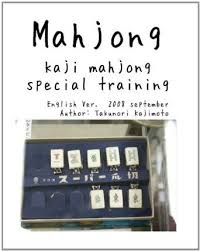
\includegraphics[height=.33\textwidth,clip]{figs/kaji1}

\includegraphics[height=.33\textwidth,clip]{figs/kaji2}
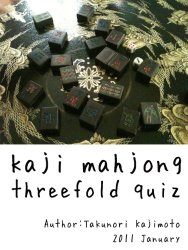
\includegraphics[height=.33\textwidth,clip]{figs/kaji3}

\includegraphics[height=.33\textwidth,clip]{figs/barr2}
\end{center}
\end{figure}



\be \setcounter{enumi}{1}
\i Takunori Kajimoto. 2001. \textit{Mahjong: Kaji Mahjong Special Training.} Kindle Edition.
\i Takunori Kajimoto. 2008. \textit{Mahjong Discard Quiz.} Kindle Edition.
\i Takunori Kajimoto.~2011.~\textit{Mahjong Threefold Quiz.} Kindle Edition.
\i Jenn Barr and Garthe Nelson (ed.~Gemma Sakamoto). 2013.~\textit{A Riichi Mahjong Study Book.} Reach Spirits Inc.
\ee \index{Barr@Barr, Jenn}
Of these four books, I recommend the last one, written and edited by three Western professional players with the Japan Professional Mahjong League. The book contains WWYD problems and discussions as well as quizzes about tile efficiency, waits, and score calculation. 

\bigskip
Their WWYD discussions are a lot more multidimensional compared with stylized hand examples introduced in my book. You would find it interesting to see how Jenn and Garthe often disagree about what they would discard. Even those players who share a similar view on strategy principles can still disagree about exactly how to apply these principles in a given situation. 
You would be able to understand their WWYD discussions much better \emph{after} completing my book first. 

\bigskip
Scott D. Miller, a Riichi player from Texas, has recently published two books on the history, culture, rules, and variants of Riichi Mahjong. I have not had a chance to read them, but both of them seem to be a fun reading. 

\vspace{-2pt}
\begin{figure}[h]\centering
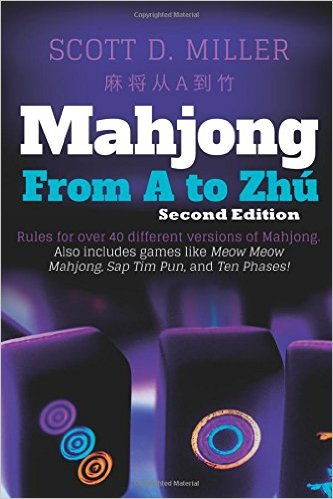
\includegraphics[height=.34\textwidth,clip]{figs/miller1}
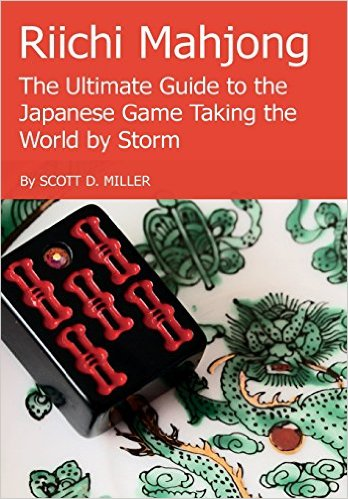
\includegraphics[height=.34\textwidth,clip]{figs/miller2}
\end{figure}
\vspace{-15pt}
\be\itemsep.1em \setcounter{enumi}{5}
\i Scott D. Miller. 2012/2015. \textit{Mahjong From A To Zh\'{u}.} (2nd edition) Lulu.com
\i Scott D. Miller.~2015.~\textit{Riichi Mahjong: The Ultimate Guide to the Japanese Game Taking the World By Storm.} Lulu.com
\ee


\newpage
\section{Online resources}

\subsection*{Osamuko: \url{http://osamuko.com/}} \index{Osamuko}
Osamuko is one of the most extensive online mahjong blogs in English. There are quite a few blog entries there, and many of them are very good. In particular, I find the articles by a contributor named UmaiKeiki very useful. 

\subsection*{Osamuko's Facebook group: \url{https://goo.gl/EMbjwf}}
There is a Facebook group page hosted by one of the contributors of Osamuko. It is a closed group, but I suppose anyone can join the group by sending a request to the administrator. Group members frequently post their play records from {\jap tenhou} and ask for other members' opinions on them. 

\subsection*{Mahjong on Reddit: \url{https://goo.gl/qA5B79}}
Reddit is a social bookmarking website that allows users to add, annotate, edit, and share bookmarks of web documents. It has a lively community dedicated to mahjong where you can discuss mahjong related topics. 

\subsection*{Mahjong News: \url{http://mahjongnews.com/}}
The website is updated regularly with information on upcoming mahjong tournaments (Riichi, MCR, and online), their results, and newly released mahjong books, among other things. 

\subsection*{Japanese Mahjong Wiki: \url{http://arcturus.su/wiki/}}
This website provides an encyclopedic information on rules, terminology, and strategies of Riichi Mahjong. It is a wiki page so anyone can edit the contents. 

\subsection*{Reach Mahjong of New York: \url{http://mahjong-ny.com/}}
This website not only serves as the hub webpage for players in the US but also provides quite a few useful resources, including a terminology list, beginner's guide, and quizzes about tile efficiency and scoring.

\subsection*{Just Another Japanese Mahjong Blog: \\\url{http://goo.gl/3cKpdI}}
This website has a number of articles on Riichi theories, translated from Chinese. 

\subsection*{ReachMahjong.com: \url{http://reachmahjong.com/en/}}
This website is run by the professional players who wrote the aforementioned Riichi Mahjong study book. You can find more WWYD problems and discussions, strategy guides, and reports on tournaments, among other things. 

\subsection*{EMA: \url{http://mahjong-europe.org/}} \index{european@EMA}
This is the official webpage of the European Mahjong Association. You can find information on rules, upcoming tournaments, tournament results and observer reports, and player rankings. 

\subsection*{UKMA: \url{http://ukmahjong.co.uk/}} \index{ukma@UKMA}
This is the official webpage of the UK Mahjong Association. You can find information on the UK Riichi Open tournaments and the affiliated clubs, among other things. 



\end{appendices}

{\small \printindex}

\end{document}

